\documentclass[12pt, a4paper, twoside]{book} % http://ubuntuforums.org/showthread.php?t=1302999
%\documentclass[12pt, a4paper, twoside]{memoir}
%\documentclass[12pt, letterpaper, twoside]{book}
% http://tex.stackexchange.com/questions/16569/latex-document-to-epub-or-mobi-ebook-formats-with-mathematical-formulas
%\documentclass[ebook,oneside,openany]{memoir}

%http://en.wikibooks.org/wiki/LaTeX/Page_Layout
%http://tex.stackexchange.com/questions/86111/pocket-book-size-for-novel-10-8-x-17-5-cm

\usepackage[hidelinks]{hyperref}
\usepackage{graphicx}
\usepackage{multirow}
\usepackage{subfig}

% http://sureshemre.wordpress.com/2010/12/04/latex-book-template-with-fancy-header/
\usepackage{fancyhdr}
\pagestyle{fancy}

% http://nw360.blogspot.co.nz/2006/11/latex-headheight-is-too-small.html
\setlength{\headheight}{14.5pt}

% http://www.karinvandenberg.nl/en/node/22
\setcounter{tocdepth}{0}

%\usepackage[T1]{fontenc}
\usepackage{titlesec}
%\titleformat{\chapter}[hang]{\Huge\bfseries}{\thechapter\hsp\textcolor{gray75}{|}\hsp}{0pt}{\Huge\bfseries}
%\titleformat{\chapter}[hang]{\Huge\bfseries}{\thechapter { | } }{0pt}{\Huge\bfseries}
\titleformat{\chapter}[hang]{\Huge\bfseries}{\thechapter {.} \hspace{1mm}}{0pt}{\Huge\bfseries}

\begin{document}

\frontmatter % page numbers => i, ii, ...
    \title{A Life's Journey Revisted}
    \author{Madge Bray}
    \maketitle

    % Blank page so image is on right page
    \clearpage
    \thispagestyle{empty} % no header bar or page number
    \phantom{a}
    %\vfill
    %\centering[done]
    %\vfill
    \clearpage

    % Front image
    \thispagestyle{empty}
    \begin{figure}
      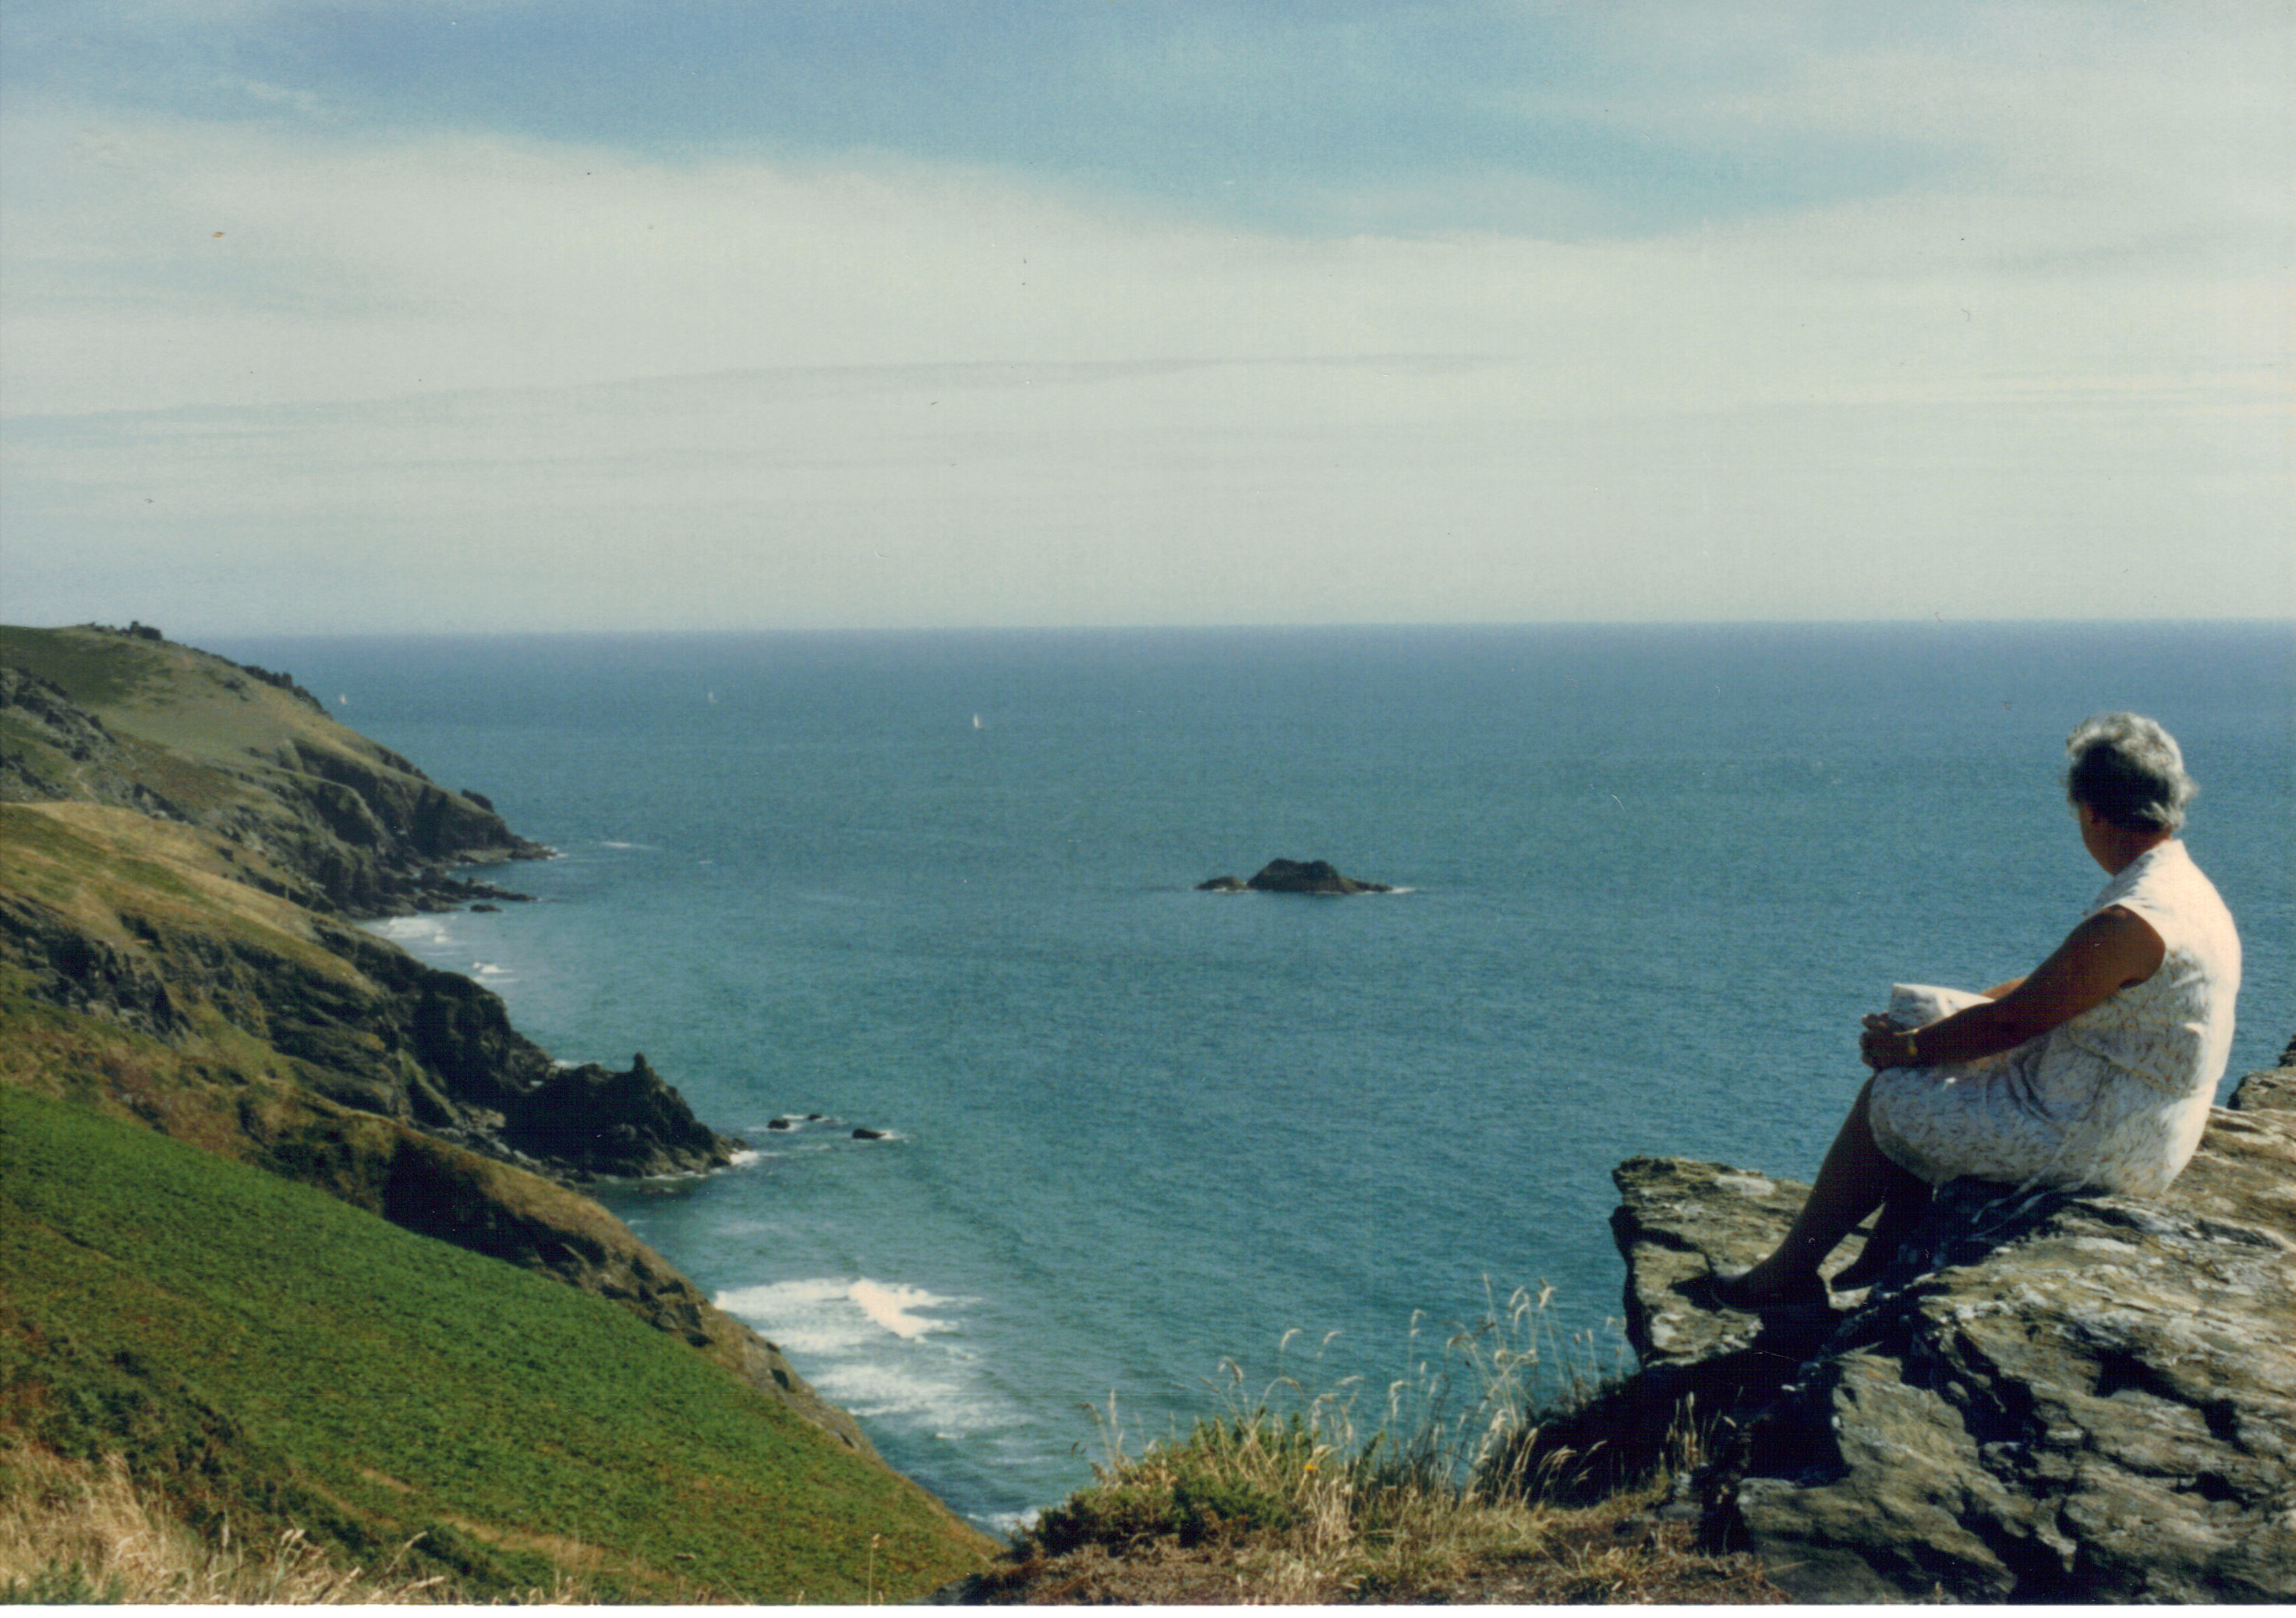
\includegraphics[width=\textwidth]{photos/madge-by-sea.jpg}
      \caption{Madge holidaying in Devon (August 1959).}
      \label{madge-by-sea}
    \end{figure}

    \clearpage
    \thispagestyle{empty}

    \tableofcontents
    \setcounter{page}{1}
    \clearpage
    \thispagestyle{empty}


    \chapter{Timeline}

\begin{description}
    \item[1900] Francis William and Elizabeth May Russell (parents) are born
    \item[1922] Parents are married
    \item[1925] John (brother) is born
    \item[1923] Tony Bray is born
    \item[1928] Madge is born
    \item[1931] Brian (brother) is born
    \item[1935] Geoffrey (brother) is born
    \item[1939] WW2 begins; Madge is 11
    \item[1944] Begins studying domestic science at college
    \item[1946] Begins working as a home service adviser (age 18)
    \item[1952] Meets Tony Bray
    \item[1953] Madge and Tony are married and move to Turkey (age 25)
    \item[1957] Move back to Leamington Spa, England
    \item[1960] Elizabeth Ann (daughter) is born (age 32)
    \item[1962] Arrive in Lagos, Nigeria
    \item[1964] Richard (son) is born (age 36)
    \item[1966] Biafran war begins
    \item[1973] Move to Johannesburg, South Africa
    \item[1984] Trip to Israel
    \item[1987] Move to Durban, South Africa
    \item[1993] Elizabeth \& family emigrate to New Zealand
    \item[2001] Move to Kloof, South Africa
    \item[2008] Eightieth birthday (see appendix~\ref{birthday})
    \item[2009] Tony dies
    \item[2010] Move into Rob Roy Retirement Village
\end{description}

    \chapter{Foreword}

A couple of years ago, when I asked mum to consider writing her
memoirs, she protested vociferously that her life wasn't interesting
and no-one would want to read about it. I told her that in fact she
owed it to her grandchildren as a legacy and that I was sure they
would be interested. And so, after some more persuasion, she rose to
the challenge with her characteristic gritty resolve and started
writing.

I have only recently realised that mum is one of the most courageous
and resilient women I have ever known. Like many of her generation,
she has often had to cope with very challenging
circumstances. However, she not only continues to deal with what life
throws at her, but invariably finds a reason to be grateful and happy
with her lot. Many of us could take a leaf out of book!

Mum has a very active mind. She took great delight in sharing dad's
love of astronomy, enjoys a robust discussion about current affairs
and, in particular, follows the international tennis circuit with
great enthusiasm. She is also very creative and her outlets have
included playing the piano, sewing and cake decorating. Clearly she
also writes a good story!  However, her writing has also extended to
creating poems for various occasions, one most notably being her 80th
birthday celebration.

In writing her memoirs, mum has provided an insight to a varied and
interesting life and has revealed the character and determination that
I so admire. Often families know very little of the life behind the
older generation and I am so pleased that mum took the time and effort
to put pen to paper so that questions about her life can be asked and
answered while it is still possible. I am very privileged to have her
as a mum (although I admit I haven't always thought so!).

I have been amazed at the level of interest mum's memoirs have
generated. Mum's initial writing prompted questions which required her
to write some more until she finally cried ``stop!''. I could not have
foreseen how the project would gather momentum and become a true
collaborative effort among her grandchildren. So thank you mum for
rising to the challenge and to all the kids for the part they have
played in bringing this all together -- the typing and editing,
finding and scanning photographs, and research even, which uncovered a
newspaper article about the bombing in Lagos! A mammoth task, but the
result is a beautiful book, a tribute to mum's life captured on paper.

Liz Preston

July 2013



\mainmatter  % page numbers => 1, 2, ...
    \chapter{Childhood}

My parents, Francis William and Elizabeth May Russell, were both born
in 1900 and died aged 83 and 90 respectively.

My dad's father owned a shoe shop selling and doing repairs in a small
village called Broughton in Hampshire. He was also a lay-preacher
which was more important to him than his shoes!

I never knew my mother's father for he died when he was 41; a rose
thorn caused him to have blood-poisoning. The poison passed up his arm
and caused a terrible infection. There were no antibiotics in those
days. My mum missed him terribly as she adored him (and he
her). Shortly before he was ill, he told my mum what had happened to
the Titanic. She was twelve years old.

My mum came from farming stock and her brother and mother (a widow)
ran a farm near Romsey in Hampshire and it was there that I spent a
lot of my school summer holidays working on the farm and taking tea
and sandwiches to the men. There was no automatic machinery then so
the farmers had to rely on the marvellous shire horses and manual
labour (including me) to work in the fields. The war took a lot of men
away. My mum left the farm to be a secretary at an office in Swanage,
Dorset and it was there that she met my dad who worked in a rates
office. A paper had to be delivered to his office and she asked to
take it across. Her boss said ``Ah yes, I think you've got your eye on
that nice young man over there!'' They were married in 1922 and my
brother John was born in 1925 followed by me in 1928, my brother Brian
in 1931, and Geoffrey in 1935.

I have no way of remembering anything before I was about five years
and I suppose this is normal. I have a lovely memory of learning to
ride a two-wheeler bike, after getting around on a three-wheeler which
the four of us used. I sat on the bike one day and my brother, John,
guided me round the garden and I suddenly realised I was on my own,
what a thrill! I learned how to tie my shoelaces on the same day. From
that day I lived on a bike -- the whole family rode and even my mother
used to go shopping with a big basket on the front of hers. There was
never enough money for new bikes so when one was needed my dad went to
the market and bought two old ones (for 10~shillings) and would
cleverly put parts together to make one new one, I didn’t realise just
how clever he was; he had a way with repairing sewing machines,
clocks, getting new soles on shoes and he was also a self-taught
organist playing every Sunday in a village church for 42~years. How I
wish I could have given him a pat on the back sometimes -- but I don't
think children are like that.


\chapter{The War}

I was 11 when the Second World War began and I shall never forget the
horror of hearing the bombs coming down. We lived in Hampshire in the
south of England and were surrounded by targets attractive to the
enemy. 47~miles from London we could see the glow of it burning and
the night times were the worst. We had to have special covers made for
the windows for there was not to be a single chink of light. Wardens
had to be on patrol during ``air raid warning red''. What a relief
when the ``all clear'' sounded – a hideous – sounding siren.

We were on rationing, of course, and had to be issued with coupons -
not only for food but for clothes, furniture etc. Rations were poor
but it is said now that if we all ate like that now, we would all be
much healthier. The weekly rations were 2~oz. of sugar,
4~oz. margarine, 2~oz. butter, very little meat, and 1 egg! Having
collected rations for us all my mother would mix the butter and
margarine together (she bought a special pair of butter ``pats''). I
would love this job too! I remember her as being a most practical and
resourceful woman with never a complaint about situations. It must
have been such a worry to bring up 4~kids at this time with the threat
of bombs etc.  but her brother -- my uncle -- a farmer near
Southampton, would send us a chicken or a rabbit skinned and cleaned
for the oven. In those days there were 2~postal deliveries in the day
and what a thrill it was to know there was food coming when that red
postal van stopped outside the house! Nowadays a chicken is everyday
food but then it was a luxury and turned into a nourishing meal for 6!
Good for my mum -- I wish I could have appreciated her more. Why does
one have to have regrets?

Of course, I was too young to join up -- I would have loved to have
been in the WRENS\footnote{Womens Royal Naval Service} but I had a
different kind of war work which was fun. People had to learn how to
deal with broken limbs (as a result of bombings). So I volunteered to
attend twice weekly sessions of being rescued, splintered etc. The
worst part was being showered and carried along draughty corridors on
a stretcher. This operation was to wash off the poisonous gas expected
from the skies; I was never so clean in my life! (The gas never came)
we had to carry gas masks at all times and, when we practiced, we all
looked like pigs!

On Saturday mornings, we children had to go and queue up for saccharin
tablets\footnote{A sugar substitute.} and with long queues, this took
a long time.

On ``Battle of Britain'' day we went to my uncle's farm for the day
and it was only later that we realised it was an historic day. There
was to be an onslaught from the Germans but our wonderful Spitfire
pilots shot down very many of the bombers. In Winston Churchill's
words ``Never has so much been owed by so many to so few''. What a
wonderful man Mr Churchill was. I shall always remember his
encouraging words and messages.

In the midst of all this war nonsense, life had to carry on with
school, work etc. Just at the time when war was declared (Sept 1939),
I started going to Farnham Girls Grammar School. This was to involve a
daily journey (10~miles) starting with a bike ride to the train
station ($1\frac{1}{2}$~miles) and the train ride to Farnham. My bike
went into Mrs Newbold’s shed until I collected it in the
afternoon. She was a wonderful person -- a great friend of my mothers
-- how many times did she hold up the teapot as I went to collect my
bike? There was never any question of a car lift to school or to the
station. I think my dad had a car then but there was severe petrol
rationing. I am pleased to say that even on the icy roads of winter I
never came off my bike! I was not a remarkable pupil at school and was
taken off the clever subjects like latin, math, etc. and put into
domestic science which was not a bad thing because it set me on the
road to my career.

Why I should remember a little man -- the Reverend Tonks -- I have no
idea but memories are made up of people and events. I was fifteen at
the time and my parents agreed that I would play the organ (just a
little Harmonium) at Sunday morning services. I got 10 shillings for
each service -- I was rich indeed! It was winter and I had to cycle
six miles through ice and snow to get to a village called Newton
Valence. Just outside my home town of Alton, Hampshire. But Mr. Tonks
was a character (almost Dickensian) and I remember that he wore white
socks under his priestly robes!

At the services, there were only three people -- himself, the church
warden, and me and, since it was decreed, we had to worship; I am not
sure if he preached a sermon. He was such a jolly little man and I am
sure the Lord was pleased with him; he deserved a larger congregation
but who could blame anyone for not turning out in that awful weather.


\chapter{Adulthood -- Gloucester}

To pursue my best interests, it was decided that I should ``do''
domestic science (today it is called home economics) and this involved
studying all aspects of home management (two years) and then followed
a short course in cookery demonstrating which I passed without
difficulty. In fact I loved it and found it interesting that the more
nervous I felt before a demonstration the better the result (I
understand this theory applies to other aspects of performance, for
example acting). I did not enjoy my demonstration exam. The subject
was the use of soya (of all things!). The main reason was that those
in front of me were fellow students who were prepared to giggle and
take the mickey. However, all went well and I passed out (not
literally). The whole time I was at the domestic science college in
Bath was wonderful and I made good friends, some of whom of course
have passed away. But how perceptive it was of my parents not to
persuade me to pursue anything academic -- a lost cause anyway!

After training college in Bath, I took up a position as home service
adviser, first of all in Luton and then in Gloucester for 6 years. It
was a wonderful life and I was full of bounce and confidence (see
Picture~\ref{madge-adult})!

\begin{figure}
  \centering
  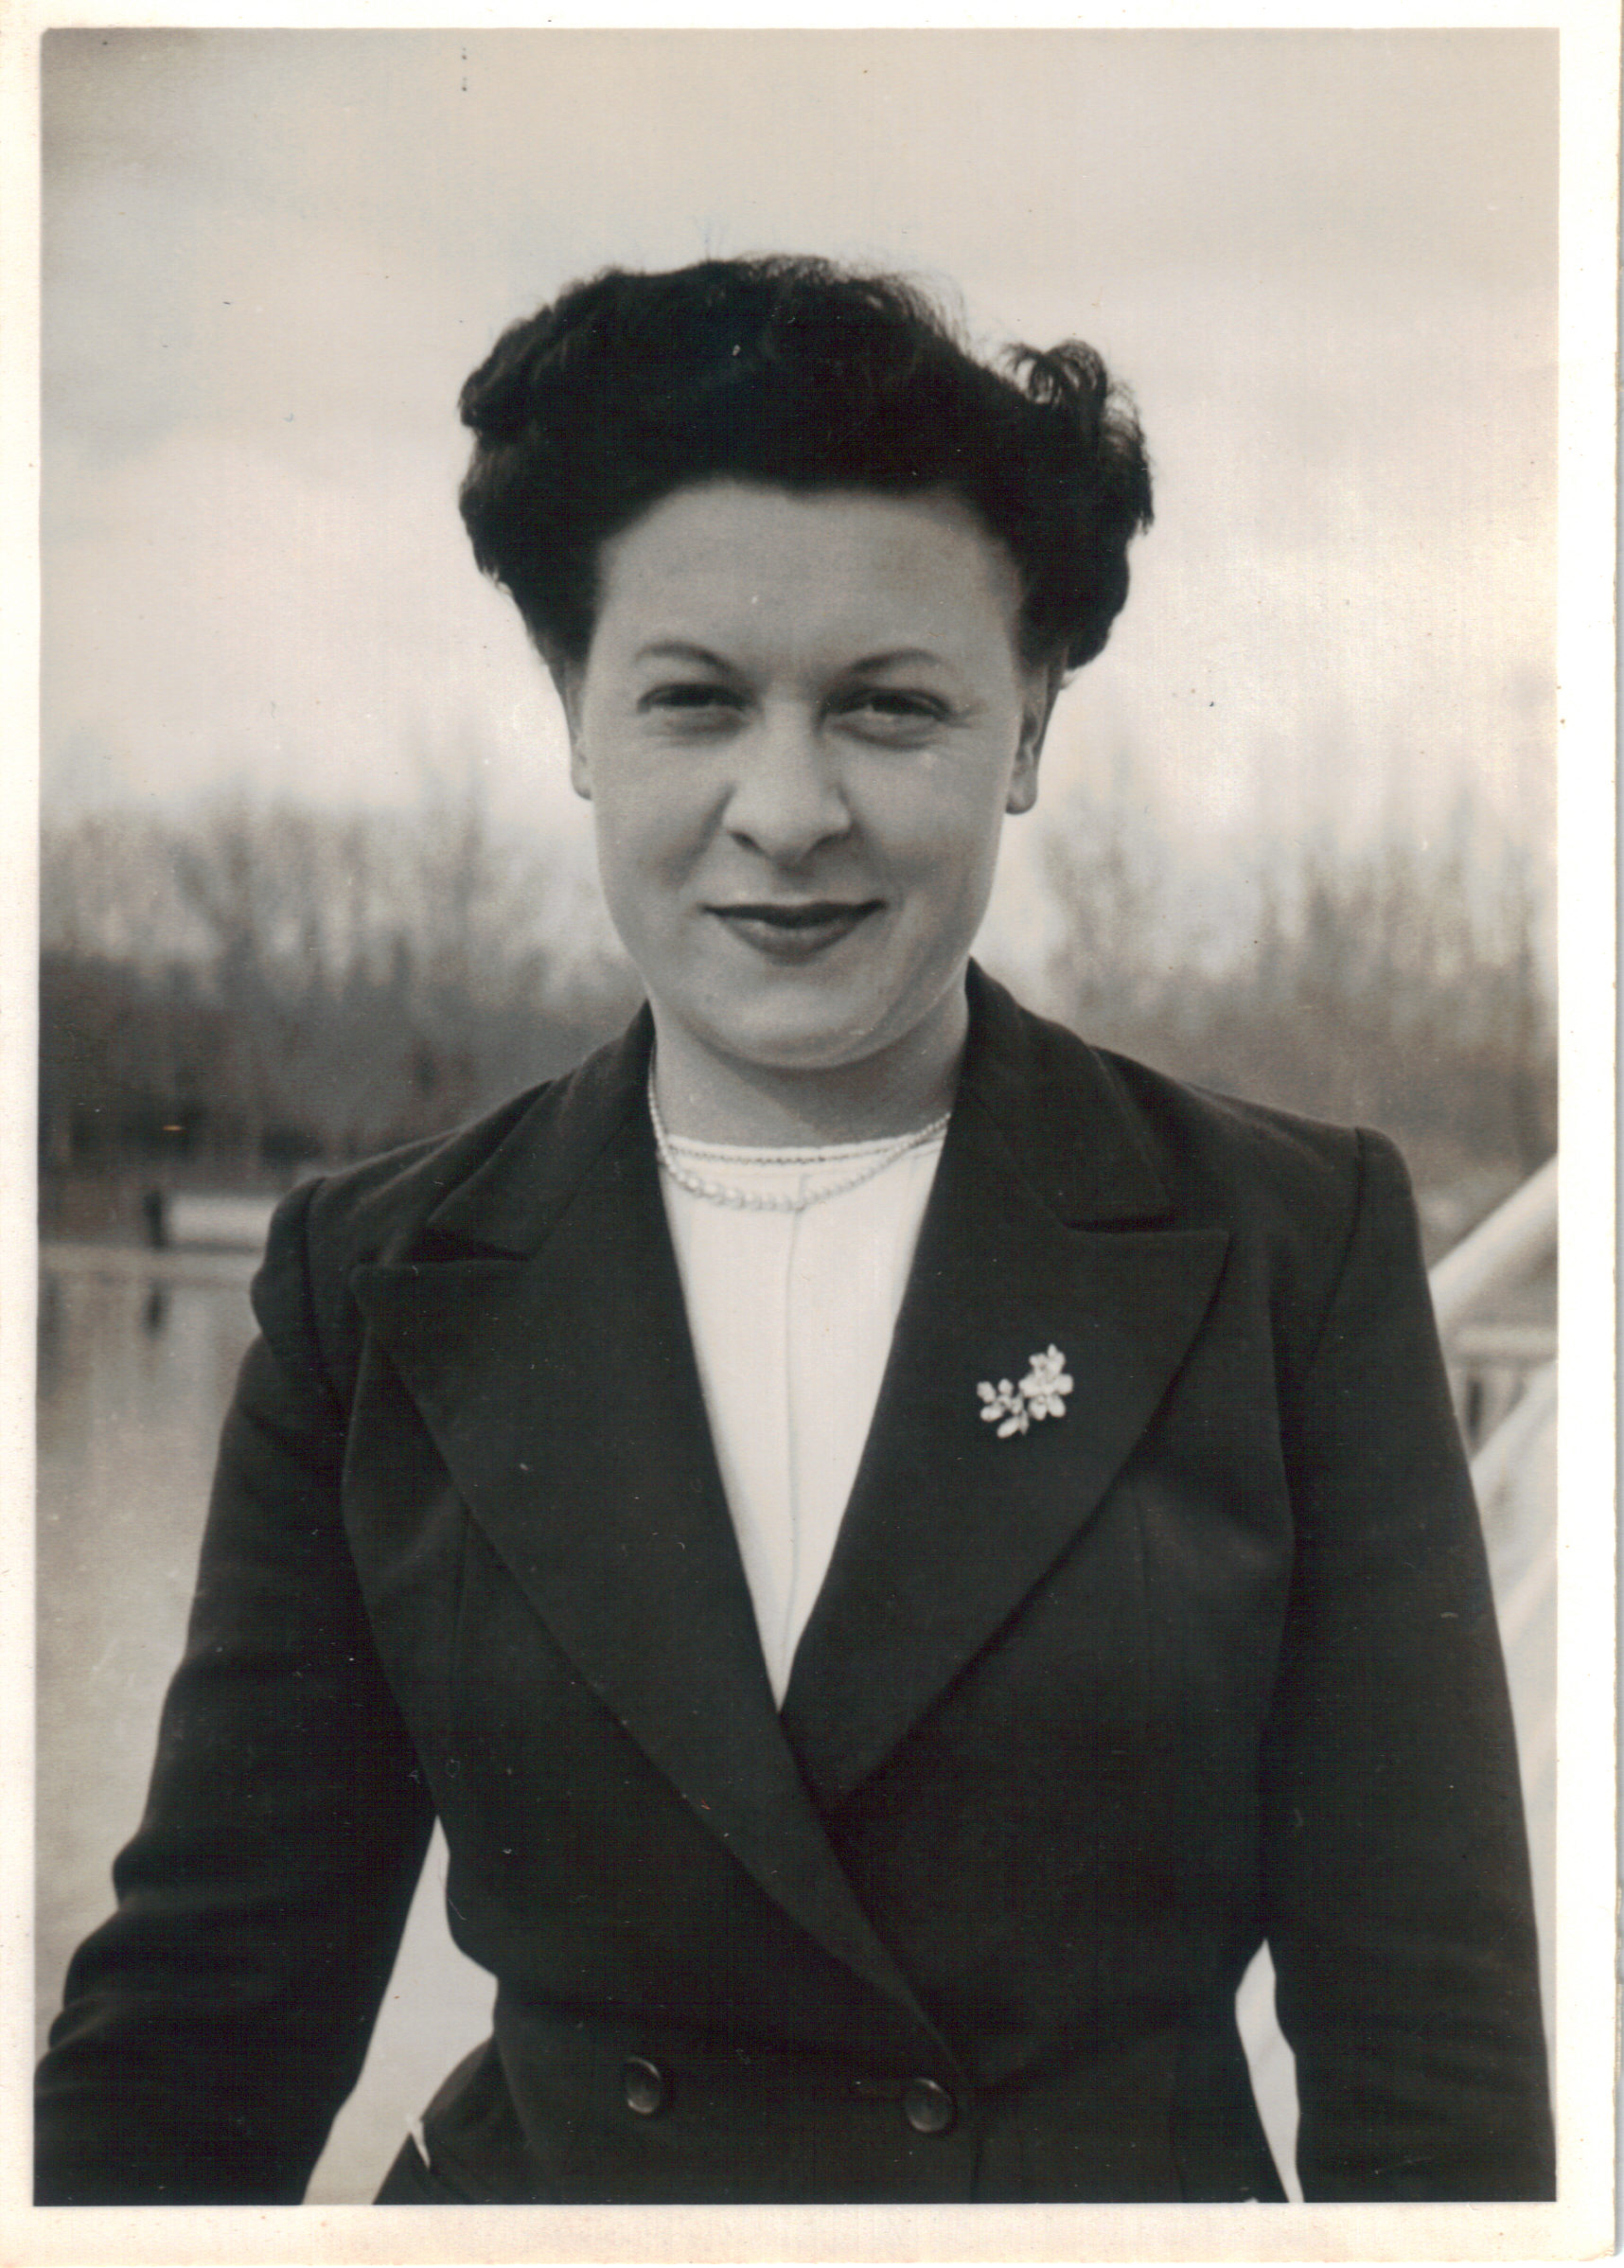
\includegraphics[width=0.95\textwidth]{photos/madge-adult.jpg}
  \caption{My first glimpse of Turkey (1953).}
  \label{madge-adult}
\end{figure}

I was with the gas company and we had a beautiful demonstration
kitchen where we held regular ``dems''. Going out into the country to
talk to women's organisations was more difficult as I had to catch a
bus loaded with my equipment. It was however, lots of fun especially
when things went wrong (for example, failure to add some ingredients,
like baking powder).

These days one would be provided with a car! But it was useful to have
to sign off on a country expedition in order to catch the bus back to
Gloucester because if anything went wrong with the demonstration I was
able to say ``you see what will happen to you if you do not take care
of preparation -- in any case I have a bus to catch now''. What a
career! Demonstrations on TV these days are so much more sophisticated
-- but I am appalled that the clever and deft top class demonstrators
do not tie back their hair -- there is too much hair falling about and
it was always the rule that it should be kept out of the way of
food. But oh! What lovely delicacies they produce.

Because of the war (which was then over) there was not much food to
demonstrate with and I had to resort to things like parsnip pastry
(!), potato scones (!), fat-less sponges, etc. I marvelled at the
confidence I had; with age it dwindles away.

I have always been interested in acting and the theatre and was in
several plays at school. I was good at ``learning by heart'' and could
learn the other actors' words as well as my own. The thrill of the
curtain going up was always tremendous and I believe that the nervous
sensations felt at this moment can be felt by top performers as well
as by amateurs and, in fact, I can relate to this by my feelings when
I was due to begin a cookery demonstration many years later in
Gloucester; if I did not feel sick with nerves and wish I were a
million miles away the demonstration would not go well. In these
circumstances, one has to win the audience over in the first minute
and ``make \'em laugh'' -- then all should go well.

Whilst in Gloucester, I joined an amateur operatic and dramatic
society -- known as ``The Gods''.

The society put on many delightful shows and I loved taking part in
the dramatic side of things -- although I did have a ``walk-on'' part
in ``The Quaker Girl.'' In one comedy (heaven knows which one) I had
to appear briefly in my underwear and shout ``Flags for the
lifeboats.'' It was hilarious! There would sometimes be a bouquet for
me at the closing curtain of a show. No matter that it might be from
someone anonymous -- the thrill and the glamour were there.

The gas company where I was working in Gloucester started a concert
party and I was invited to join as the resident pianist (we called
ourselves ``The Thermites.'' I ask you!).

My gift of being able to play the piano ``by ear'' came in very
useful. We had so much fun doing sketches etc. We would go out into
the country and our audiences showed their appreciation for good,
clean fun and would often provide us with lovely refreshments after
the show! In one particular cold and draughty church hall, the piano
was tied up with pieces of string but it still gave out a good sound!
There was nothing professional about us but we had such a good
time. In the middle of all this I left to get married -- I don't know
if they found another pianist!

I was lucky to become friendly with Alma and John Hoare. John worked
in the gas company's office. I spent every weekend with them; weekends
are the hardest when living alone. I shall always remember their
kindness and hospitality. One Sunday morning, Alma told me they were
to have a visitor -- a young man on leave from Turkey.


\chapter{Love}

\begin{verse}
``In 1952 one day, into my life came Mr Bray''
\end{verse}

If ever anyone tries to argue that there is no such thing as love at
first sight refer them to me!

I was demurely sewing in the lounge when I heard his voice and then
seeing Tony, my pulse raced. In that moment I knew that this was the
man with whom I wanted to spend the rest of my life. He was so
handsome and charming but best of all, I noticed his highly polished
tan colour boots, Oh golly! I think I almost fell in love with his
boots! We exchanged the minimum of greetings but I had seen enough.

He asked me out seven times before he had to return to Turkey but
during that time, we had agreed to marry... On a moonlit drive (in his
hired car) I did a very daring thing and told him I had something to
confess. He must have had a host of thoughts. I told him that I had
fallen in love with him! Everything came together for us and I
couldn't bear the thought of him going away but he had to return to
Turkey and his telecommunications job.

\begin{figure}
  \centering
  \includegraphics[width=\textwidth]{photos/madge-wedding.jpg}
  \caption{Tony and Madge on their wedding day (June 20, 1953).}
  \label{madge-wedding}
\end{figure}

Tony was not close to his parents and I think that was because his
mother kept herself apart. Tony called her ``Fan'' and his father
``Reg''. Reg was a perfect darling and was very fond of me. Tony was
one of a twin but his sister, Pamela, died when she was nine days
old. I thought that when Tony met me Fan would have a good opportunity
to look upon me as her lost daughter but she did not take to me -- in
fact, she disliked me and resented my taking Tony away from her. I did
everything I could to help her, especially when she fell off a bus and
broke her leg -- she had to wear a caliper which was a terrible
impediment. Reg was very kind to me and reckoned I was a ``good
catch''. He died when he was 69 and I lost a good friend and ally.

I took the children to stay with Fan when we were on leave from
Nigeria and worked really hard. She never 100\% took to Elizabeth and
did not recognize Richard! It must be awful to harbour such feelings
against someone as she did to me. I have forgiven her but it would
have made life so much more pleasant had we been on friendly terms. We
did not go back to England when she died. Instead we went and sat in
the church in Lagos at the time of the funeral. I noticed that Tony
did not cry as he did when his father died. I hope Fan is happy in her
afterlife and I wonder if I shall meet her.

There were promises to write but he fell short of this because of the
demands of his job. However glorious arrangements of flowers would
arrive and helped me to forgive him. We had met in January and in
December he asked me to fly to Turkey (and paid my fare -- 100~pounds
-- a lot of money in those days) so I had the opportunity to see the
country where I was to live for three years after our wedding in June
1953. It was my first experience of being overseas and so different
from life in England. The train journey from Istanbul to Ankara (13
hours on the wagon lits) was so romantic and different. I was
transported to another world. Leaving him after the two weeks holiday
(I stayed in the flat where Tony lived with a colleague and his wife)
was unbearably sad. But, after a while I began to enjoy the flight
home. I was the only passenger on the leg from Istanbul to Athens and
was invited to go up front with the crew. I remember laddering a
stocking then! On the poor old Viking aircraft (which was actually a
very reliable plane) we had to have a nights stop in Rome and I was
taken round to see the sights by this very friendly crew.

Life had to return to normal after arriving in England but what a
wonderful memory Turkey was. And what a lot I had to look forward to.

Six months of waiting and planning followed and preparations were made
for our wedding. I went to London to meet Tony on his return from
Turkey and we had a few lovely days on one of which we went to Charles
Packer in Regent street to choose the engagement ring -- a lovely
three stone diamond ring. I was so excited!

Our wedding was a great occasion and held in the assembly rooms in
Alton (see Picture~\ref{madge-wedding}). I could not help thinking of
those other dark days of the war when, in the lower regions of this
building I had been carried on a stretcher to be splinted and bandaged
and showered and carried along the draughty corridors.

We were due to have a honeymoon in Cyprus but there was trouble there
and, after a few days in Haslemere, we flew direct to Turkey. The old
house we stayed in at Haslemere (the house was called ``Undershaw'')
had been owned by Sir Arthur Conan Doyle who was the creator of
Sherlock Holmes and his murder mysteries. Occupied now by old ladies
living out their quiet days of retirement. They took no notice of us
-- or, if they did, they may have guessed that we were on honeymoon
and might have recalled those blissful days of their own. I well
remember the spirit lamps on their breakfast tables to keep the tea
hot!

% \begin{figure}
%   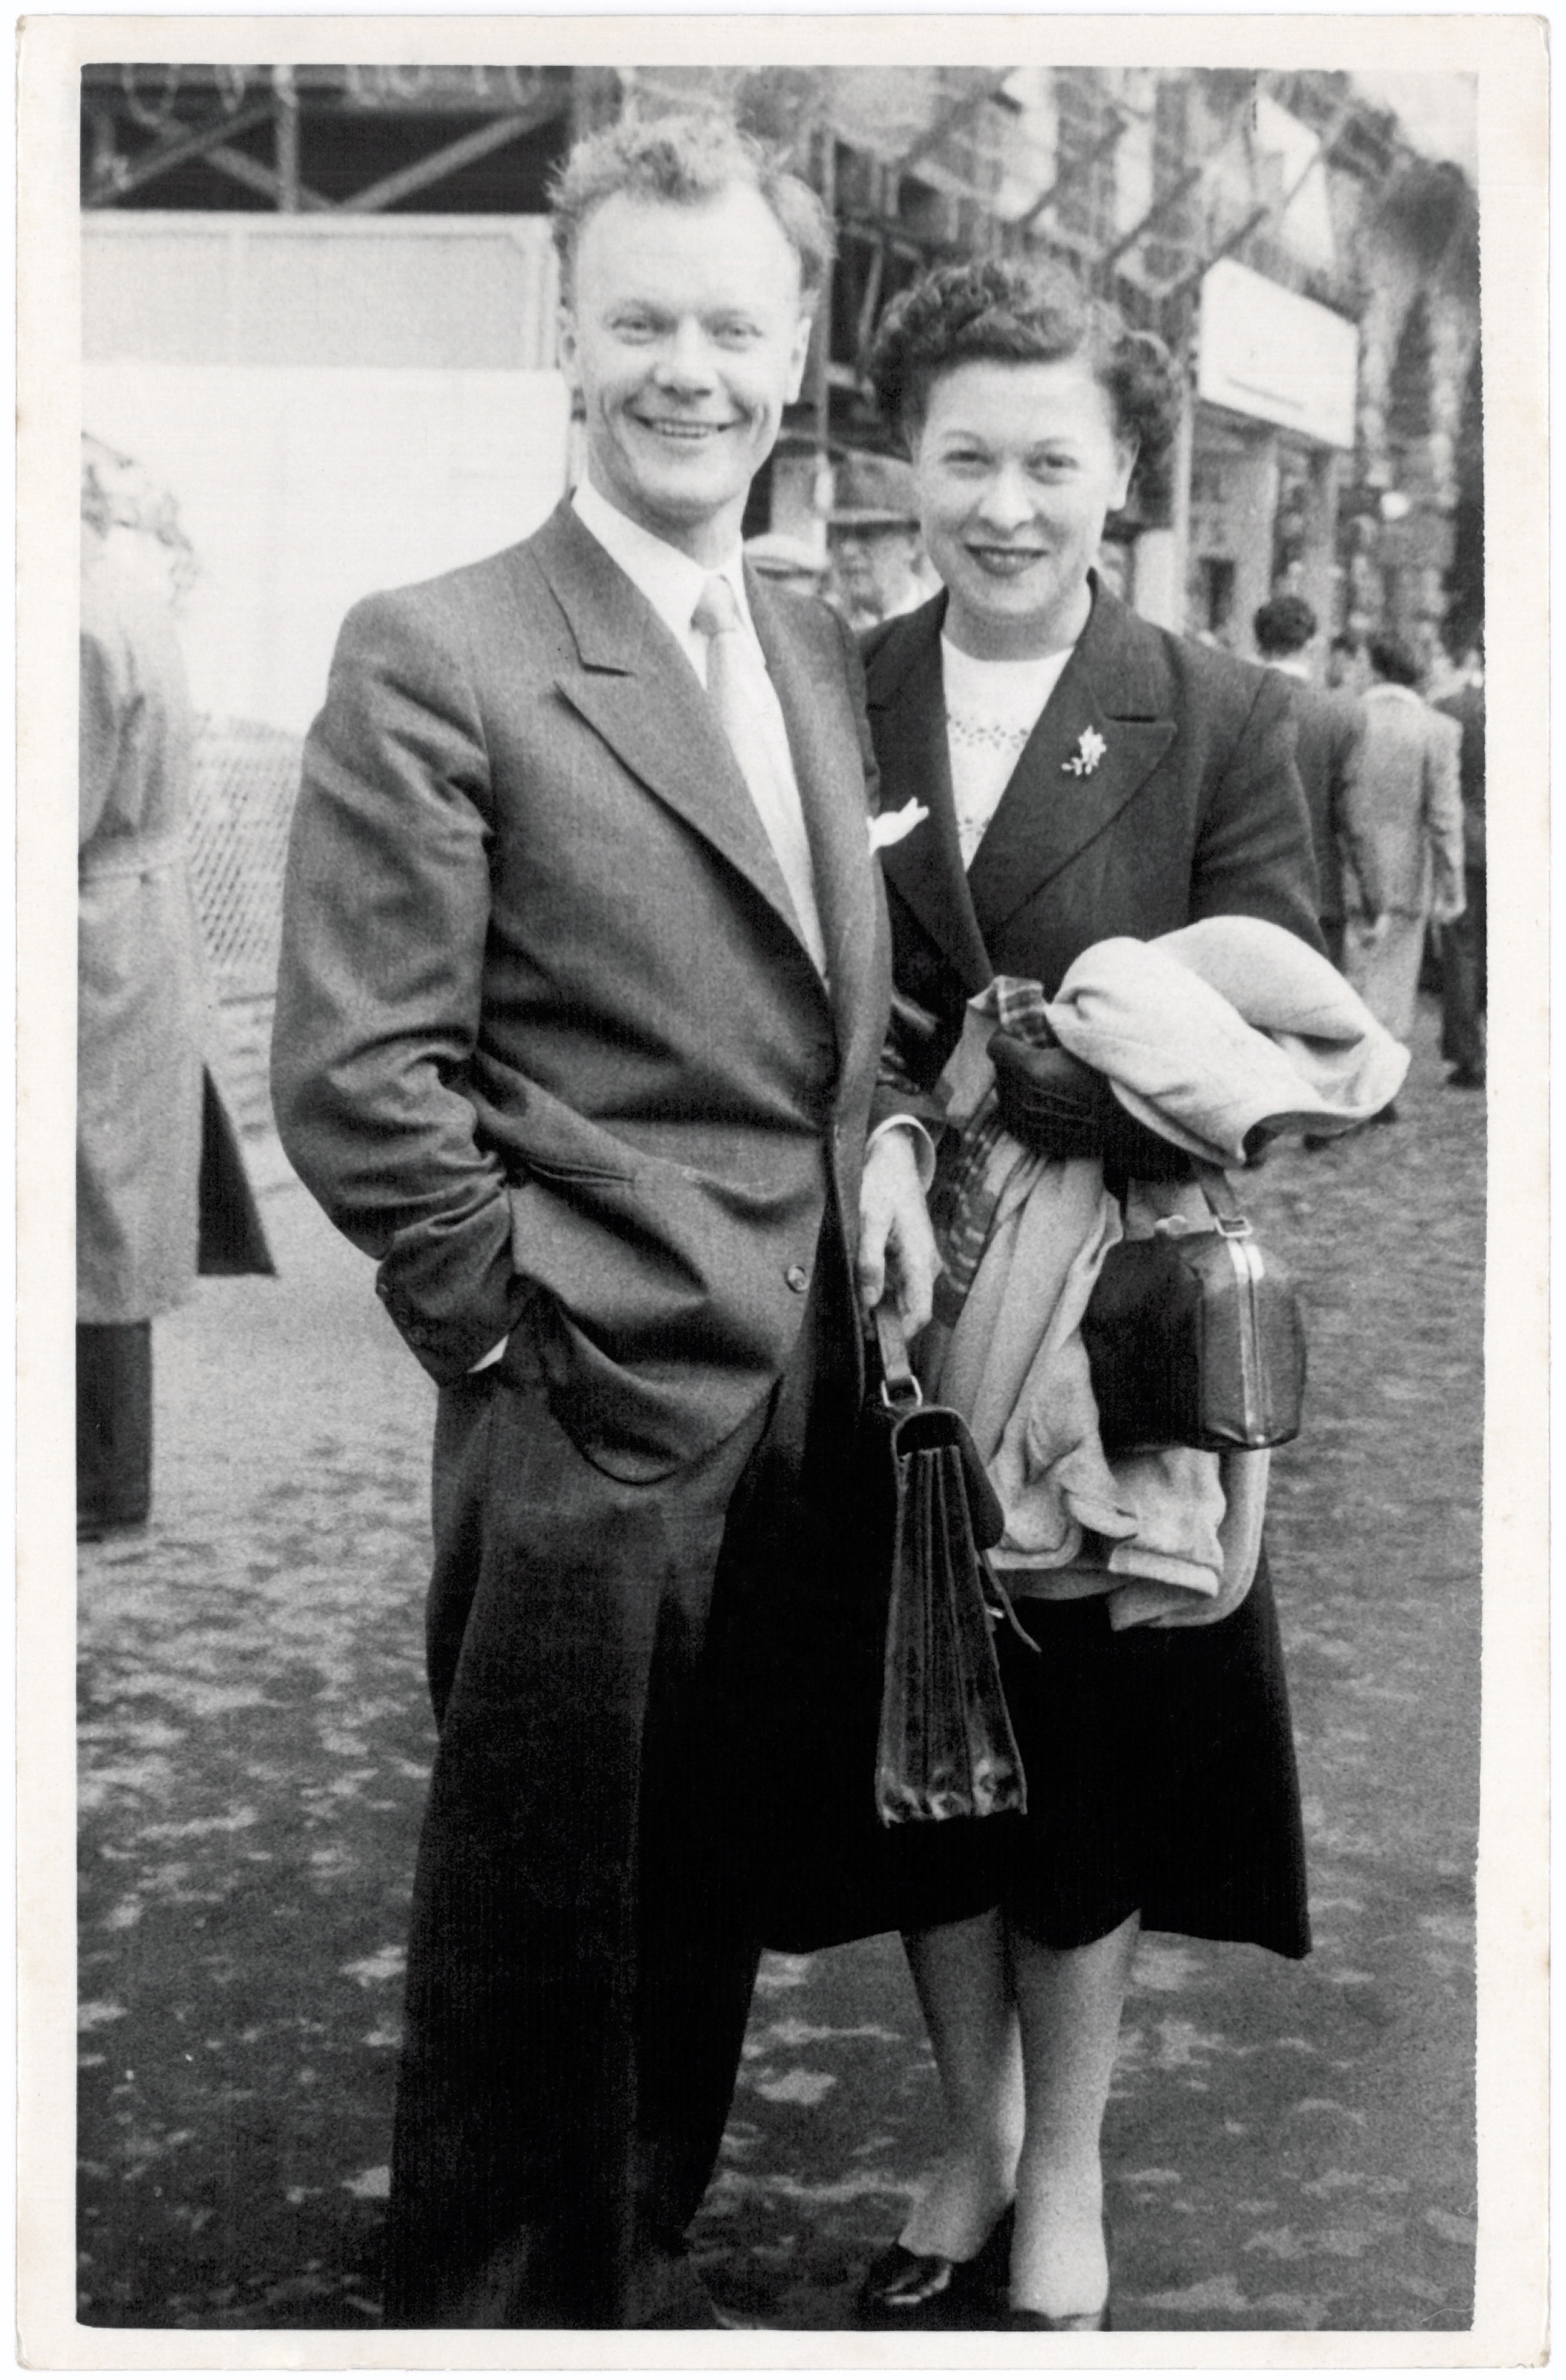
\includegraphics[width=\textwidth]{photos/tony-and-madge3}
%   \caption{Tony and Madge 3.}
%   \label{tony-and-madge3}
% \end{figure}

% \begin{figure}
%   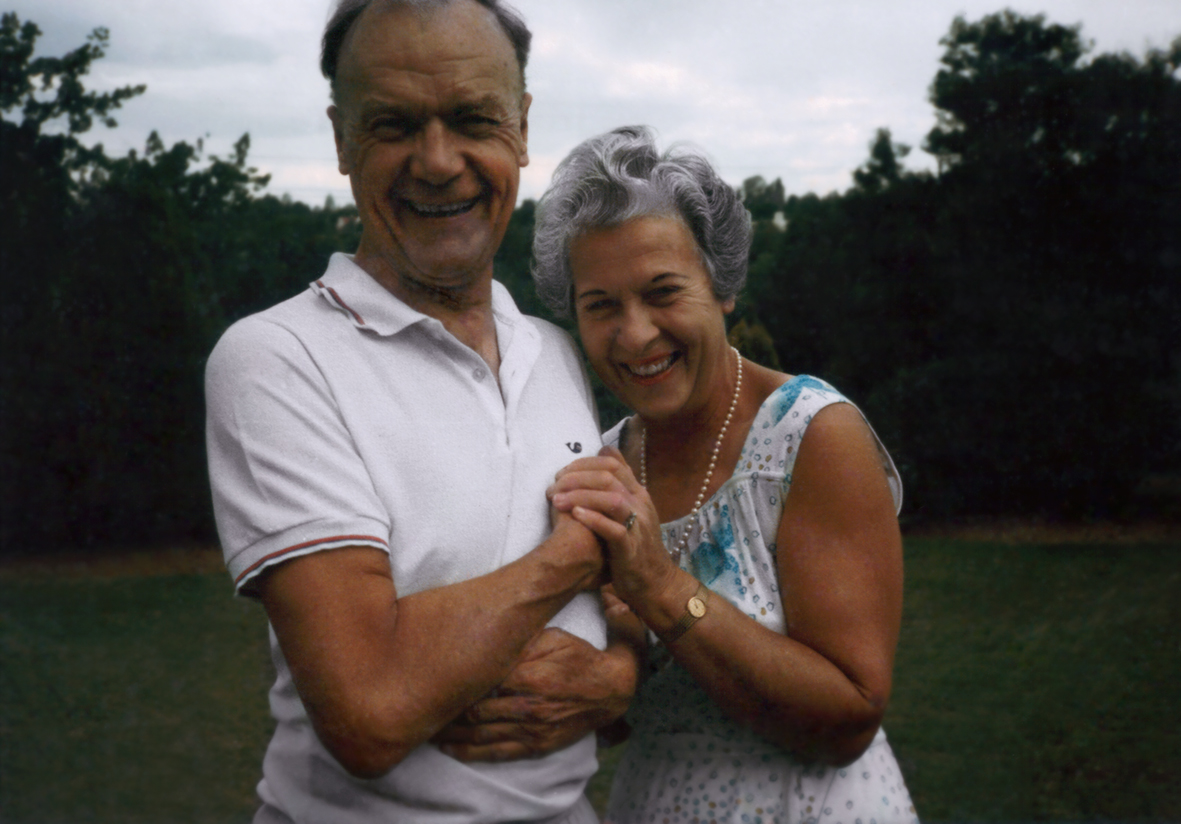
\includegraphics[width=\textwidth]{photos/tony-and-madge2}
%   \caption{Tony and Madge together (19xx).}
%   \label{tony-and-madge2}
% \end{figure}

% \begin{figure}
%   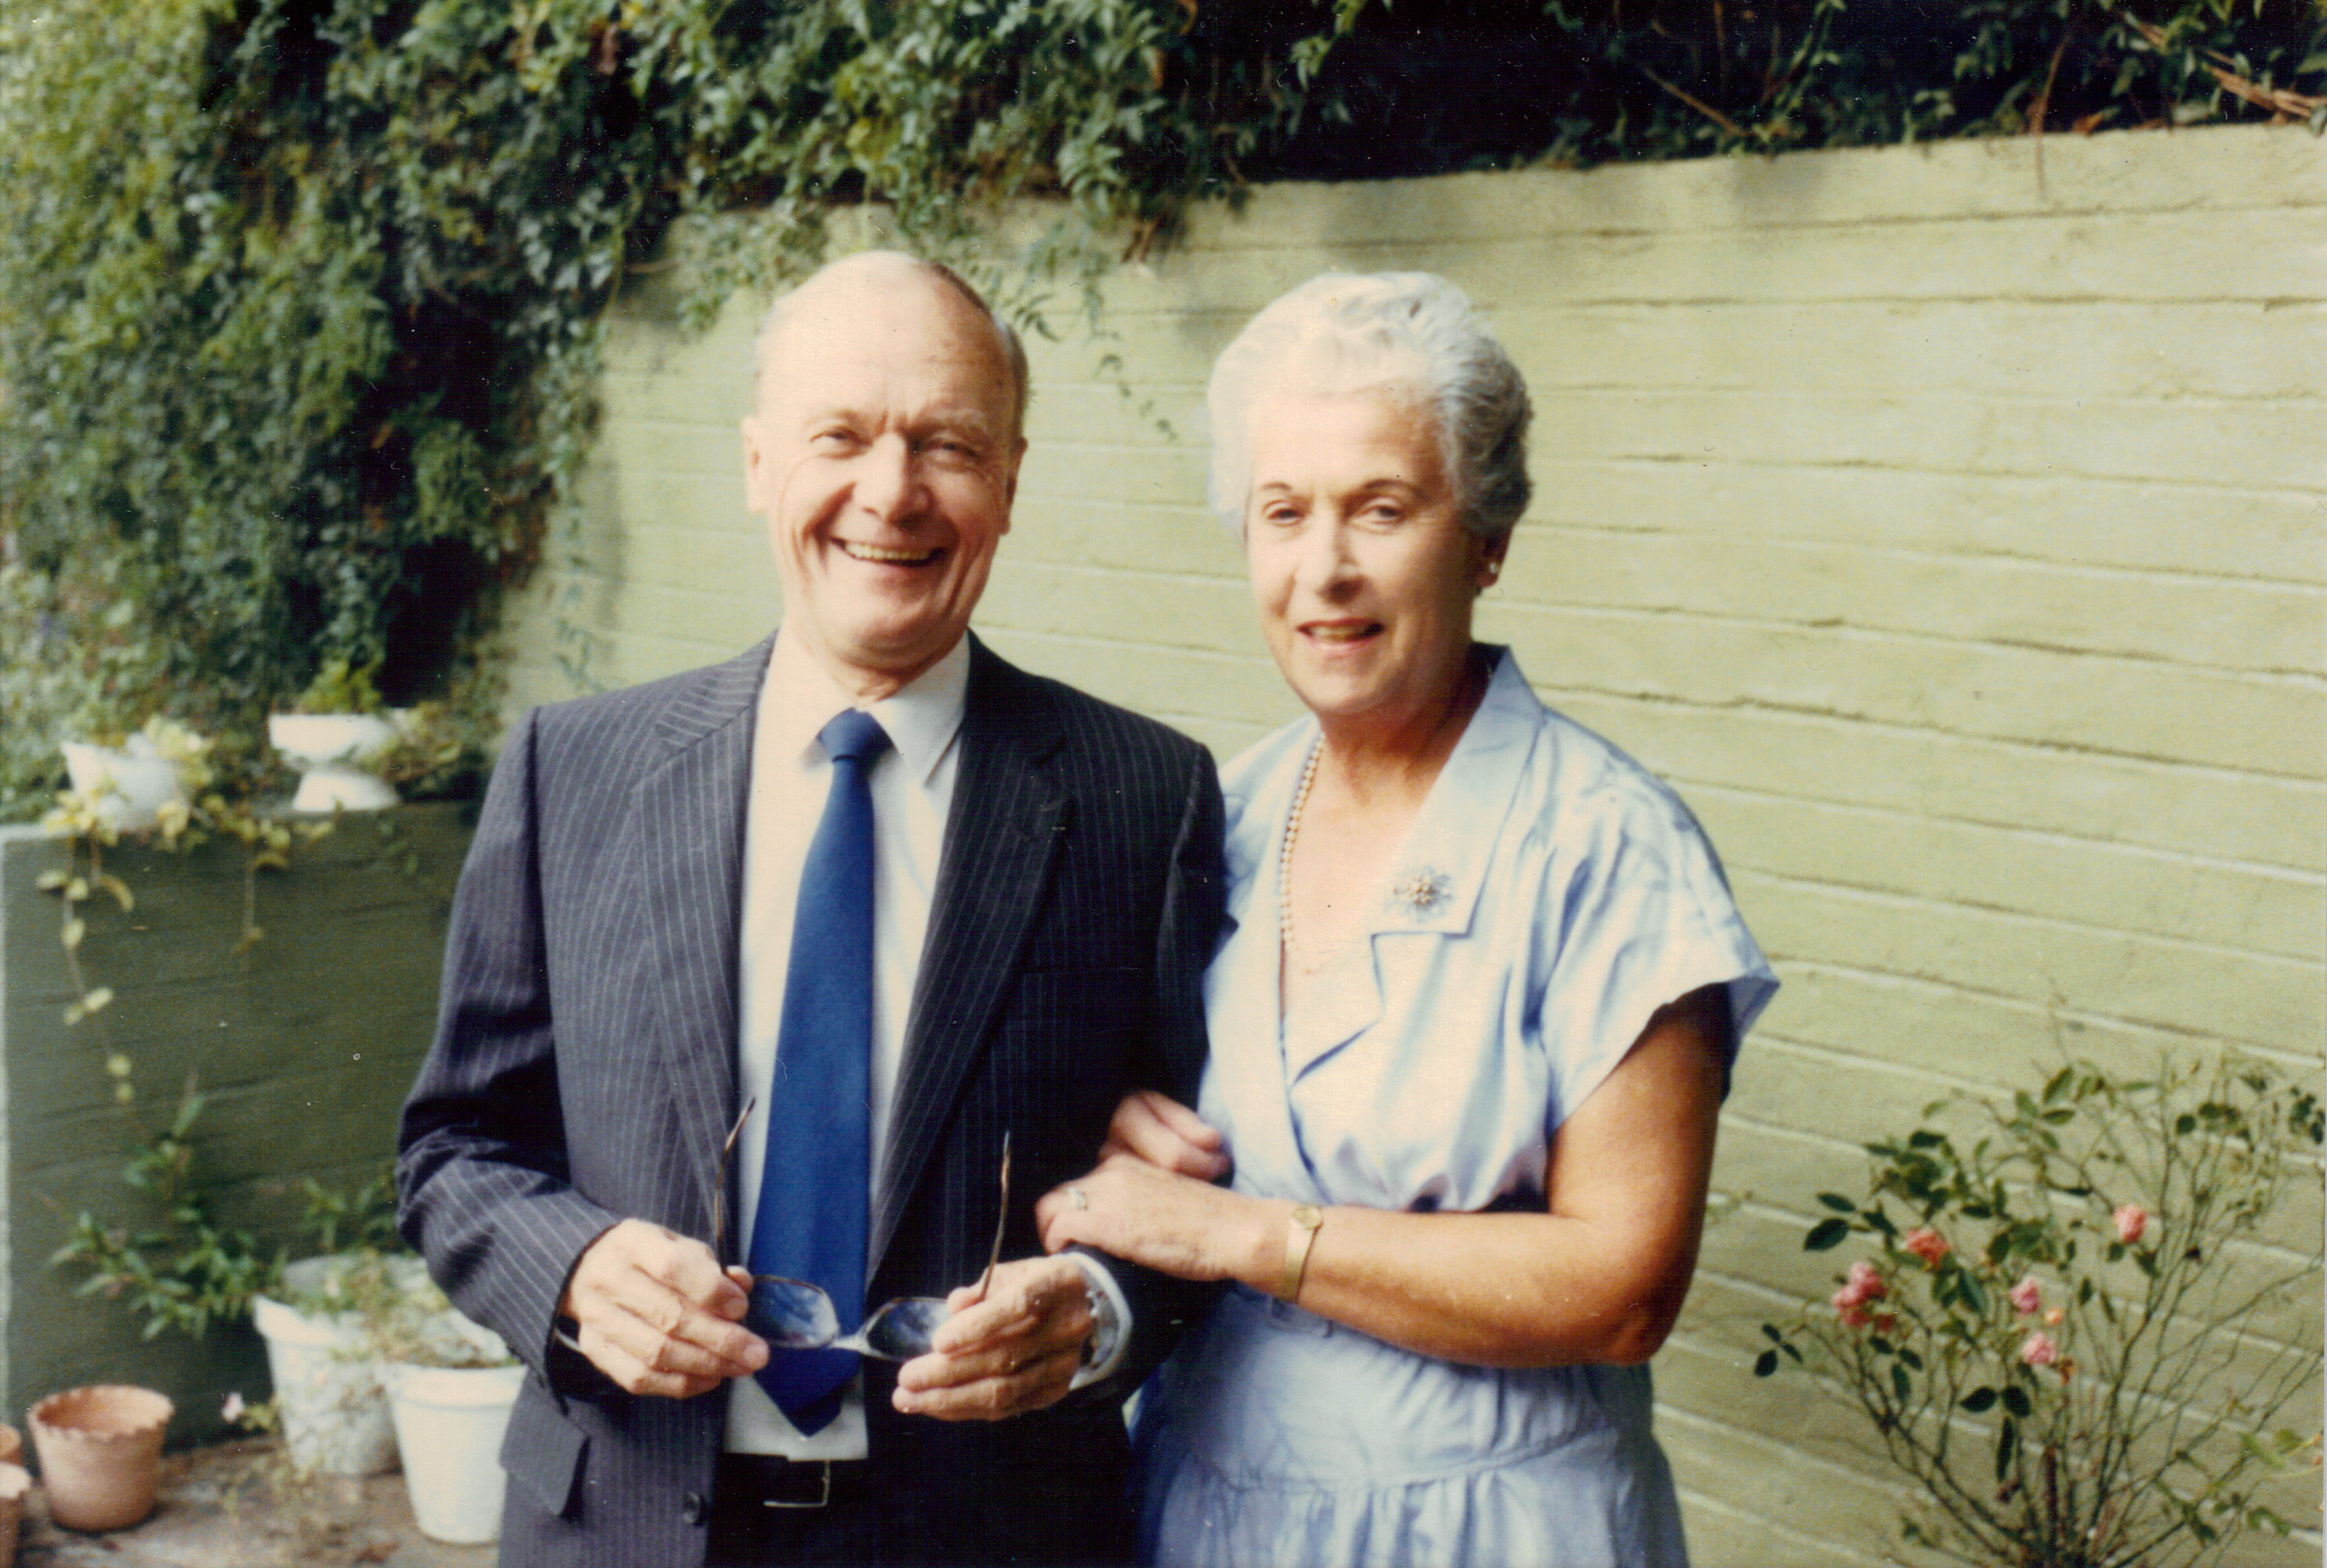
\includegraphics[width=\textwidth]{photos/tony-and-madge}
%   \caption{Tony and Madge together (19xx).}
%   \label{tony-and-madge}
% \end{figure}
\begin{figure}
  \centering
  \begin{tabular}{cc}
    %\multirow{-2}[41]{*}{   % For a4 paper
    \multirow{-2}[32]{*}{    % For letter paper
      \subfloat[In London buying the ring.]{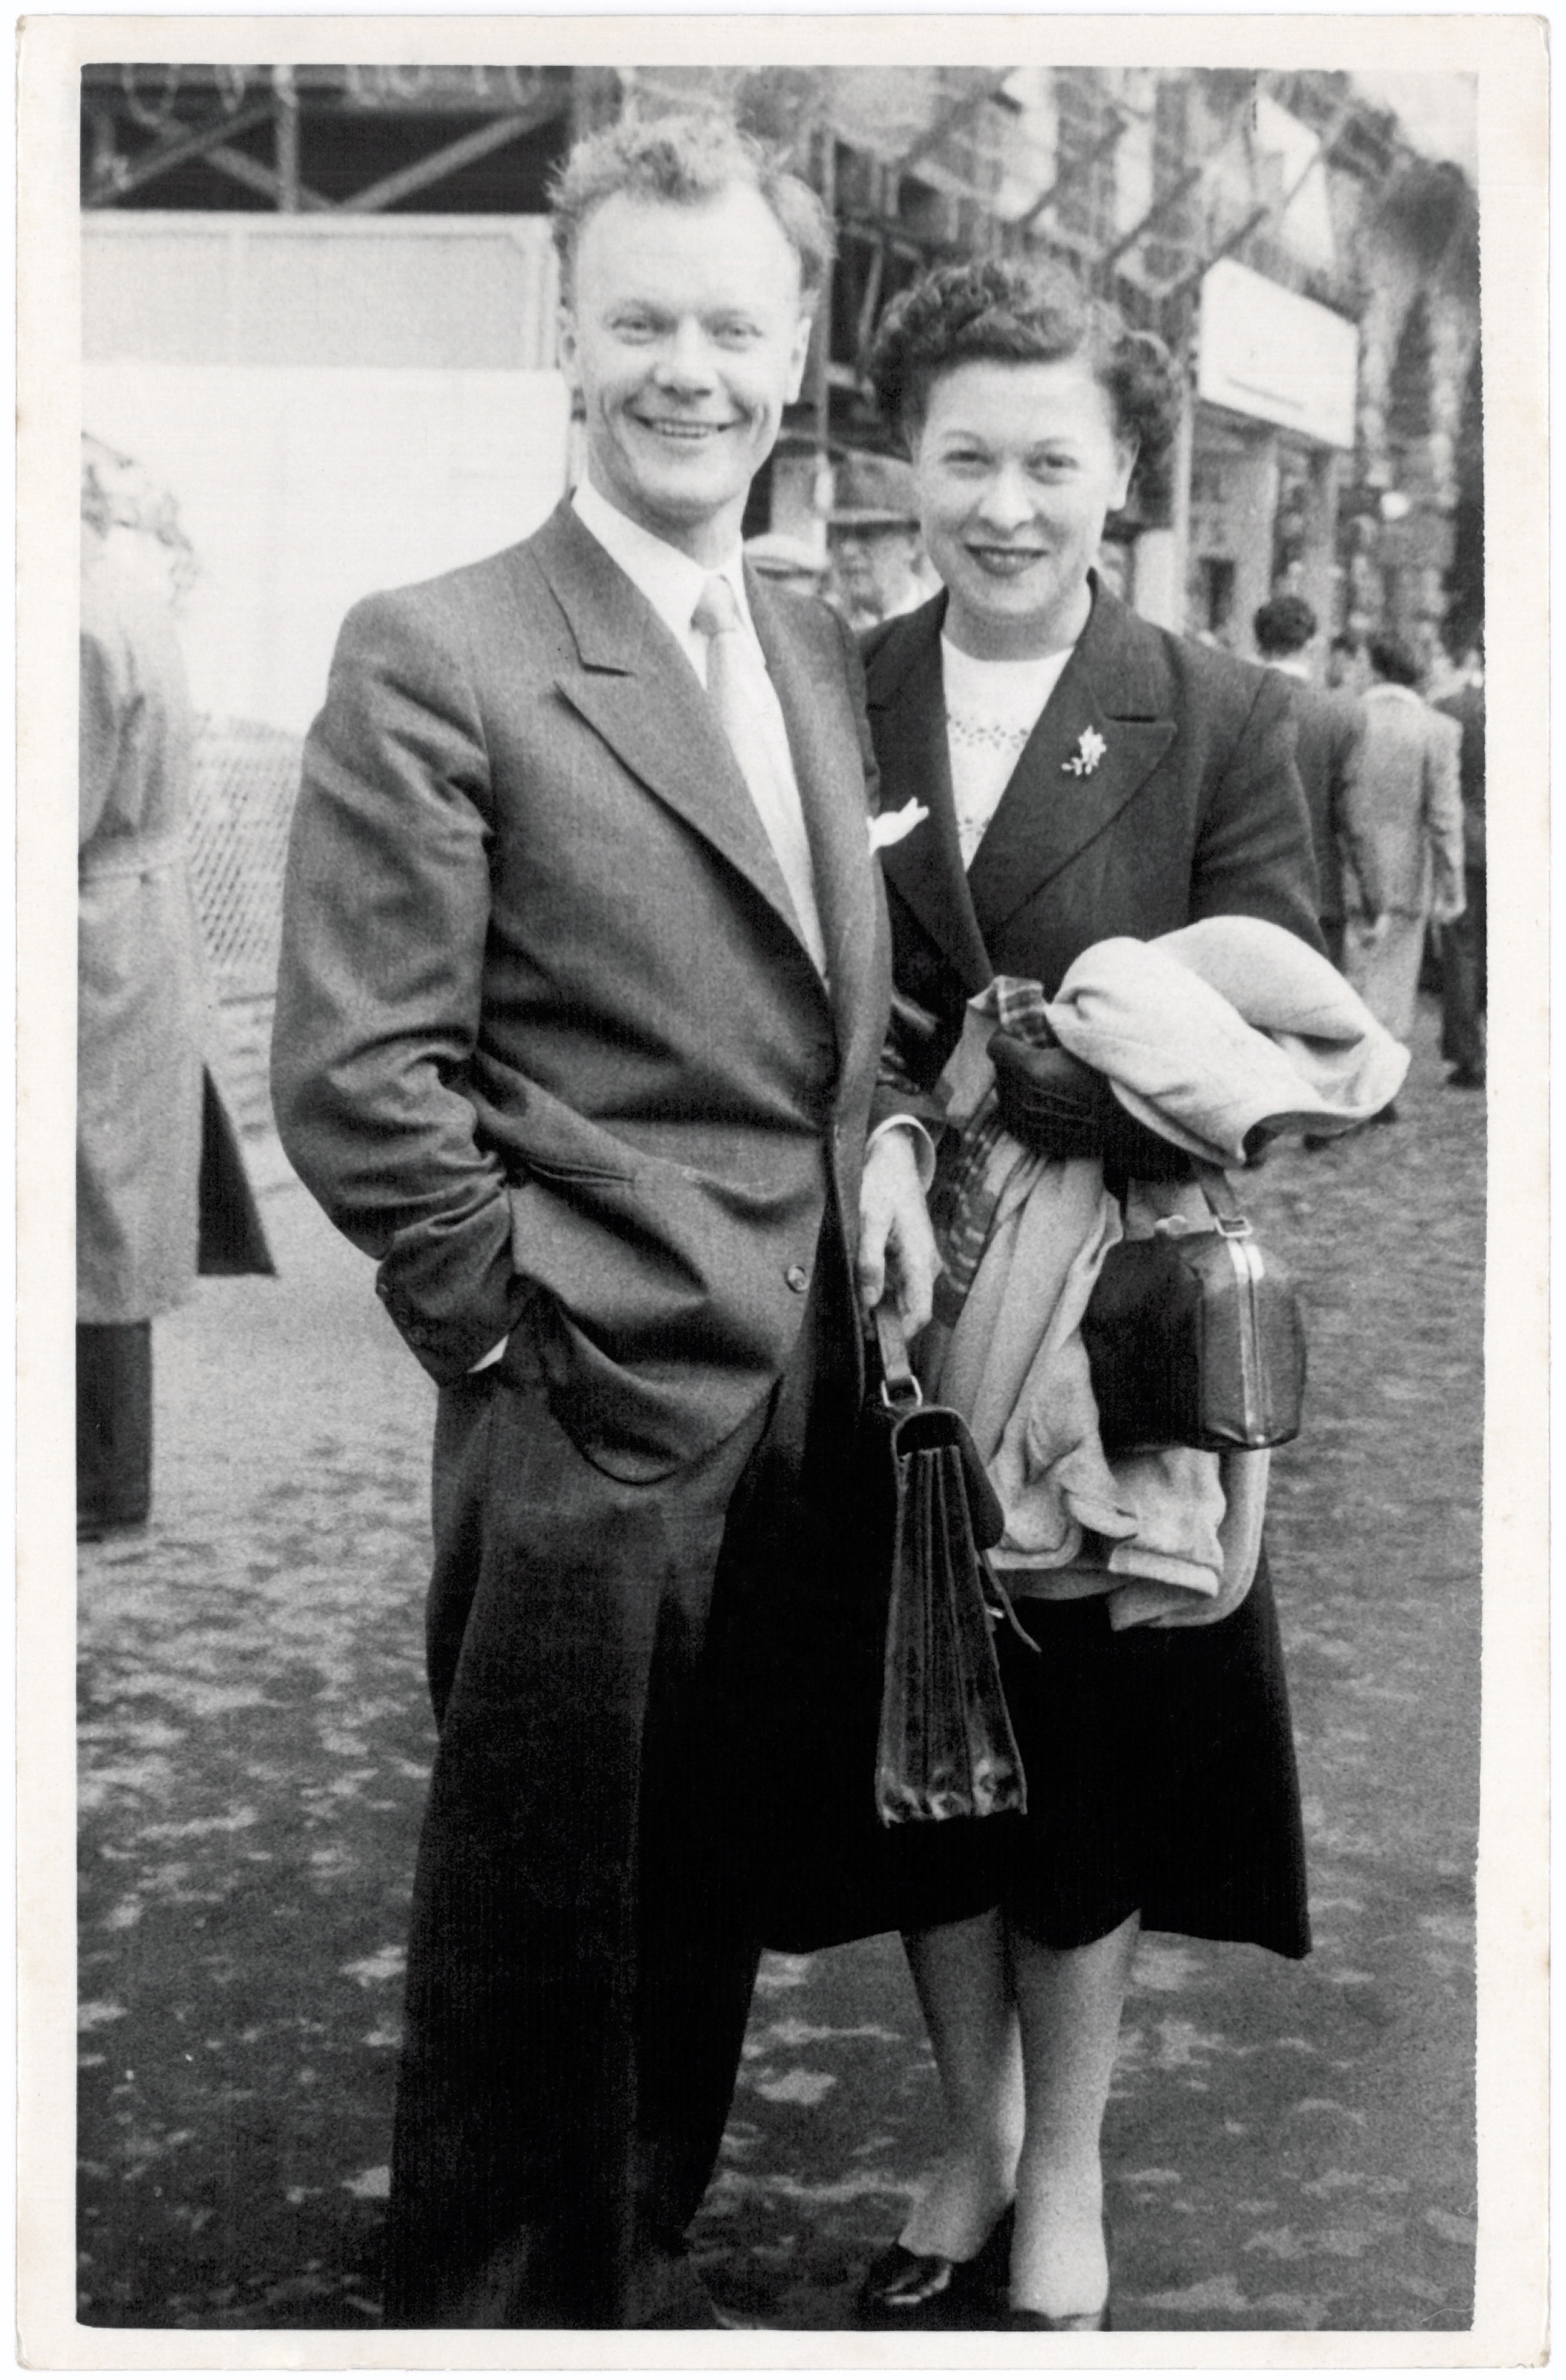
\includegraphics[width=0.45\textwidth]{photos/tony-and-madge3.jpg}\label{tony-and-madge3}}
    } &
    \subfloat[Bryanston (1980).]{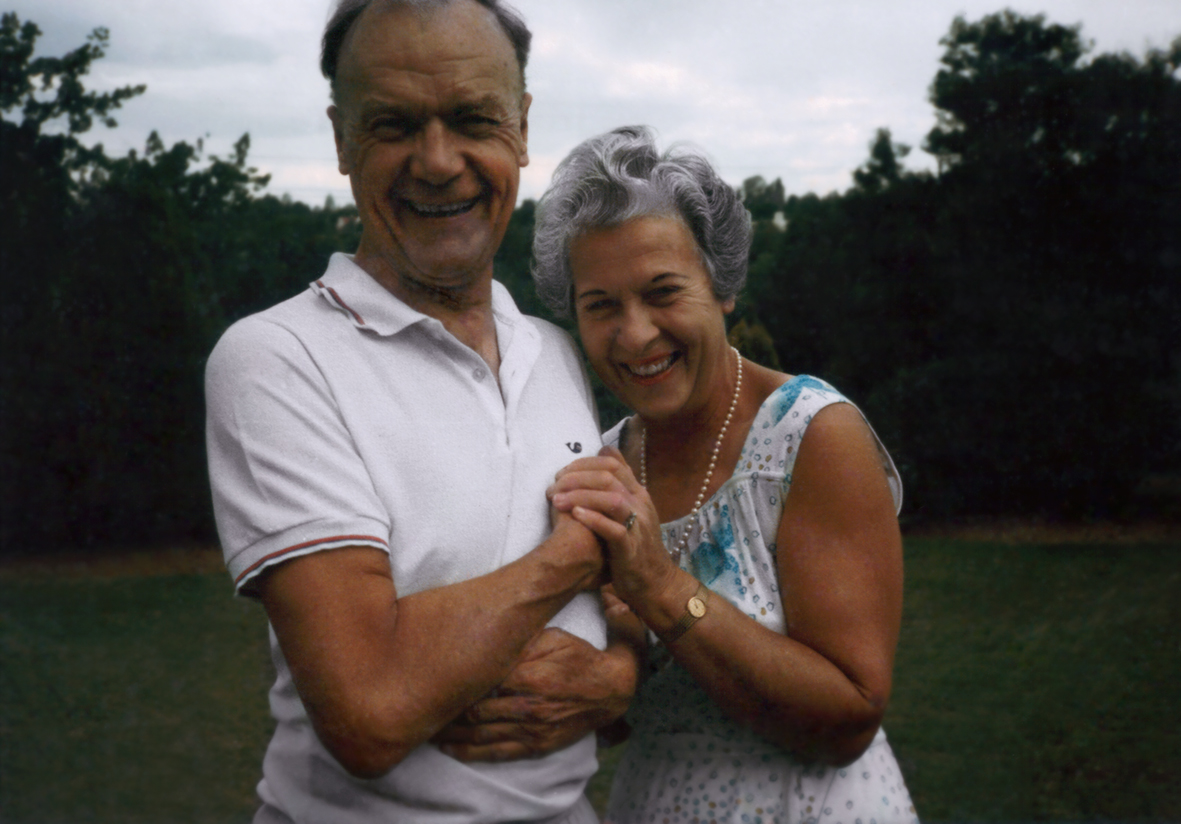
\includegraphics[width=0.45\textwidth]{photos/tony-and-madge2.jpg}\label{tony-and-madge2}}
    \\
    &
    \subfloat[Johannesburg (1982).]{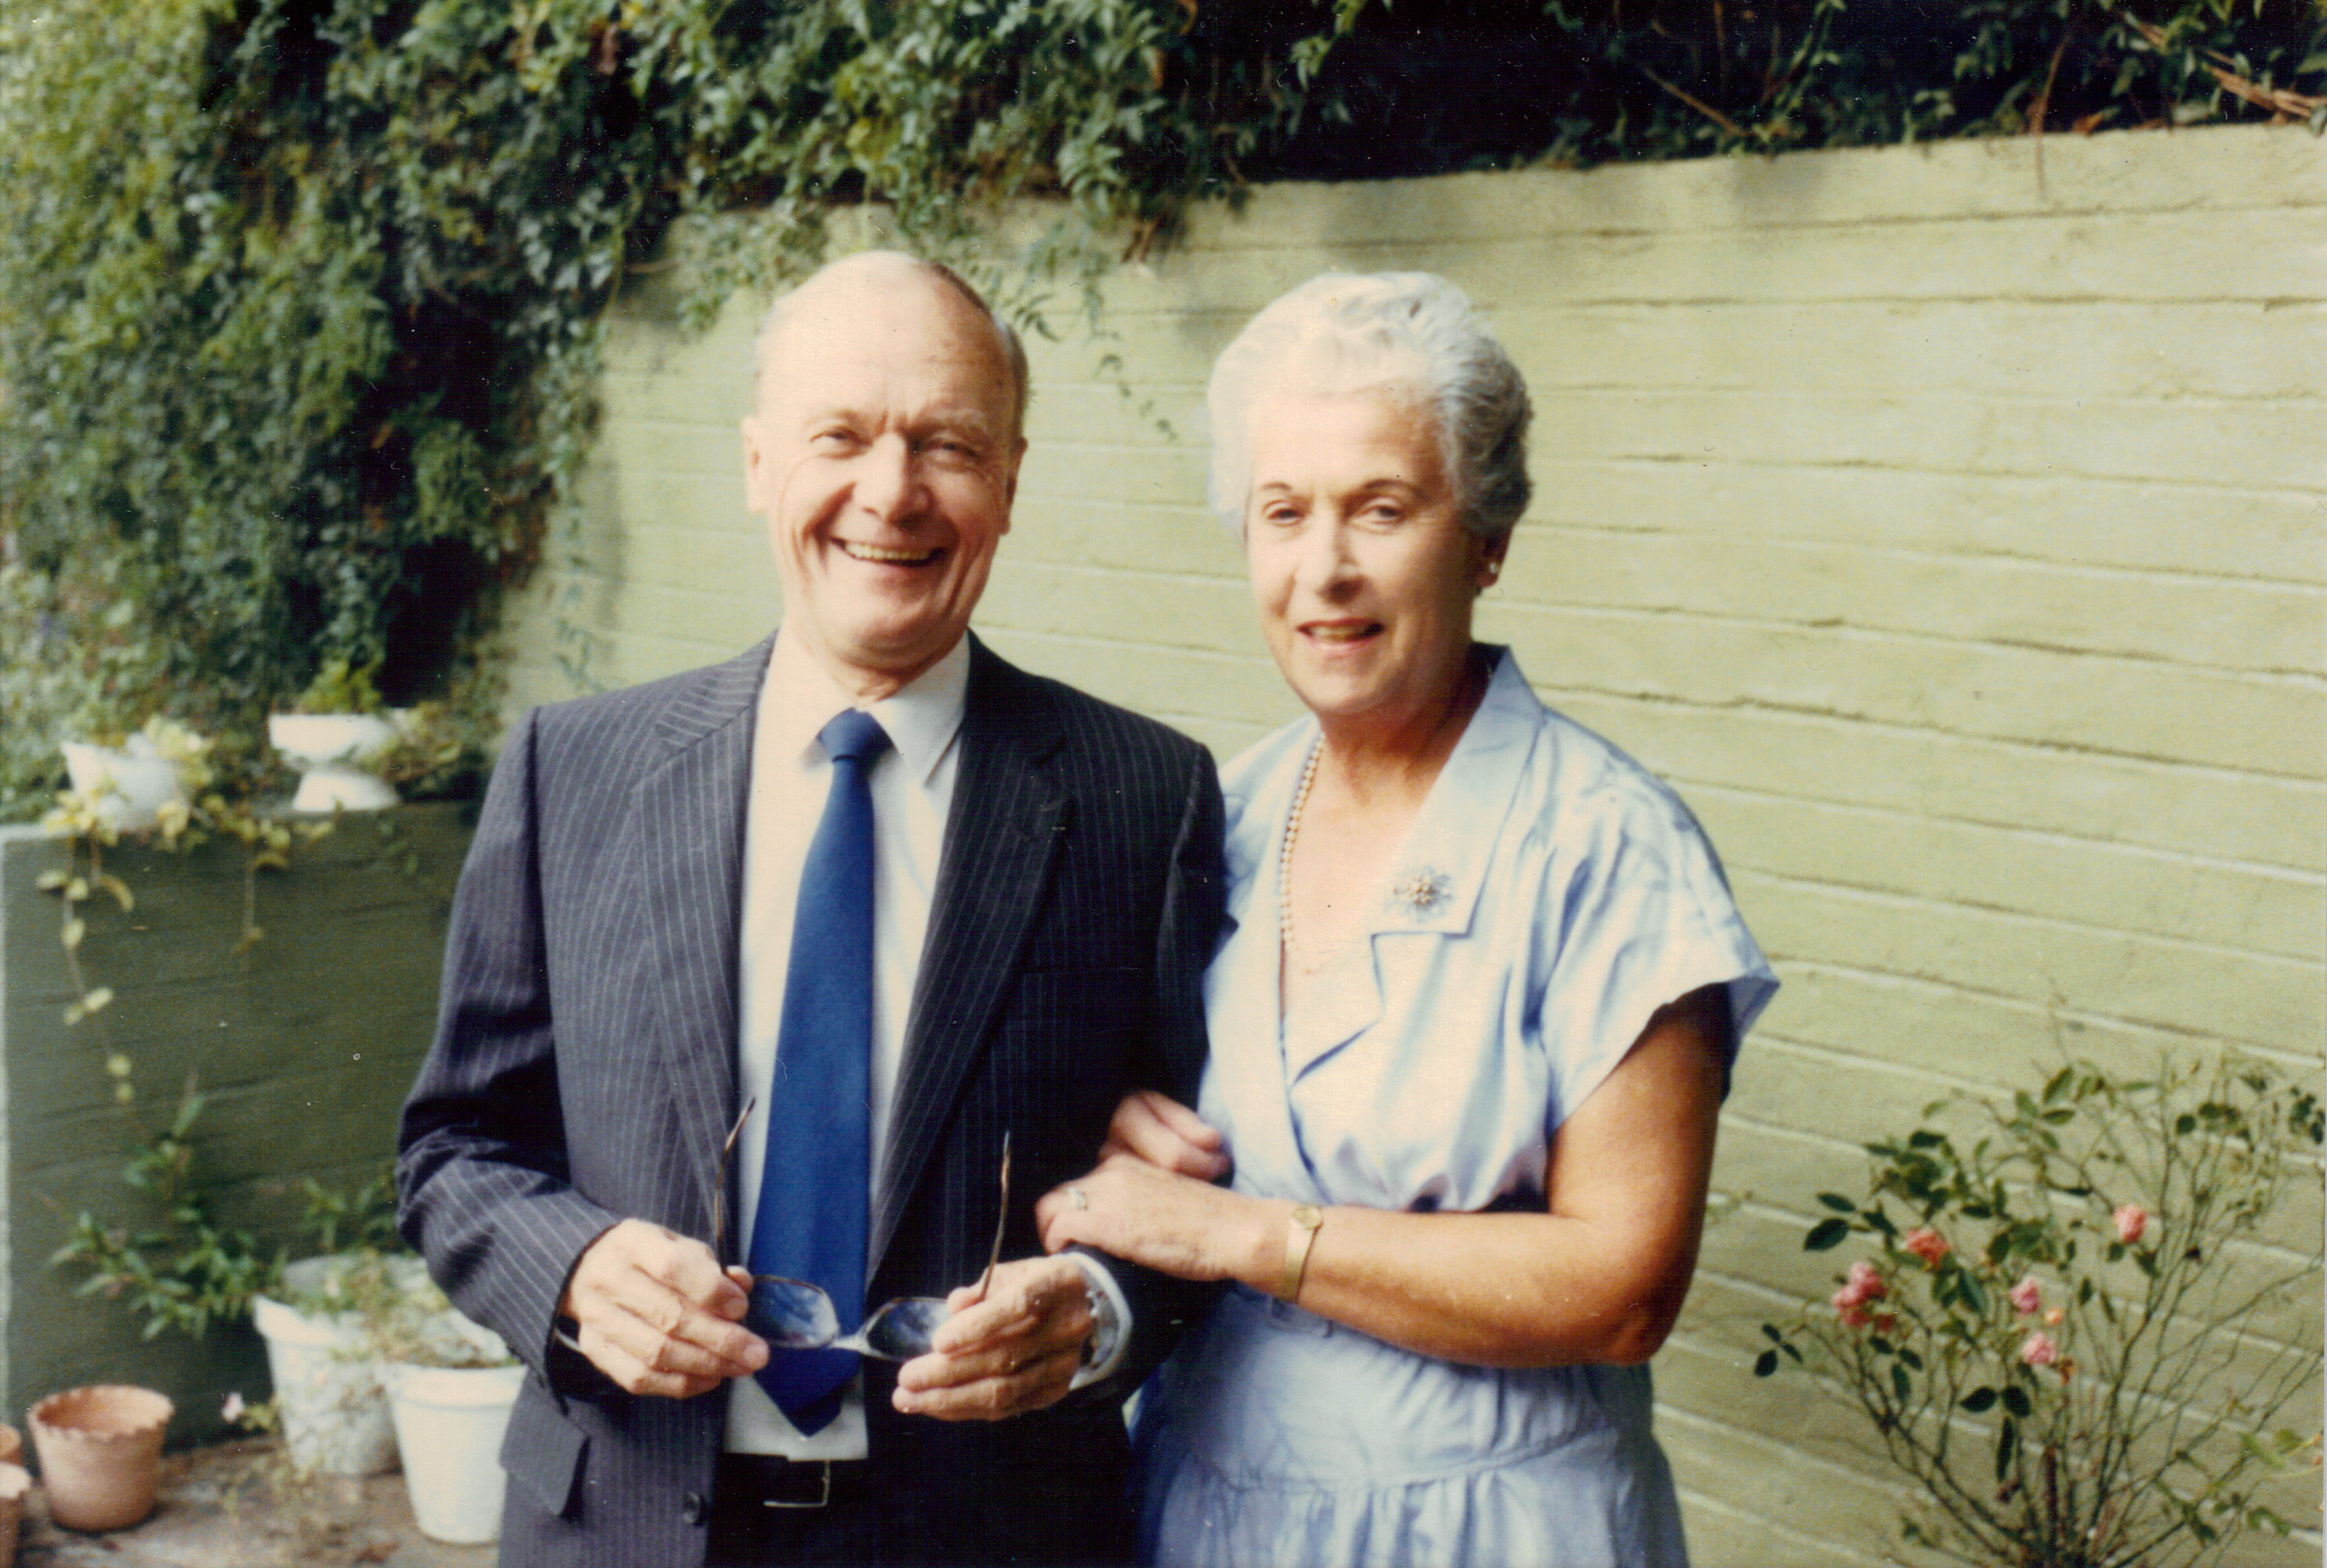
\includegraphics[width=0.45\textwidth]{photos/tony-and-madge.jpg}\label{tony-and-madge}}
    \\
  \end{tabular}
  \caption{Tony and Madge through the years.}
\end{figure}


\chapter{Turkey}

After a short while there, we flew to Turkey with a night stop in
Rome. Again we were on the Viking plane which made so much noise it
was impossible to talk! Onto Athens and Istanbul and again the train
journey overnight to Ankara.

This train (thirteen hours between Istanbul and Ankara) was to have a
lasting horrible memory for me. On a trip four years later I suffered
a miscarriage during the night and had to be ``seen to'' on
arrival. The German woman doctor was brutal and administered treatment
without an anaesthetic and Tony, poor lad, had to be with me but he
was stoic as usual. I had two more miscarriages before I produced
Elizabeth. That was after seven years. What a triumph!

There was such a lovely welcome. Tony had been there for three years
and was well-known to hoteliers, restaurant owners and staff and, of
course, the company people too.

We had to find somewhere to live but, for a short time stayed in the
Park hotel. All very strange and different.

One evening I had a panic attack! Tony had promised to take me for
dinner early and I was ready at six. I waited and waited and stood by
the window looking down on the street and realized that there was no
one who would want to talk to me and no one to whom I could talk to
not knowing enough of the language, I thought ``My mother was right, I
don't know this man, where is he?'' Tony came at 10pm having worked
until then, all was well but over the years I often wondered why it
was so impossible to pick up a telephone and tell me he would be
late. Years later in Nigeria I was waiting and the phone rang -- I
said ``Gee, I'm hungry'' and a well-bred voice said ``I'm so sorry to
hear that, Mrs. Bray.'' It was the permanent secretary to the
P~\&~T.\footnote{Post and Telegraph.} Such a nice man he never
mentioned my faux pas!

We found the time to explore Istanbul and I was enchanted with
everything there -- the cobble street, the Pera-Palace Hotel, the
Mosques and museums, the whole atmosphere was magic (the covered
market too). We often returned to Istanbul from Ankara. One evening we
went for dinner to the Park Hotel where a small orchestra played -- we
requested \textit{Amame Ecore} and always afterwards when we arrived
they would break off what they were playing and play our
tune. Romantic stuff!

Came the time to leave Istanbul for Tony had finished the work he had
to do there. He was based in Ankara and so we had to find somewhere to
live. There were several really old houses but we settled on one which
had only one serious defect -- there was a gap right across the centre
of the lounge; we learned to live with it. It could have been
dangerous but we never fell! I tried to teach Tony to dance although
he was not interested and the ``gap'' did not help so we usually
finished up laughing hysterically -- this to be followed up by some
glorious love-making!

The kitchen was primitive and so was the plumbing. Melon pips would
come down a drain right into our kitchen. Luckily we were able to
sweep the pips into another drain (I never could understand why the
two drains did not meet)!

It was dreadfully cold up on the Anatolian Plateau. We had a wood
stove in the lounge and a caretaker would come each day to clean it
out and light it. I was learning the language very slowly but enough
to take me shopping and I would practice the words of what I had to
buy as I walked down to the shops. One was not expected to pay the
prices asked but to make a pazalik (bargaining) after a while I was
brave enough to do that! I did not know it then but very many of the
Turkish people could speak English but held back. I enjoyed our little
flat but very soon I went with Tony to see other more primitive parts
of Turkey. This was an eye-opener to say the least! And I think an eye
opener too to some of the natives for I must have looked like someone
out of outer space. Turkey is a Muslim country and the women cover
their heads and faces. I was never apprehended for not covering my
head. In the winter I was dressed in slacks, overcoat, scarf and
gloves and boots -- but no hat.

The GEC telephone equipment (new, pristine and shining) would be
housed in what looked like a hovel but there were good technicians who
cared for the equipment in these repeater stations. At every town or
village Tony was greeted like a long lost cousin by these wonderful
country people and they seemed to enjoy meeting me too.

One experience I shall never forget was being invited into a small
house for morning coffee. I think that seeing me was due to
curiosity. I was set up on a dais in quite a small room where there
were no chairs or tables but pretty cushions to sit on -- half the
women of the village were there bringing babies and small
children. Everyone fitted into the room. By this time I knew enough of
the language and the questions came:

``Do you like our country?'' -- ``Yes.''

``Do you like our food?'' -- ``Yes.''

``Is England like our country'' -- ``No, it's different, but I love
Turkey.'' (tact)

``How long have you been married?'' -- ``Eighteen months!'' -- ``Then
you should have 2 children!''

It would not have been the moment to explain that one could postpone
this event so I just called on Allah and said ``Allah versin'' (Allah
will give) or ``Inshallah'' (Allah will know the moment). Phew!  This
was accepted. We had delightful sweetreats and Turkish coffee. I felt
very pleased and proud of my ``press conference''!

Staying in a village ``hotel'' was something else. There was but one
wash basin for the entire complement of visitors. And I had to queue
up with other ``guests'' (mostly men) to wash my face and hands
only. My mother would have been horrified but nothing was going to
daunt me then. Tony would not have wanted a grizzling wife!

It was a relief to reach another hotel sometimes and to have a welcome
bath. One place we stayed in was built of cow manure and
whitewashed. Snakes could come out of the ceiling but I never saw
one. Oh! We had to ask for clean sheets for they were seldom
changed. What a paradise to return to Ankara or Istanbul and savour
the clean cool sheets!

There were lovely things to have on these trips and I will never
forget the huge peaches of Bursa or the melons of Diyarbakir. This
latter place was surrounded by a thick, thick wall where there were
thousands of scorpions -- school children would collect them and bring
them, dead or alive and be paid handsomely for each one. Hospitality,
scenery and sunsets played a large part in these travels and one
always remembers the nice aspects.

It was nice to return to our funny little flat but often for a short
time for our travels would begin again and Tony would have more
installation work to do. It was good to get away sometimes from the
hopelessly crippled beggars who would come knocking at the door. It
was common practice for babies to be maimed at birth in order to be
able to spend their lives begging. I am ashamed that I would just slam
the door but it was often a very awful sight.

Once whilst I was waiting for Tony in some public place in Istanbul, I
was sitting opposite a man who kept staring at me. The Turks are known
for this habit but I objected and poked my tongue out at him. Tony was
furious -- I could have got a knife in my back!

The time came for Tony's contract in Turkey to finish and we had a
final tour to Istanbul and Izmir (Smyrna in the Bible) this was
intensely interesting because we had the opportunity to go to Ephesus
(Efus in the Bible) from Izmir. There is too much history to be told
here. It is a always wonderful experience to stand still in historical
and ancient surroundings and think of the amount of history which has
taken place there. Several of St. Paul’s journeys were made in Turkey
and it is daunting to realise that the very ground one is standing on
is still the same as it was centuries before. How lucky I am to have
seen all of this and how lucky to be able to remember it. Goodbye
Turkey -- I shall never forget you!


\chapter{Elizabeth \& Richard}

Even before she was born, Elizabeth showed a tenacity and strength of
purpose. For, in spite of a set back at Christmas~1959, she hung on
and was determined to be born which indeed she was in July~1960. She
was a beautiful and contented child and we delighted in her.

There is always another Mother Grundy lurking -- someone who likes to
bring criticism and unhappiness into another person's life. I met such
a person when I was out pushing Elizabeth in her pram. She said ``That
child is sucking her thumb because she lacks something in her life --
probably love''. To which I replied ``Madam, we have waited 7~years
for this child and she lacks nothing, least of all love, except
perhaps a carpet in her bedroom and I am quite sure she is unaware of
that.''

% We had arrived back from Turkey in 1956 and were quite settled into
% our lovely house in Leamington Spa when Tony was offered a top posting
% with the GEC in Nigeria.

We had arrived back from Turkey in 1956. Returning to England from
Turkey was very different and the five years we spent there had their
difficulties. Tony had ``almost'' a gastric ulcer according to the
doctor. He did not settle down to factory life and felt inhibited by
the set hours. He had been used to travelling long distance and having
quite an adventurous way of life.

We built a house in Leamington Spa close to the GEC in Coventry. We
bought new furniture and developed the garden (well I did). It was a
useful time for this when Tony went off to Finland for two business
trips -- one of three months and one of ten weeks. I took off the turf
and then dug deep and grew marvelous vegetables (and raspberries and
almost killed Tony with the acid). Nothing to it. Of course the ground
had been a horse paddock and so was very well manured.

All this exercise had to stop when I became pregnant with Elizabeth. I
had to be extra careful as I had had two miscarriages. She arrived in
July 1960. No one but me had ever had a baby! We had had to wait for
seven years.

We were quite settled into our lovely house in Leamington Spa when
Tony was offered a top posting with the GEC in Nigeria.

He had to undergo certain tests and the doctor who pronounced him fit
said ``I have bad news for you, old chap -- you will be able to go to
Nigeria.'' We both had to have injections for typhoid, TB, yellow
fever, etc. Our house had to be sold and the furniture put into
storage; I was so upset that I could not watch the removal van drive
away.

Tony flew on ahead to Lagos but Elizabeth and I made the 13~day trip
by sea. My dad drove us and the 2 grandmothers to Liverpool to embark
on the ship.

They were heartbroken at the thought of our being taken to that
``God-forsaken place'' and I could not help feeling sorry for
them. Tony's father had passed away and never saw his
granddaughter. He would have been terribly upset by this parting.

March is not the best time of the year for crossing the Bay of Biscay
for the sea is very turbulent. So much so that I succumbed to
sea-sickness and felt very ill for 5~days.

Once more, Elizabeth displayed her stoicism by marching up the deck as
if in a straight line. I had to carry on; she loved her food and I had
to carry her up 2~flights of stairs to the childrens' restaurant --
hopefully finding a place for her by the door so that I could exit
quickly to the bathroom!

Once we had passed the Canary Islands I felt much better and was able
to enjoy the wonderful food and activities. One can understand the
temptation of shipboard romances. The whole atmosphere was wonderful
-- the incredible inky blue of the sea in the moonlight, the smooth
passage of the ship through the water after the awful turmoil, and the
constant playing of ``Moonriver'' over the sound system. I shall
always love that song (as I write this in September 2012, I hear that
Andy Williams, the composer, died yesterday; what a lovely song and
tune he left).

Apparently I ``waddled'' off the ship due to the good food. It was
great to see Tony again but oh! arriving in Lagos was like walking
into hot pea soup with the temperature and humidity at impossible
levels.

Never mind -- we were a family again.

Once we were accustomed to the climate, life became reasonably
enjoyable. For the 11~years we were in Nigeria we occupied the same
house; even when we went on leave, the house was always
``ours''. There was air-conditioning upstairs but we had to lose the
comfort of this many times due to the frequent electricity cuts --
sometimes up to 72~hours. Nigeria had gained independence in 1960 and,
inevitably, basic services failed.

Our house was one of 4 in a compound and in the grounds were the
servants quarters. In one of these lived a little black girl. She and
Elizabeth became good friends and they played together in our garden.

When she was 4, Elizabeth started attending St. Saviour's school. This
was a Church of England school attached to St. Saviour's church in
Lagos where the rector was Reverend Jim Payne; his wife, Dorothy Payne
was the headmistress of the little school.

All the teachers were expatriates and it was interesting to see pupils
of different nationalities attending the school. But the majority were
Nigerian because the government only allowed the school to function if
this were the case.

A mixture would turn up at one of the birthday parties and once, there
were 5~Nigerians. When I remarked on this, Elizabeth said ``Does it
matter?'' Of course not. Children do not notice colour.

Our house boy, Audu, from the northern Hausa tribe, was as efficient
in the garden as he was in the house. He and Elizabeth developed a
strong friendship. One day she brought home from school a ``Flame of
the Forest'' seed. Audu planted it in a tin and nurtured it until it
was ready to plant in the garden. It grew well and, eventually,
reached the height of the balcony. Unfortunately, a parasite plant had
wound itself around the tree. Before leaving for work one day Tony
said to our gardener -- Andrew -- ``Get that thing down,'' meaning the
parasite -- and he did, tree and all.

Audu and I were in a state when she came home from school. She cried a
lot (so did I) but she squared her shoulders and dried her tears and
said ``Well I must try again,'' which she did with Audu's help and
actually that tree grew taller and stronger than the first one (see
Pictures~\ref{elizabeth-with-audu} and \ref{elizabeth-with-gardener})!

In 1964 we granted Elizabeth's wish for a baby brother and Richard was
born. Because of a bad history I went back to my home town for the
birth, much to the disappointment of one Dr. Ogan in Lagos who tried
to persuade me to stay. He was such a nice man; he loved London and
the English people and also Australia and, only in the last 5~minutes
of the conversation, he would say ``I suppose we'd better take a look
at this baby.''

Elizabeth and I stayed with my parents in Anton and because of Tony's
stop-start attempts at getting some leave, we did not return to Lagos
until Richard was 6~months old (see Pictures~\ref{tony-family}).

% \begin{figure}
%   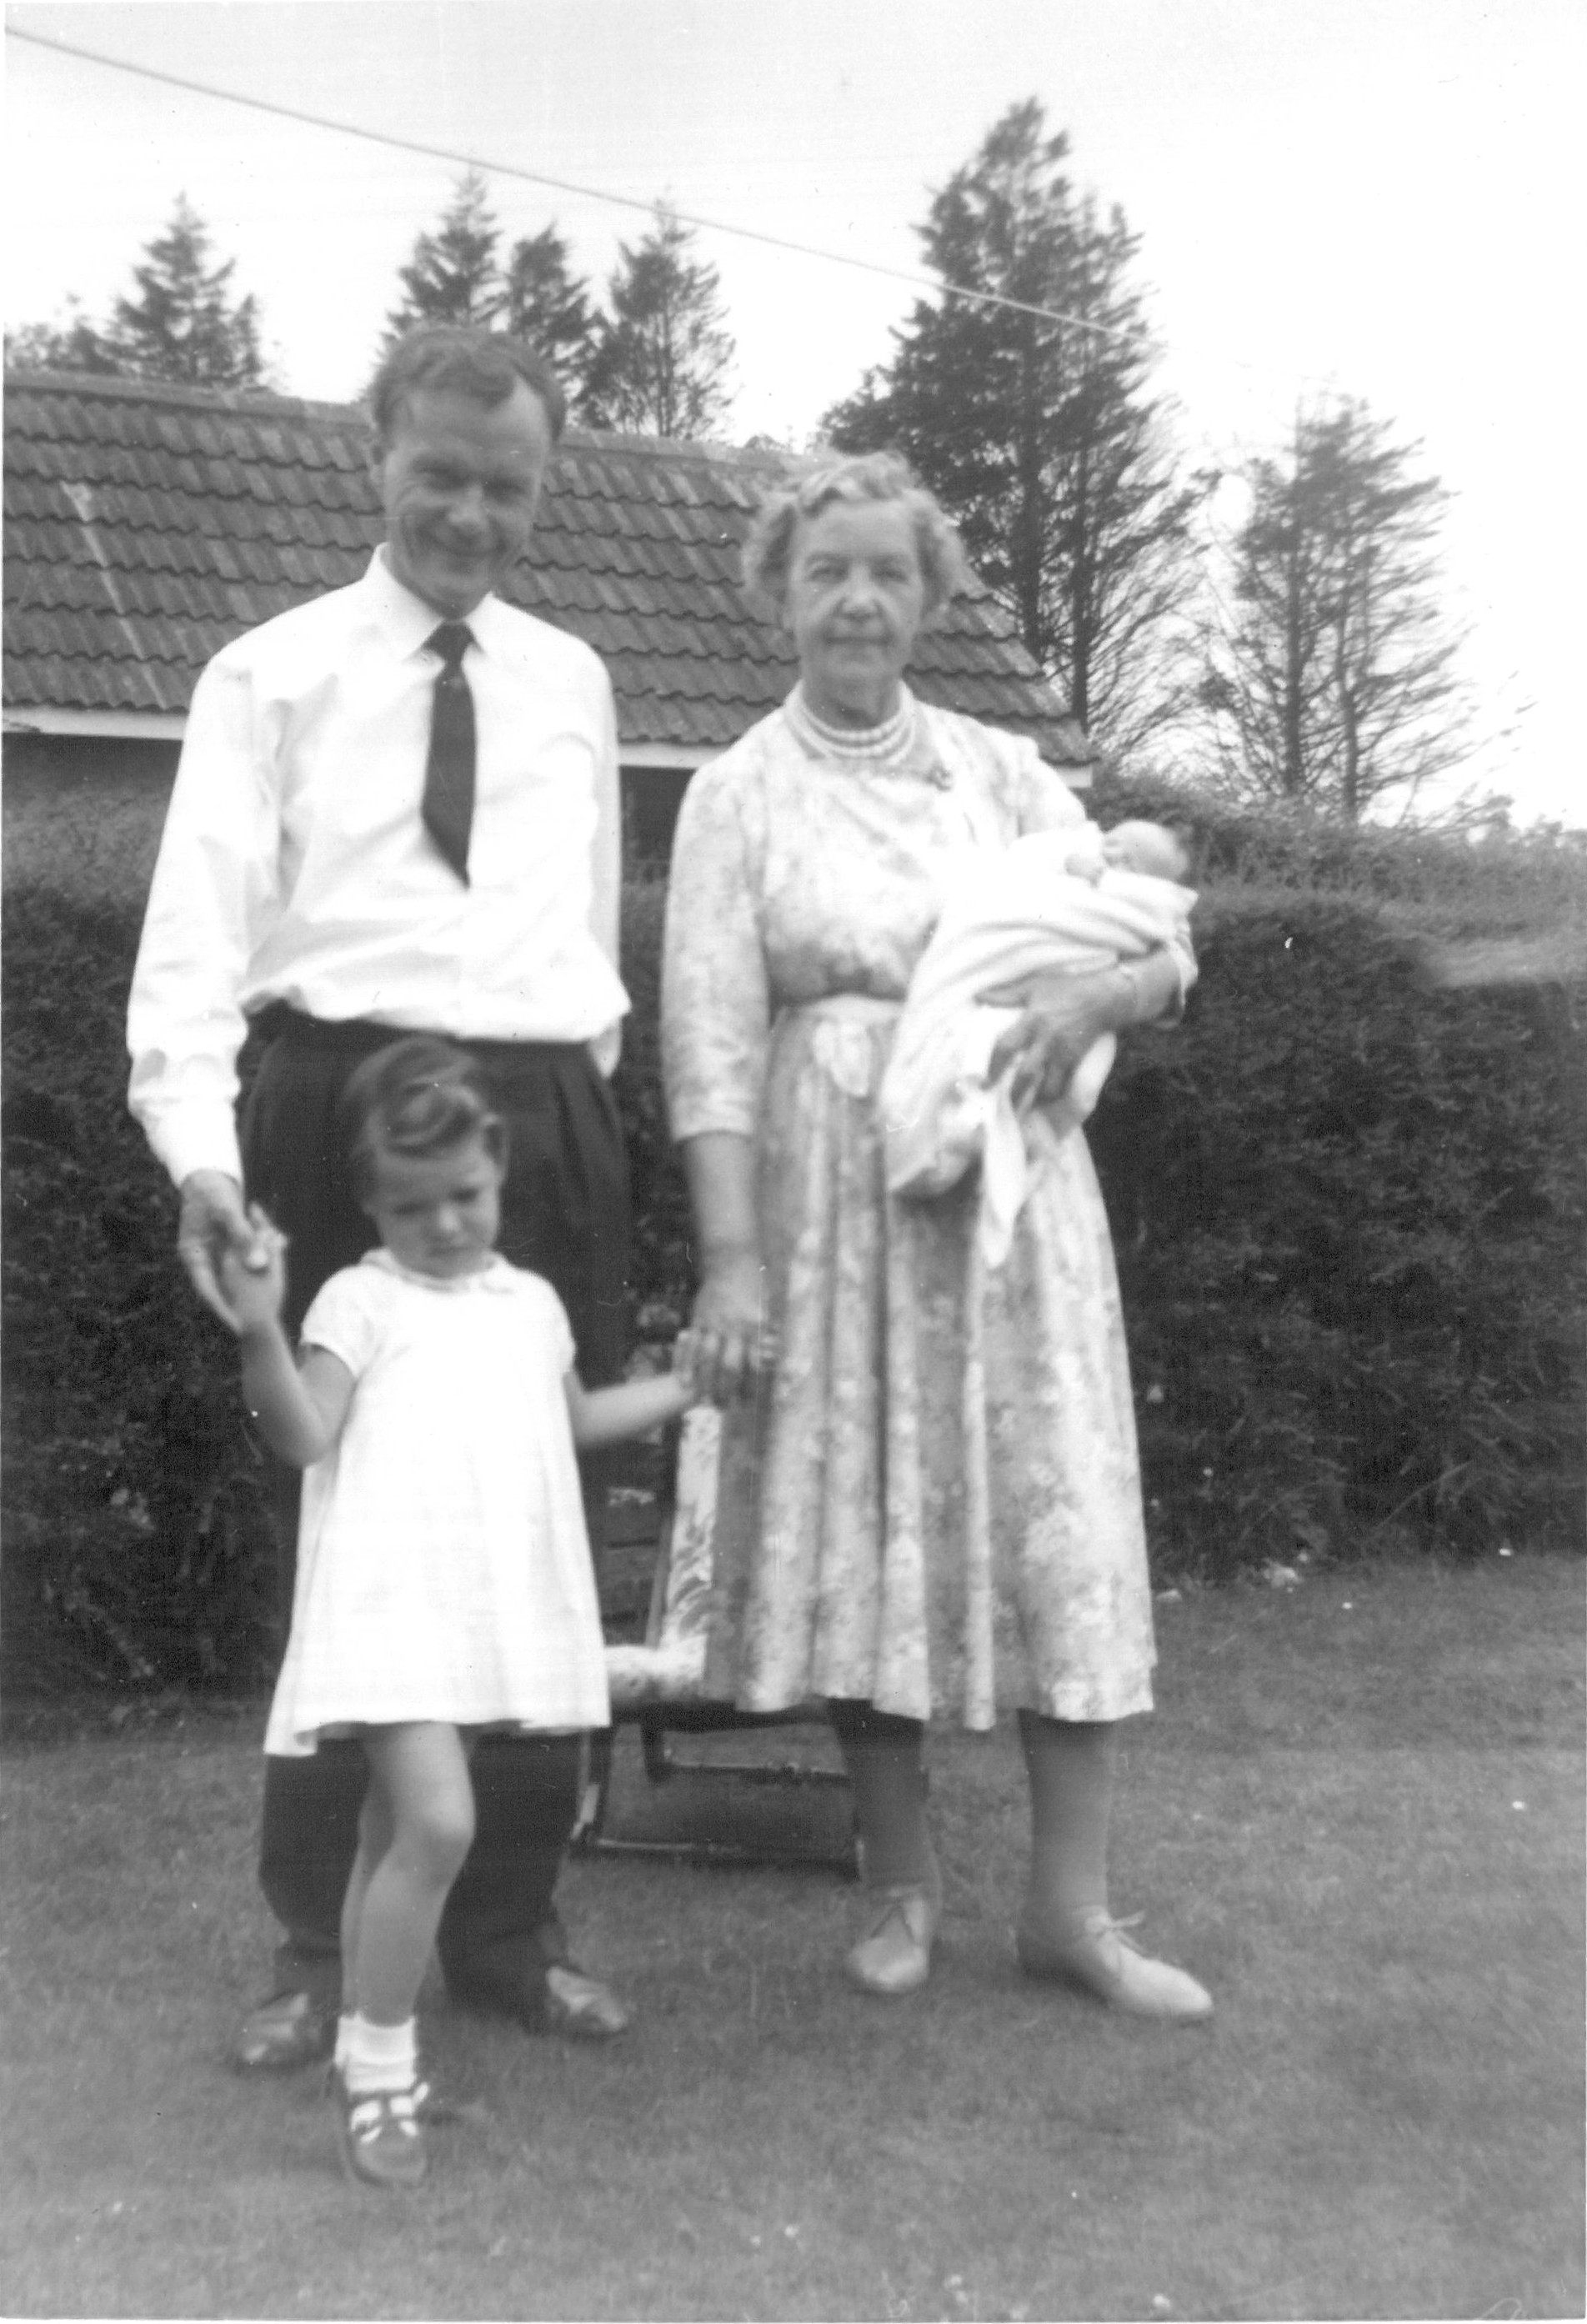
\includegraphics[width=\textwidth]{photos/tony-with-mother}
%   \caption{Tony with his mother, Elizabeth, and Richard (England, 1964).}
%   \label{tony-with-mother}
% \end{figure}

% \begin{figure}
%   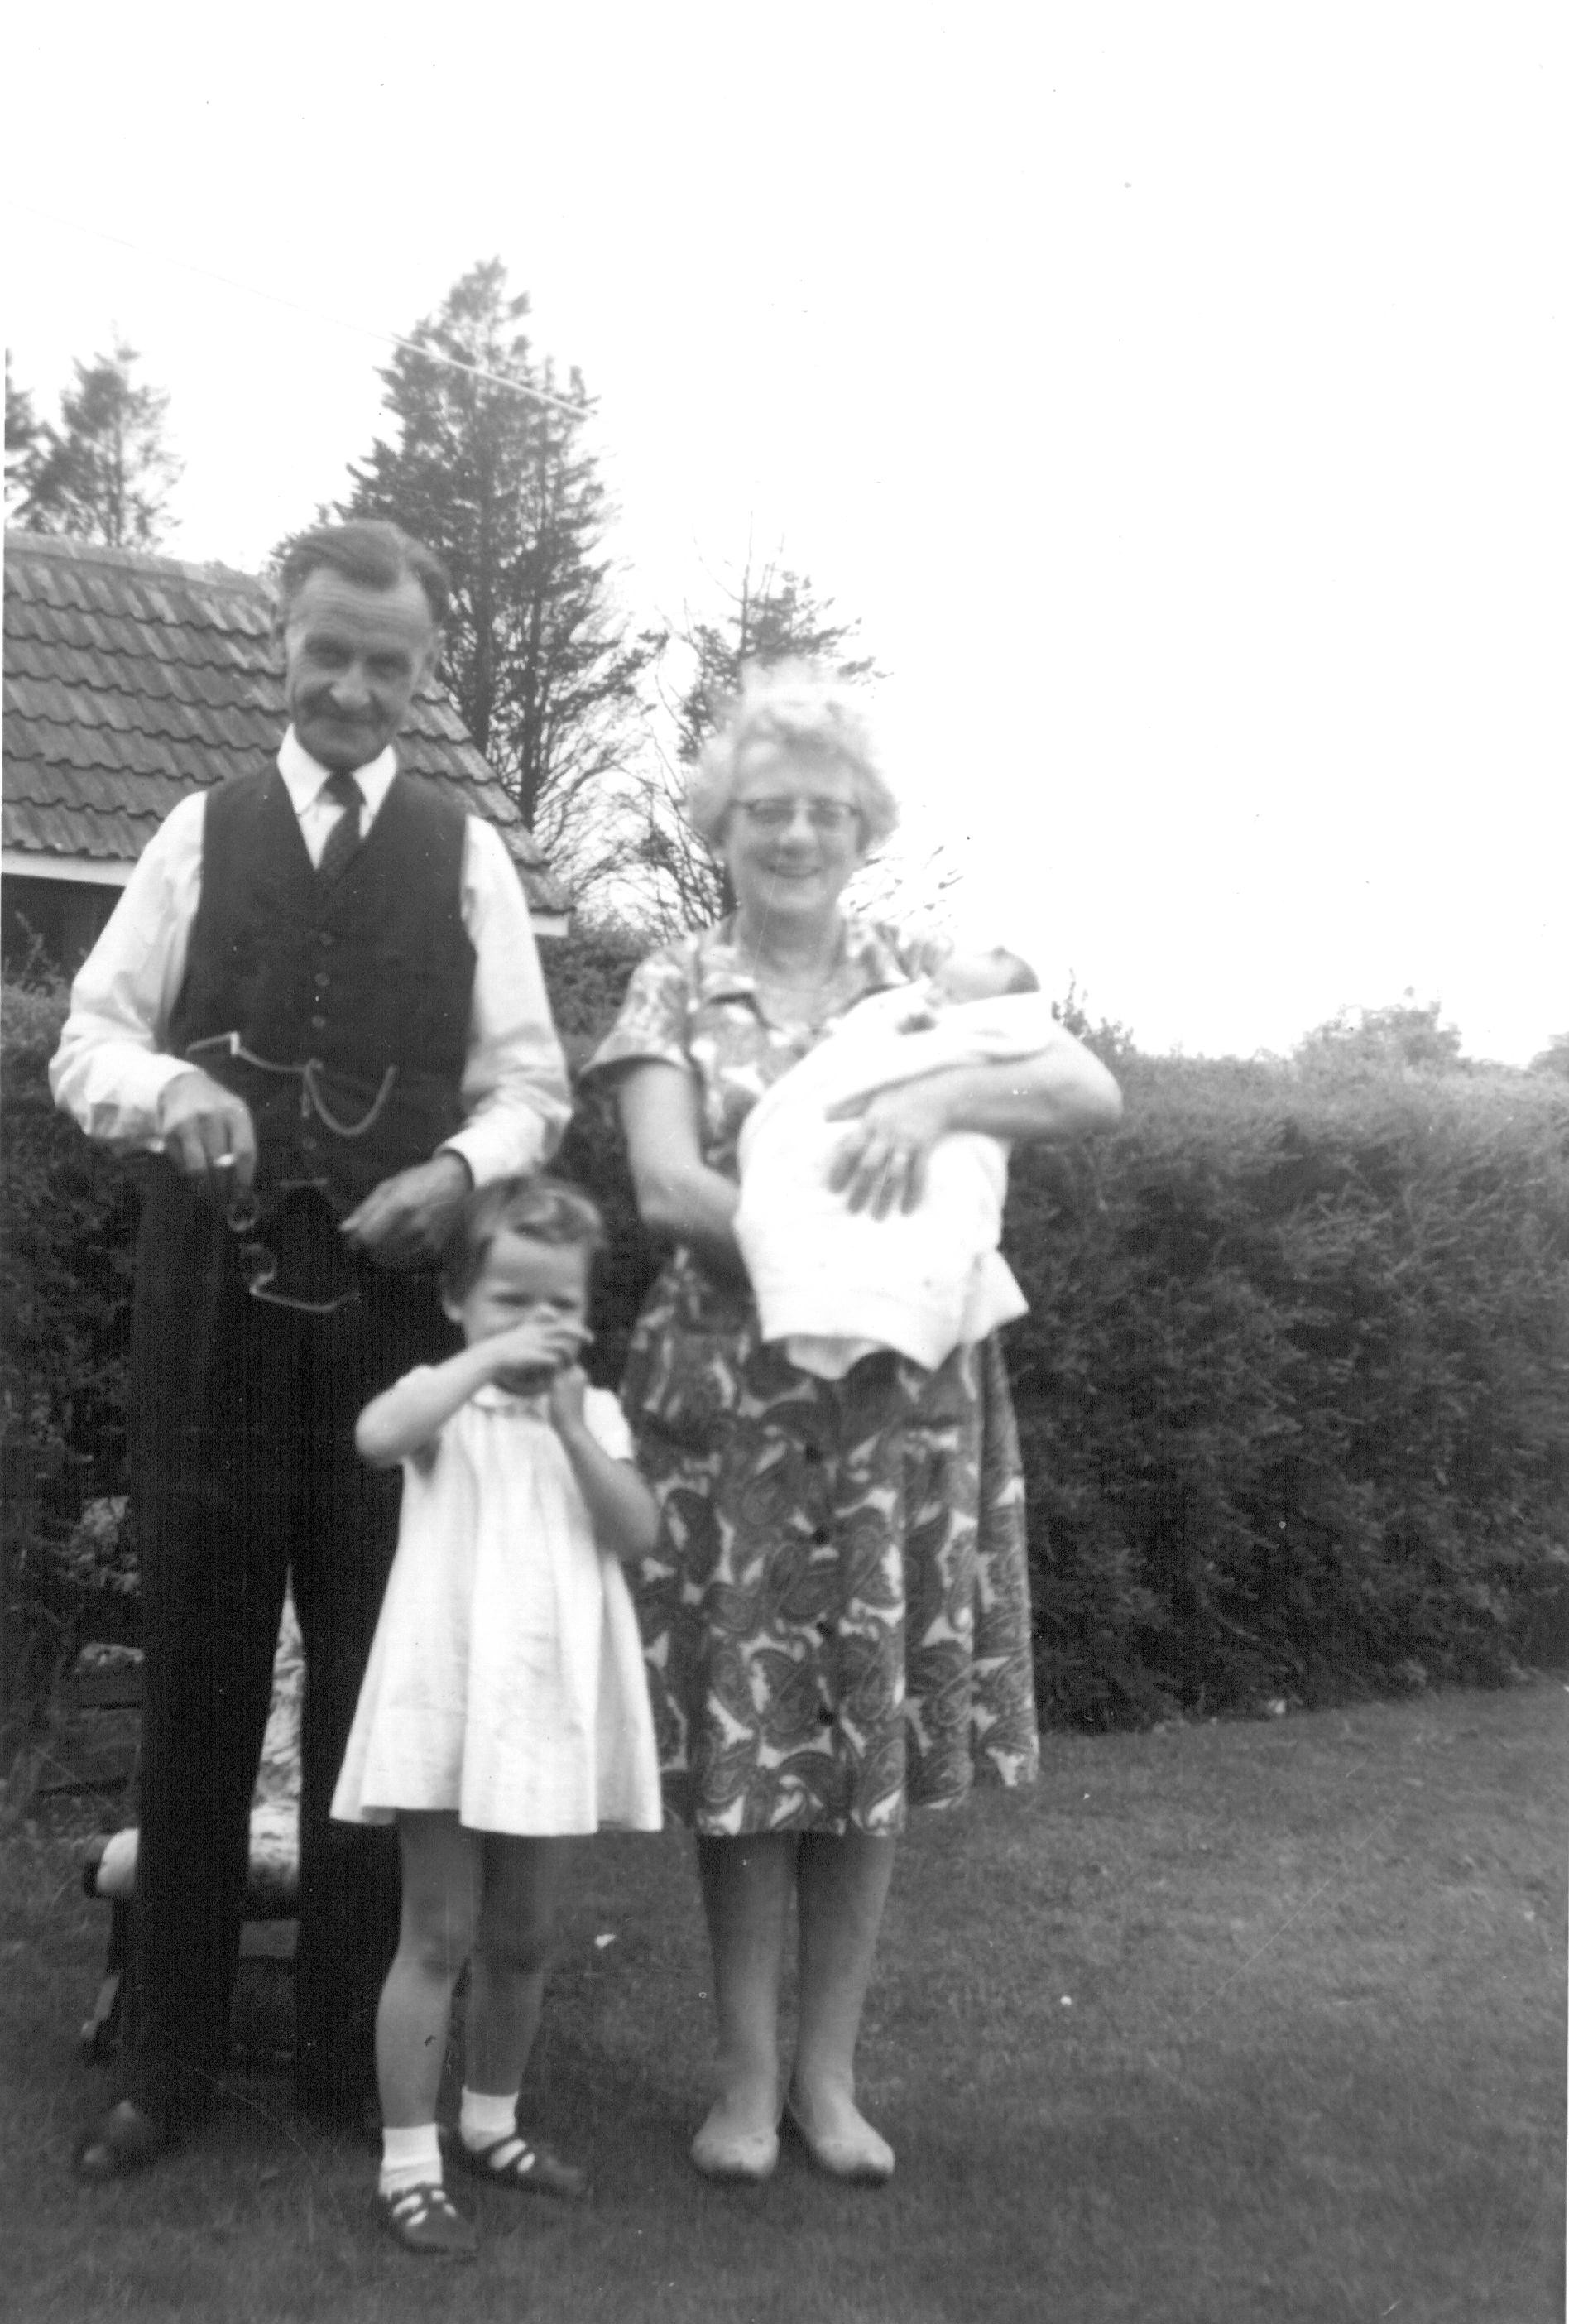
\includegraphics[width=0.9\textwidth]{photos/tony-parents}
%   \caption{Tony's mother and father with Elizabeth and Richard
%     (England, 1964).}
%   \label{tony-parents}
% \end{figure}

\begin{figure}
  \centering
  \begin{tabular}{cc}
    \subfloat[Madge's mother and father with Elizabeth and Richard.]{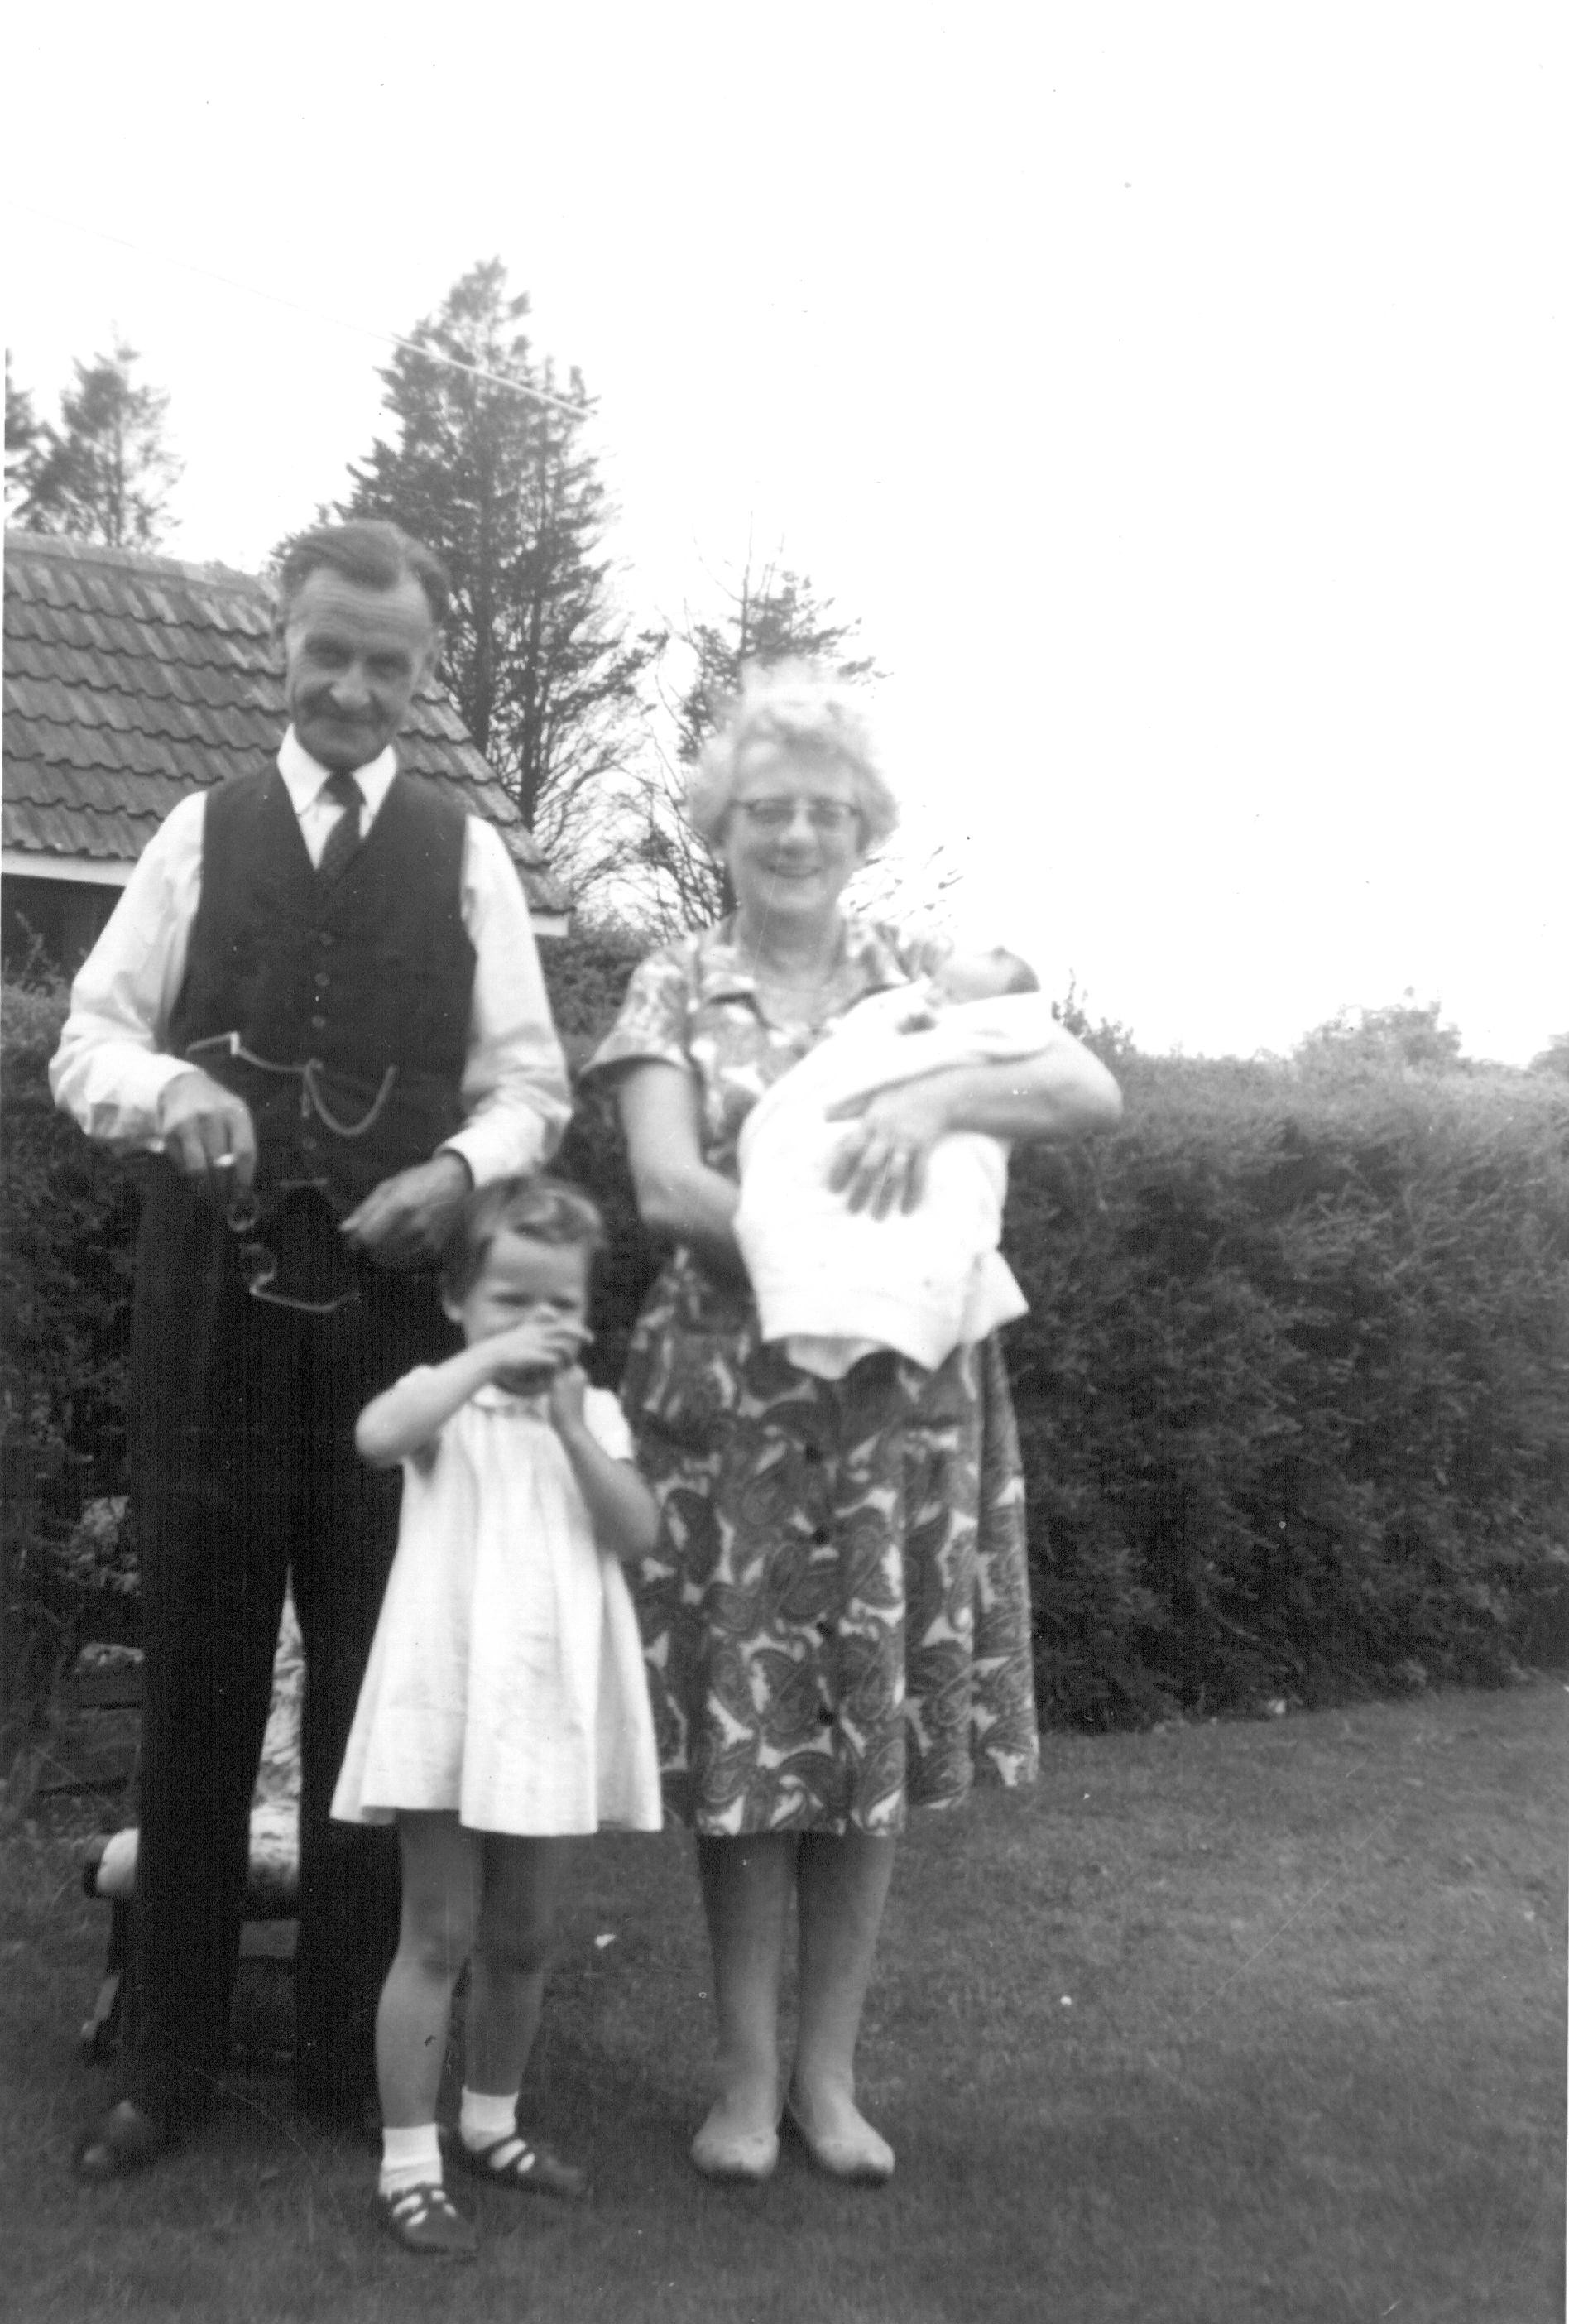
\includegraphics[width=0.45\textwidth]{photos/tony-parents.jpg}\label{tony-parents}}
    &
    \subfloat[Tony with his mother, Elizabeth, and Richard.]{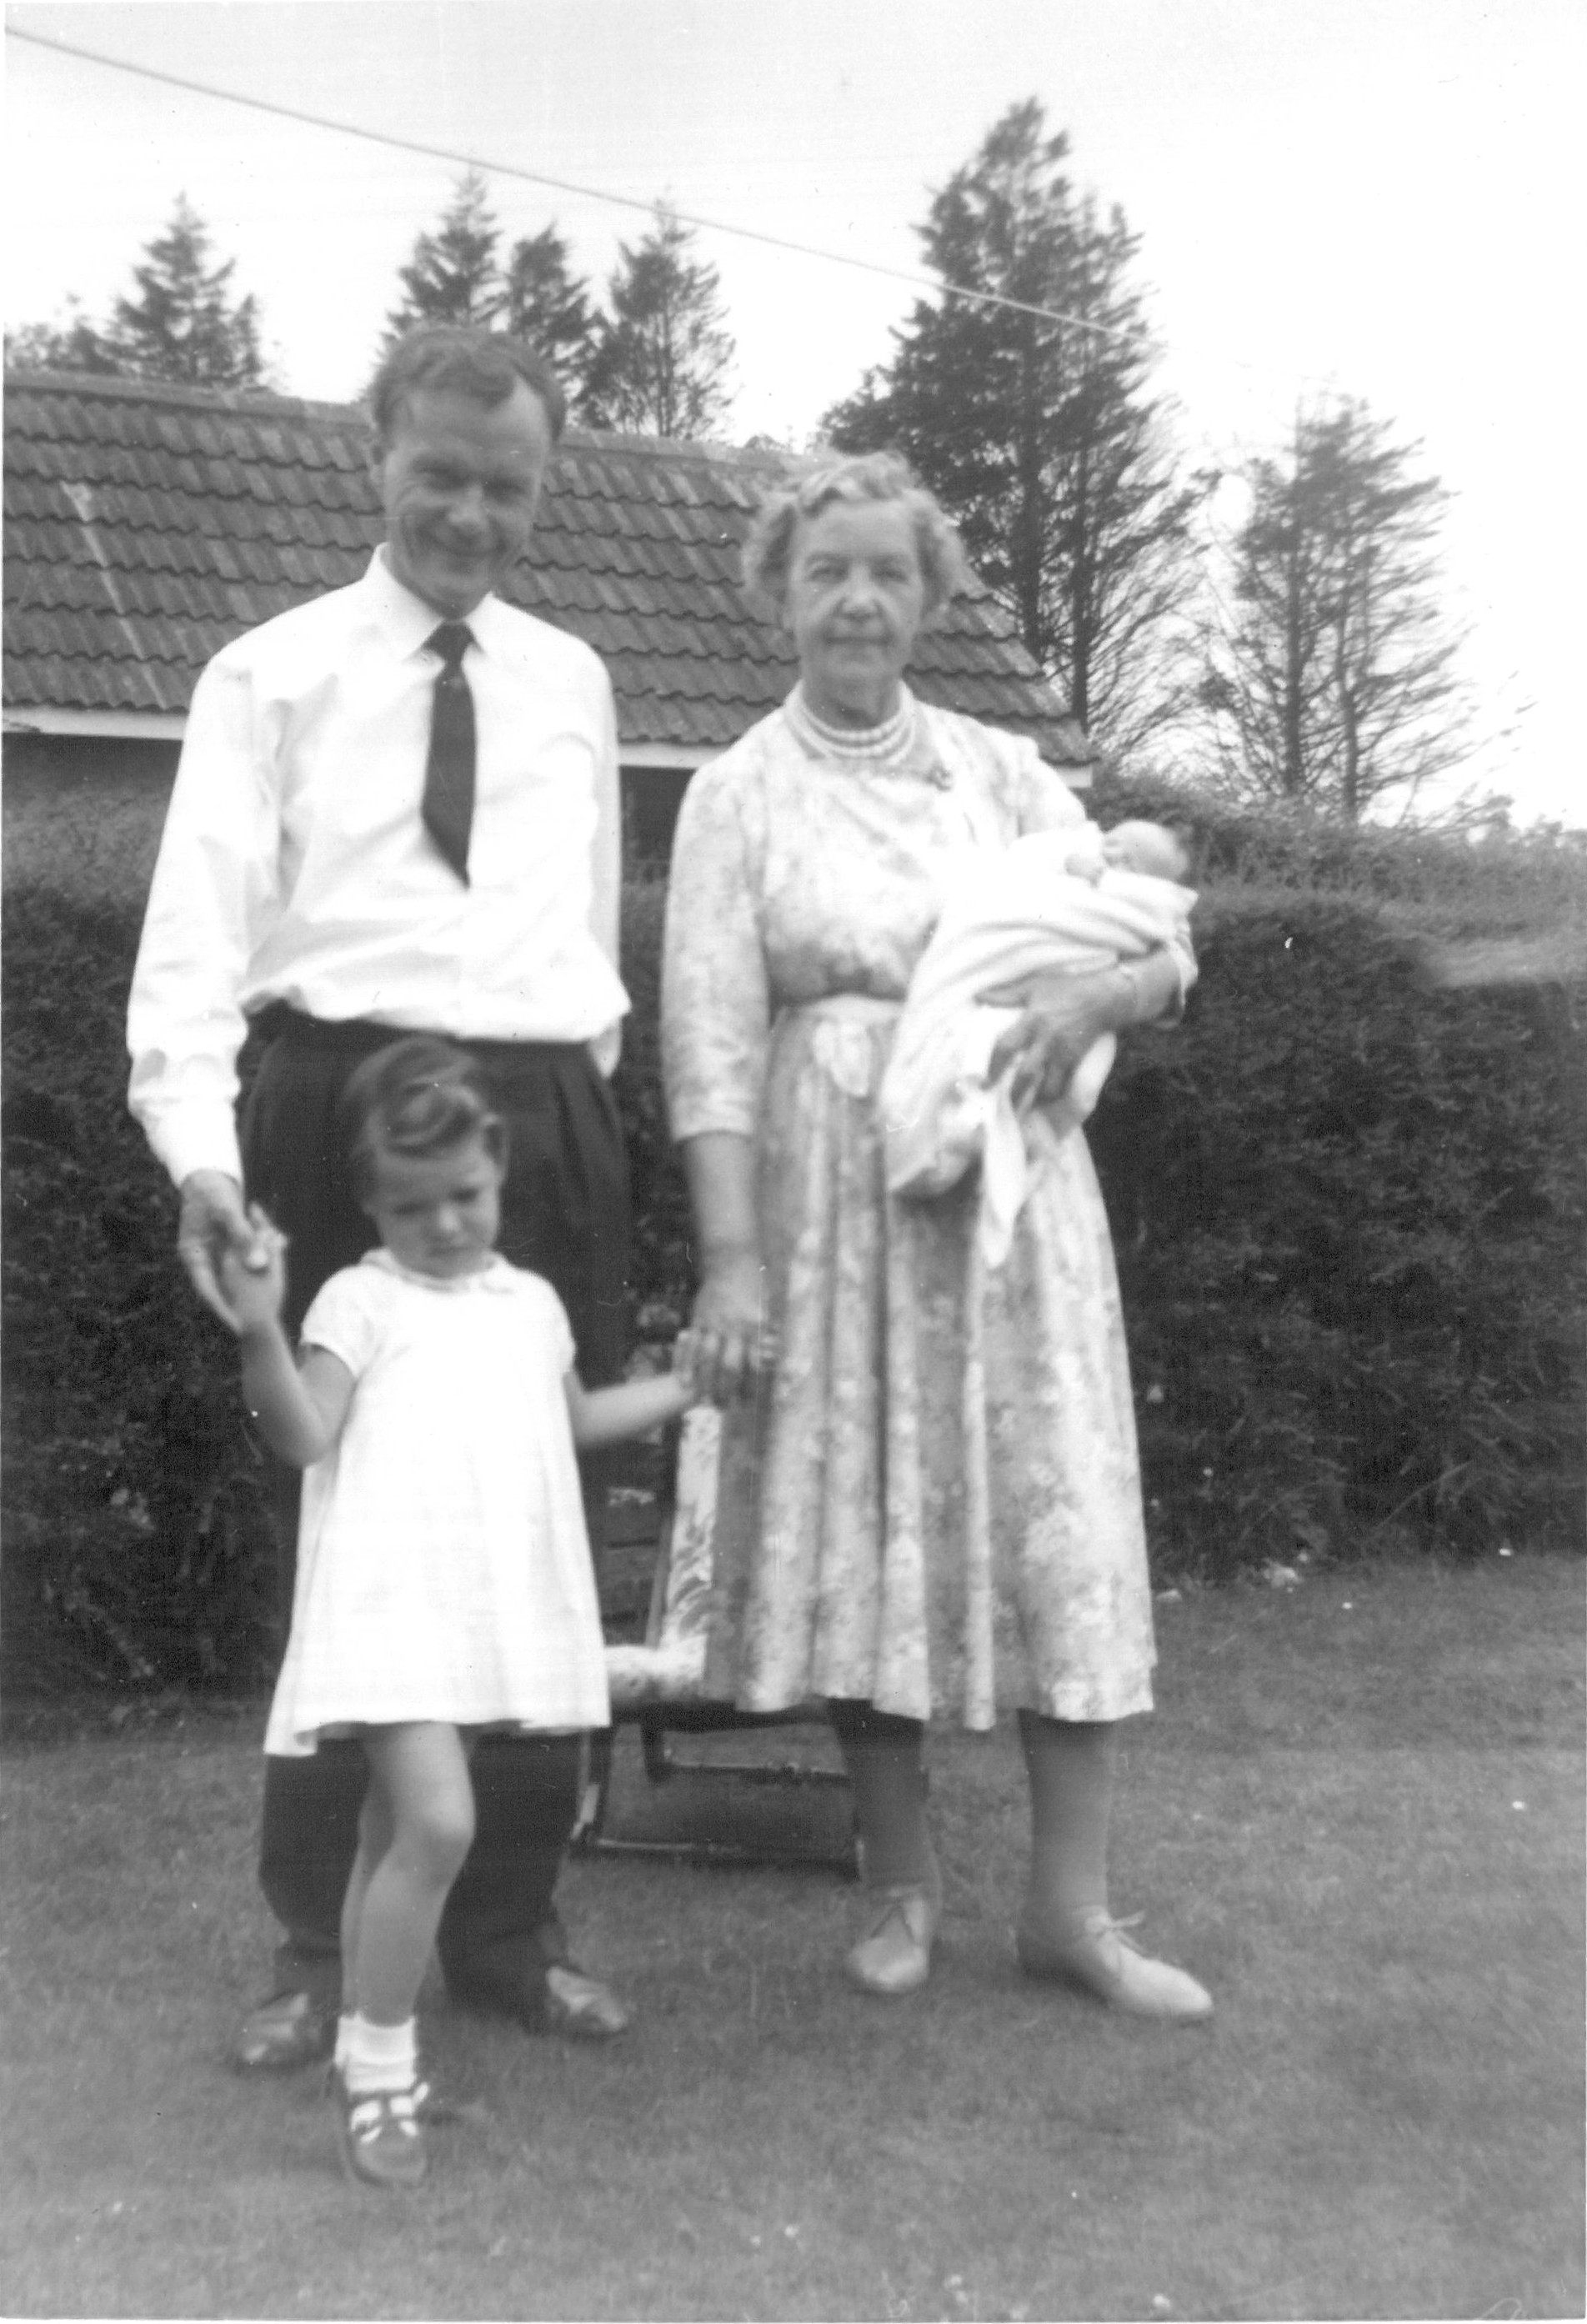
\includegraphics[width=0.45\textwidth]{photos/tony-with-mother.jpg}\label{tony-with-mother}}
    \\
  \end{tabular}
  \caption{Family (England, 1964).}
  \label{tony-family}
\end{figure}


Elizabeth became the ``Little mother.'' We had some laughs; a changed
nappy would finish up round his ankles and the lime juice once given
to him caused him serious problems.

When Richard was 4, he started going to St. Saviour's school and was
lucky to have Elizabeth there to keep an eye on him. He and Elizabeth
both enjoyed the school which was a very happy place (see
Picture~\ref{young-children}).

% \begin{figure}
%   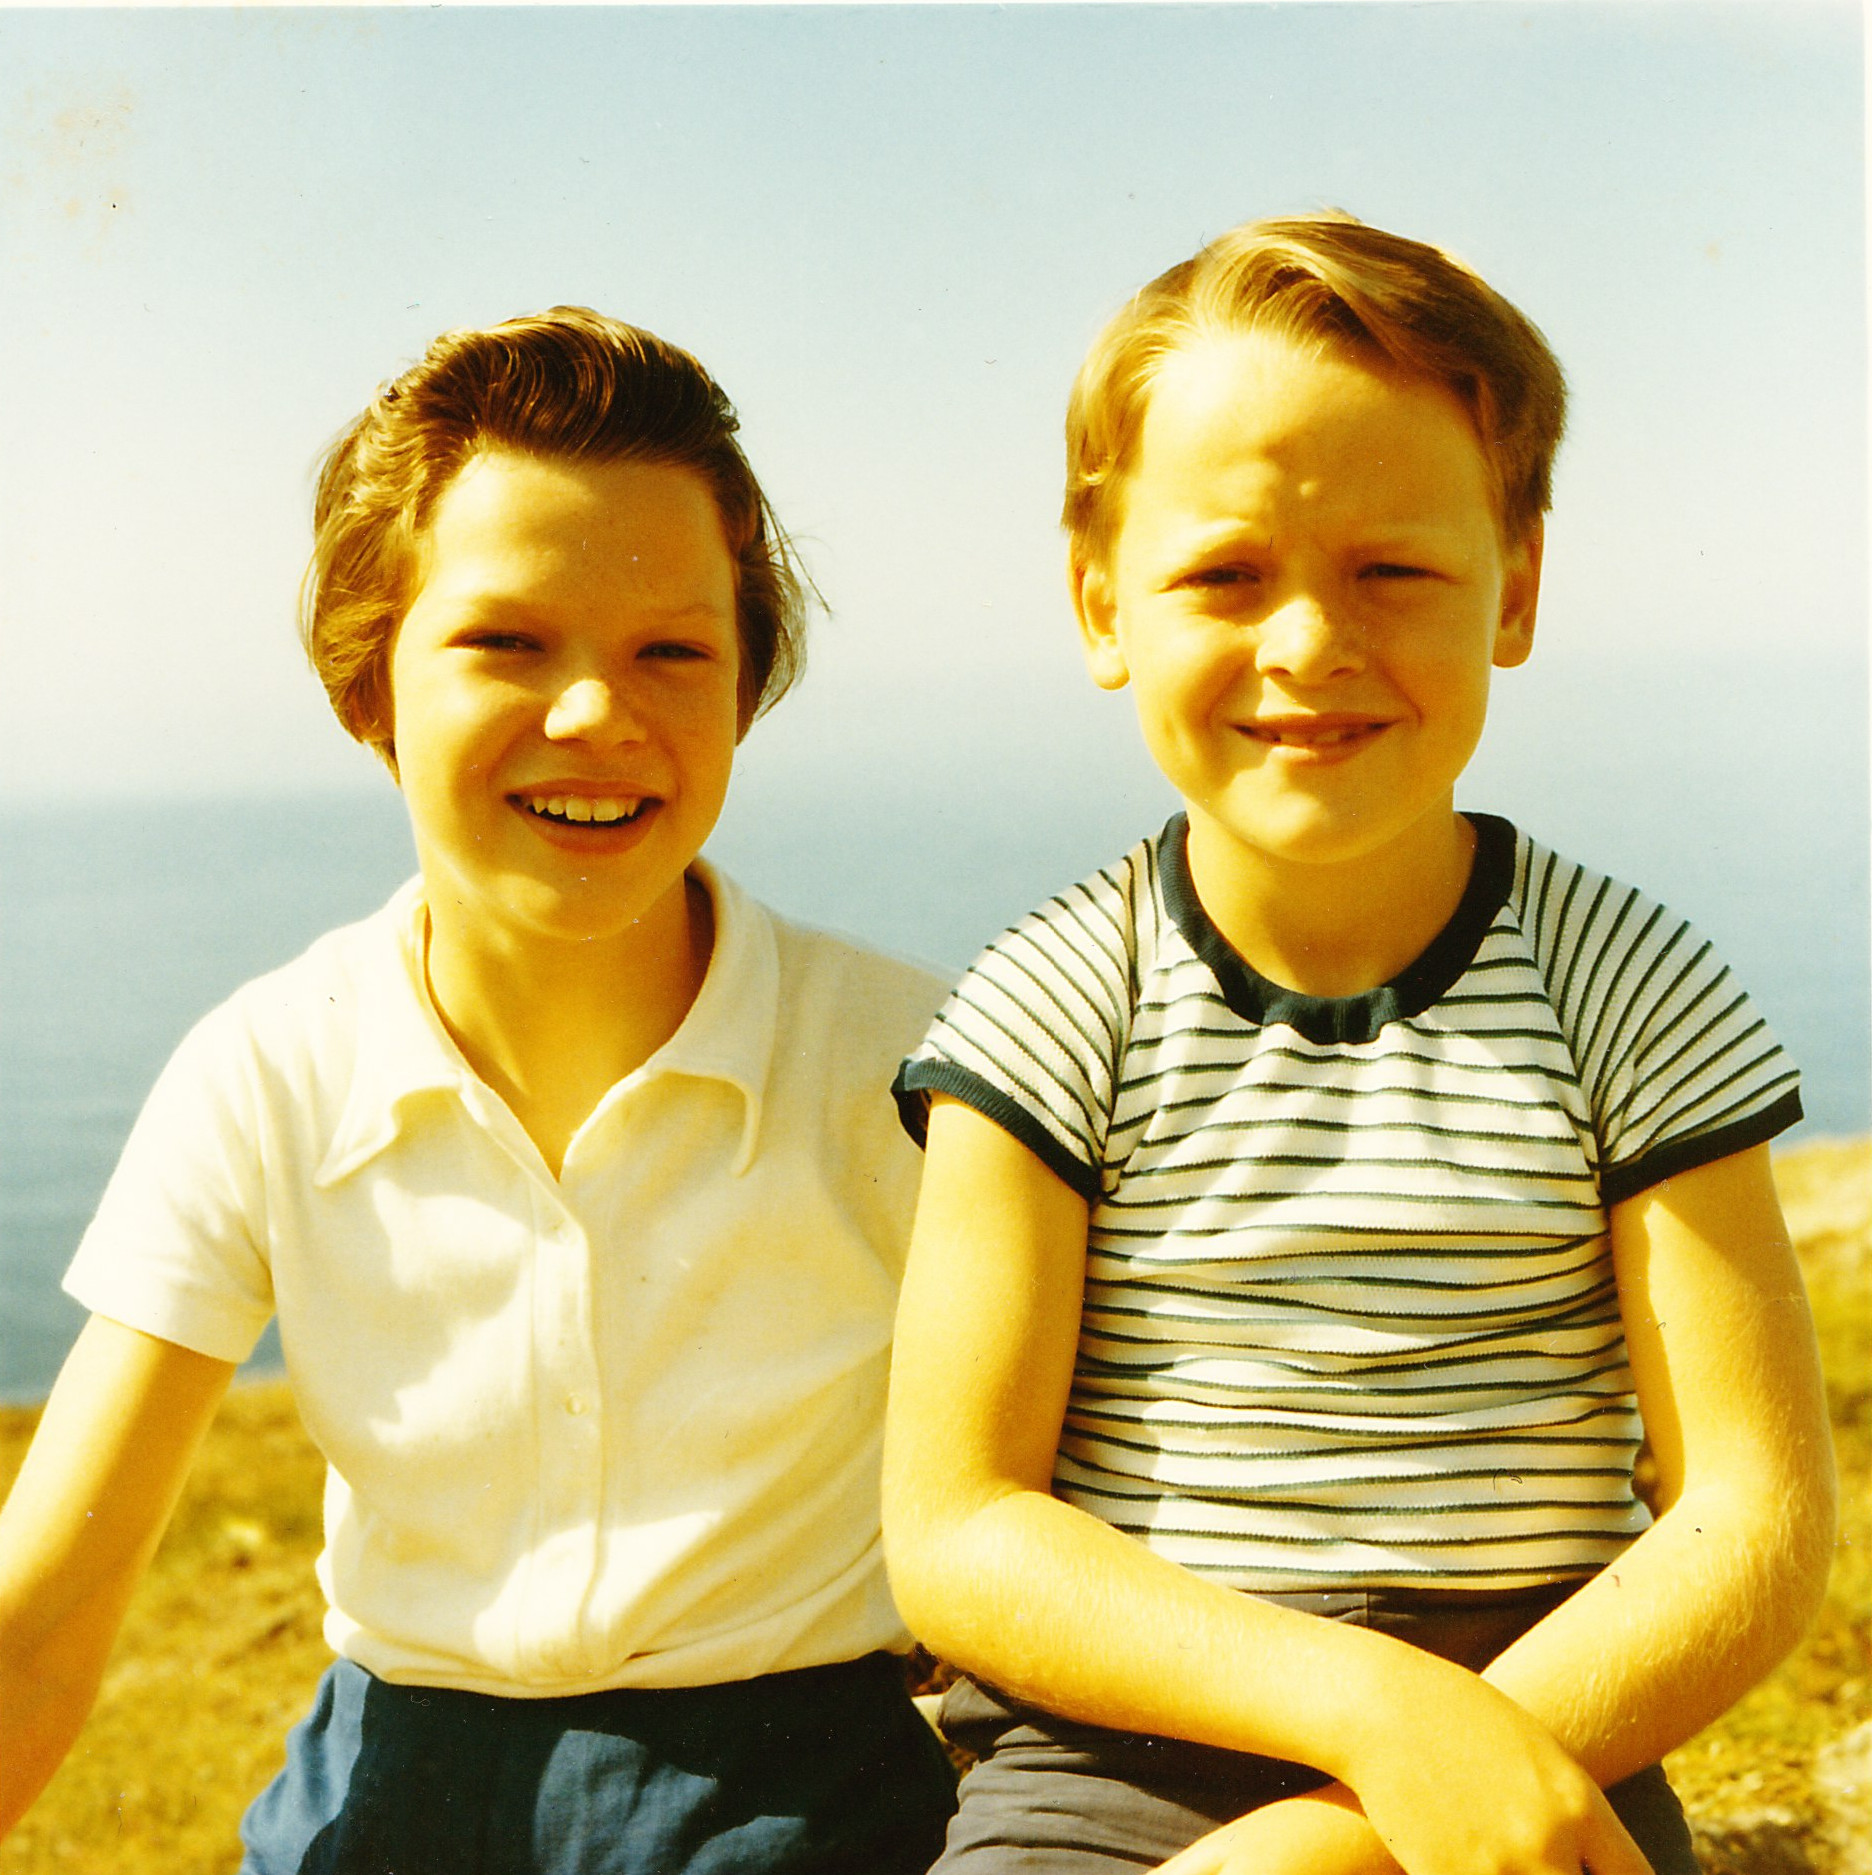
\includegraphics[width=\textwidth]{photos/elizabeth-and-richard}
%   \caption{Elizabeth and Richard.}
%   \label{young-children}
% \end{figure}

We warded off the dreaded malaria by taking regular
medication. Cholera became endemic while we were there and we had to
be more particular than ever about filtering and boiling the water.

And we were especially careful about the various diseases caused by
the parasites entering the body. The children often went into the
garden dressed only in pants and a light shirt but \textit{always}
shoes and socks because some of these delightful creatures would enter
through the feet.

Life continued happily until Elizabeth was 11 when, because there was
no further schooling for ex-patriot whites, we had to send her to a
boarding school in England. We chose Wroxall Abbey in Warwickshire and
she was reasonably happy there. The company (GEC) paid her holiday
fares to see us and she became a calm and seasoned traveller.

Richard continued at St.~Saviour's until he was 7 and then we moved to
South Africa and we were all together again.

We settled in Johannesburg (see Picture~\ref{bray-family}).

\begin{figure}
  \centering
  \begin{tabular}{c}
    \subfloat[Elizabeth \& Richard (1969).]{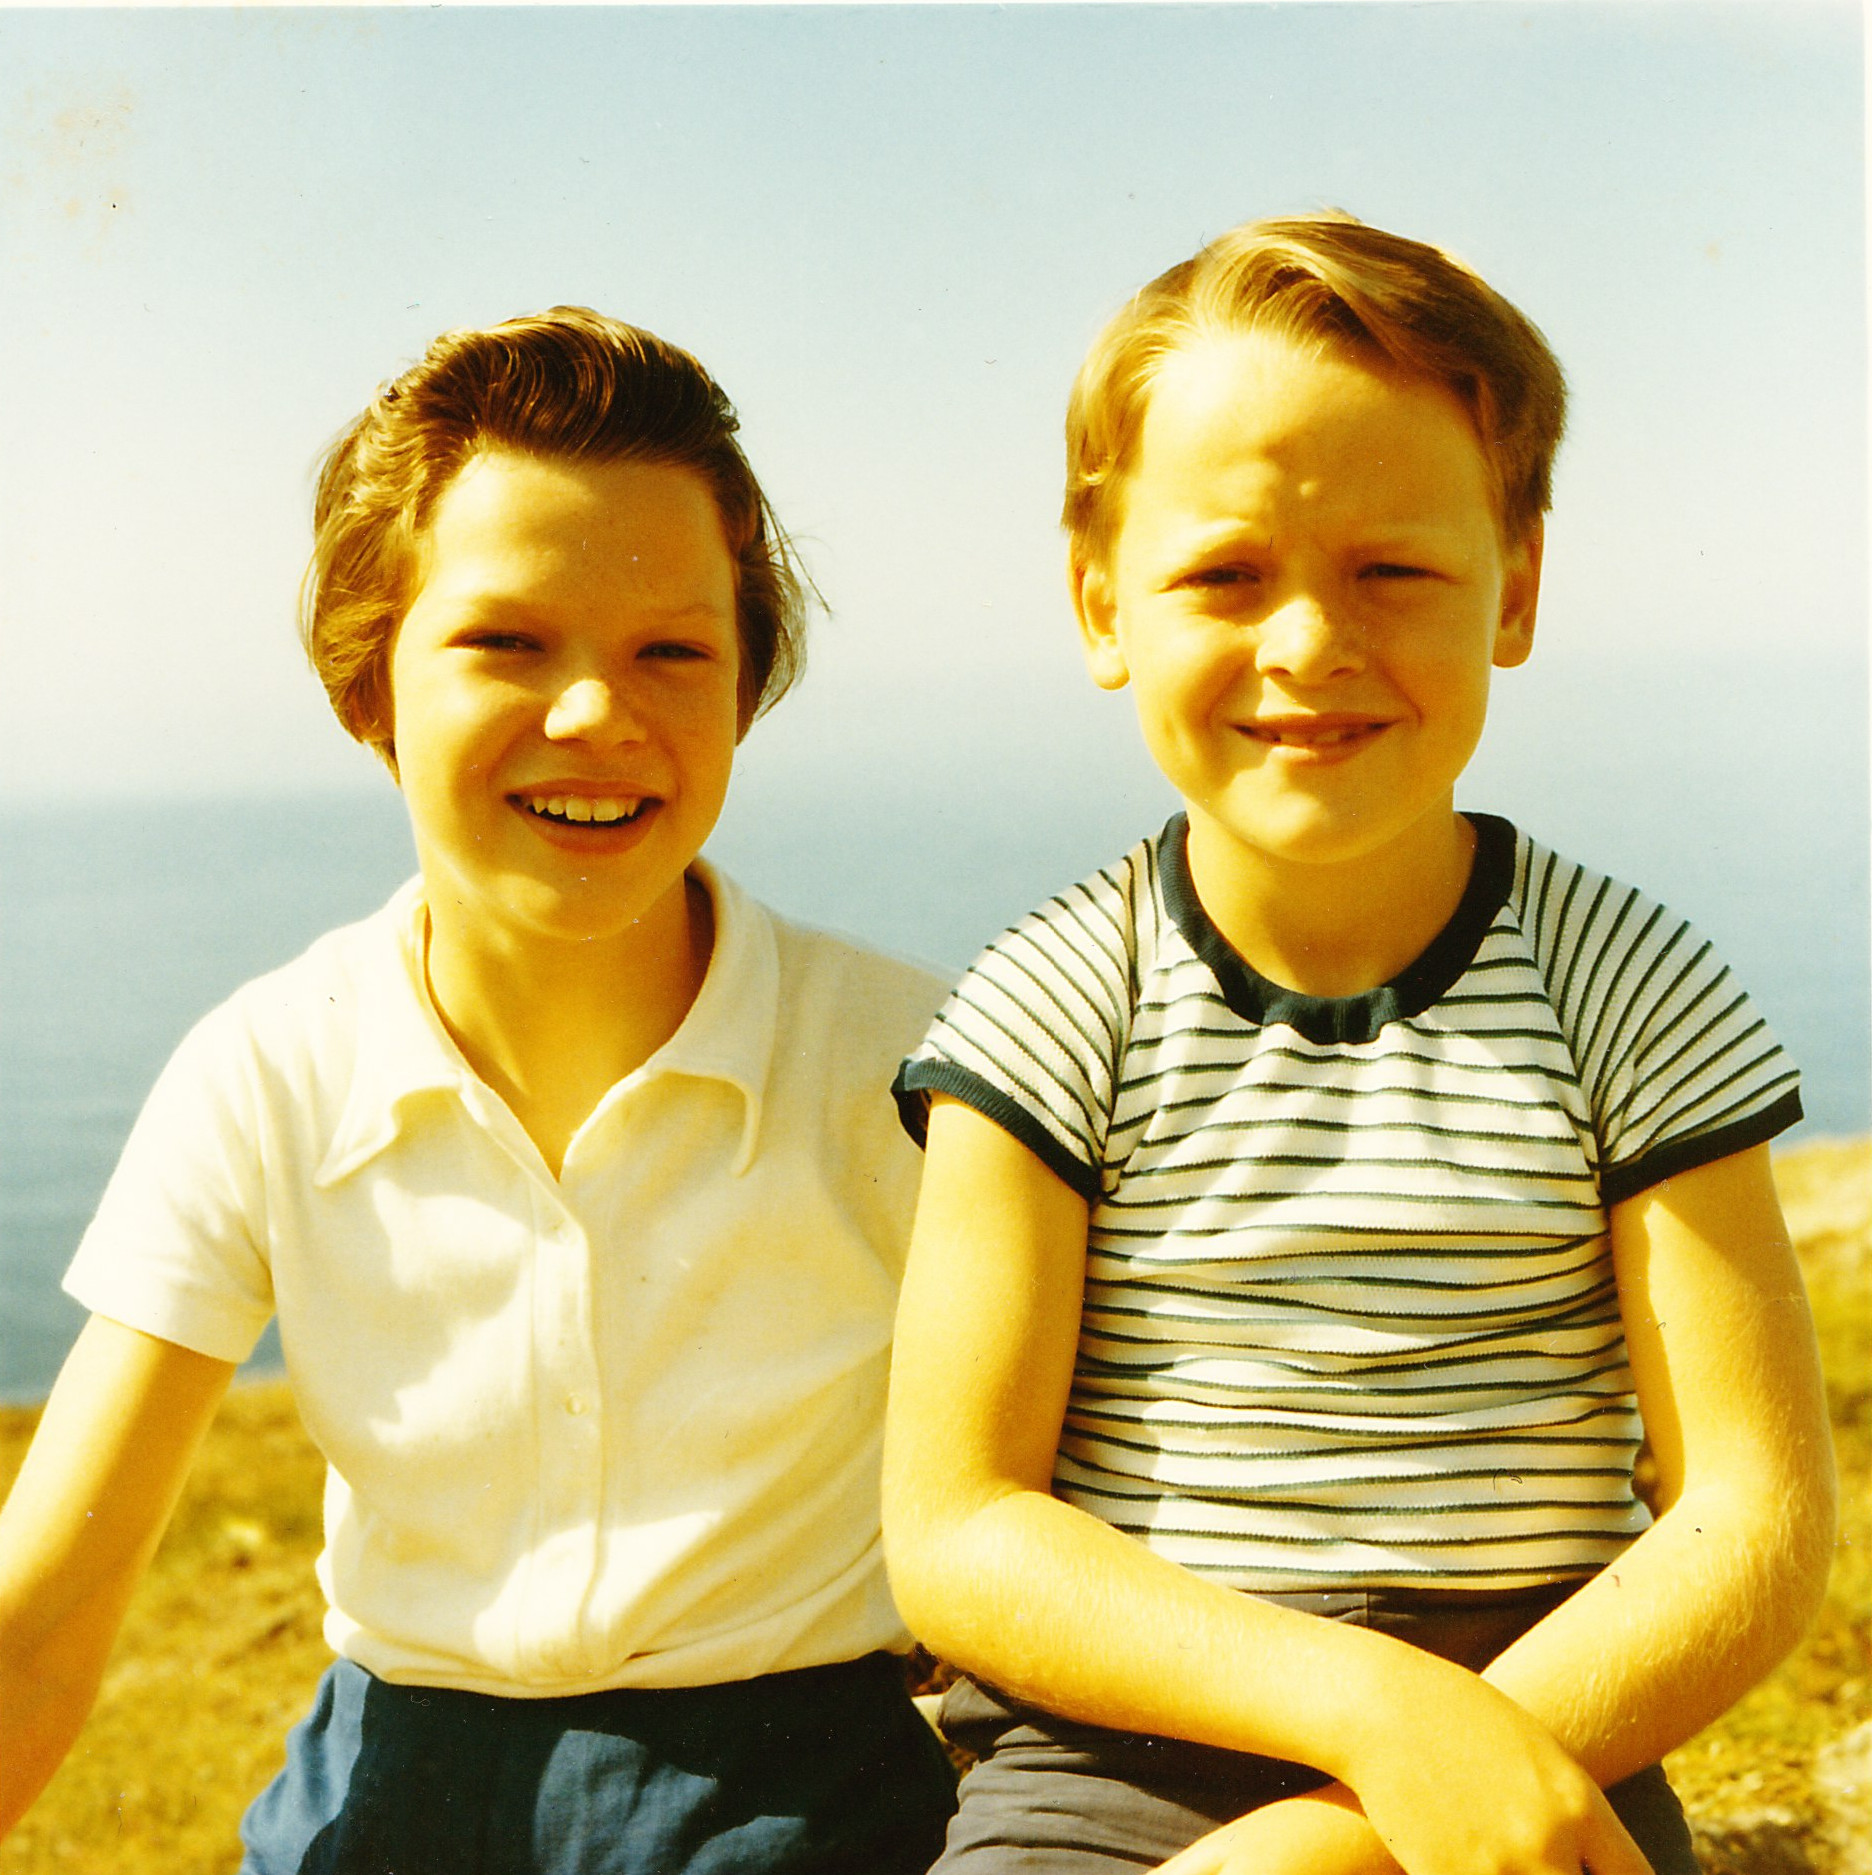
\includegraphics[width=0.6\textwidth]{photos/elizabeth-and-richard.jpg}\label{young-children}}
    \\
    \subfloat[Johannesburg (1975).]{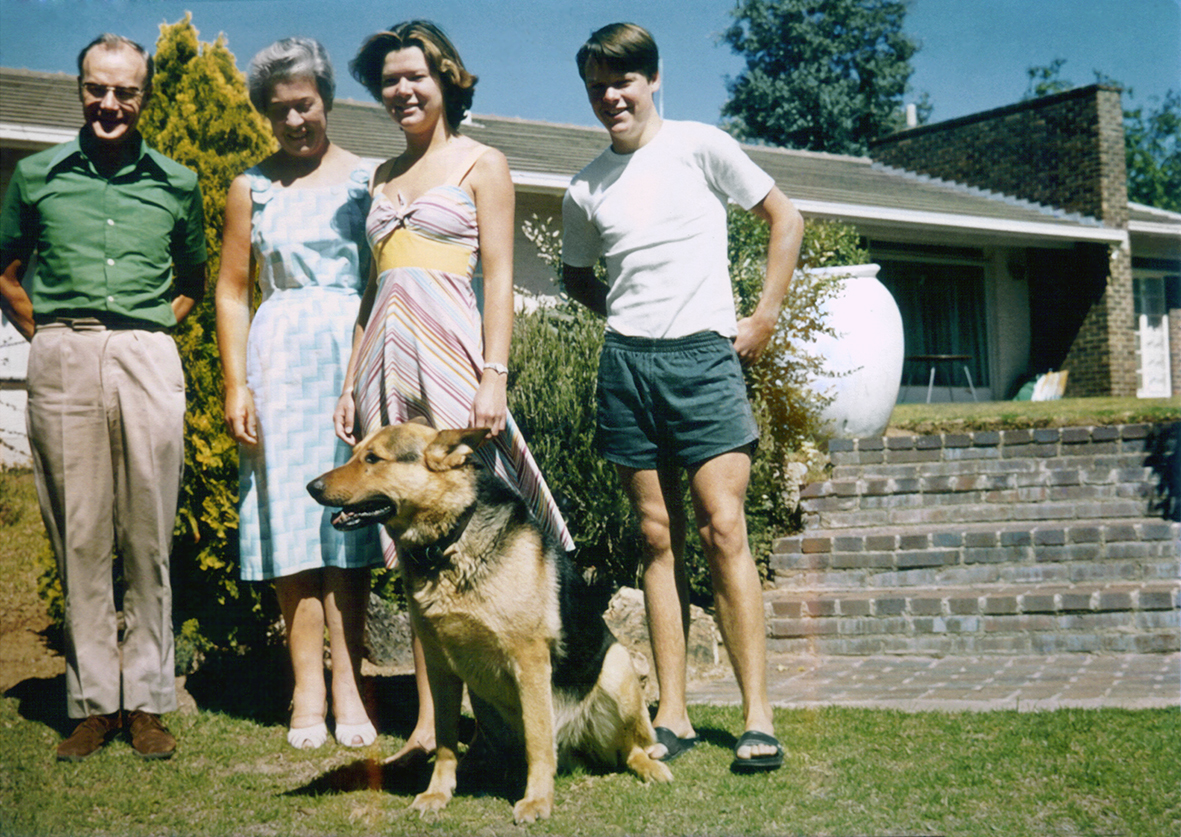
\includegraphics[width=0.8\textwidth]{photos/bray-family.jpg}\label{bray-family}}
    \\
  \end{tabular}
  \caption{Family years.}
  \label{family-years}
\end{figure}

% \begin{figure}
%   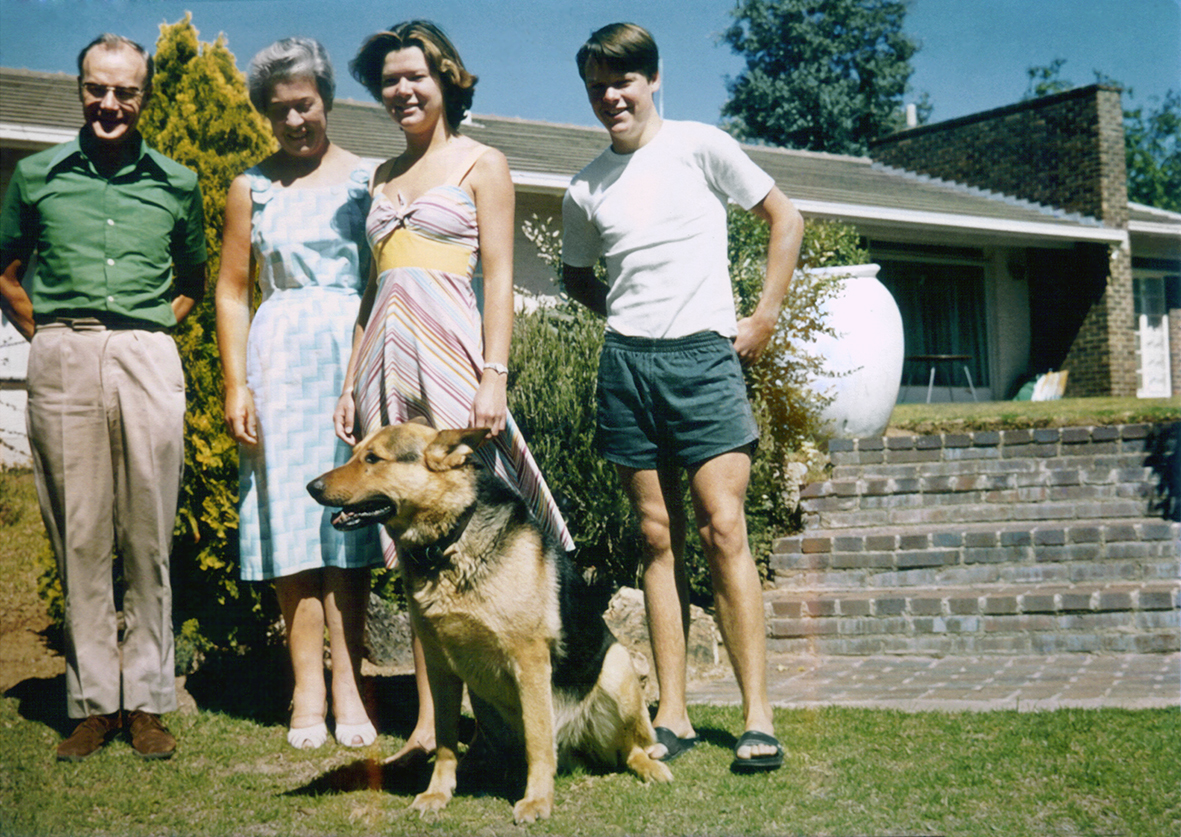
\includegraphics[width=\textwidth]{photos/bray-family}
%   \caption{The Bray family in Johannesburg.}
%   \label{bray-family}
% \end{figure}

Once more we had to look for schools and we chose Roedean\footnote{An
  offshoot of the Brighton school} for Elizabeth and St. John's for
Richard. Elizabeth was a day girl and I drove her to school and back
every day. The only way to apply for Richard to go to St. John's
college was to enroll him as a weekly boarder. He was only 8 (see
Picture~\ref{richard-school}).

% \begin{figure}
%   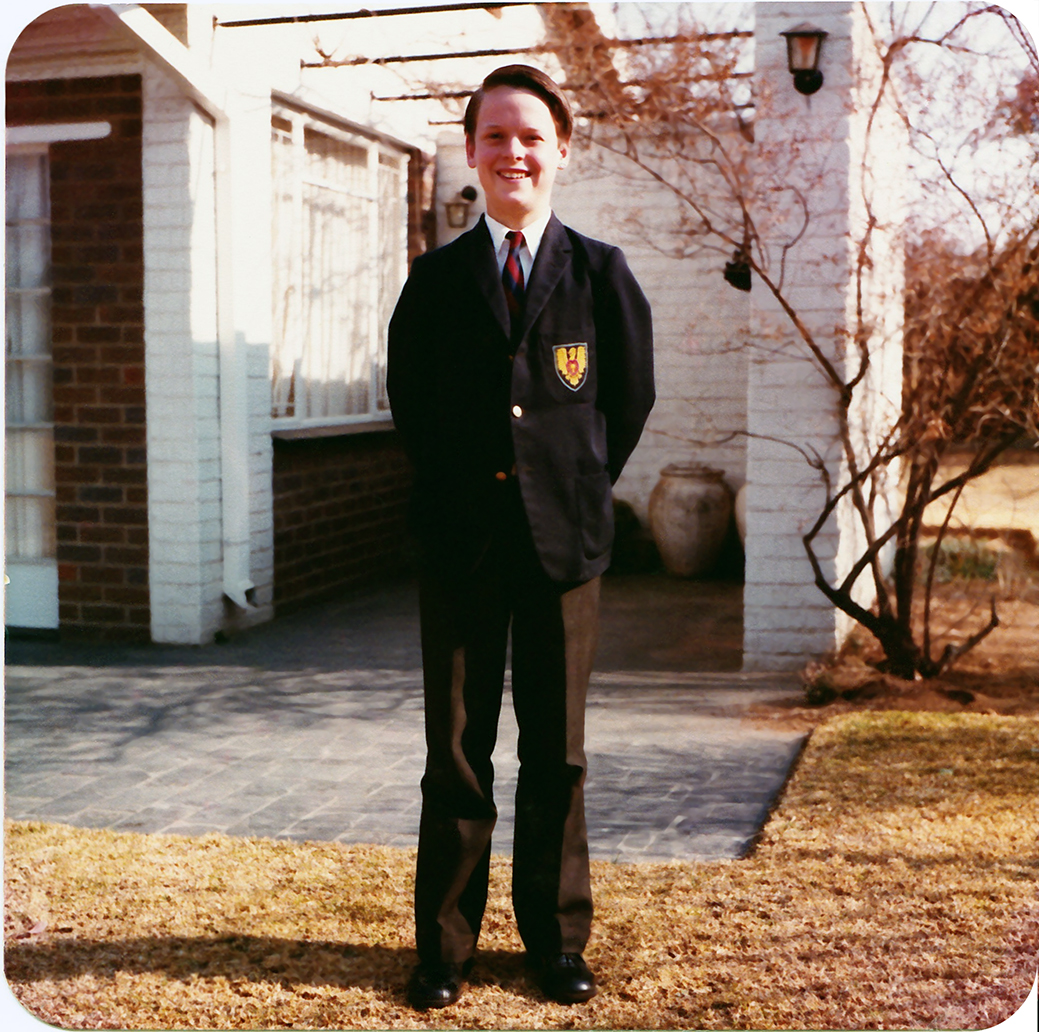
\includegraphics[width=\textwidth]{photos/richard-school}
%   \caption{Richard on his way to schoool.}
%   \label{richard-school}
% \end{figure}

Richard's love of cricket followed him through the school and he was
always chosen for the A-team as he moved up through the age groups. He
was a medium-pace bowler -- and very accurate -- and was awarded 2
hat-tricks during his career. We were very proud when he gained his
cricket colours in 1978.

Richard had decided on a hotel career and having gained his Matric, he
went immediately into hotel training. Starting off with Holiday Inn,
his first place was Secunda where he met his first wife and they were
to have 2 children. Unfortunately the marriage failed; they were both
too young and Richard needed time to develop his career. A junior
trainee is very much looked down upon but he stood his ground and had
gradual promotions to other Holiday Inn hotels, becoming more
confident and assured. Tony and I visited him in every one of the
hotels he worked in and, of course, this allowed us to see many parts
of the country. He progressed to Sun International and The
Sheraton. He met Pat, who was to become his second wife, and they
settled eventually in Cape Town, which is now his headquarters for he
is now operations manager for the Premier Group. Pat already had a
son, Robin, and their son, Bradley, was born in 1997. Giving us 4
grandchildren but more to come!

Elizabeth did well all through Roedean and gained a good
Matric. Immediately she embarked on her nurses training by choosing to
study nursing and complete a BSc. degree -- studying for long hours
and nursing at the Johannesburg hospital. This was a gruelling
4~years (see Picture~\ref{elizabeth-nurse}).

\begin{figure}
  \centering
  \begin{tabular}{cc}
    \subfloat{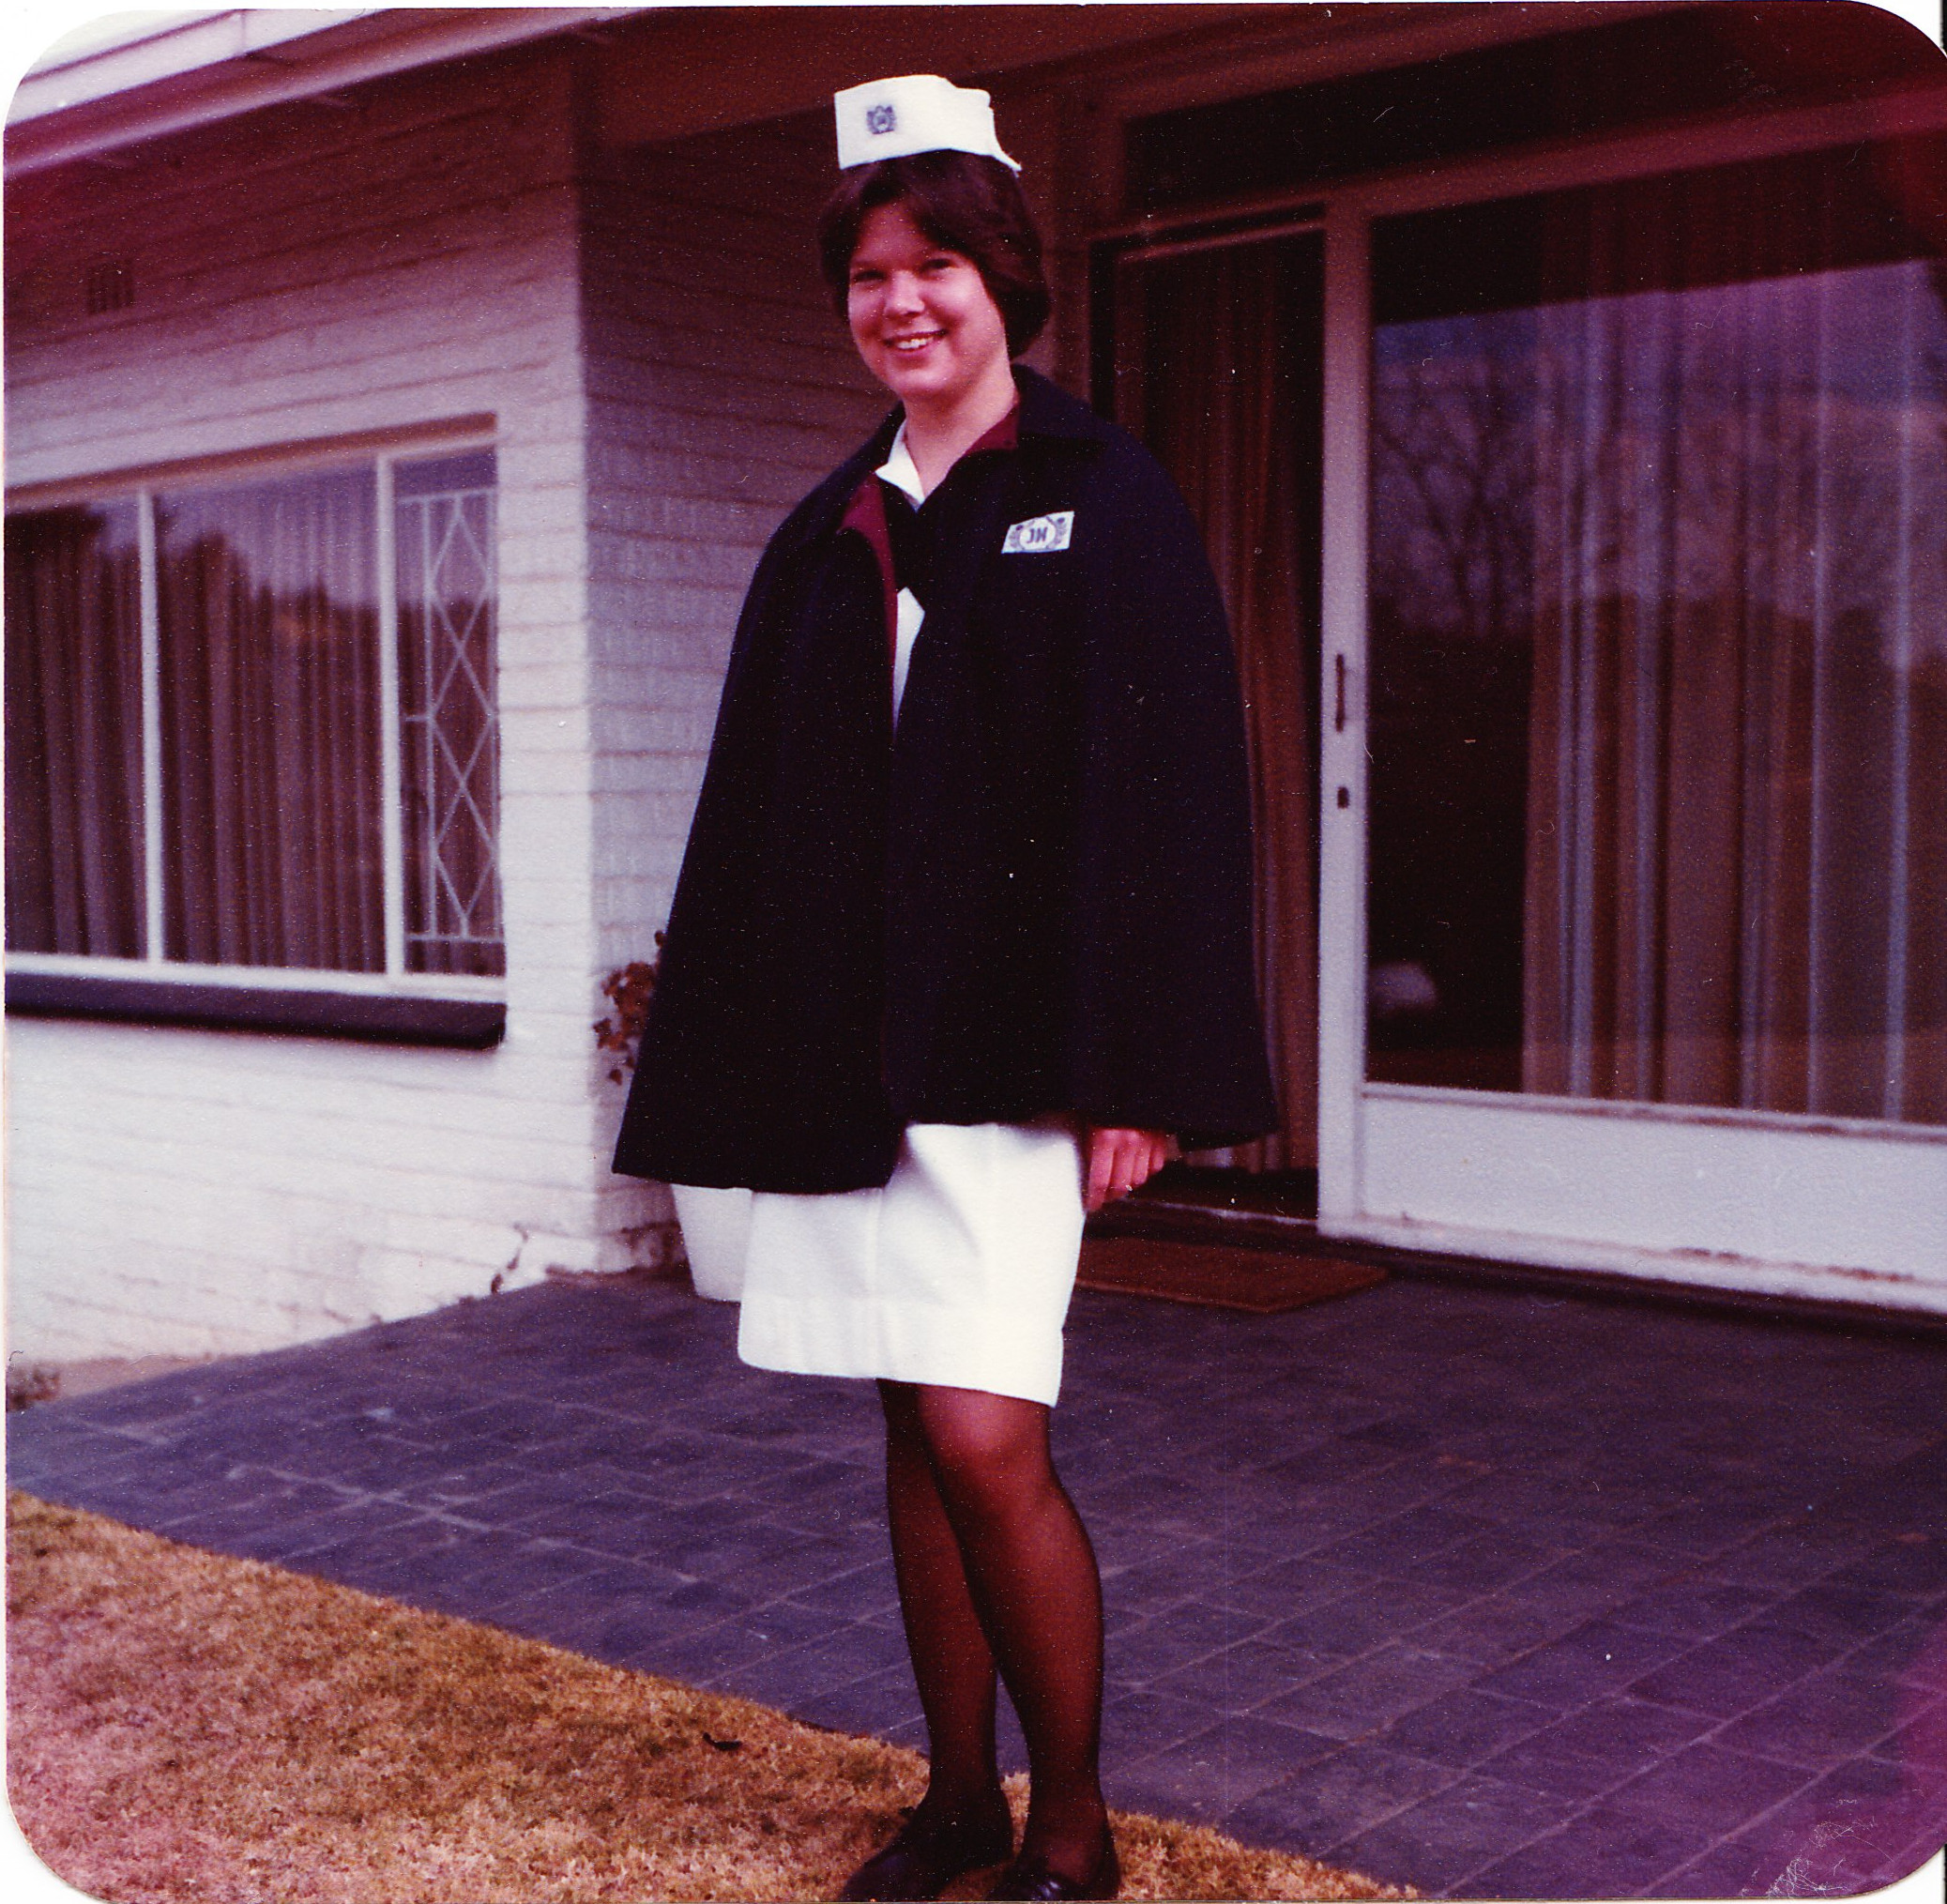
\includegraphics[width=0.45\textwidth]{photos/elizabeth-nurse.jpg}\label{elizabeth-nurse}}
    &
    \subfloat{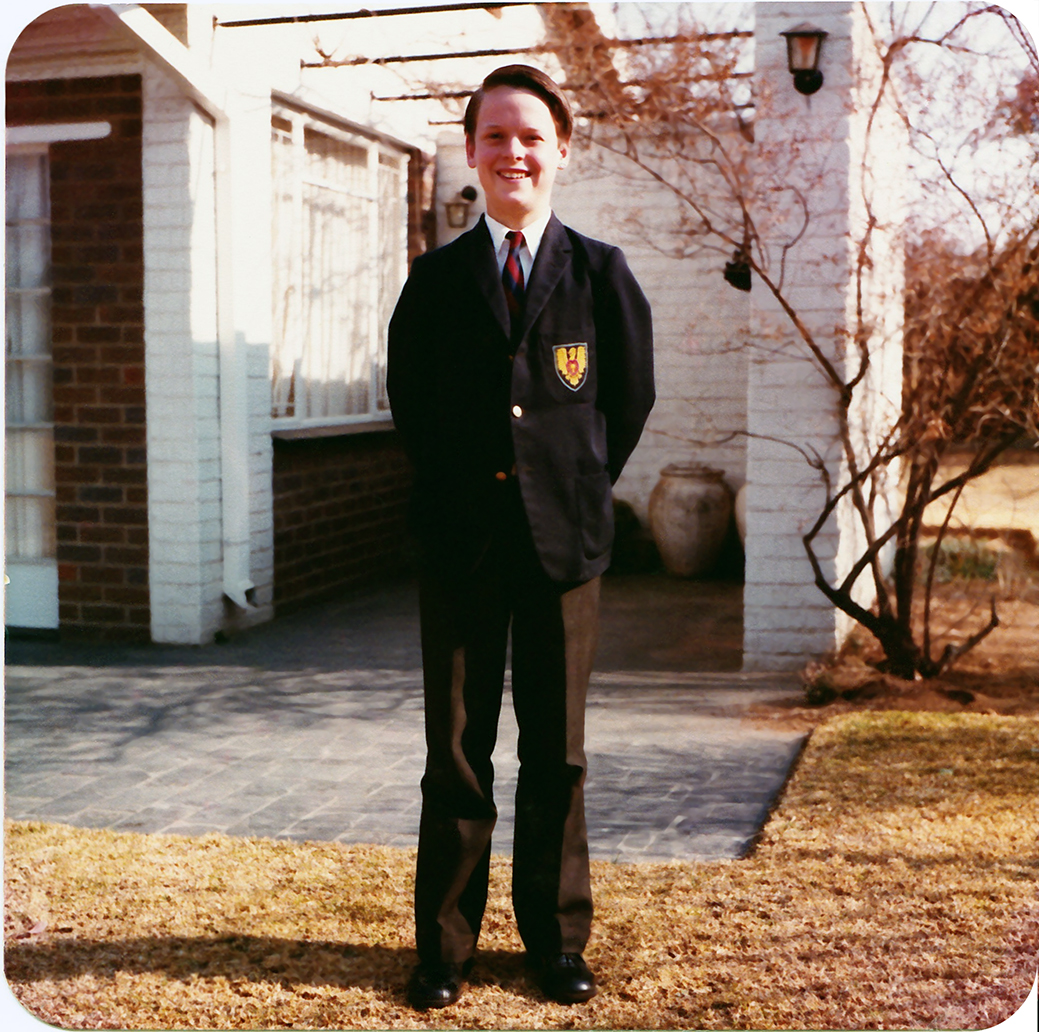
\includegraphics[width=0.45\textwidth]{photos/richard-school.jpg}\label{richard-school}}
    \\
  \end{tabular}
  \caption{Elizabeth (aged 18) \& Richard (aged 16).}
  \label{children}
\end{figure}

% \begin{figure}
%   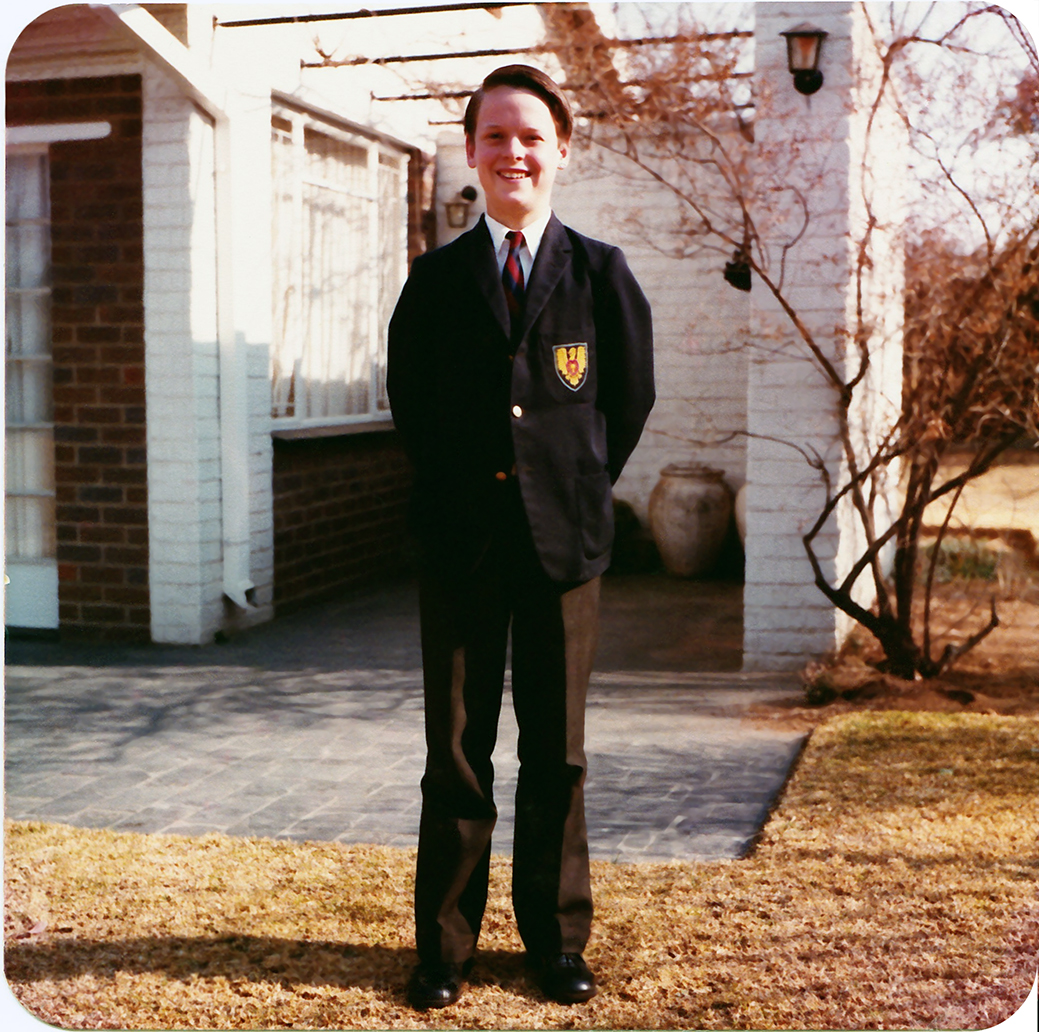
\includegraphics[width=\textwidth]{photos/richard-school}
%   \caption{Richard on his way to schoool.}
%   \label{richard-school}
% \end{figure}

% \begin{figure}
%   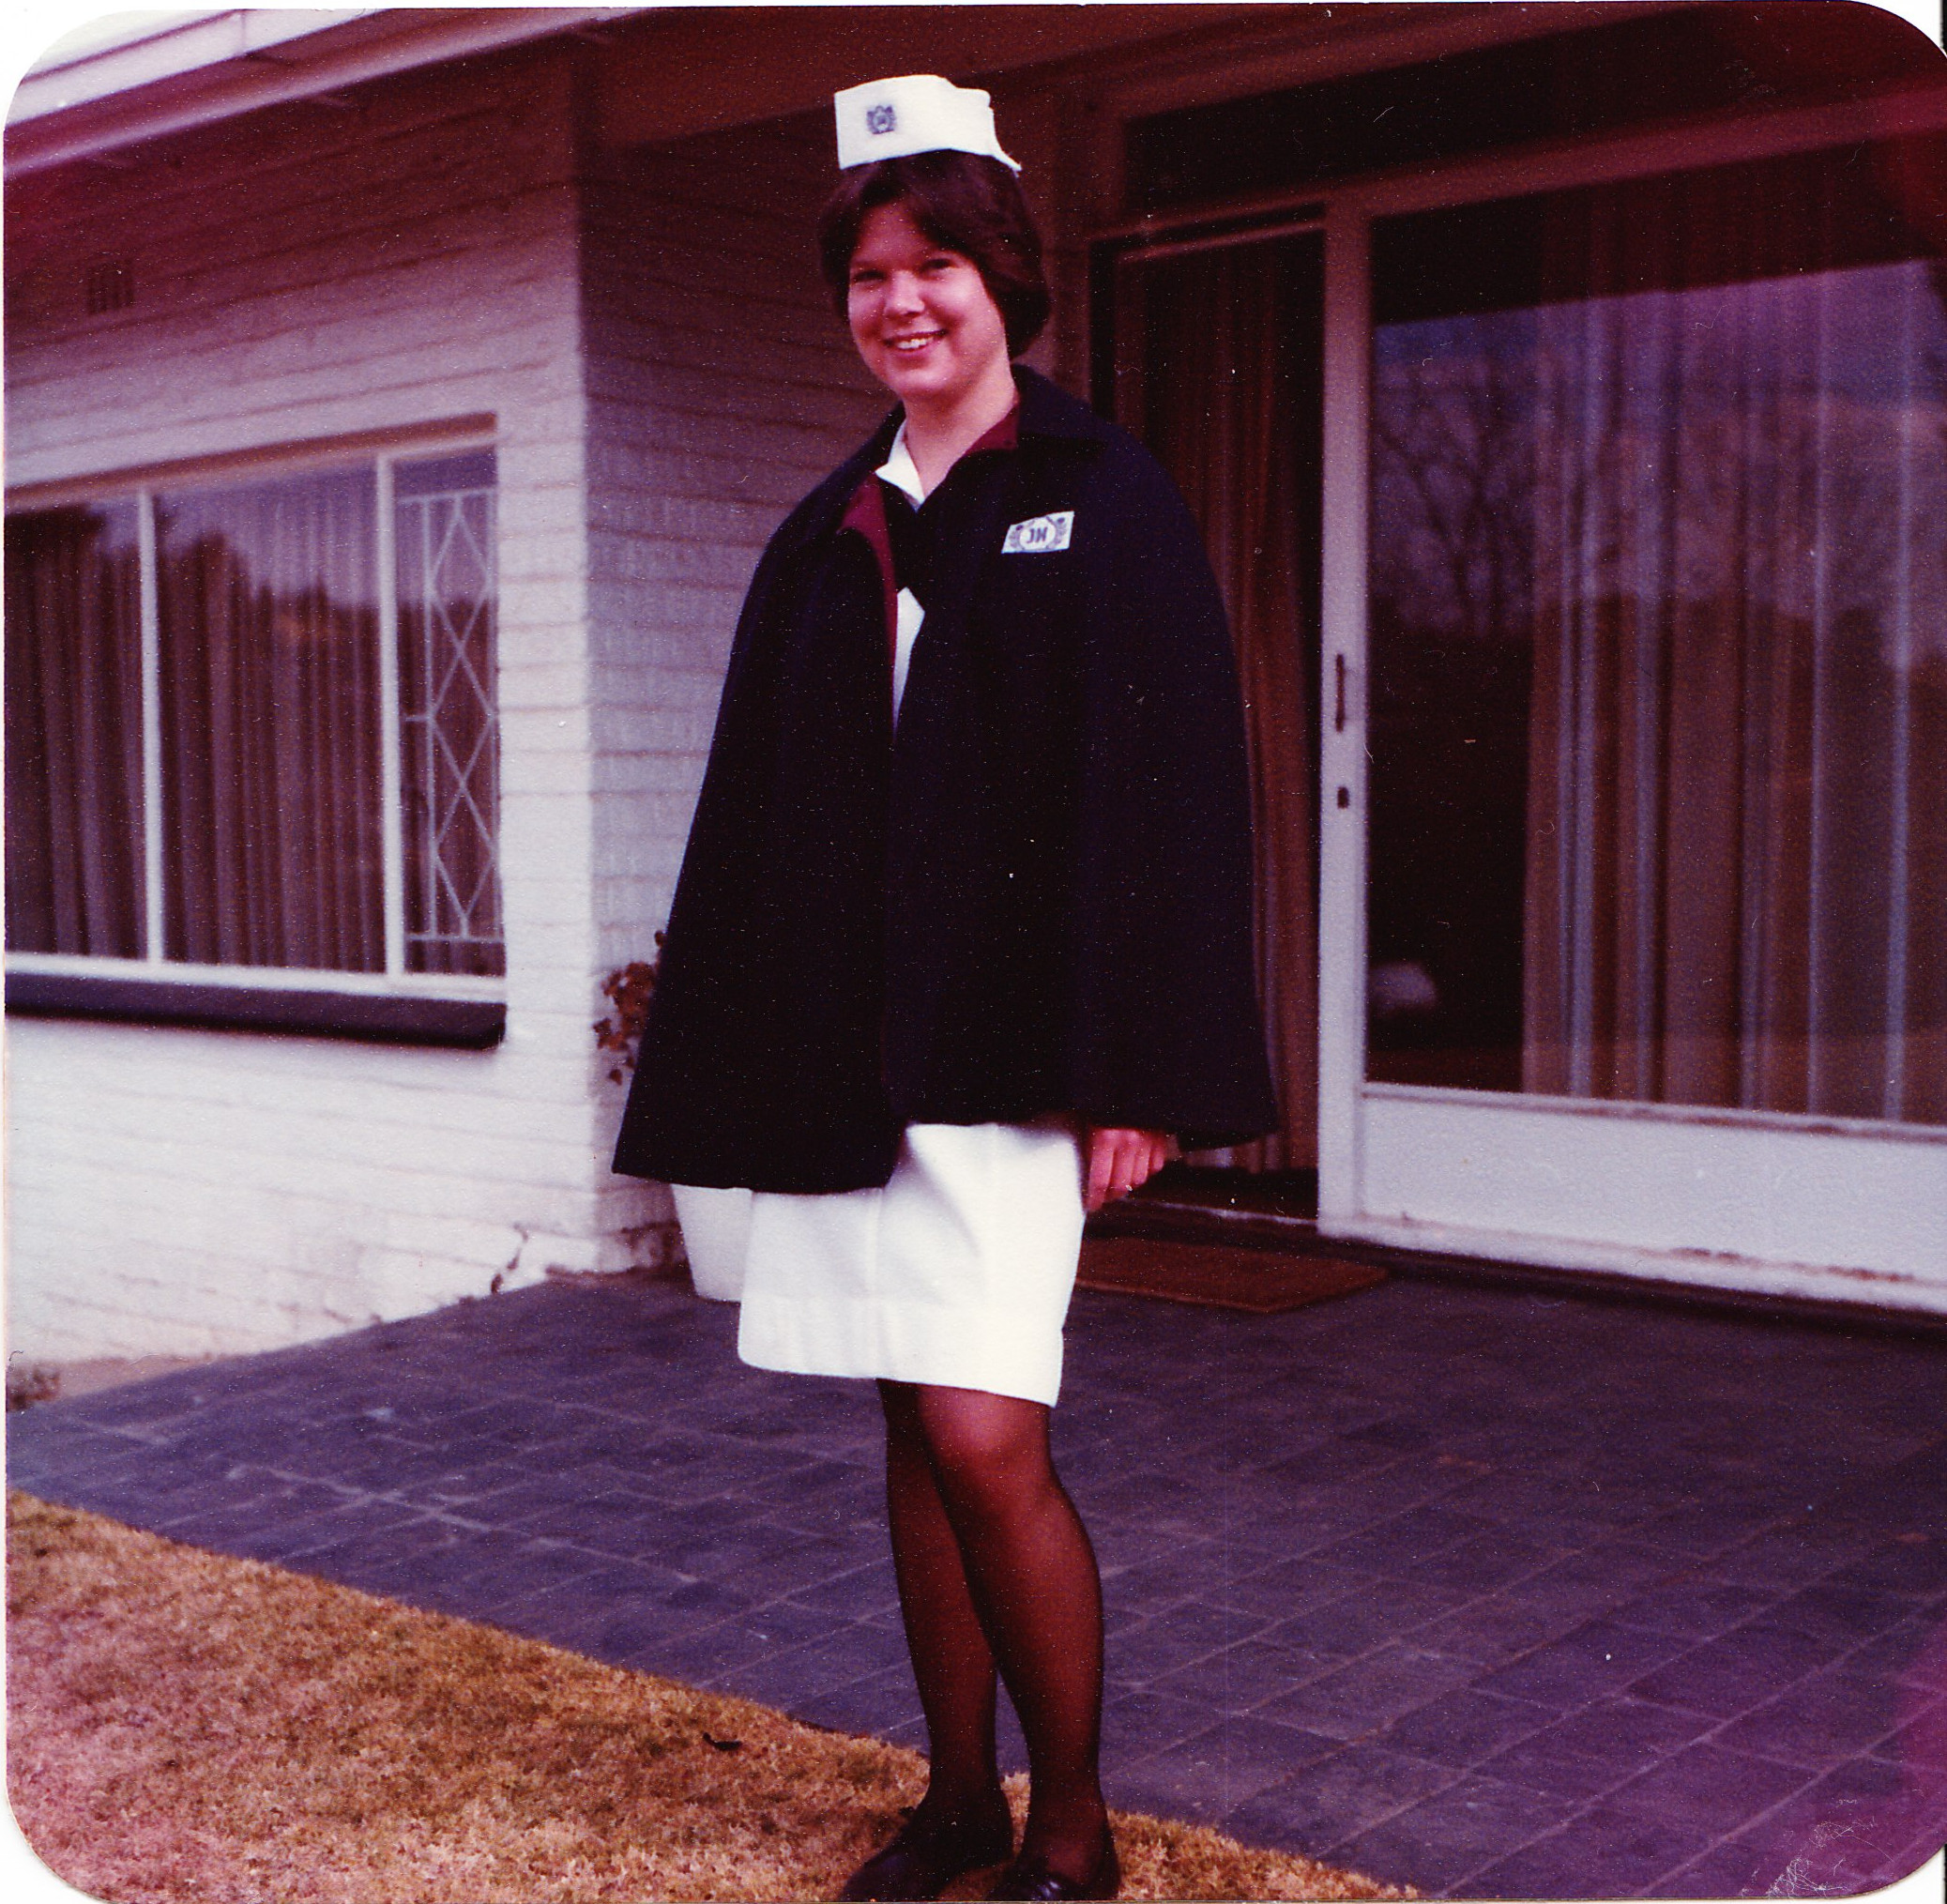
\includegraphics[width=\textwidth]{photos/elizabeth-nurse}
%   \caption{Elizabeth as a nurse.}
%   \label{elizabeth-nurse}
% \end{figure}

While training, she was knocked off a (borrowed) motorbike and had to
be hospitalized with a fractured femur. There she met, and was
attended to, by a young registrar, Matthew Preston, whom she would
eventually marry.

Once she came home from the hospital there was work to be done on the
injured leg. The effort of bending the leg at the knee was terribly
painful and I had to help her with the exercises. I don't know who
suffered the most -- the pain to her was hideous, but she persevered.

Because of her hospitalization, Elizabeth was not able to write her
final exam with the other students. She was permitted to do this later
in a private room.

This was on her 21st birthday and on that very day -- July 21st, 1981
-- Prince Charles and Princess Diana were married. She never did get
to see a video of the wedding! However she succeeded in passing her
final exam. And we were all overjoyed.

Elizabeth and Matthew were married in August 1982 and the wedding took
place in the Roedean chapel; the reception was held at the Wanderers
Club, Johannesburg. It was a very happy occasion but, sadly the
marriage failed after 23~years. During that time 4 wonderful children
were born -- Andrew, Claire, Lisa, and Shaun.

Tony and I suffered a lot of heartache over our childrens' divorces,
but were happy that they have both found happiness. In New Zealand,
Elizabeth was brave enough to resume her studies in nursing and gained
her masters degree in 2012.

It was sad that Tony had to miss this wonderful achievement. He would
have been proud; I found enough pride for both of us. Meanwhile,
Elizabeth continues with her work in ICU.


\chapter{Grandchildren}

Andrew, Claire, Lisa, and Shaun.

Ryan, Kelly-Ann, Robin, and Bradley.

I am of the firm belief that children need their grandparents as much
as the oldies need the younger ones.

I value the friendship and support of my grandchildren very much and I
think mainly because I grew up in the era when the oldies were very
strict (and parents too) and affection did not come very much to the
fore. I love the more free and easy way of living today albeit gone a
little too far regarding discipline etc.

Frankly I dreaded my annual 2~weeks summer holiday with my mother's
mother. She never showed me much affection, dressed always in purple
or black and her hair was scraped into a topknot -- in other words she
was a very severe old lady; she was always old to me.

My other grandmother was vague and disinterested and my grandfather
was always pushing the bible, which did nothing to interest a young
girl.

How much more interest is shown in grandchildren today.

Many mothers go out to work and the oldies have the pleasure and
responsibility of looking after the children and this does form a
remarkable bond.

I have pleasant memories of babysitting with all of Elizabeth's
children.

Once, when Andrew and I were busy with lego, he put into play his
favourite word of the month which was ``obviously''. ``Obviously you
haven't read the instructions properly, Grandma.'' -- he was right --
I seldom read instructions properly (see Picture~\ref{madge-and-andrew}).

\begin{figure}
  \centering
  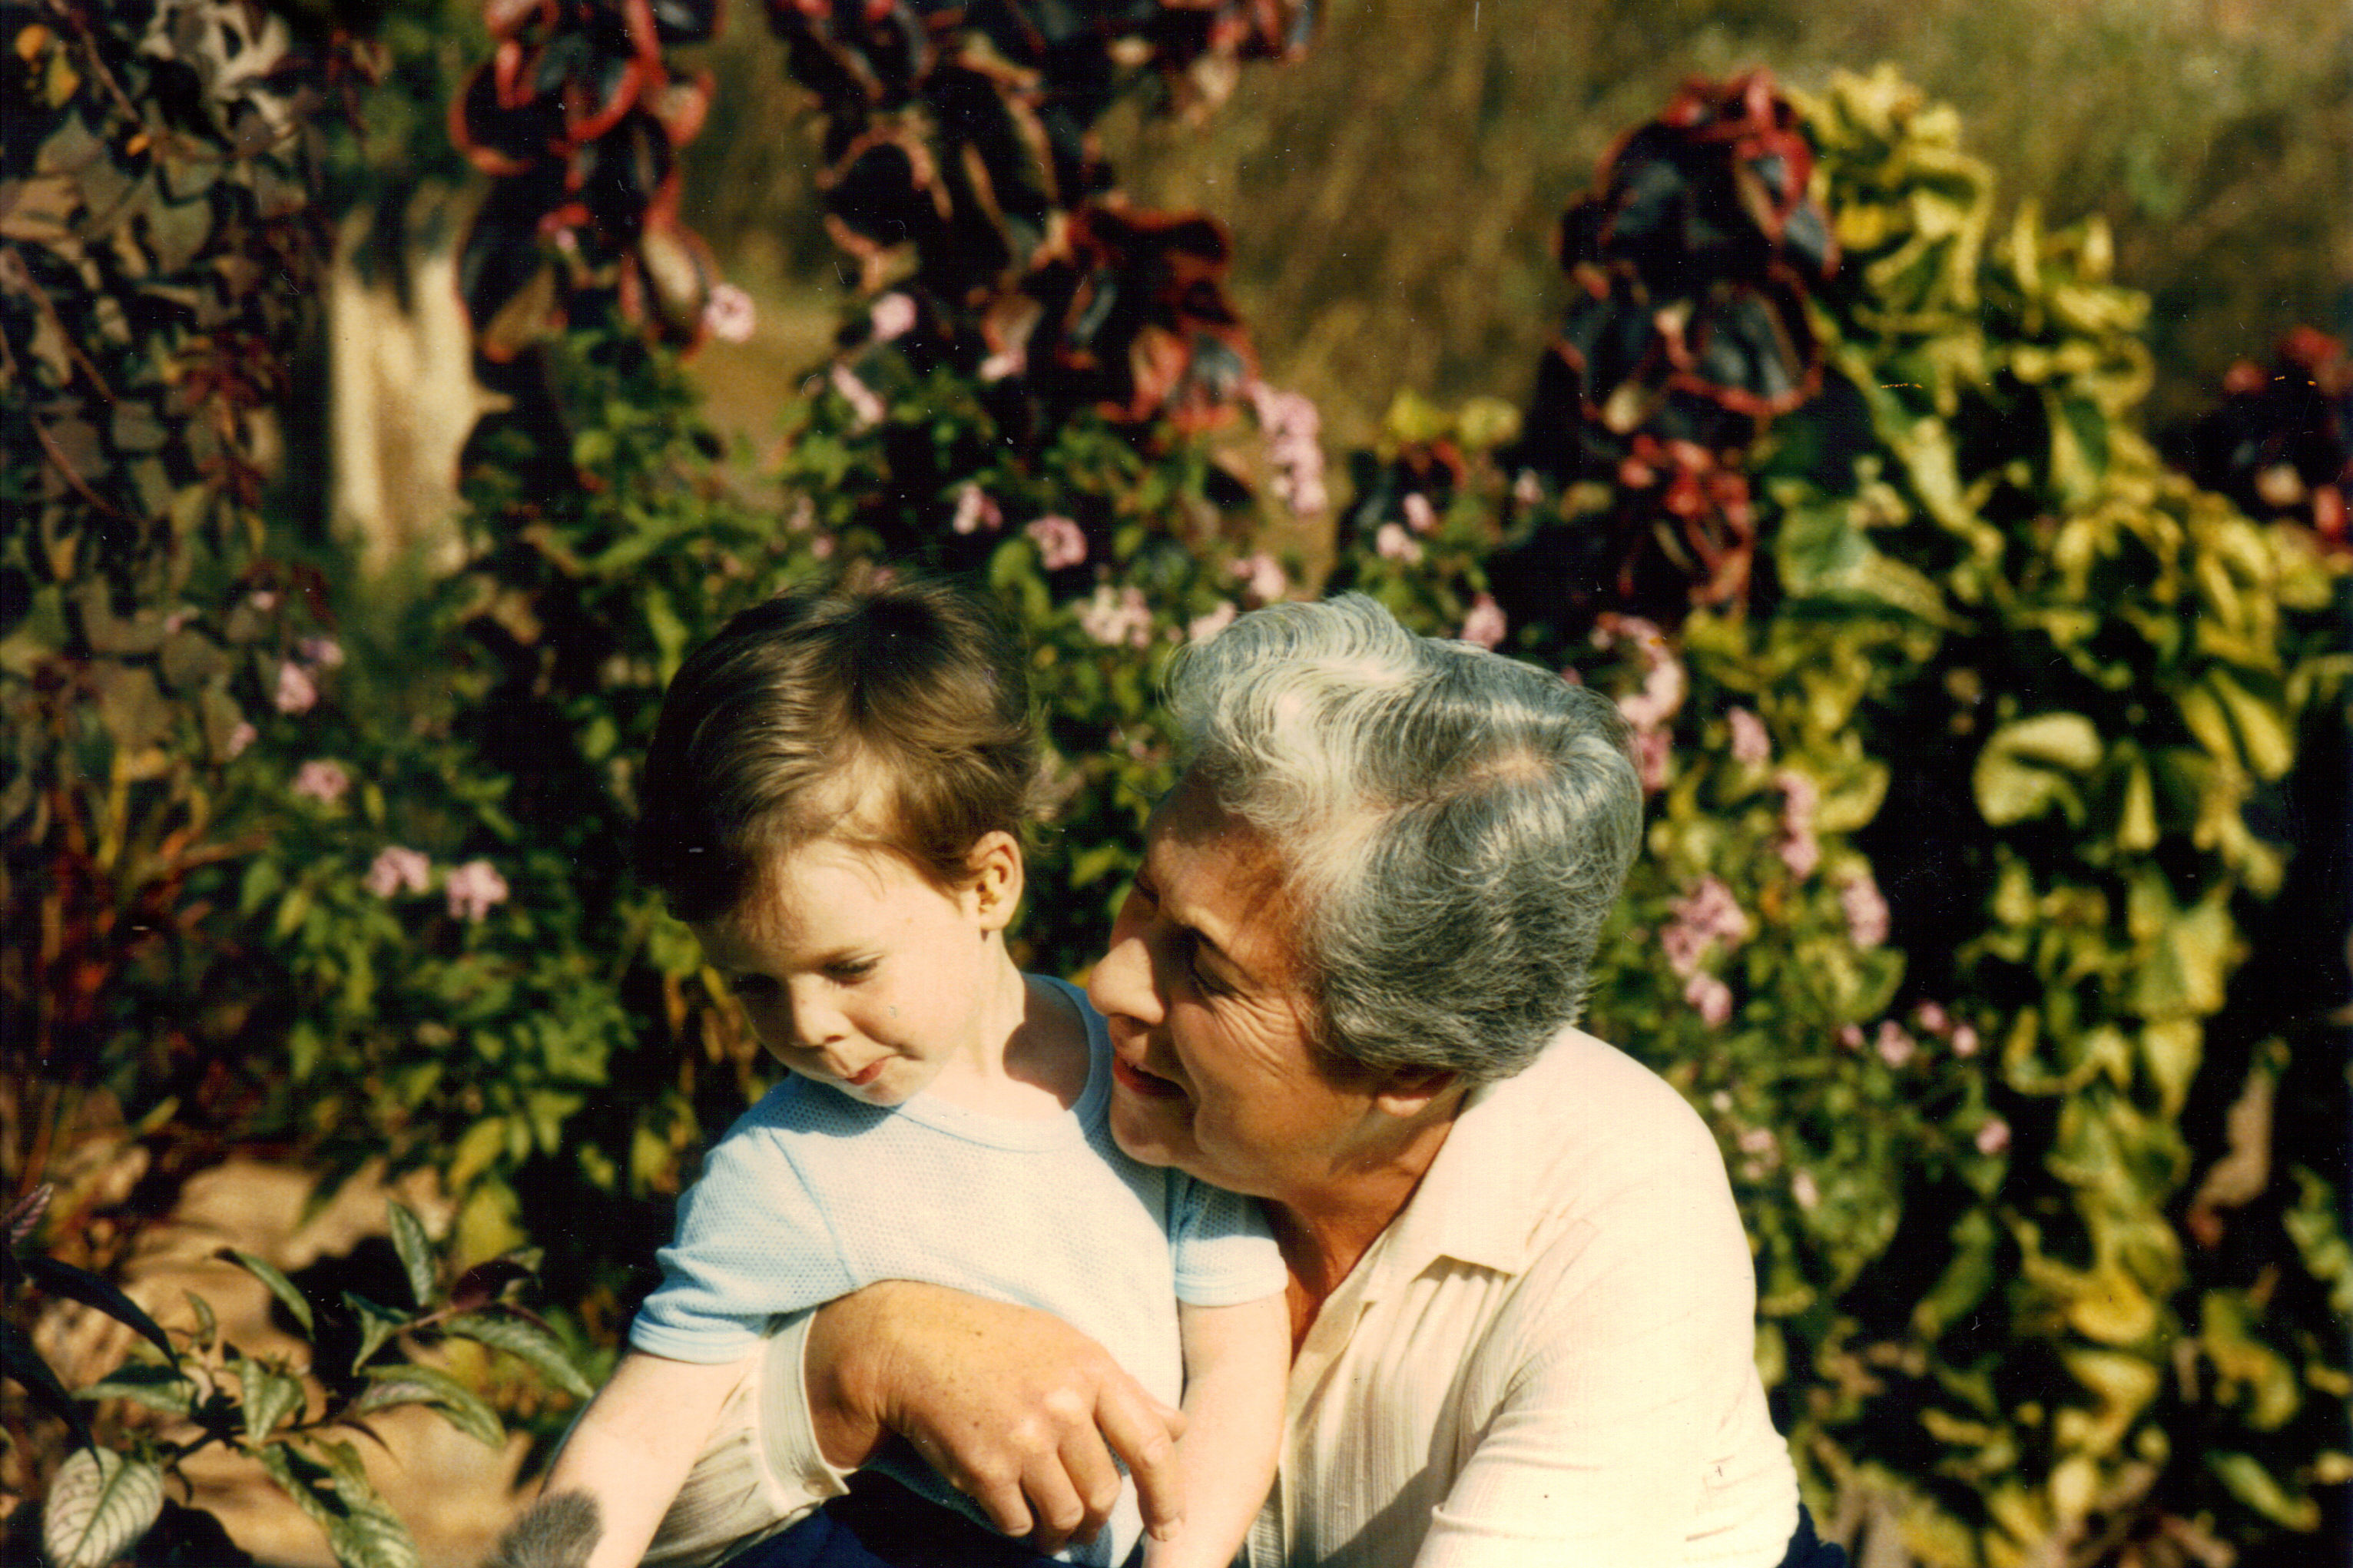
\includegraphics[width=0.9\textwidth]{photos/madge-and-andrew.jpg}
  \caption{Madge holding Andrew.}
  \label{madge-and-andrew}
\end{figure}

This reminds me of another time when I was giving my mother a home
perm. Because I hadn't been concentrating and had omitted one vital
procedure, I had to start all over again. ``Read the instructions
Grandma'' -- Andrew was quite right!

On another occasion I was trying to change the nappy of a very cross
and spirited Claire and I couldn't cope with her screams and kicking
legs. Andrew said ``Move over, Grandma, I can handle this.'' And so he
did with practiced ease.

He must have thought me a real dimwit at times but he never held it
against me. It was interesting for Tony and me to follow his progress
through school and toward adulthood. He achieved his BSc. in 2005 and
then moved on to his PhD without having to write his Masters.

Tony, being of a mathematical mind, was so proud of Andrew and they
had some serious discussions. What a good thing that he took some of
Tony's brains and not mine.

How lucky I am that he and Shaun have got my memoirs into shape to
produce an attractive -- and I hope readable -- book. He is launched
into a successful career but it is beyond me to understand exactly
what he is doing!

Claire is next in line for comment. She was a beautiful girl -- and
still is. We got on very well until things went sadly wrong. The
family had spent the day with us in Winston Park and, for some reason,
Claire chose to spend the night with us and we made up a bed for her
in our bedroom. We were woken up by the sound of a very loud
howl. Claire was sitting up in bed, clearly distressed and not knowing
where she was -- poor little thing. After a drink and some comfort I
took her into bed with me -- I don't know what we did with grandpa --
but the rest of the night was most uncomfortable for she kicked and
fidgeted and I was thoroughly glad to see the morning!

That was the beginning and end of Claire's nocturnal visits but she
remained very precious. Her visit to me in 2012 is so memorable; she
came with Tom (her longtime boyfriend) and, of course, Elizabeth and
we spent some lovely times together, especially during the week we had
in the Drakensberg. We certainly had some wonderful laughs. Claire
schooled me in playing DVDs and CDs but I have never rid myself of
being afraid of doing something wrong with the equipment.

It does not help to realize that I belong to the lost generation of
computer illiterates but we haven't done too badly.

I have found Claire to be a light-hearted, fun-loving, and extremely
practical girl. I am sure she could lift anyone's low spirits and I
hope that sunshine will always be with her; I feel she will never lose
the ability to bring this and happiness into other peoples' lives.

In time Lisa, another beauty, arrived and I enjoyed babysitting with
her. In those early days, we seemed to develop a rapport. Partly, I
think, because of the lullaby I sang to her when she was
unhappy. Always the same tune, ``Wouldn't it be Luverly,'' from My
Fair Lady. She would stop her nonsense and look up at me. She seemed
to recognize the tune and her little eyelids would close. I was very
happy, not only because she had succumbed to sleep, but because the
song had become ours.

Lisa grew and blossomed and, in her teens, went to America on a
student exchange. Back in New Zealand she graduated from a 3 year
course at Victoria University of Wellington and, as I write, is
supremely happy in her first teaching job.

Shaun was 6~months old when the family emigrated to New Zealand so
babysitting with him was mainly watching him sleep; but there were
always his brothers and sisters to be played with or read to.

Tony and I were devastated when the family departed but luckily we
were able to visit them 4 times. But by the time we had re-established
relationships, it would be time for us to leave. We had nice visits
from them when they came for holidays to South Africa and it was good
then to get to know Shaun.

He seemed a very shy boy and I had almost given up hope of
conversations, etc., when, one evening, we were all together playing
some card game and the lights went out. The only thing left for us to
do was to enjoy the candlelight and talk -- and talk Shaun did.  He
was especially interested in talking to Tony and so began a good
rapport. Praise be for electricity failures!

Shaun has not yet decided on a career but he is a good sportsman and
is a fabulous footballer. Who knows? That may even become his career.

\begin{figure}
  \centering
  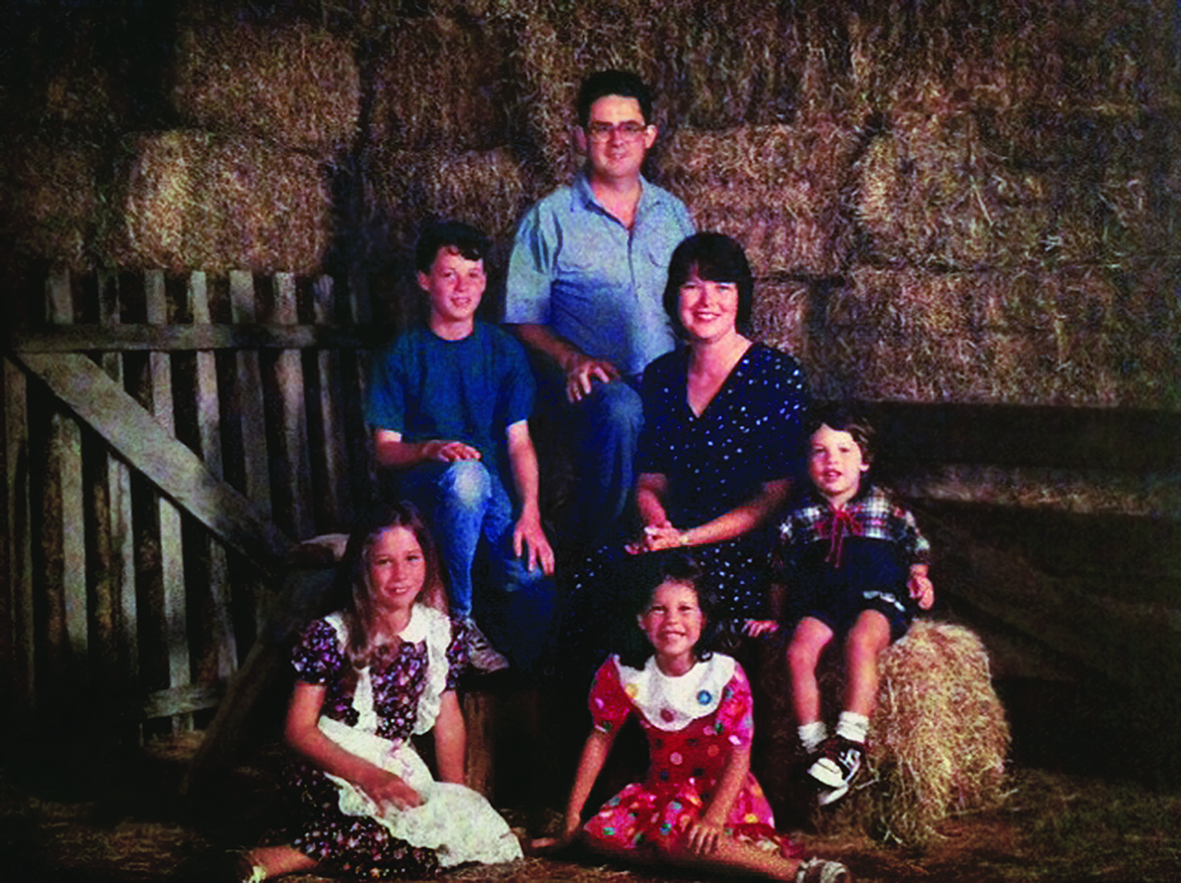
\includegraphics[width=0.9\textwidth]{photos/preston-family.jpg}
  \caption{The Preston family (Rotorua, 1995).}
  \label{preston-family}
\end{figure}

We missed the Preston family terribly when they departed to foreign
shores (see Picture~\ref{preston-family}) but were were not entirely
deprived of grandchildrens' company. We enjoyed the visits of Ryan and
Kelly-Ann (Richard's children) who were living with their mother in
White River. Because of distance we had not seen much of them but we
began to enjoy having them stay during school holidays. It was a long
journey for them to come from White River; having been dropped off in
Johannesburg they then had to face the long bus journey to
Durban. They must have been 10 \& 8 for their first holiday with
us. We were allowed to use a holiday home at Uvongo -- courtesy of
Dave and Muriel Harris -- and we all loved being by the sea for
2~weeks of each holiday (see Picture~\ref{ryan-kelly-ann}).

\begin{figure}
  \centering
  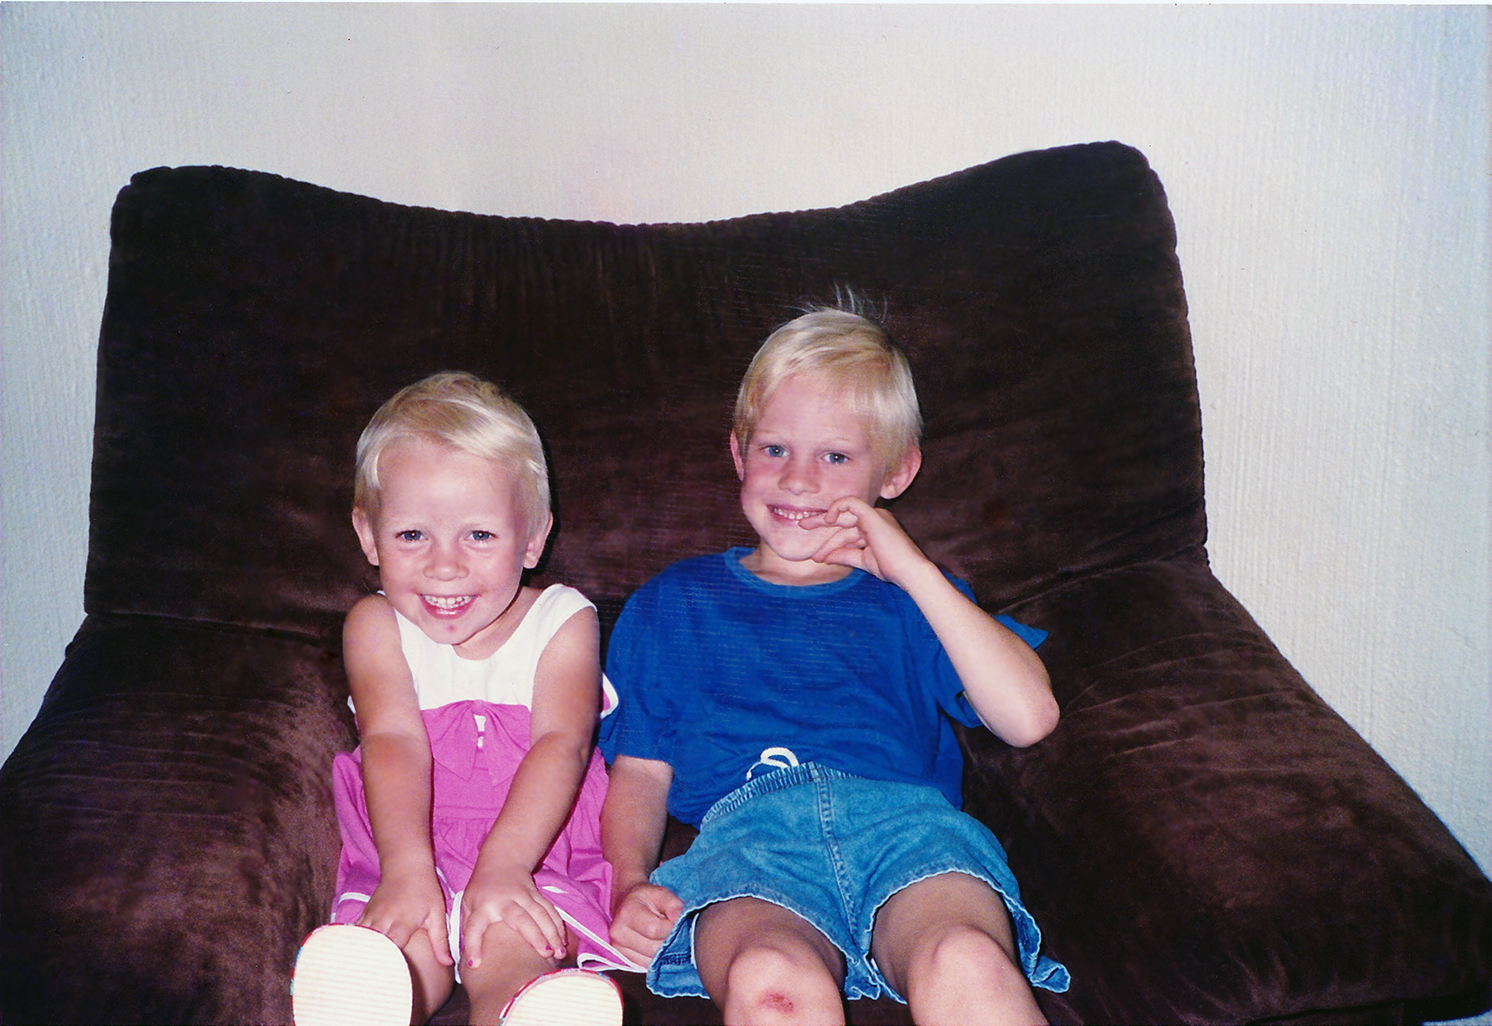
\includegraphics[width=0.9\textwidth]{photos/ryan-and-kelly-ann.jpg}
  \caption{Ryan and Kelly-Ann (1993).}
  \label{ryan-kelly-ann}
\end{figure}

Tony and I would sit and watch them -- rather like Darby and Joan --
when they climbed of rocks catching crabs and loving the sound and
sight of the sea crashing over them (this held quite a bit of
trepidation for me). They were a quarrelsome pair and when we arrived
back home they would fight over who was to have the use of our one and
only electric blanket. Evenings were spent playing Backgammon and they
were very helpful around the house. They had been very well trained by
their mother, Hazel.

We often cooked pancakes establishing a sort of conveyor belt system
with the tossing, adding sugar, and rolling process. It was great fun;
incidentally this cooking fun has also been enjoyed by the Preston
children and, as a matter of fact, by children who wandered into my
kitching in Lagos. There is something about pancakes!

Ryan was boisterous being a boy and we all joined in playing
cricket. He and I played table tennis and I never succeeded in beating
him!

Kelly-Ann was quiet, poised, and capable; I was amazed at her economy
of movement in whatever she was doing.

It was so sad to say goodbye to them and I shall never forget the
tears in their eyes when they pressed their faces to the window of the
departing bus. We have kept in touch as much as possible but phone
calls are not the same as physical contact.

Making good progress through school, Ryan went on to earn a degree in
all aspects of property development at Plymouth University in
England. He took part-time jobs to help with the financial side and
this made me feel very proud.

At university he met Natalie and they graduated together, afterwards
moving to Dubai where they both found good jobs. They are to be
married in Cape Town in March 2014 and I hope to be able to go to the
wedding and to watch the beginning of the greatest adventure of all
time.

Kelly-Ann stays in White River and is working as a swimming
instructor. She has produced a baby girl -- Anne -- my first great
grandchild whom I hope to meet at the wedding.

And so to the children of Richard's second marriage -- Robin (Pat's
son) and Bradley (see Picture~\ref{richard-family}). Robin is making
fantastic progress in the hotel industry; having trained at the Mount
Nelson Hotel in Cape Town, he is now a member of the staff. He is a
real ``peoples person'' with his charm and personality and Tony and I
grew fond of him albeit that we have not had the necessary personal
contact. I am sure he has a great future.

\begin{figure}
  \centering
  \includegraphics[width=0.9\textwidth]{photos/richard-family.jpg}
  \caption{Richard, Pat, Robin, and Bradley (Cape Town, 2013).}
  \label{richard-family}
\end{figure}

Bradley is making good progress through school. Once more there has
been little personal contact but we have had wonderful chats over the
phone. He has a lively and charming personality. It seems highly
possible that he will enter the hotel industry and I wish him luck.
He has an amazing ability to absorb information and to impart it and I
am sure he will become an excellent hotelier.  Good luck, Bradley.


\chapter{Nigeria}

Nigeria lies 6 degrees north of the equator.

It took a while to get used to the unpleasant conditions. The
temperature being around 30 degrees celsius for almost the entire year
and the humidity 80~--~90\%; there was little relief during the night
time but we were fortunate enough to have air-conditioning in the
bedrooms of the lovely house we occupied during our 11 years there
(see Picture~\ref{family-nigeria}).

\begin{figure}
  \centering
  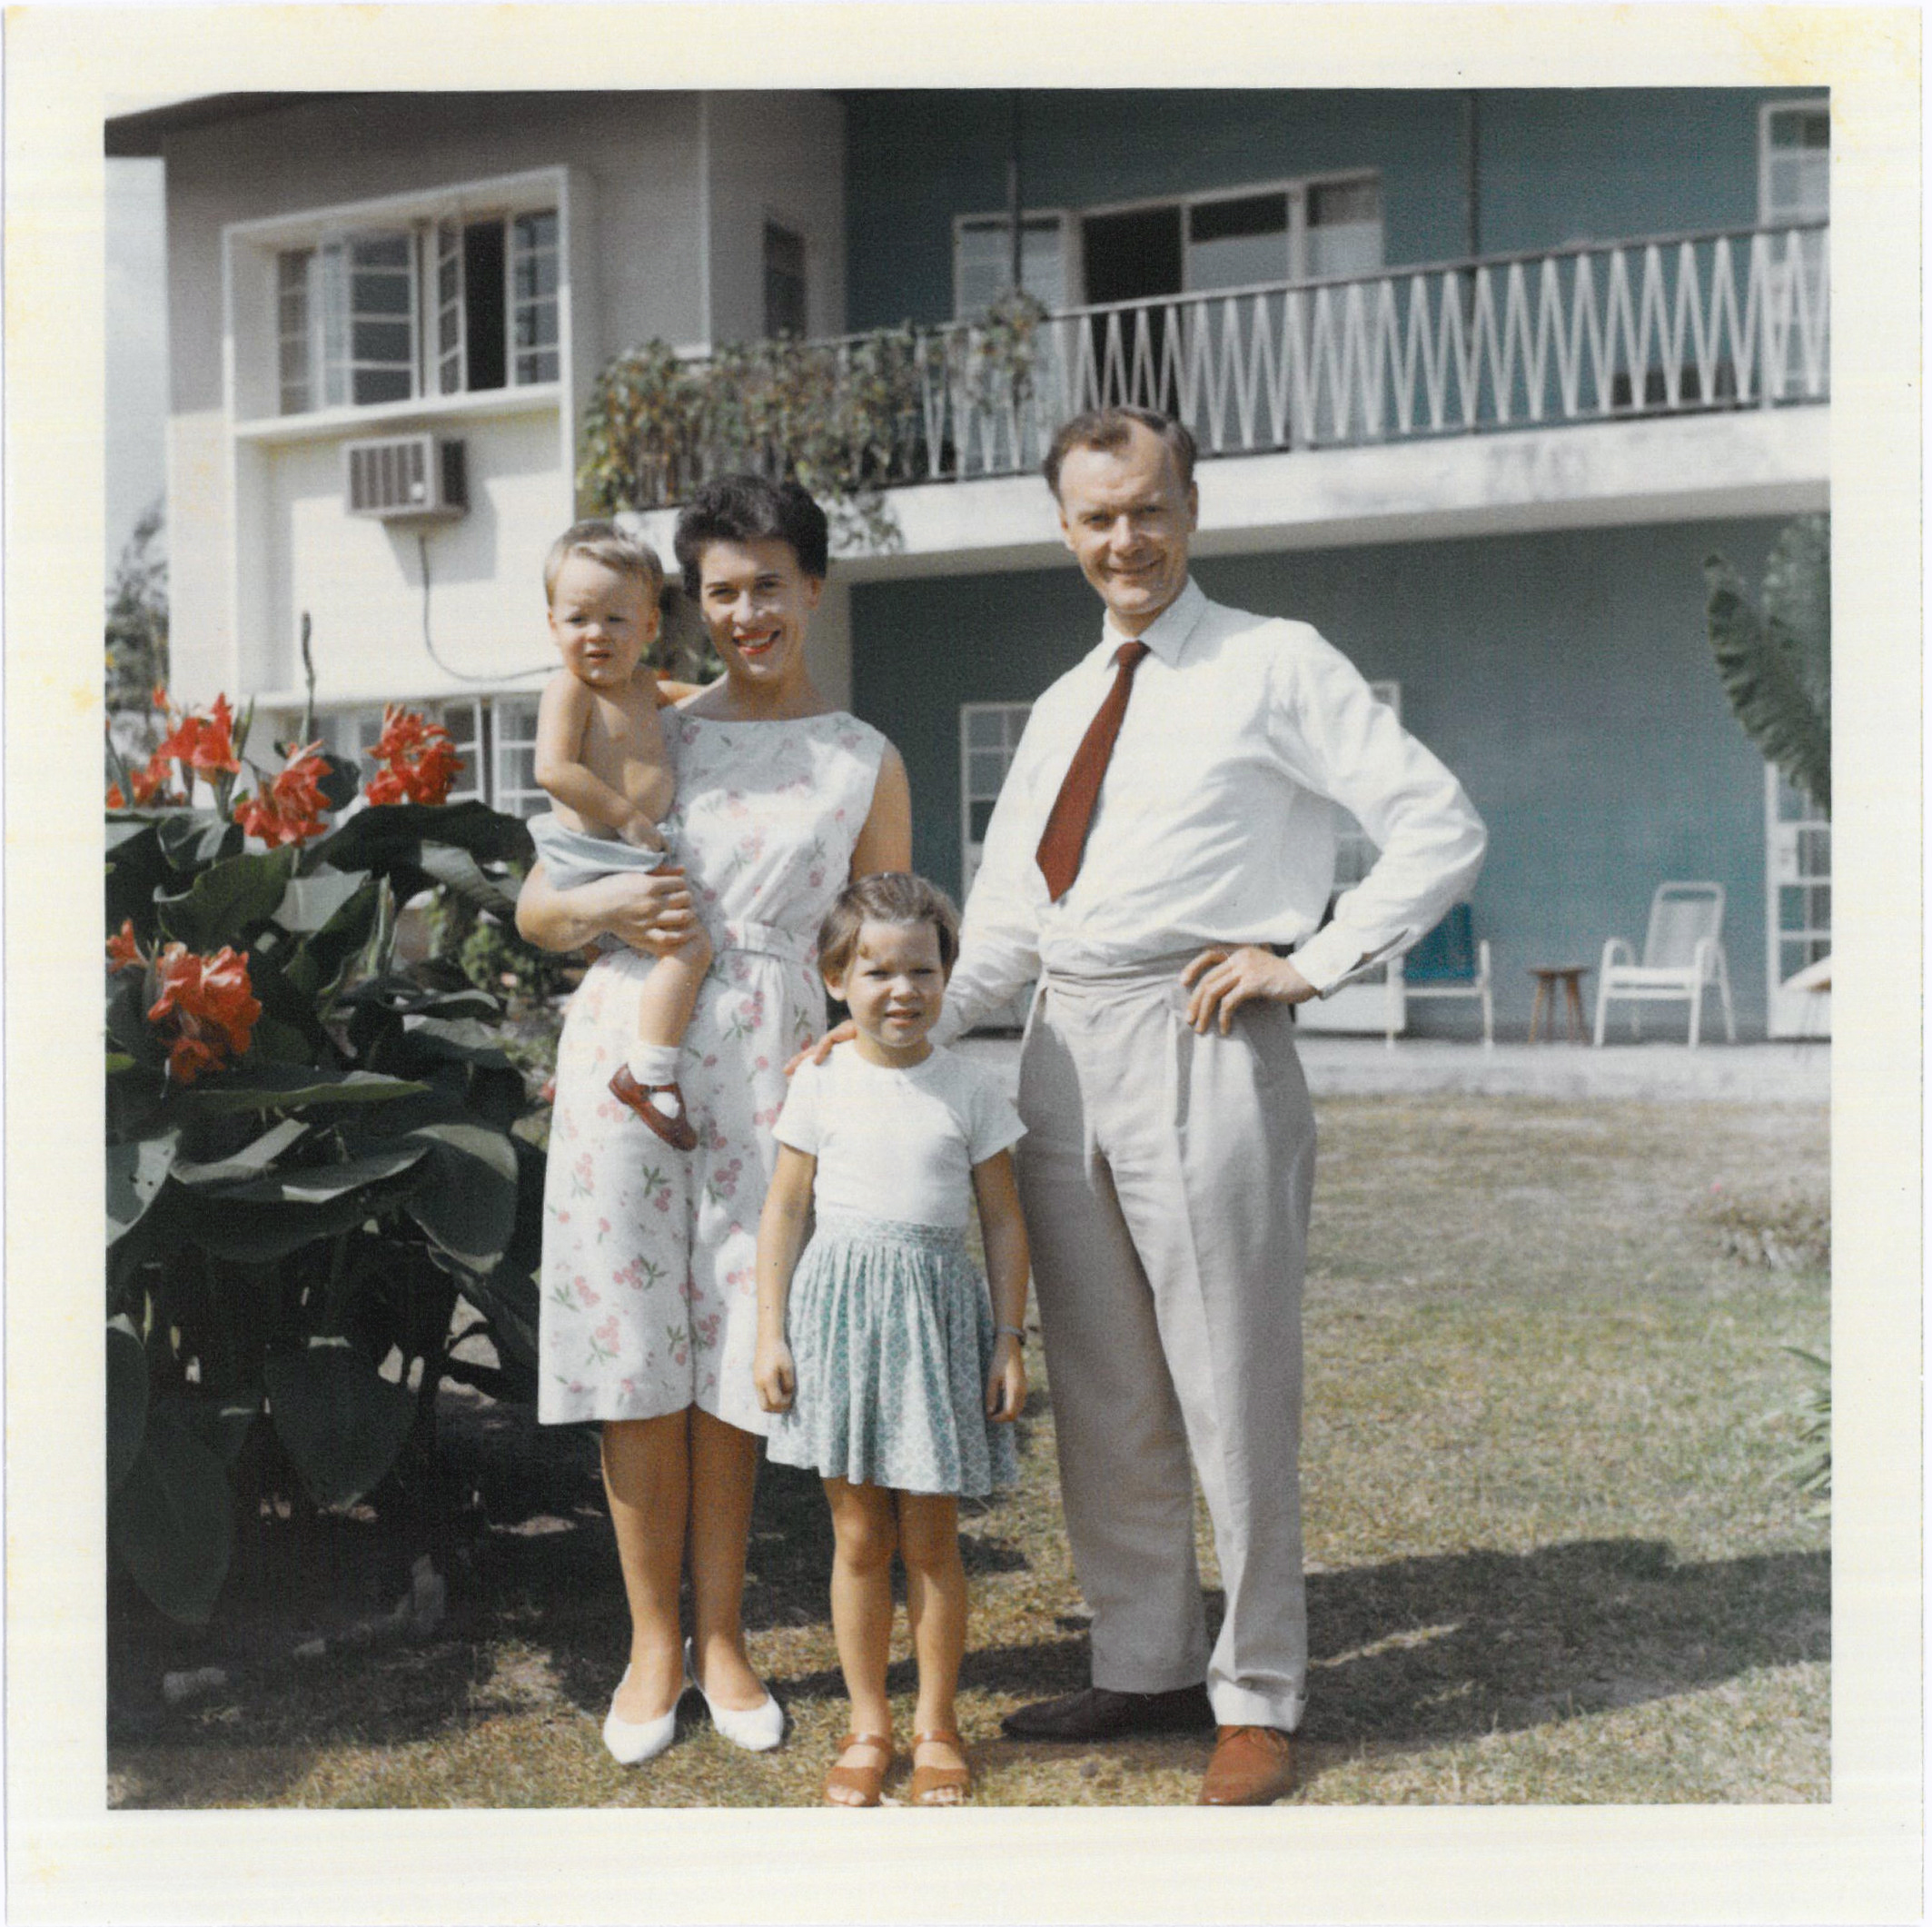
\includegraphics[width=\textwidth]{photos/family-nigeria.jpg}
  \caption{Tony, Madge, Elizabeth, and Richard in front of their house
  in Lagos (1965).}
  \label{family-nigeria}
\end{figure}

With Nigerianisation maintenance of basic services like electricity,
water, etc. fell away and sometimes we would experience cuts of 72
hours. I am pleased to say that, in spite of the lengthy electricity
cuts we only ever lost six ice lollies! And in spite of Audu (our
faithful Muslim cook/steward) opening the fridge door to discuss lunch
not realizing that one gust of that hot humid air would spoil the
contents or cause defrosting.

Audu and I became great friends and would often have discussions about
things in general. He was a good ``all rounder'', even taking an
interest in the garden. He was tall and of good bearing and came from
the north. He belonged to the Hausa Tribe.

He was mystified about the immaculate conception -- ``You know how you
borned Elizabeth. Ma'am.''

I did find things difficult to explain sometimes.

Audu was a good cook and laundry boy.

We would discuss the menu for a dinner party, in spite of his
intelligence, if I forgot to mention some condiment, he would not
include it -- e.g. If I did not mention roast potatoes, they would be
excluded from the roast lamb dinner!

I remember that there was a succession of ``small'' boys (A small boy
would do the cleaning etc: one boy who suffered with B.O. and this was
so overpowering at times that he had to be told to shower and change
his clothes, he would come back smelling of roses but not for long!)

Around December time a wind -- the Harmattan -- would blow off the
Sahara and deposit sand on floors and furniture etc: furniture had to
be dusted several times a day but this was pointless. It was almost a
relief to escape this dry air and get back to the heat and
humidity. The dryness would bring sinus, cough and chest problems. And
I had a problem which was not helped by my pregnancy as I was now
expecting Richard and the early part of 1964 was not pleasing for me.

I did not want to be in the air conditioning during the day times and
I enjoyed sitting in the garden. We overlooked a creek (were we up the
creek without a paddle?!) and then over an island was the Atlantic. We
had the illusion of cool breezes coming off the ocean. It is known as
``the breeze factor'' and it was very comforting.

\begin{figure}
  \centering
  \subfloat{
    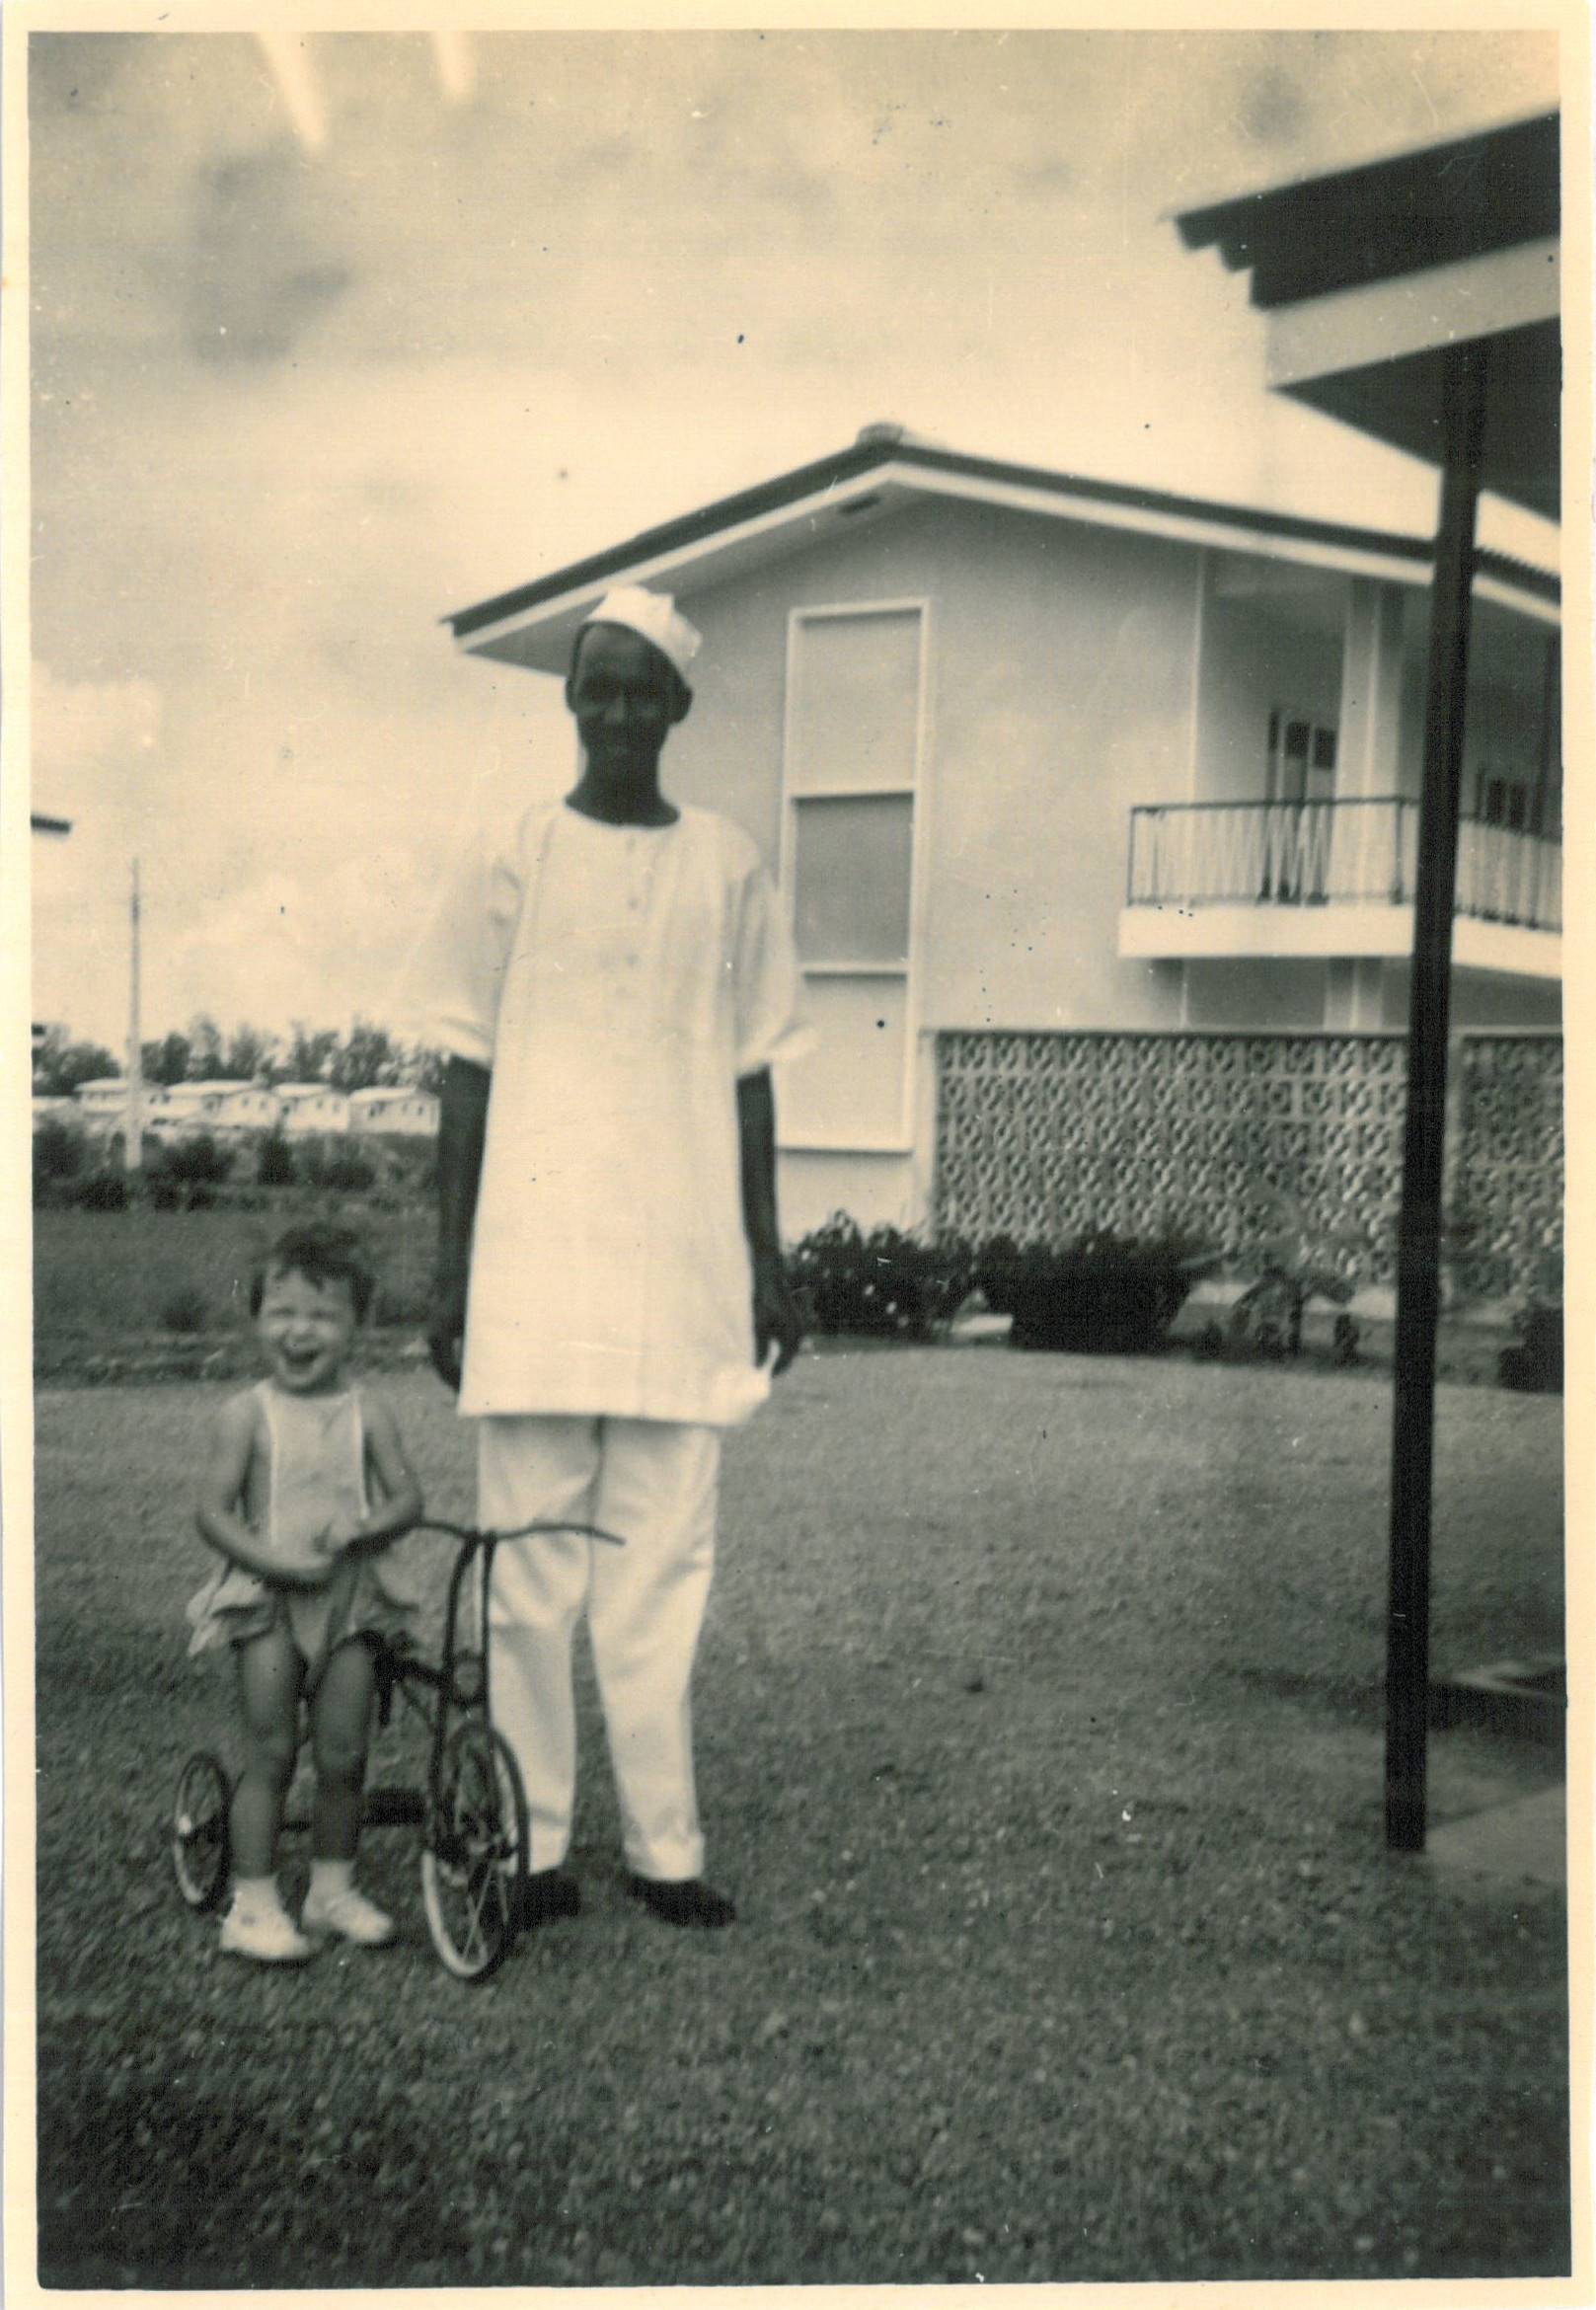
\includegraphics[width=0.45\textwidth]{photos/elizabeth-with-audu.jpg}
    \label{elizabeth-with-audu}
  }
  \subfloat{
    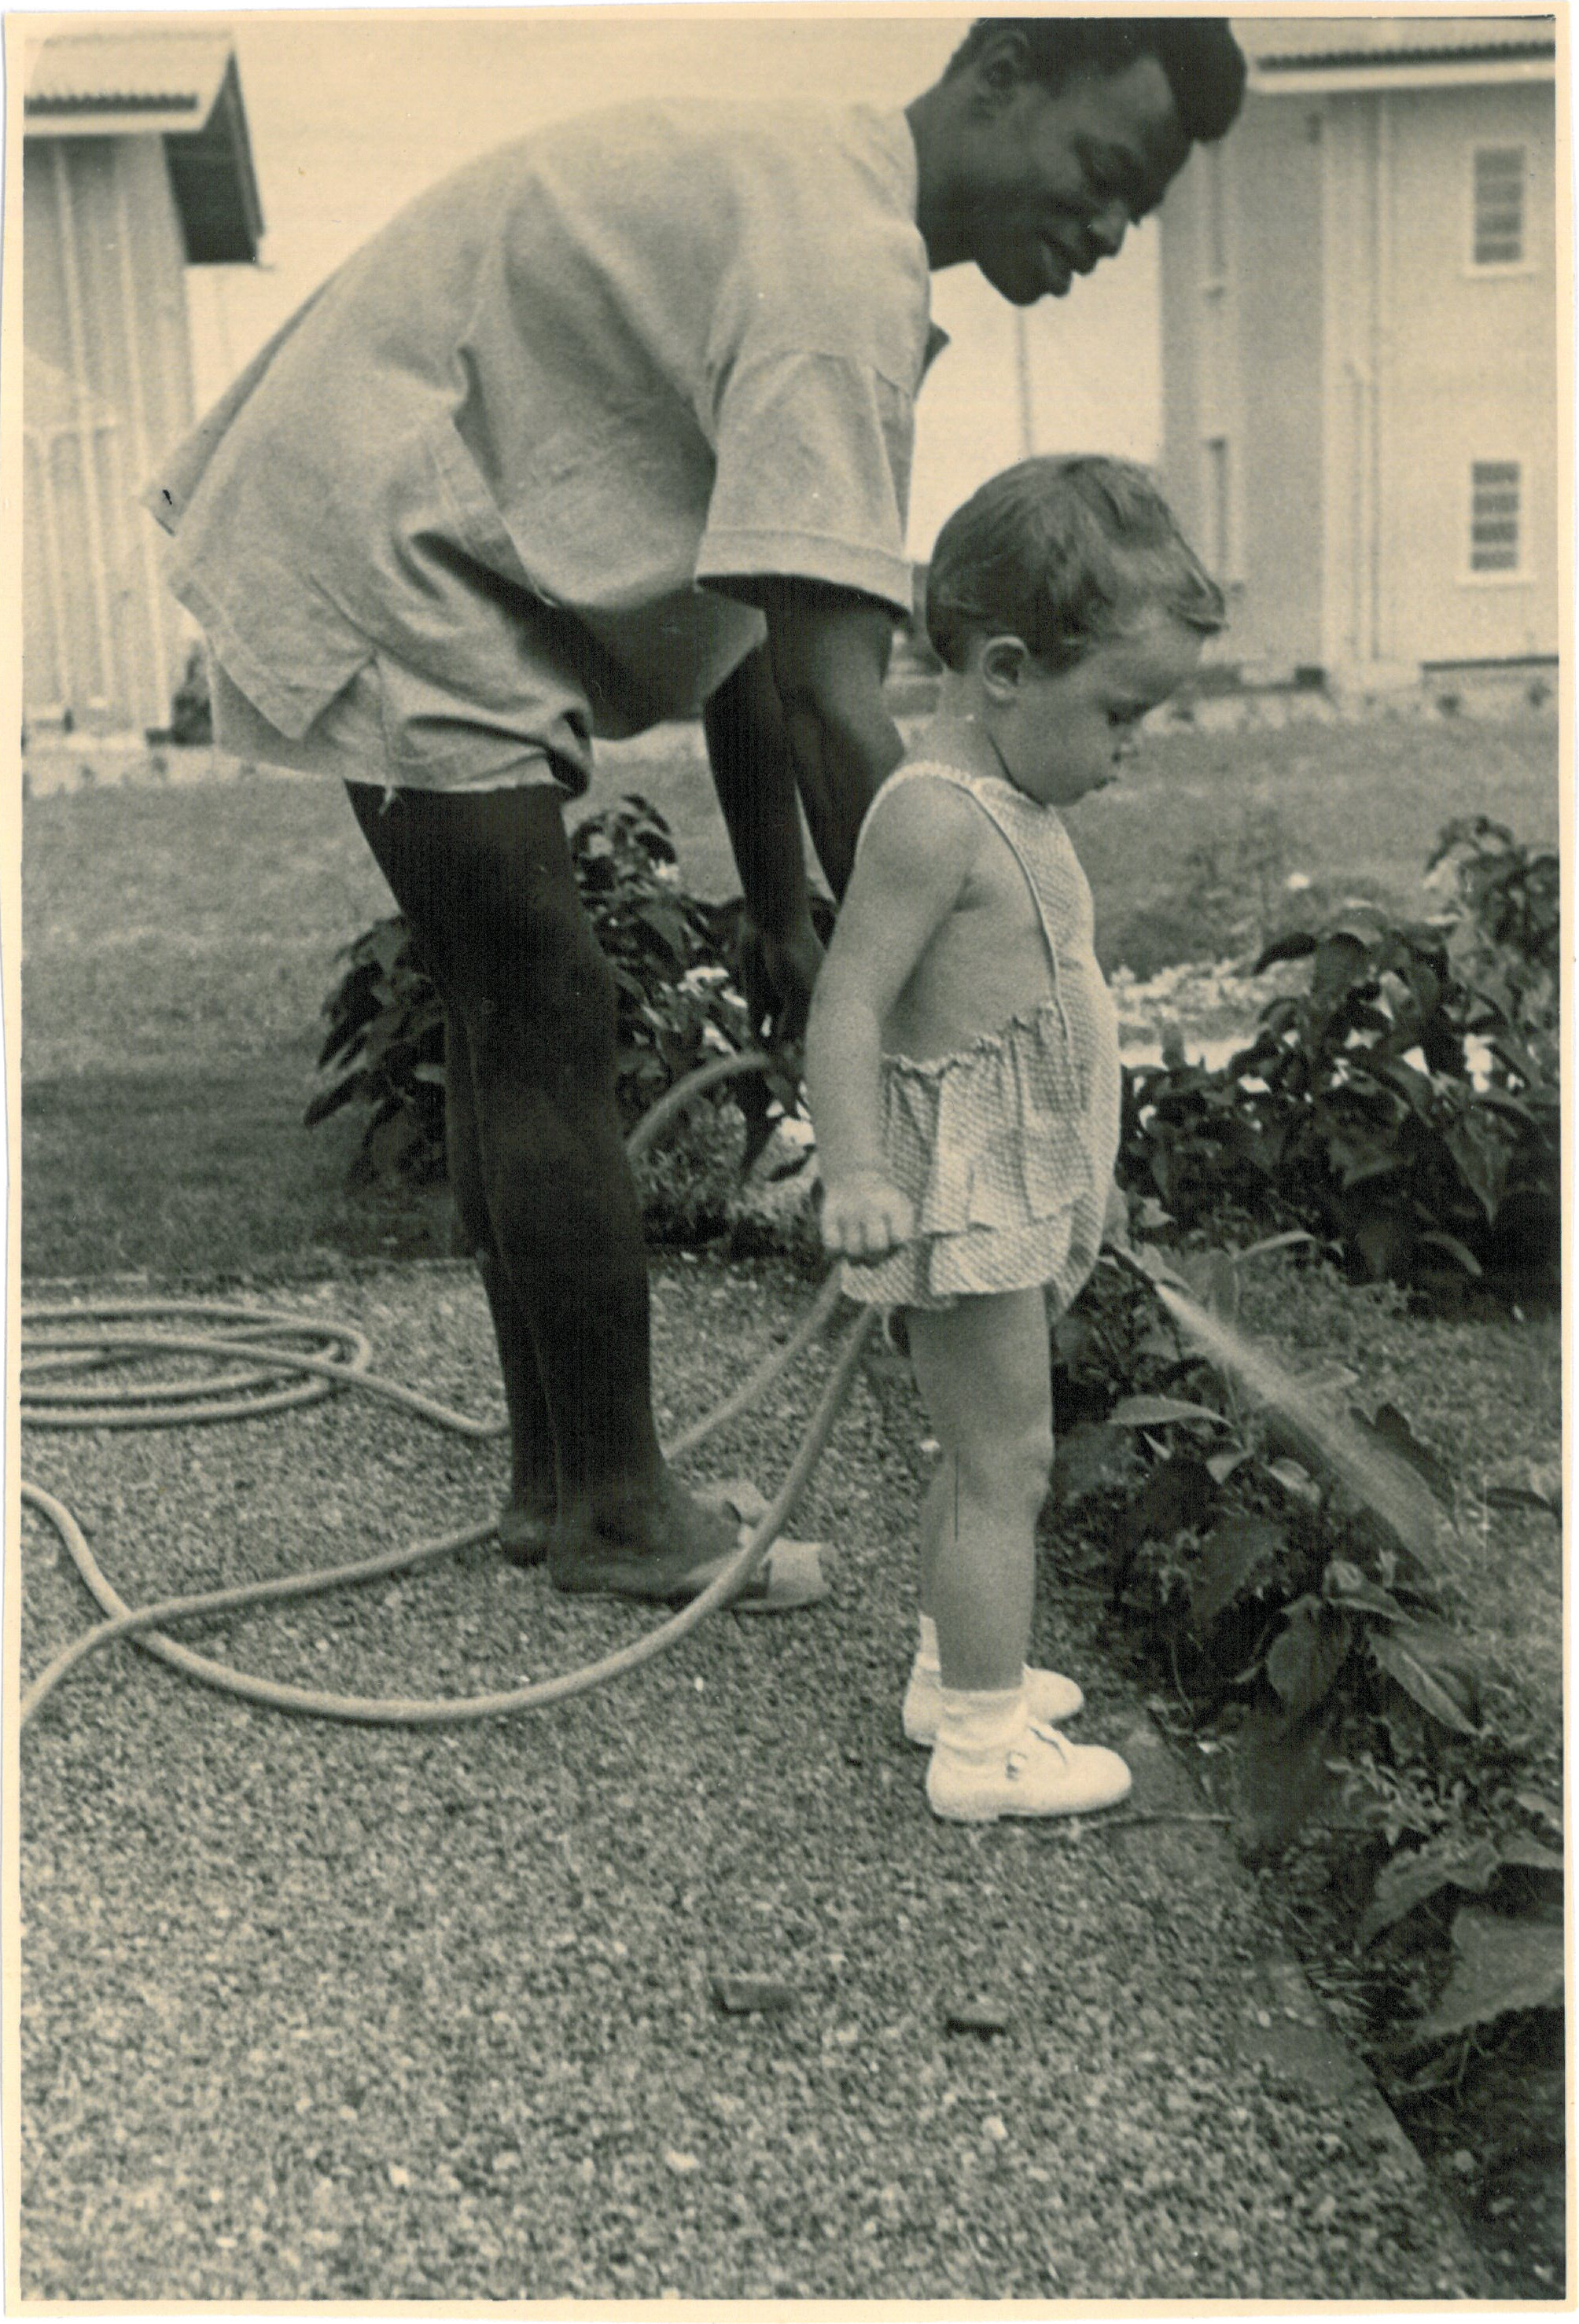
\includegraphics[width=0.45\textwidth]{photos/elizabeth-with-gardener.jpg}
    \label{elizabeth-with-gardener}
  }
  \caption{Elizabeth with (left) Audu and (right) Andrew (Lagos,
    1962).}
\end{figure}

There was a large expatriate community in Lagos and we made many
friends, particularly, in my case, of women. I became a colonial wife;
there were countless tea and coffee parties and we would vie with each
other to produce the biggest variety of cakes etc. How silly! But it
helped to pass the time! I smoked in those days too, to be social. How
very silly!

I did a lot of sewing in those days and I would be at the sewing
machine by 8~am, until Elizabeth came home from school (our chauffeur
would take her). I can hardly believe that I did not get out of bed
before 8~am, by which time Tony had had his breakfast and gone to
work.

My hobbies have always been of the needlework variety -- sewing,
knitting, embroidery, dressmaking, etc. My first attempt at embroidery
was of a bunch of daffodils on a tray cloth. In the making I took it
with me when I went to stay with my grandmother. I think I was about
twelve. I was ``caught'' working on it on a Sunday morning and I was
in real trouble. Sewing in the morning when there are jobs to be done
and on a Sunday too! Whatever next?!

I must have learned the basics of sewing at school and I knitted
during college days but it was not until we got to Nigeria that I
started to sew ``seriously''. I found a hundred-year-old Singer sewing
machine waiting for me when I arrived in Lagos with Elizabeth. Tony
had acquired it (I thought you might like to make curtains for the
house. Goodness! Full-length and lined -- a learning curve indeed!)

I had to cut the curtain out on the floor because of their size and
the iron was handy. We were very amused when Elizabeth told Grandpa
that she had to be careful not to burn her ``botham'' (bosom).

The machine did wonders for me and it was thoroughly used to make
clothes for the children and myself. It is likely to survive several
more hundred years because of its unique sturdiness.

Being a ``colonial'' wife I had time on my hands and I started to sew
at 9am! Clothes for Elizabeth, Richard, and myself. My great joy was
to make something out of something else -- my triumph was four
maternity smocks out of two dresses; and a friend gave me eight
cast-off dresses of her daughters for me to alter and make dresses for
Elizabeth. Which turned out very well indeed. Also I used Tony's
discarded white ``sea-island'' cotton shirts to make shirts for
Richard -- wonderful material -- and, by placing the pattern so that
the existing button-holes were in the right place, the finished
article managed to look professional!

``Make do and mend'' was a slogan we learned during the war and has
always stayed with me -- although I think I probably inherited my
thrifty ways from Grandmother.

I loved mending and I even managed to be complimented by my
mother-in-law on my darning of Tony's socks! I mended a lot of
Elizabeth's childrens' clothes, even toys, and got a great kick out of
that. By the way, the sewing machine stayed with me and saw more years
of sewing in South Africa until I finally gave it away to the maid of
a friend who thought she had inherited the crown jewels!

I once went to Bristol after finishing college and saw a table cloth
in a needlework shop window. It was made of Irish linen and huge
transfers were in place. There was, obviously, a lot of work to be
done. This was the reason it had been reduced in price (its original
price was 29/11 and down to 9/11). I had to have it.

I only started work on it when we were in Turkey and it took me a
whole year to finish. It helped me through many long hours of being
alone and waiting for Tony to come back from work -- such rewarding
work. It has been used (and laundered. Oh my! What a task). I have
passed it on to Elizabeth and I hope it will be used. It is something
of an heirloom and I have embroidered my name and the date in the hem.

Audu would do the routine cooking and laundry work -- and Edward the
cleaning -- and so my mornings were taken up with sewing, coffee
parties and my special ``Goodies'' for lunch and dinner parties
etc. How this was to change when we got to Johannesburg and I had no
servants by choice. But that was to be 11 years in the future and life
in Nigereia was there to be enjoyed, sometimes hated and found to be
frustrating but nonetheless part of ``Life's Tapestry''. I had to go
back to Engalnd to have Richard in 1964 and we were delighted because
he now completed the family. Elizabeth was the perfect 4-year-old
mother and looked after him when I had to go out -- of course, Audu
was always there at these times. Things could get out of hand. If
Elizabeth tried to change a nappy, it would finish up around Richard's
ankles and once, when he was thirsty, she gave him lime juice which
had disastrous consequences! But both children brought us much joy and
we were very blessed.

In 1966, the Biafran war started and this brought some unpleasant
experiences. The state of Biafra wanted to break away from the Federal
Government and took up arms to support their cause. Differences in
Lagos were strong but people would try and live normally. We would
drive to dinner parties leaving the children with Audu -- an excellent
baby-sitter -- and be stopped on the road by a soldier -- either drunk
or drugged -- and Tony would be questioned about whether he was
carrying weapons etc., and we would both be frightened by the
demeanour of the soldier. ``Please God, let us get back to our kids''
I would pray silently.

In 1966 we had a first-hand share of the war. Tony had to go to Ghana
for just one night and that was the ``Night of the Aeroplane.'' Eleven
of the Biafran rebels hijacked a ``Fokker Friendship''
aircraft,\footnote{The Fokker F27 Friendship 5N-AAV operated by
  Nigerian Airways was hijacked on October 7, 1967, while \textit{en
    route} from Benin to Lagos. See
  \href{http://www.mercenary-wars.net/biafra/index.html}{http://www.mercenary-wars.net/biafra/index.html}
  and
  \href{http://news.google.com/newspapers?nid=1774&dat=19671007&id=Pn4fAAAAIBAJ&sjid=6mUEAAAAIBAJ&pg=7328,1581485}{Picture~\ref{hijacking}}.
} loaded it with dustbins filled with explosives, and flew to Lagos in
the hope, it was thought, of blowing up the home of the president
(Jacobu Gowan) and government buildings. Something must have gone
sadly wrong because, instead of the dustbins being pushed out of the
plane, they blew up in mid air -- immediately above our house as it
happened. The children were with me in our bedroom and the bottom fell
out of Richards cot which landed him on the floor. He looked at me as
if to say ``What the devil is going on?'' The noise of the explosion
was terrific and I was more terrified than at any time during the
second world war. Small pieces of the plane were falling on the roof
and sounded like fire -- I was convinced that we were
trapped. However, we got downstairs and neighbours called. Windows had
been blown out and there was glass everywhere. I forgot to put on a
dressing gown but it didn’t worry me that Wally, our Australian
neighbor, showed a particular interest in me and my flimsy nightie!
There were body parts scattered over the garden and Wally found what
he thought was a flying glove but was actually a complete Negro scalp!
We made tea (of course).

\begin{figure}
  \centering
  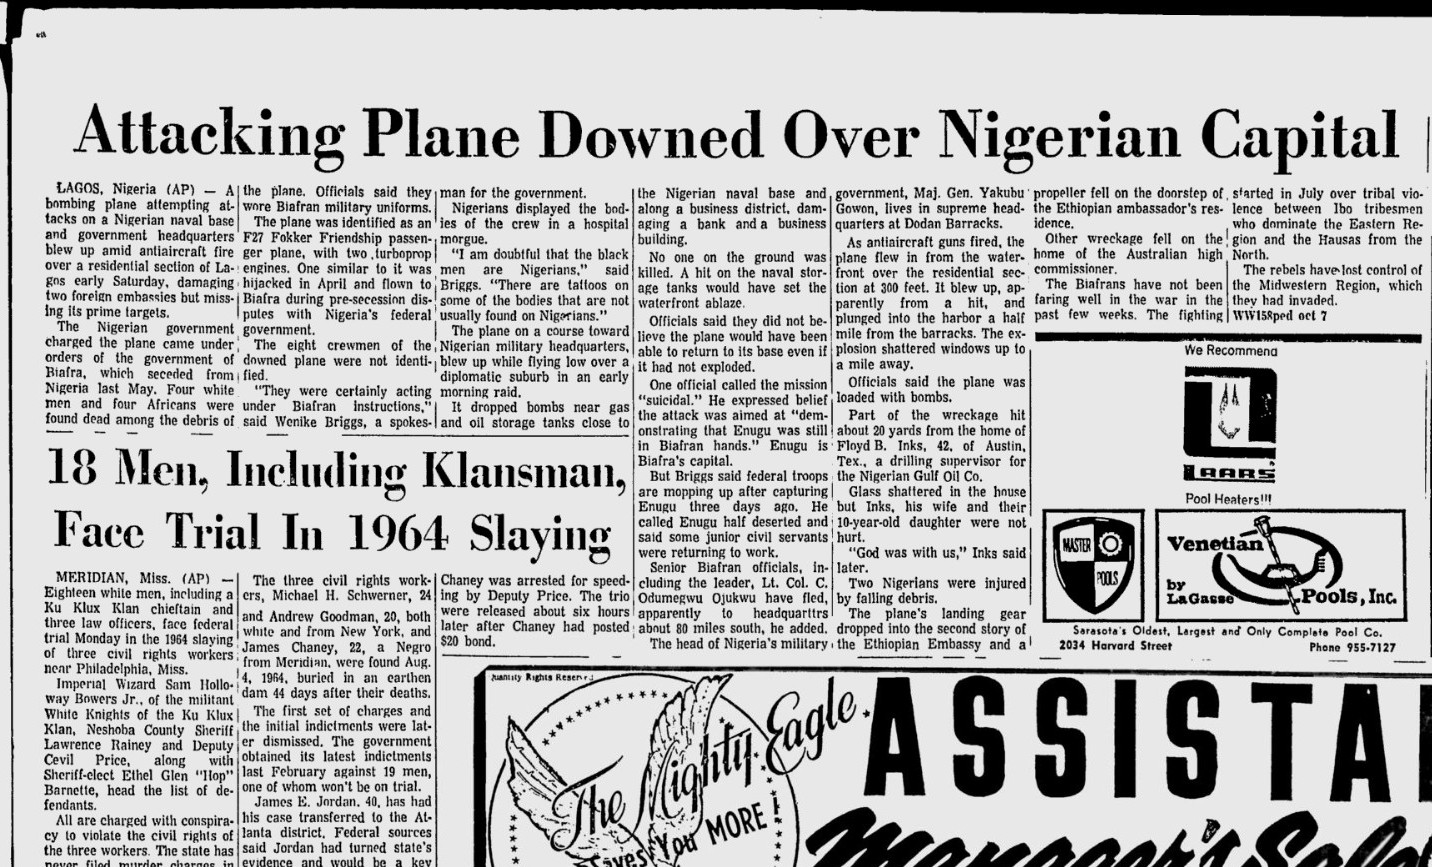
\includegraphics[width=\textwidth]{photos/nigeria1.jpg}
  \caption{From the October 7th, 1967 edition of the Sarasota
    Herald-Tribune.}
  \label{hijacking}
\end{figure}

We went back to bed but sleep was impossible, the morning light
brought sights to behold with brains hanging on bushes and complete
chaos. But that could have been much worse for the plane itself had
crashed into the creek. However, one of the doors had slid down the
side of our house and part of a wing had come through the roof. It was
raining so that made things rather inconvenient! Another wing had come
through the Weber's roof and landed on Nicola's bed. She would have
been killed if she had not gone to England with her mother the day
before. Her father (Ogy) had been to a party and got rather
drunk. When he came out of his bedroom and saw an arm and a hand on
the stairs he thought ``My God, I had more to drink than I thought I
had!'' But nobody was hurt which was a miracle. Tony returned to find
utter mess and chaos and it was only then that I gave way and burst
into tears. I had to have a course of vitamin B12 injections to get
over the trauma but things came right and somehow a sense of humor
persists and one is able to see the funny side of things
eventually. However it was not amusing for the director of the P~\&~T
to say to Tony ``A disaster to your family would have been no more
than you deserve.''

How racism rears its ugly head.

The Biafran rebels gained nothing from this escapade and I am not sure
if they ever managed to break away and gain their independence. There
were some in Nigeria (Nigerians) who said that Britain should never
have given that country its independence and I am of the belief that
most African countries have fallen flat on their faces and elected the
most incredibly awful, greedy, and incompetent leaders. I write this
in 2011 when we are witnessing the downfall of Egypt, Syria, and Libya
and starvation in Kenya and Somalia. But my thoughts are still in
Nigeria where we stayed for 11 years and we had a good life in spite
of the Biafran war. Luckily we had efficient guardian angels and I do
believe that I have had an army of guardian angels watching over me
throughout my life.

The memory of one will always be with me.

One day in 1966, when we were living in Lagos, I was persuaded,
against my better judgement, to spend the morning on a beach with
three of my friends and our combined number of 7 children. Elizabeth
was 6 and Richard 2. The beach was notoriously dangerous for having
claimed lives and, indeed, whole villages over a period of time. But,
nevertheless, it was a calm morning and not too hot. The two
Australian sons of our neighbours went into the sea and took Elizabeth
with them. All was well until a rogue wave came up to the shallows and
took the three kids out 6 feet. The boys' Australian mother, a strong
swimmer, went in to fetch them and I went in to fetch Elizabeth, which
was madness, as I can't swim -- even though I was born under the sign
of Cancer, a water sign. But I had to get my child -- there is nothing
as strong as the umbilical cord -- so there were now two of us
stranded in a restless sea. And then there appeared a man -- a
Nigerian -- dressed in the purest of white robes holding out a hand to
each of us. The sea parted and so he drew us to safety. The experience
must have lasted for 10 seconds but it seemed a lifetime.

Having drawn breath and being in the safety of the beach, I asked my
friends where that man had gone. But they denied any existence of such
a man ``No, Madge, there was no man here. You just walked out of the
sea.'' And it was useless to argue with them. We had been rescued by a
black man in the most dazzling of white robes -- beautiful to behold
-- my everlasting memory is of a guardian angel.

Thanks be to God.

Whilst we were in Nigeria (approximately 1970), cholera became endemic
and it is surprising that the disease had not gripped the country long
before -- perhaps it had but without World Health Organization
publicity.

Hygiene is a necessity in 3rd world countries but when a family has to
share a bucket of water (obtained with difficulty) it is not
surprising that such a disease can be easily transmitted.

Deaths occur because of severe dehydration. Once more we had to submit
to more injections and anyone coming into our house was ``invited'' to
wash their hands at the kitchen entrance. I checked up on Africans
through a peephole and called them to wash their hands if they had not
done so!

Once more, we were able to resist infection; in fact we had not
succumbed to other diseases there such as malaria, which is still
prevalent in the world.

Public executions for crimes such as murder, or even armed robbery,
were quite common and witnessing these events was very popular. And a
``day out'' with lots of excitement was very much welcomed by
thousands of people -- rather like going to the races. A popular venue
was close to our house and we could not help seeing the hordes
arriving; there was much excitement. We understood that refreshments
were available! Faintly we heard the gunshots ring out -- criminals
were strapped to fuel drums. Oh! It was horrible, but capital
punishment (perhaps administered more delicately) is necessary I
believe, and I can never see the point of keeping a violent criminal
alive to enjoy the comforts of a modern prison.


\chapter{South Africa}

Our lives in Nigeria continued until Tony accepted a position with the
GEC in South Africa. A year before we moved Elizabeth had reached the
age of 12 when there was no more schooling in Lagos and so she had to
go to boarding school in England (Wroxall Abbey). She was looked after
by Mandy Price who also attended the school and was the daughter of
Tony's boss Mel Price. We stayed with Mel and Audrey until the time
came to take the girls to school. My only thoughts on this day was
that Elizabeth would be away from us and in a different country. My
heart was heavy when we left her but there were no tears until bed
time when Tony said ``I was very proud of you today.'' I think my
heart burst and my tears soaked my pillow. Fortunately she was able to
fly out to us during the year and became a seasoned and confident
traveler. But oh! How she was missed.

Well we had our 11 years in Nigeria with its ``ups and downs'' and
good and bad memories.

What a difference to leave black South Africa and arrive in what I
called white South Africa. Of course the hideous apartheid regime was
in full force and life was terrible for the blacks who were deprived
of so many things, but the days were sunny and life seemed to have an
air of well-being. Tony made several trips to South Africa before
leaving Lagos and it was hard to believe that life was so good. It
almost seemed to him that ‘our’ blacks had been worse treated. For
instance, while the servants in South Africa were well fed and looked
after, the servants in Nigeria had to fend for themselves more and --
in line with other households -- the only food we gave to Audu and
Edward (apart from the odd ``handouts'' of cake etc.) were a leg each
from the turkey at Christmas and a bottle of beer! And once at a
dinner party, the hostess excused herself in order to take her cook
home. In Nigeria, servants had to walk miles to and from work. Our
gardner walked 6 miles to and from our house every day.

From being a colonial wife, I turned to being a conventional housewife
in Johannesburg. For one thing the climate was fabulous (best in the
world some say) and much easier to cope with everyday events rather
than having to fight against low energy and frustration in the
debilitating Lagos atmosphere.

I have never been very artistic and failed miserably in the art class
at school so it was something of a surprise for me to become
interested in cake icing -- which is actually an art form today. Cake
decorating was destined to become simpler and less time-consuming than
it was when I came to S.A.; that was when I became most interested.

I did, however, make our own wedding cake in 1953 and I cringe when I
see photos of it for it was far too elaborate and over-decorated and
looked like something Miss Havishan may have had for her aborted
wedding!

However, one learns and, after several years and help and
encouragement from a friend, Beryl Webb, I became really interested
and fascinated and managed to produce some acceptable
offerings. Luckily I had plenty of time. It was so worthwhile and I
found much satisfaction in giving the finished cake as a wedding
present.

I was told to be in the room before the bride came to see her cake for
it was the look on her face which told me her reaction. Luckily there
were no looks of complete horror!

It was worth every minute of the time spent making flower decorations
and, looking back, makes me feel glad to have taken up this hobby.

Not only wedding cakes took my time but I ``graduated'' to Christmas
cakes and, of course, cakes for the childrens' birthdays. Once, when
delivering Lisa's ``ballet'' cake, a nearby hedge grabbed the tulle
decoration and caused a complete fiasco. Lisa didn't seem to worry too
much.

Elizabeth and Richard had cakes for their 21st birthdays and Tony's
60th birthday one was ``interesting'' as he was interested in
astronomy. That was the theme. I put images of the planets round the
outside of the cake (see Picture~\ref{cake-astronomy}).

\begin{figure}
  \centering
  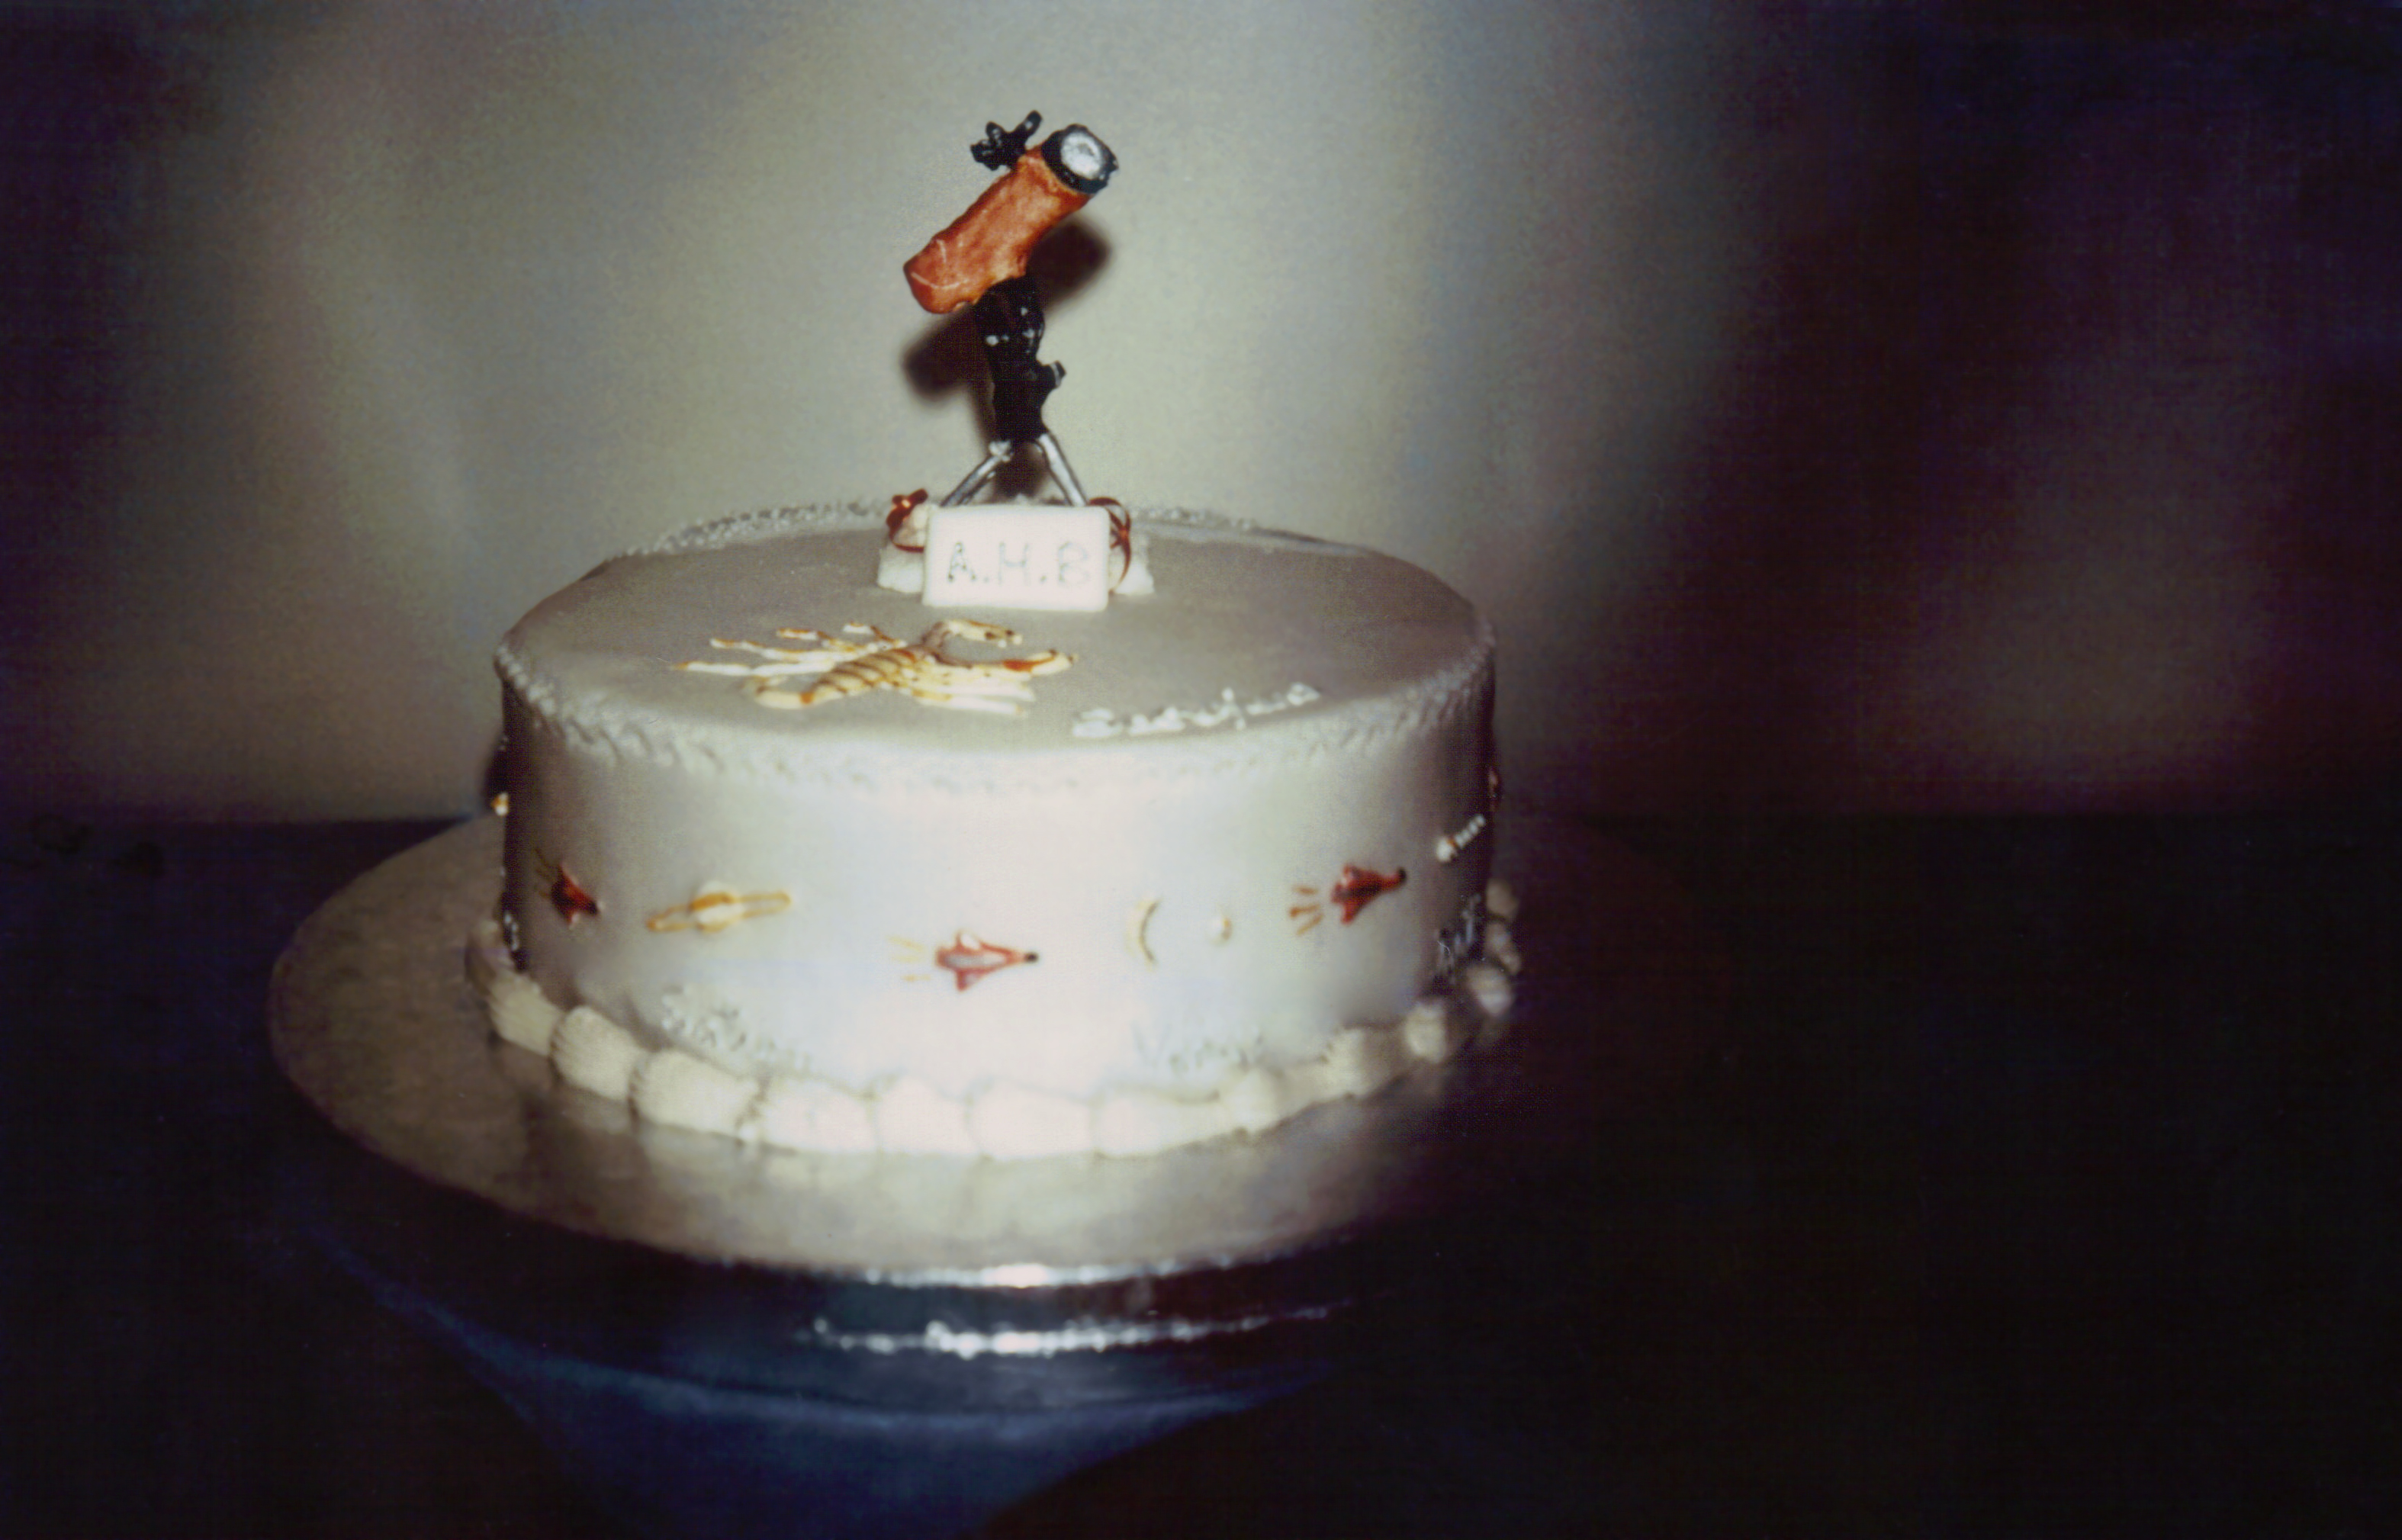
\includegraphics[width=0.9\textwidth]{photos/cake-astronomy.jpg}
  \caption{Tony's 60th birthday cake had an astronomy theme.}
  \label{cake-astronomy}
\end{figure}

I spend the whole of one day fashioning a telescope which was a
nightmare as the wretched thing kept falling over! However, it was OK
on the day and Tony was surprised and delighted. Crikey! I held my
breath!

We had to find somewhere to live and chose a location close to Phil
and Enid Hardisty -- Lombardy East -- the house was in need of repair
and I would be collected from our temporary home in a suburb of
Johannesburg by the man and his son who were to repair the house. I
was complete with bucket, mop, and apron, etc. and set about making it
more habitable.

One day he took a wrong turning and we found ourselves in Alexandra
township -- very, very black and awful. But there must have been
something of Nigeria left in me because I felt I had come home and
said ``this is more like it''! Both men thought I had gone mad!

We settled down to life in Johannesburg, South Africa. Elizabeth came
back to us from her English boarding school and went to Roedean. Where
she did well and obtained a good matric. Richard went to St. John's
college as a weekly boarder. He seemed very upset when we took him
back on Sunday evenings but he has said that he absolutely adored
being there. Just shows how one can get the wrong impression! Richard
also won his matric and settled down to a career in the hotel industry
and training first of all with Holiday Inn.

We had settled in the house in Lombardy East when we learned that the
house was to be auctioned to pay for debts incurred by the previous
owners. We protested of course. But, after much unpleasantness, we
moved to a flat in Corlett Drive which was lovely but had the
disadvantage of facing west and, in the Johannesburg summer, it was
not an ideal place to live.

%% Removed to reduce duplication in next paragraph:
% ; we finally found our ``resting place'', a
% house in Bryanston owned by the company and about to be vacated by an
% employee and his family who were returning to Australia. We acquired
% the house for a song and we also acquired a most wonderful dog. An
% alsatian (German Shepherd) for he had belonged to this family and they
% wanted to leave him behind -- so long as we promised to take good care
% of him.

Having been unlucky with the house and flat we first lived in in
Johannesburg we were pleased to find another house in Bryanston. It
was offered to us to buy at a low price (by the company, Barlow's) as
the occupants were leaving for Australia; they offered us their dog
after making sure we would give him a good home and we were to have
ten years of pleasure from this wonderful animal -- an intelligent,
handsome, and faithful german shepherd (see Picture~\ref{sherman}). I
was often alone all day and he would station himself outside the room
I was working in so that he was always on guard. Elizabeth trained him
well in obedience.

\begin{figure}
  \centering
  \begin{tabular}{cc}
    \subfloat[Sherman.]{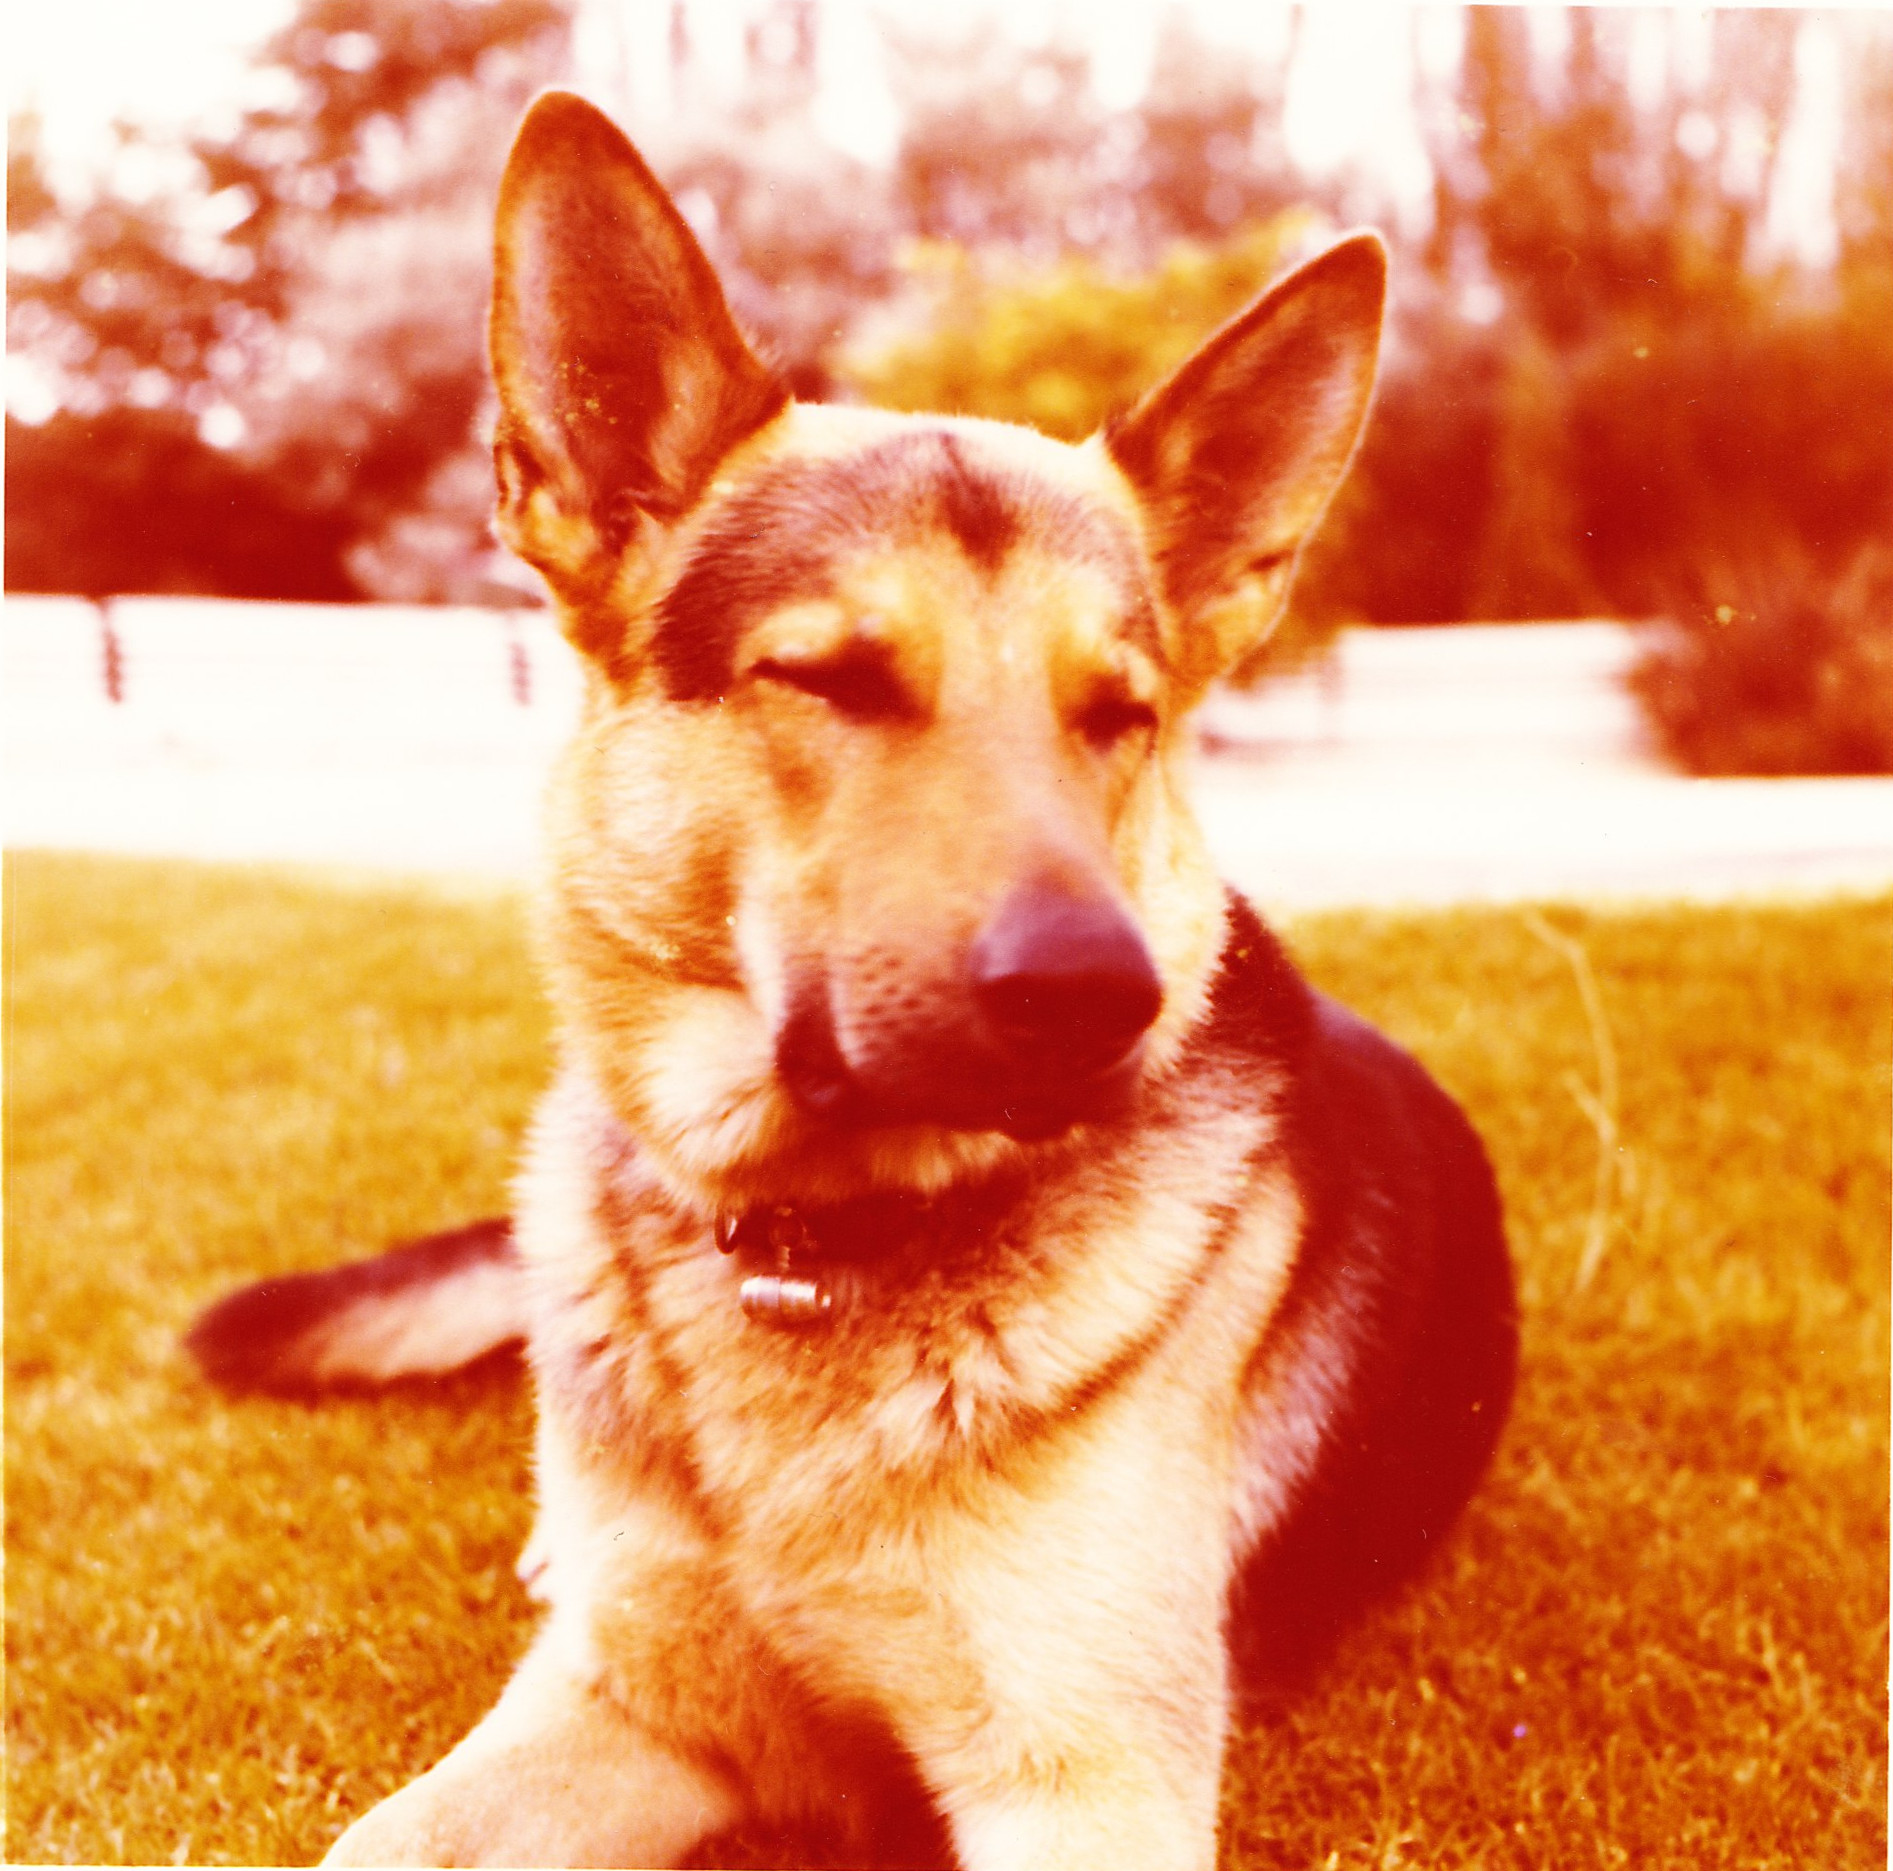
\includegraphics[width=0.45\textwidth]{photos/sherman.jpg}\label{sherman}}
    &
    \subfloat[Sydney.]{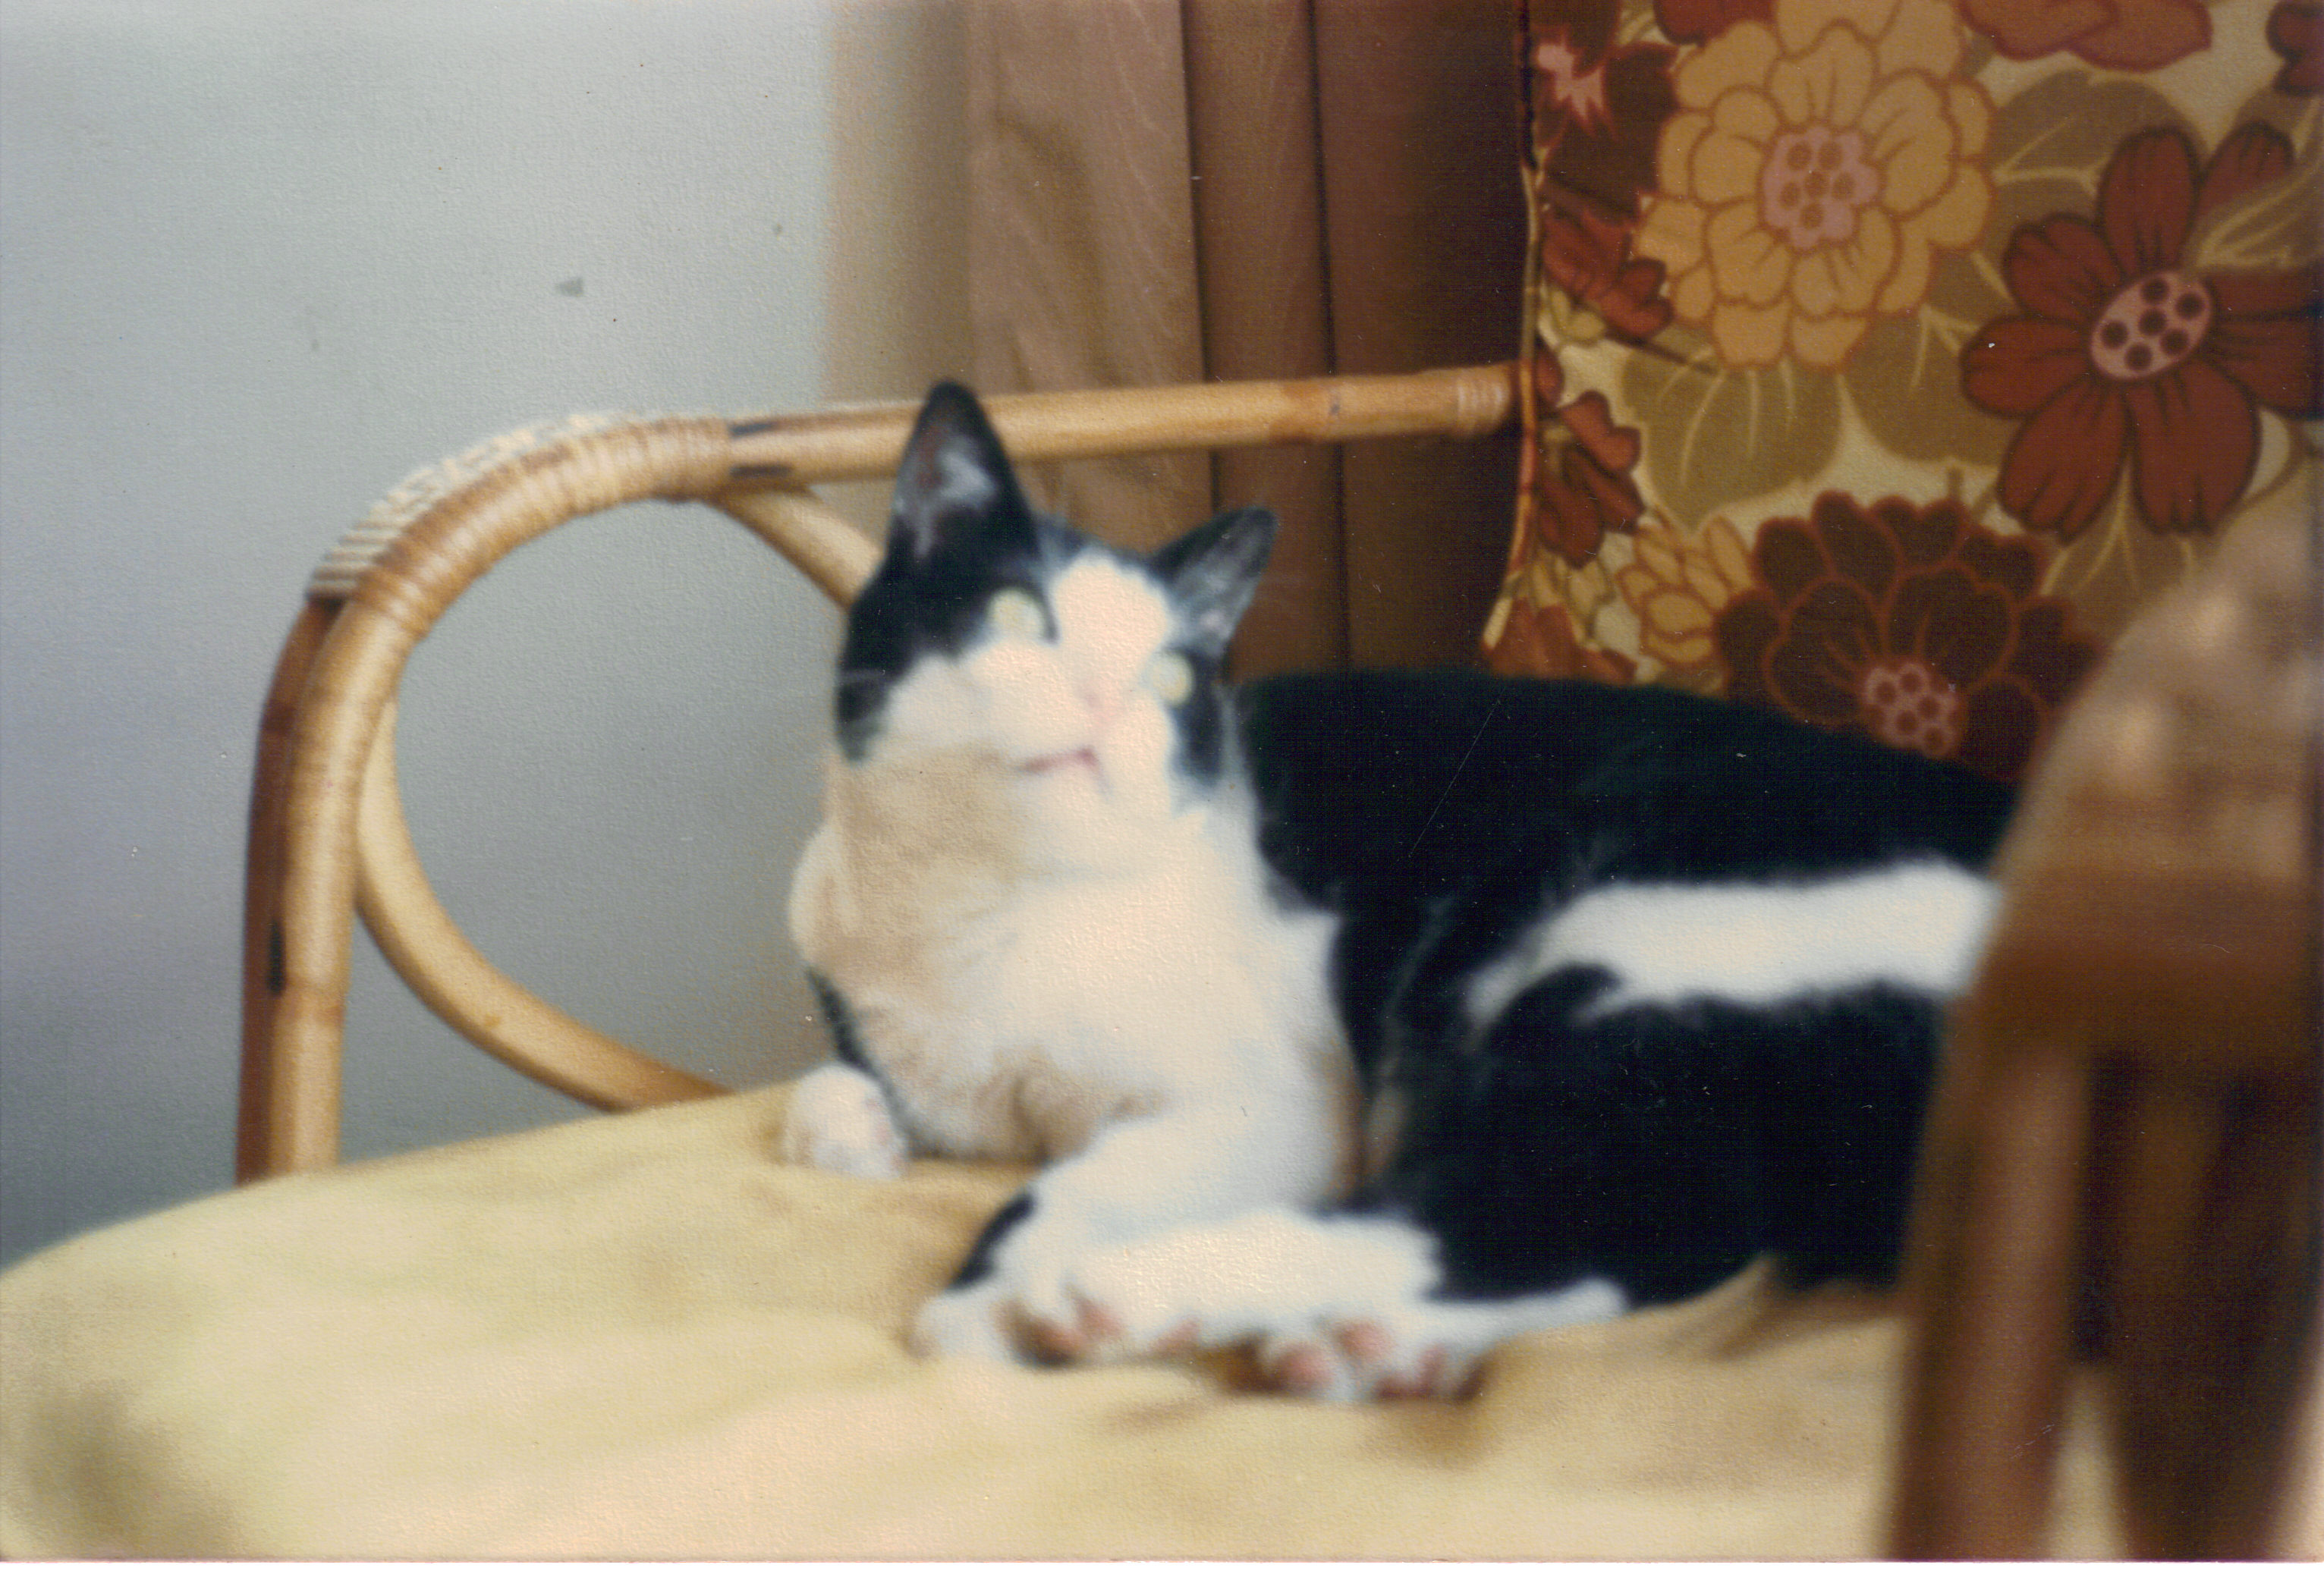
\includegraphics[width=0.45\textwidth]{photos/sydney.jpg}\label{sydney}}
    \\
  \end{tabular}
  \caption{Pets.}
\end{figure}

% \begin{figure}
%   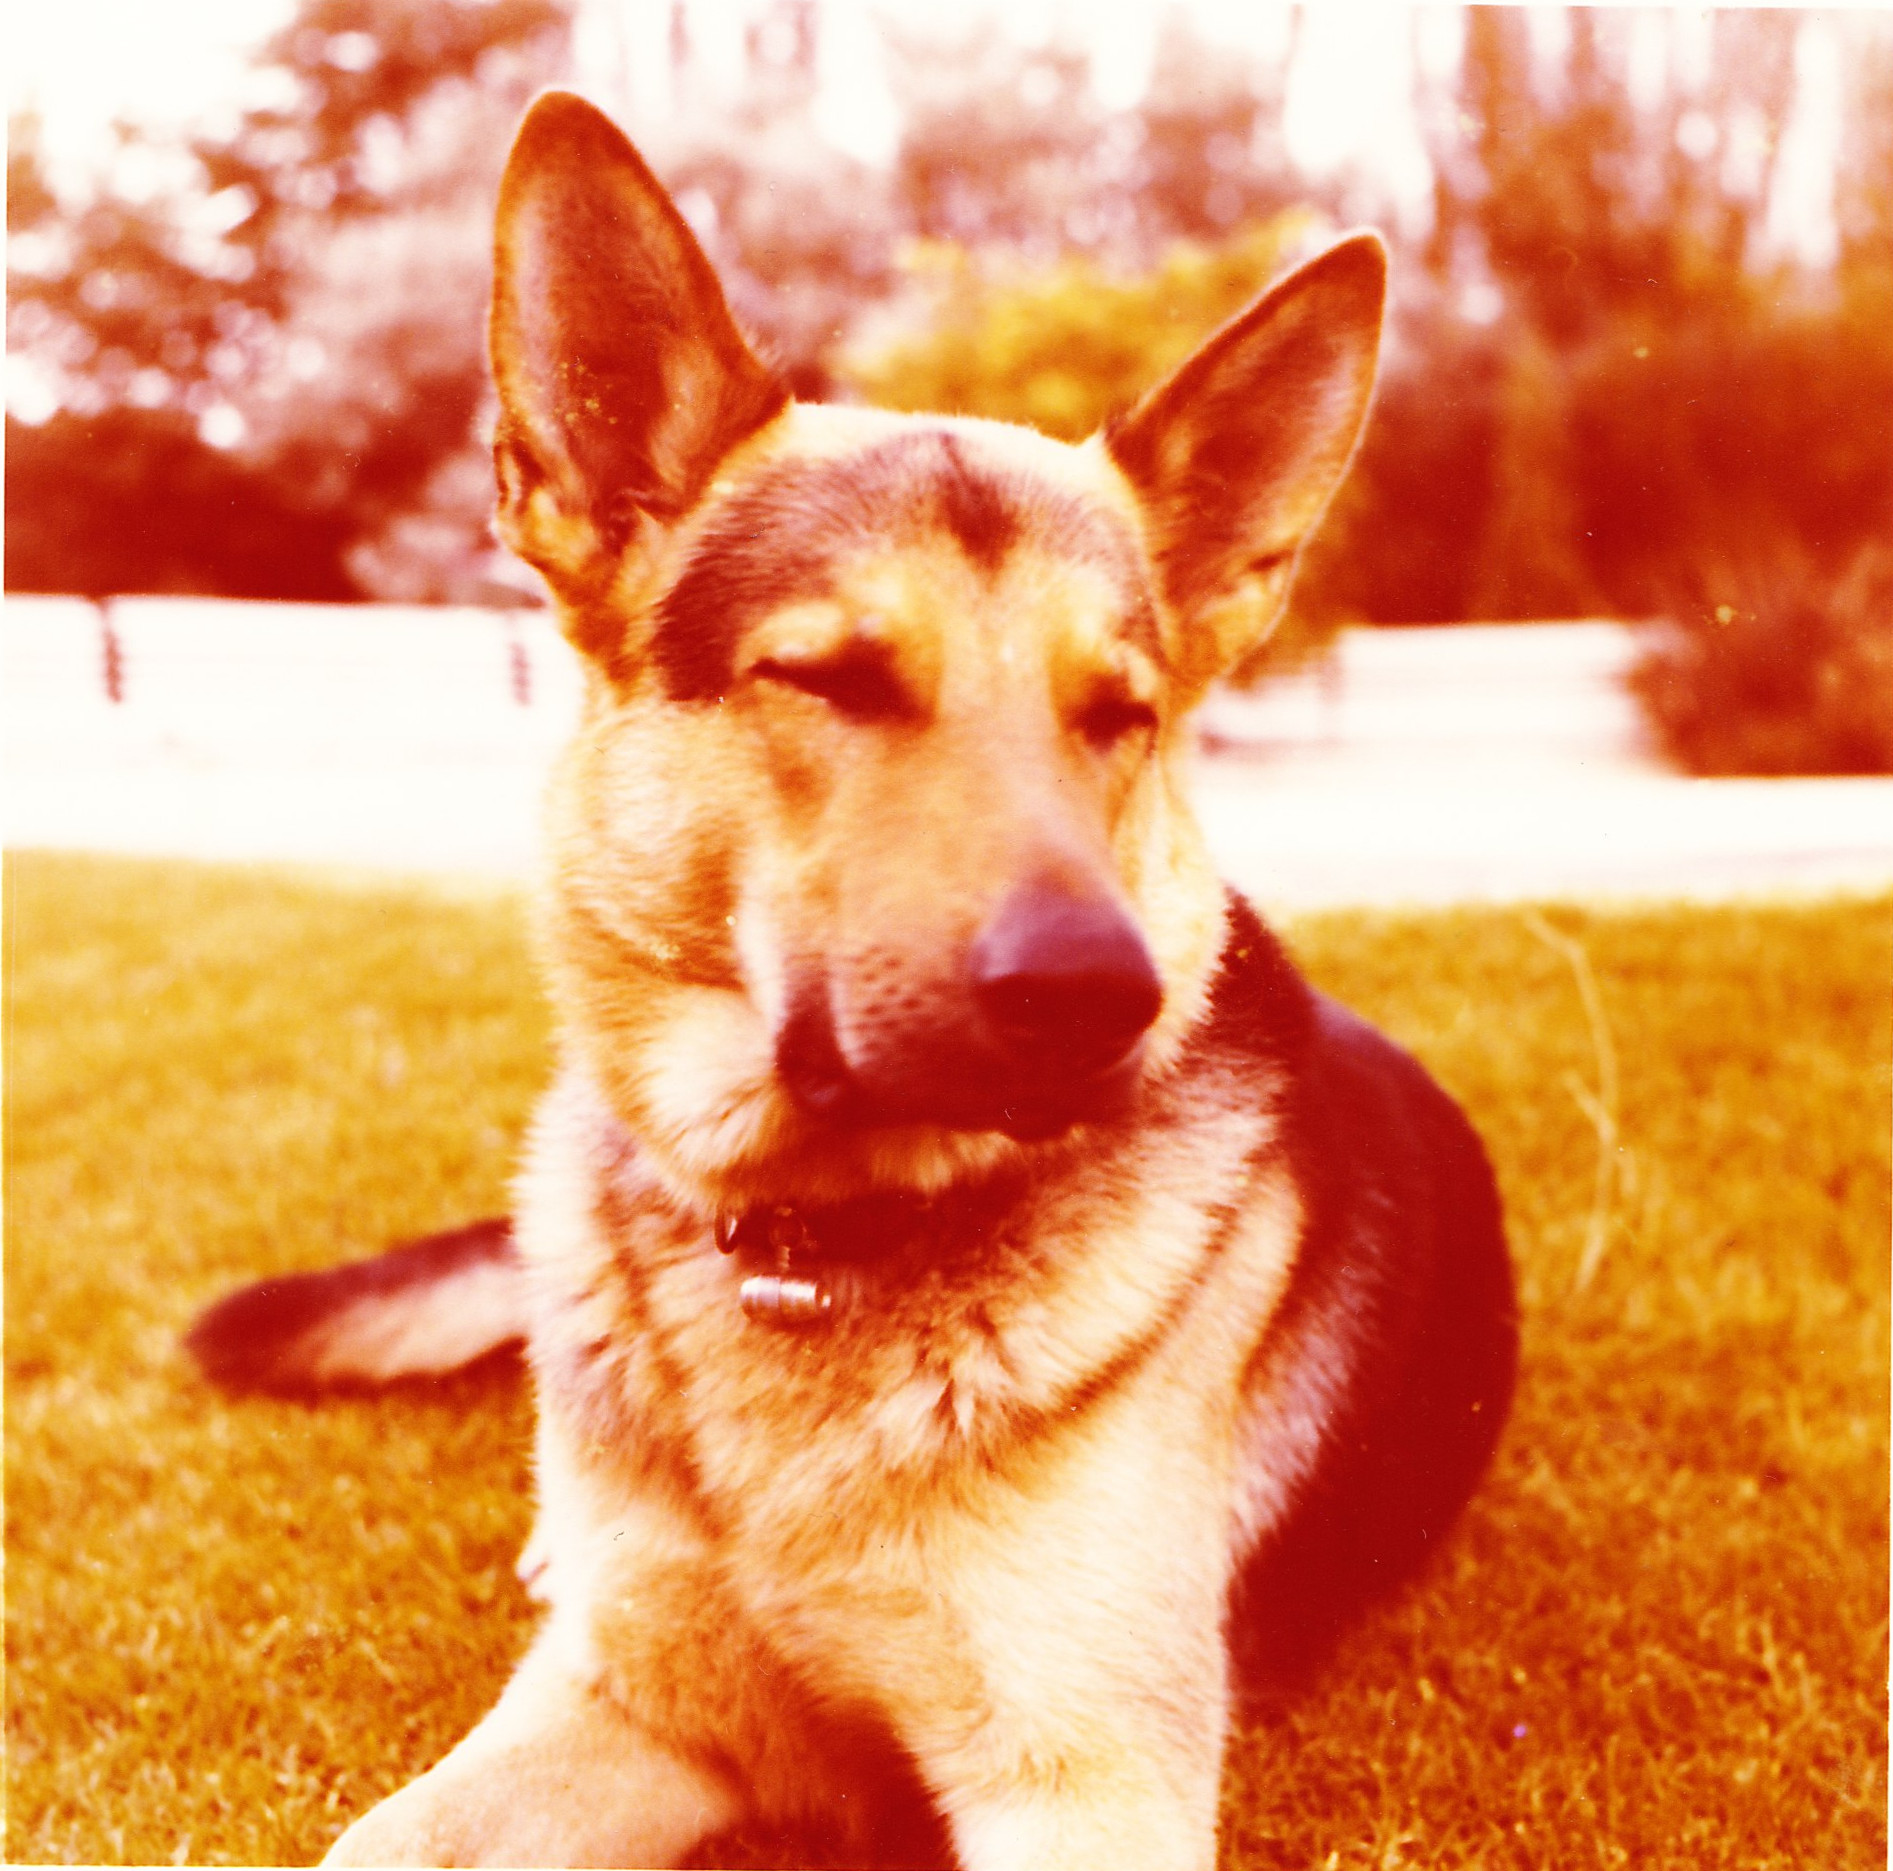
\includegraphics[width=\textwidth]{photos/sherman}
%   \caption{Sherman.}
%   \label{sherman}
% \end{figure}

% \begin{figure}
%   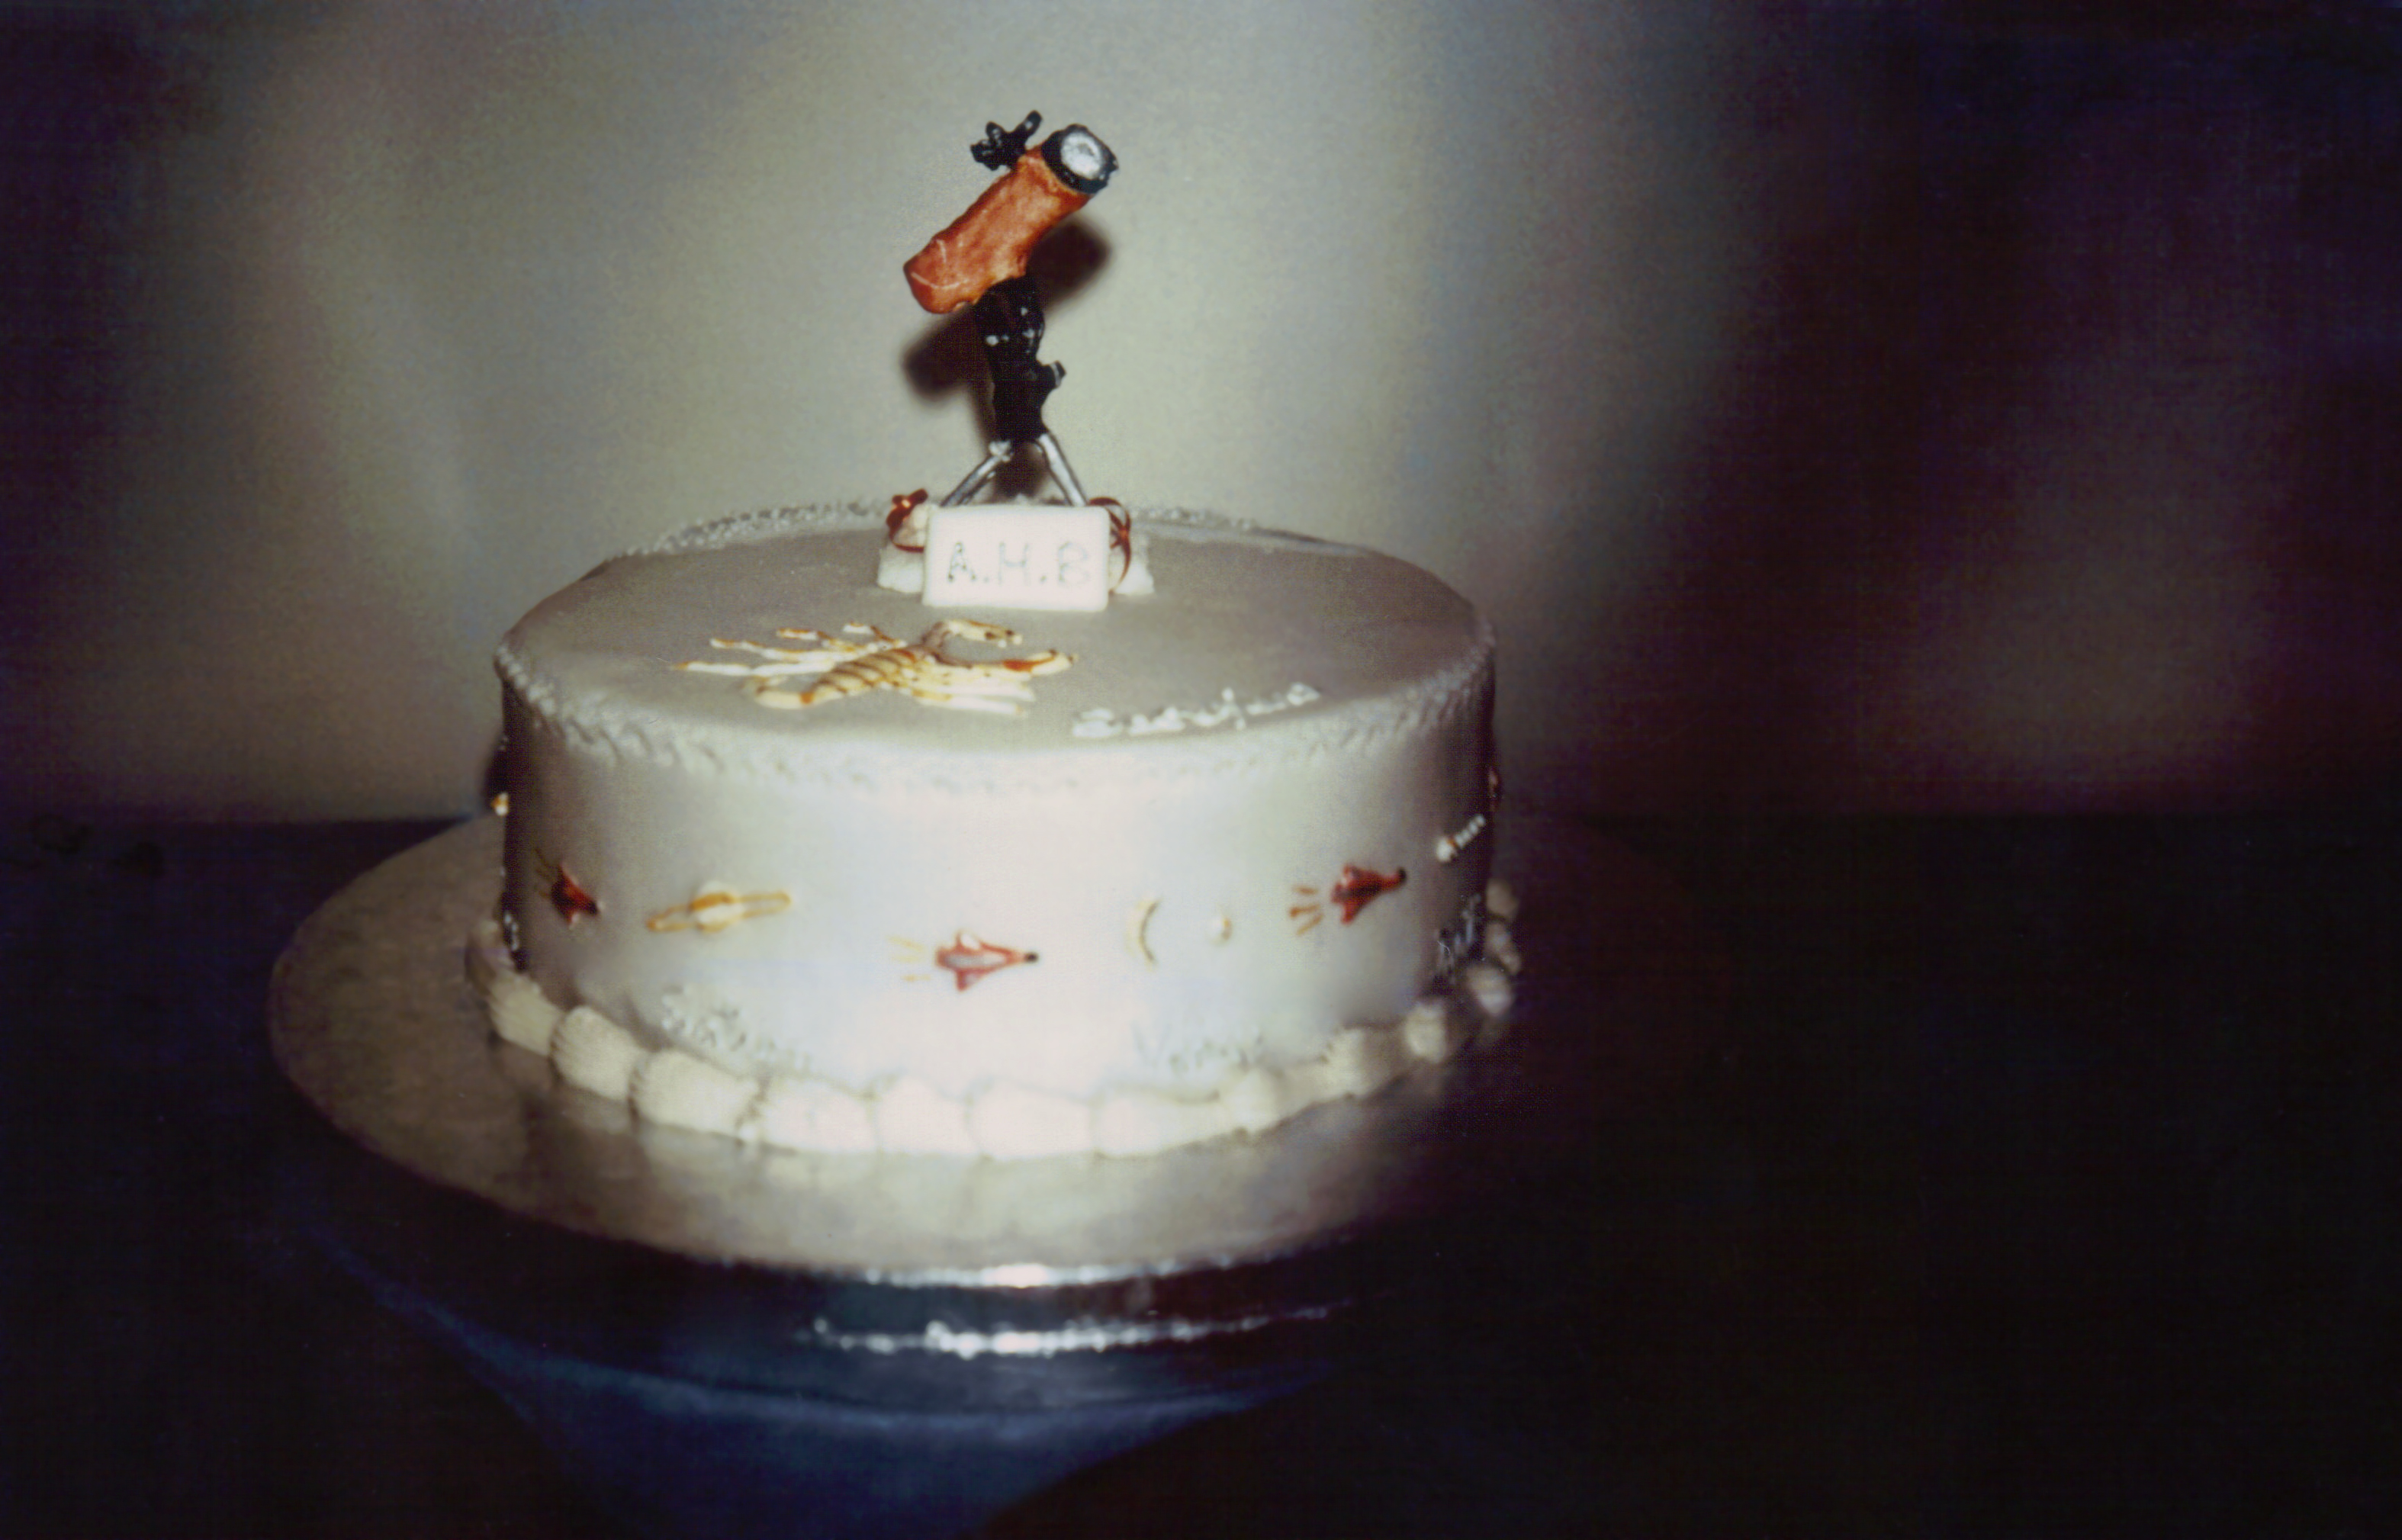
\includegraphics[width=\textwidth]{photos/cake-astronomy}
%   \caption{Tony's 60th birthday cake had an astronomy theme.}
%   \label{cake-astronomy}
% \end{figure}


We acquired another animal during our stay in Bryanston -- this time a
kitten Elizabeth had found and adopted whilst she was in residence at
the hospital. He was not allowed to stay there so we took him to live
with us. He was another handsome specimen and he grew into an enormous
cat - black with white ``socks'' and white ``bib''. He was called
Sydney (see Picture~\ref{sydney}). We feared for Sydney's life if he
came up against Sherman and tried to keep them apart but they met in
the gardens and took to each other. The cat was the tormentor and
would jump out at Sherman from behind a tree, but they were only
having some fun. Sydney did not like me and would leave a room if I
entered -- often leaving the comfort he found on Tony's lap -- his
favourite place. I often wondered how I had offended him!

% \begin{figure}
%   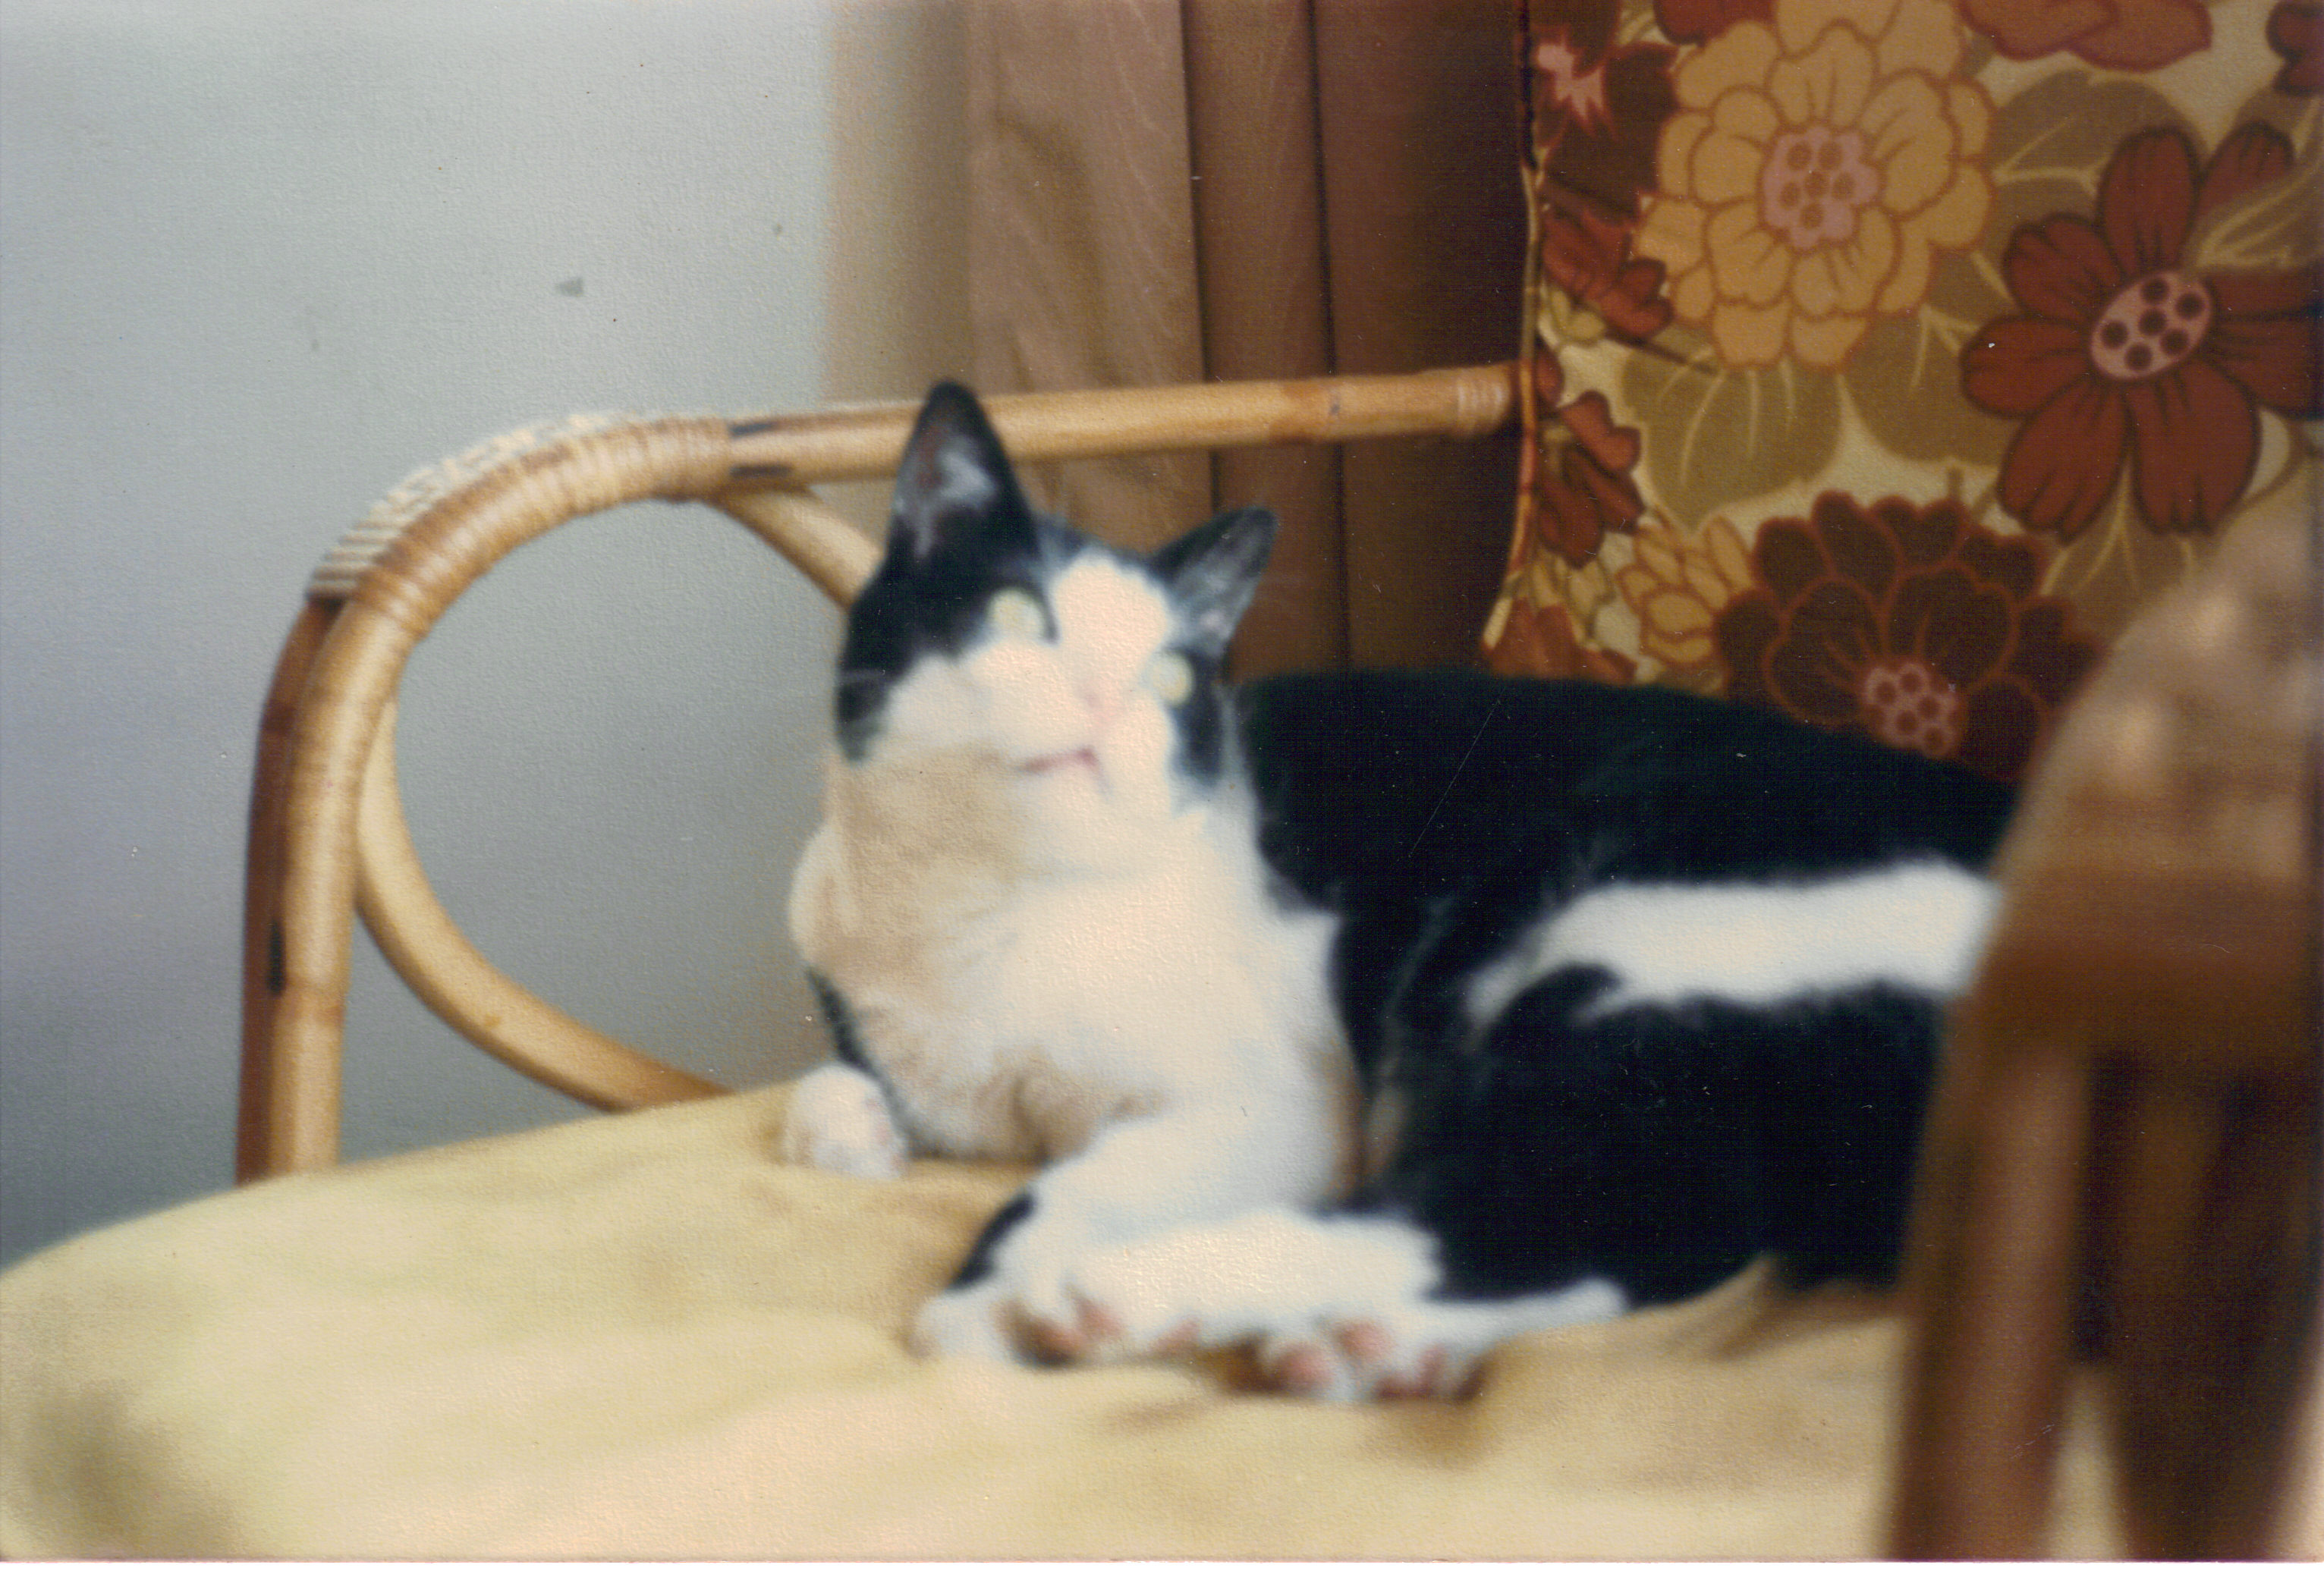
\includegraphics[width=\textwidth]{photos/sydney}
%   \caption{Sydney.}
%   \label{sydney}
% \end{figure}

Sadly both animals suffered illness and had to be put down; Sherman
was twelve and Sydney sixteen. We loved them so much that we cried
like babies and could not contemplate ever having another pet --
although somewhere along the way Elizabeth acquired a budgie.

Another joy about living in Bryanston was that Tony gave me a tennis
court (with lights) -- a most generous present. If people came in the
evenings we would play under the lights (no shadow). My tennis party
took place on Tuesday mornings: six to eight of us having a wonderful
time under a big tree with (naturally) refreshments and chatter (see
Pictures~\ref{tennis}). Looking back it was a superb time of life for
me.

\begin{figure}
  \centering
  \begin{tabular}{c}
    \subfloat{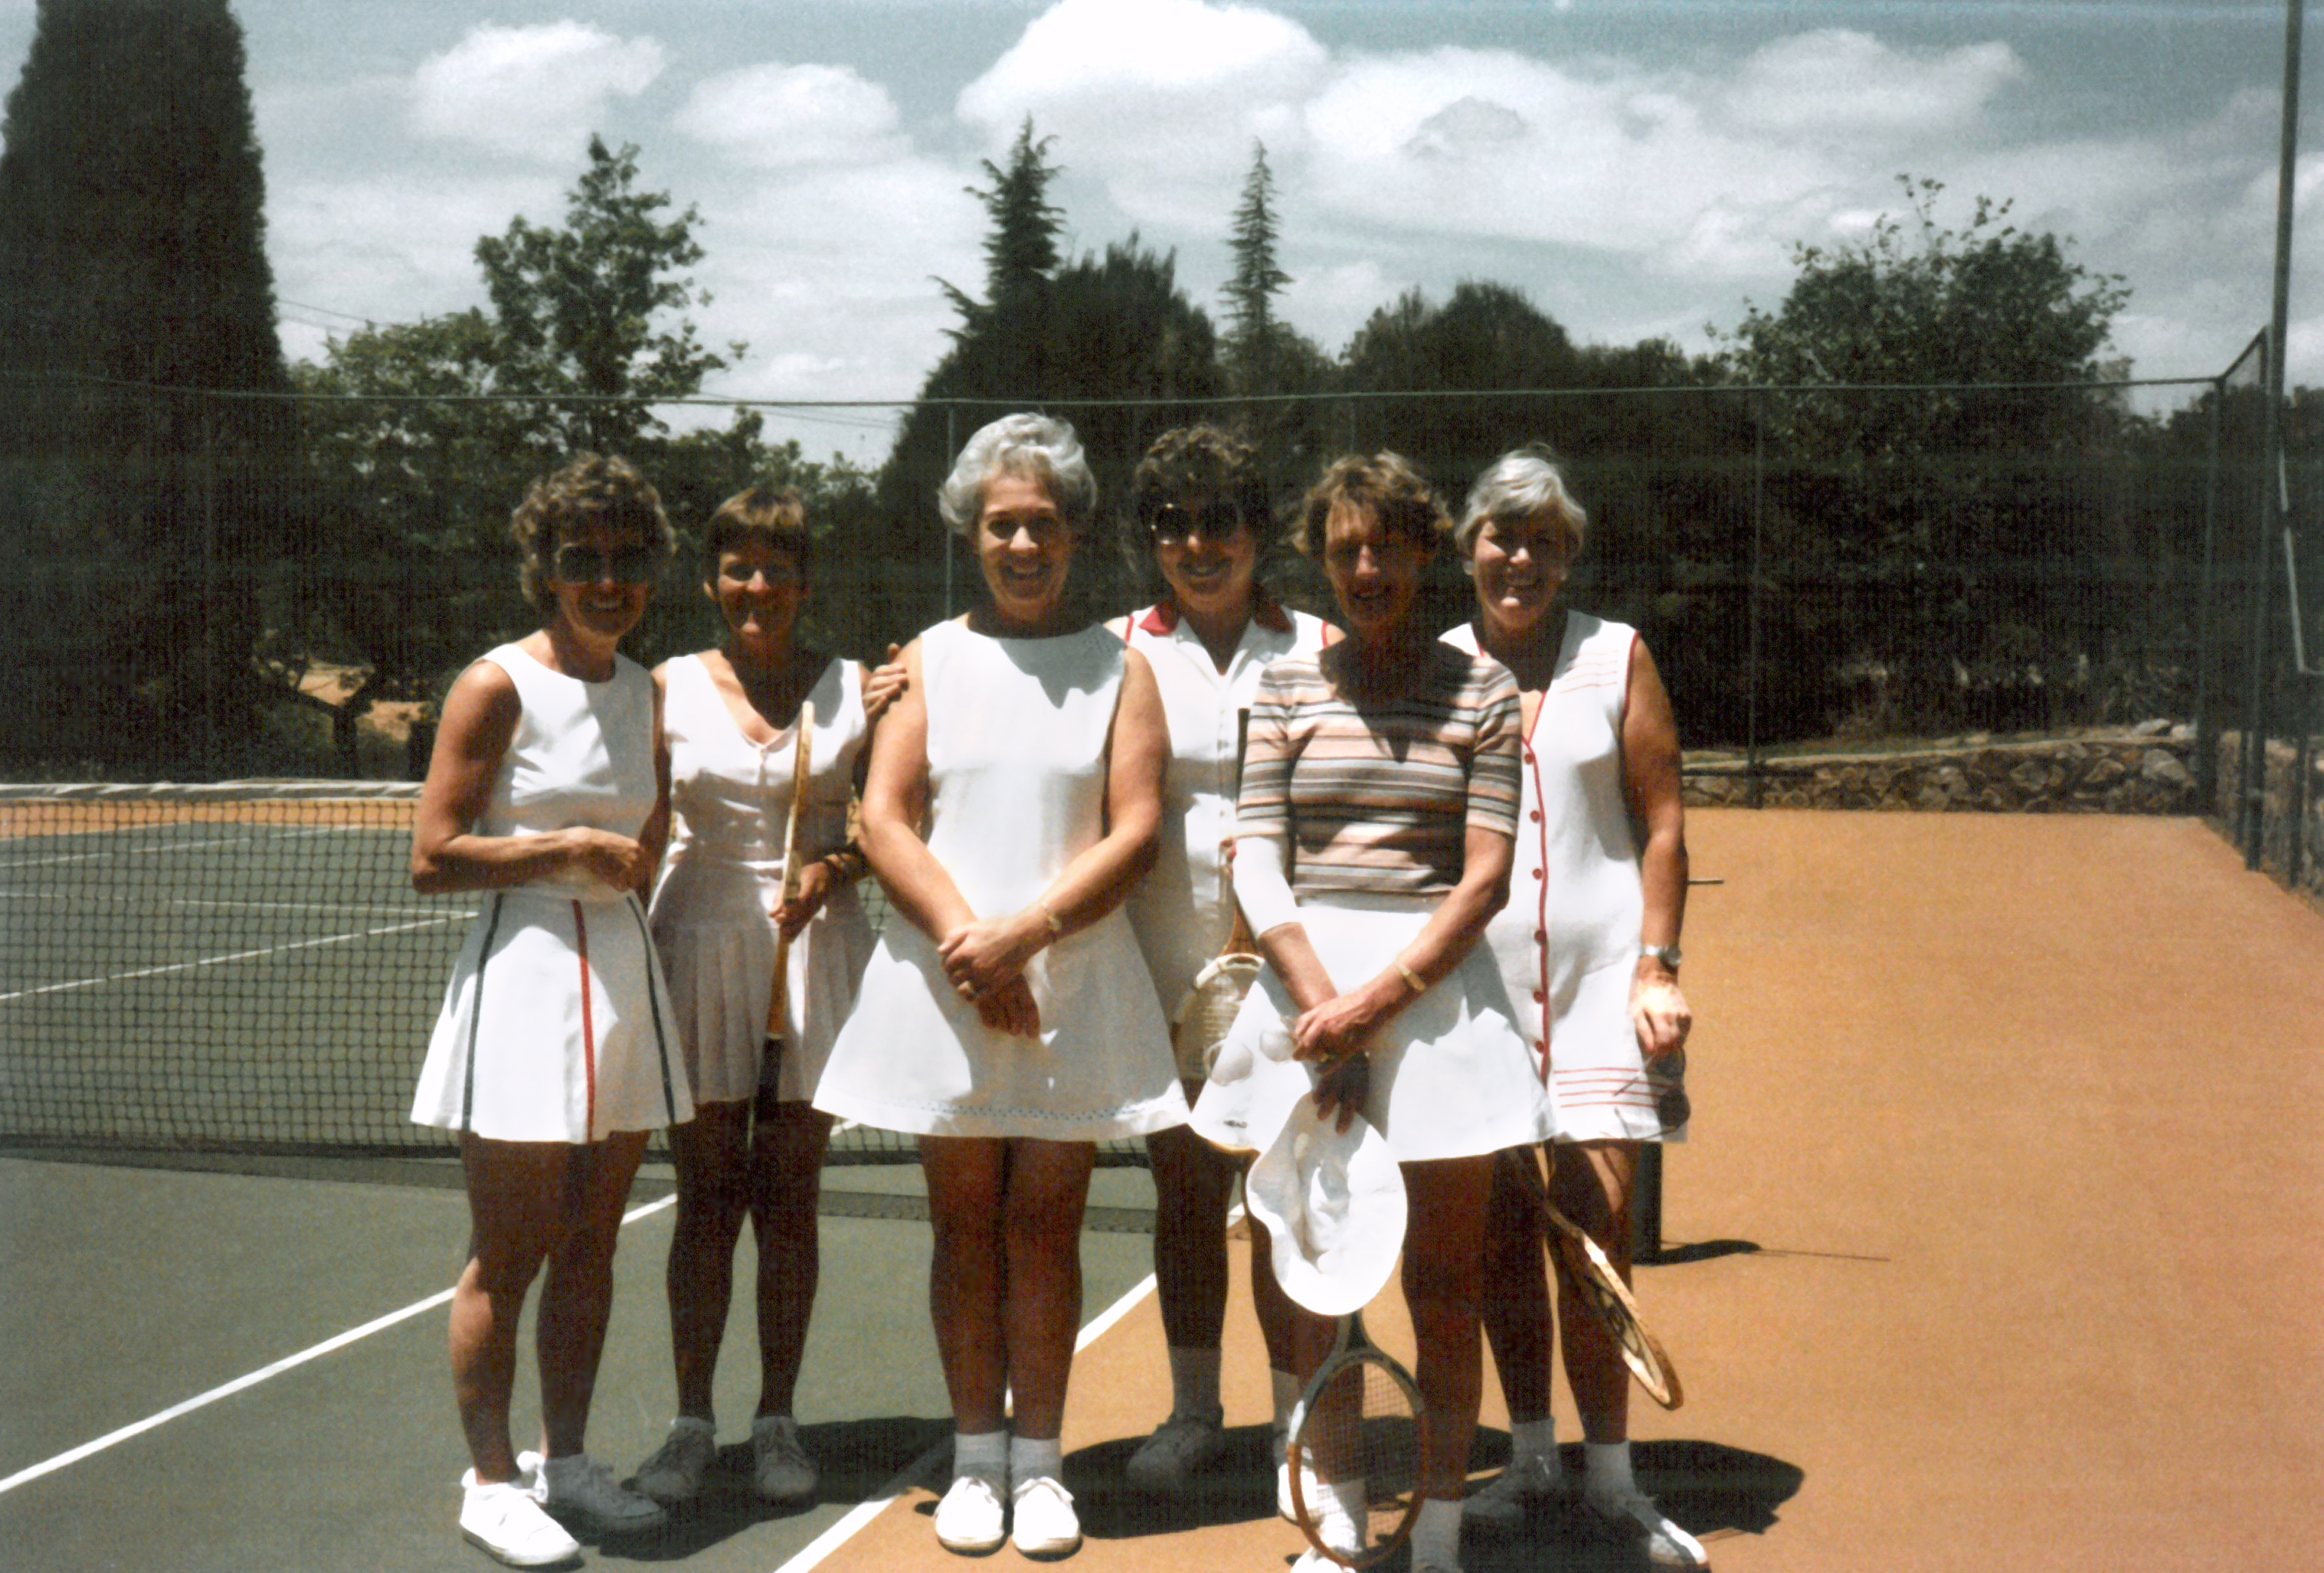
\includegraphics[width=0.9\textwidth]{photos/tennis-group.jpg}\label{tennis-group}}
    \\
    \subfloat{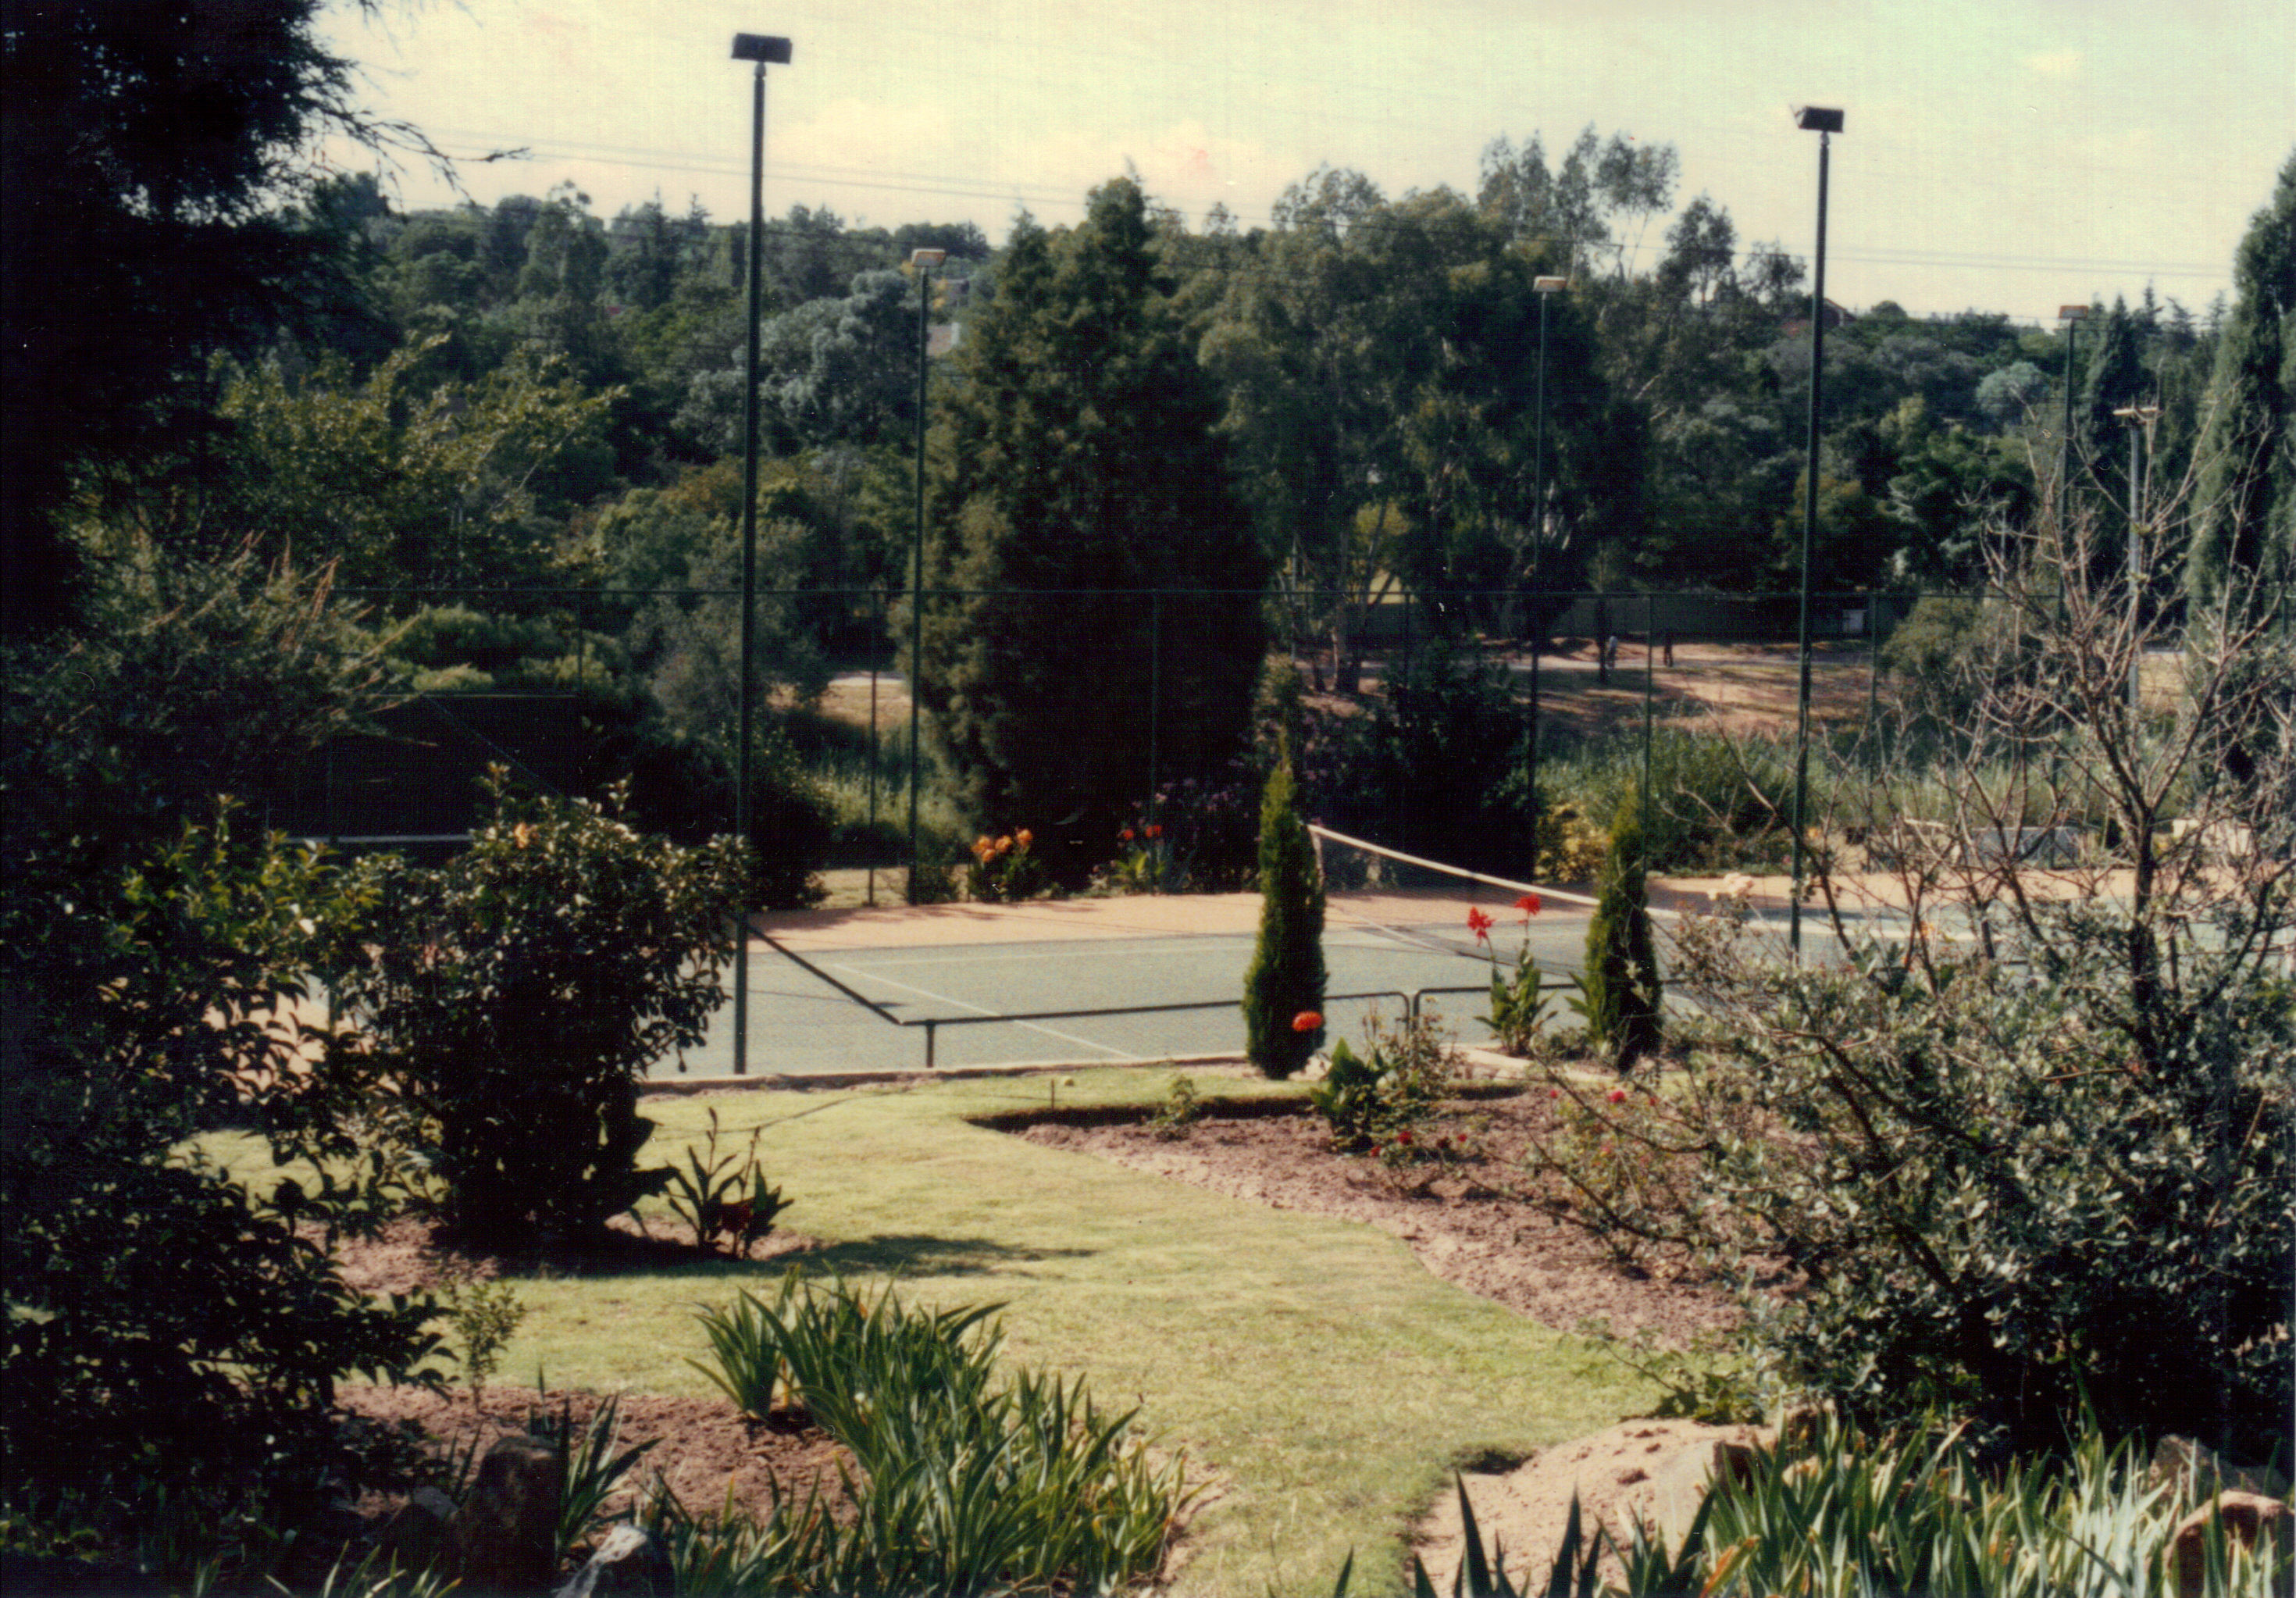
\includegraphics[width=0.9\textwidth]{photos/tennis-court.jpg}\label{tennis-court}}
    \\
  \end{tabular}
  \caption{Madge's tennis group and tennis court.}
  \label{tennis}
\end{figure}

% \begin{figure}
%   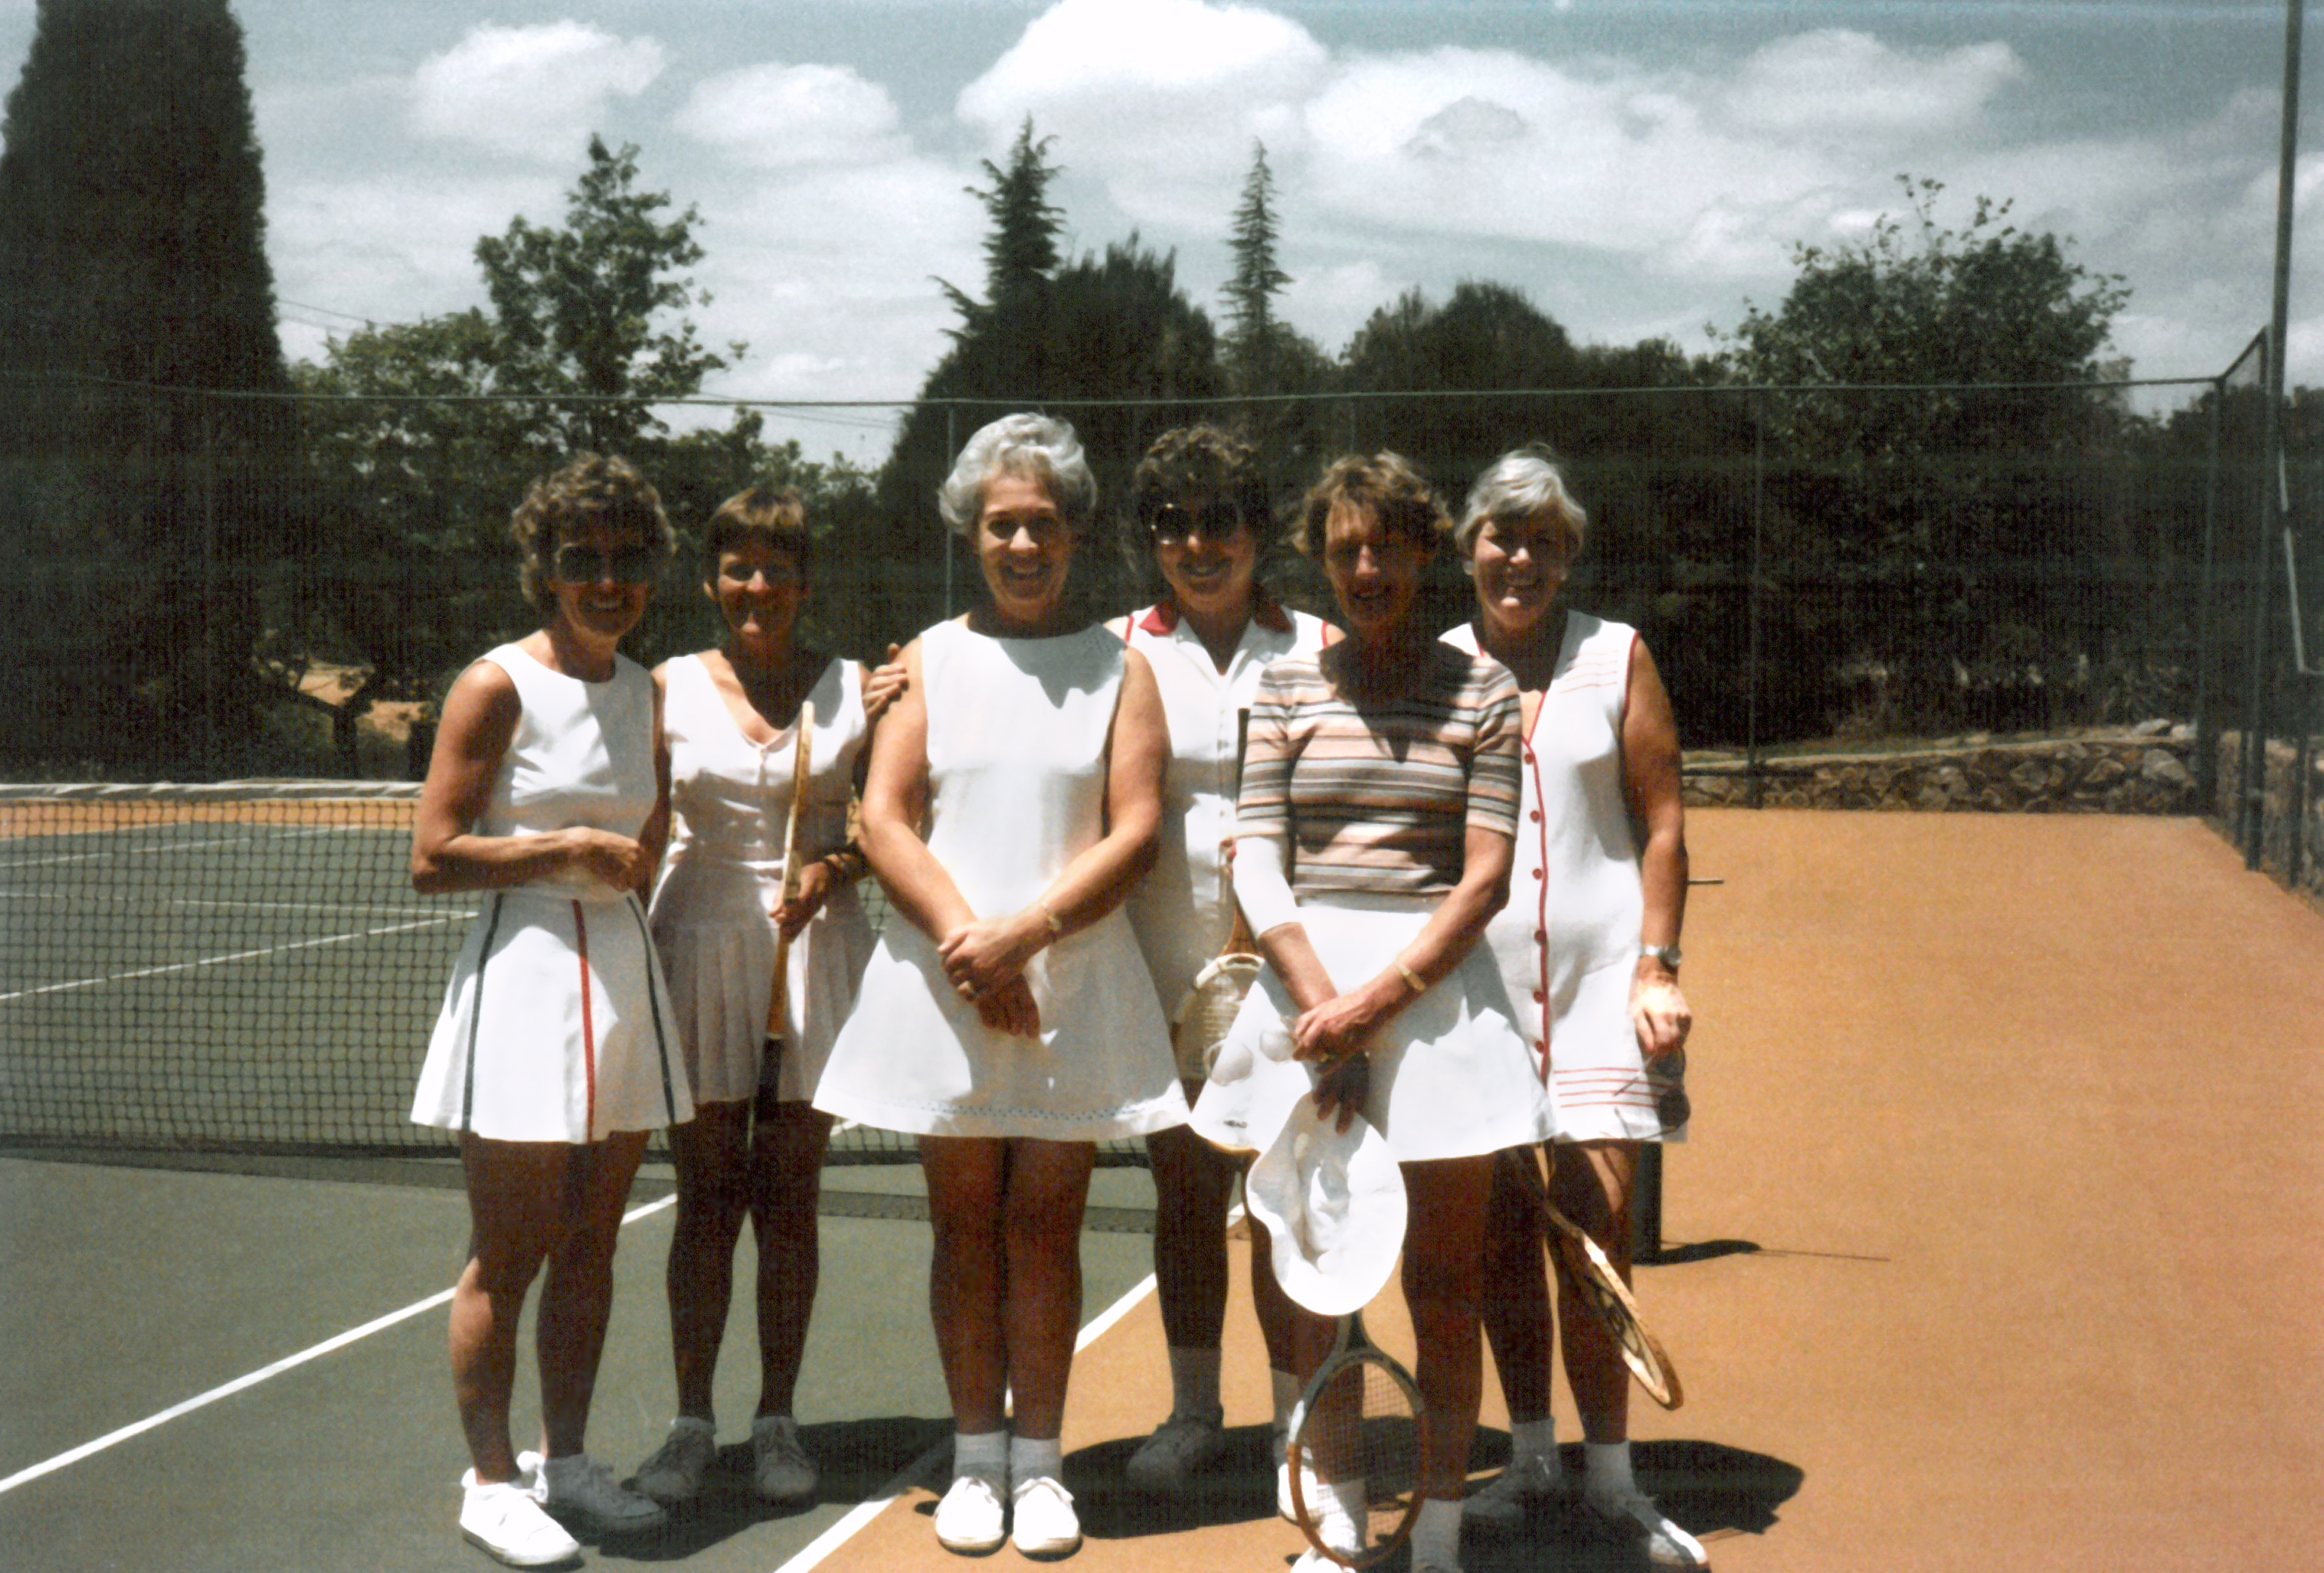
\includegraphics[width=\textwidth]{photos/tennis-group}
%   \caption{Madge with her tennis group (Johannesburg, 19??).}
%   \label{tennis}
% \end{figure}

% \begin{figure}
%   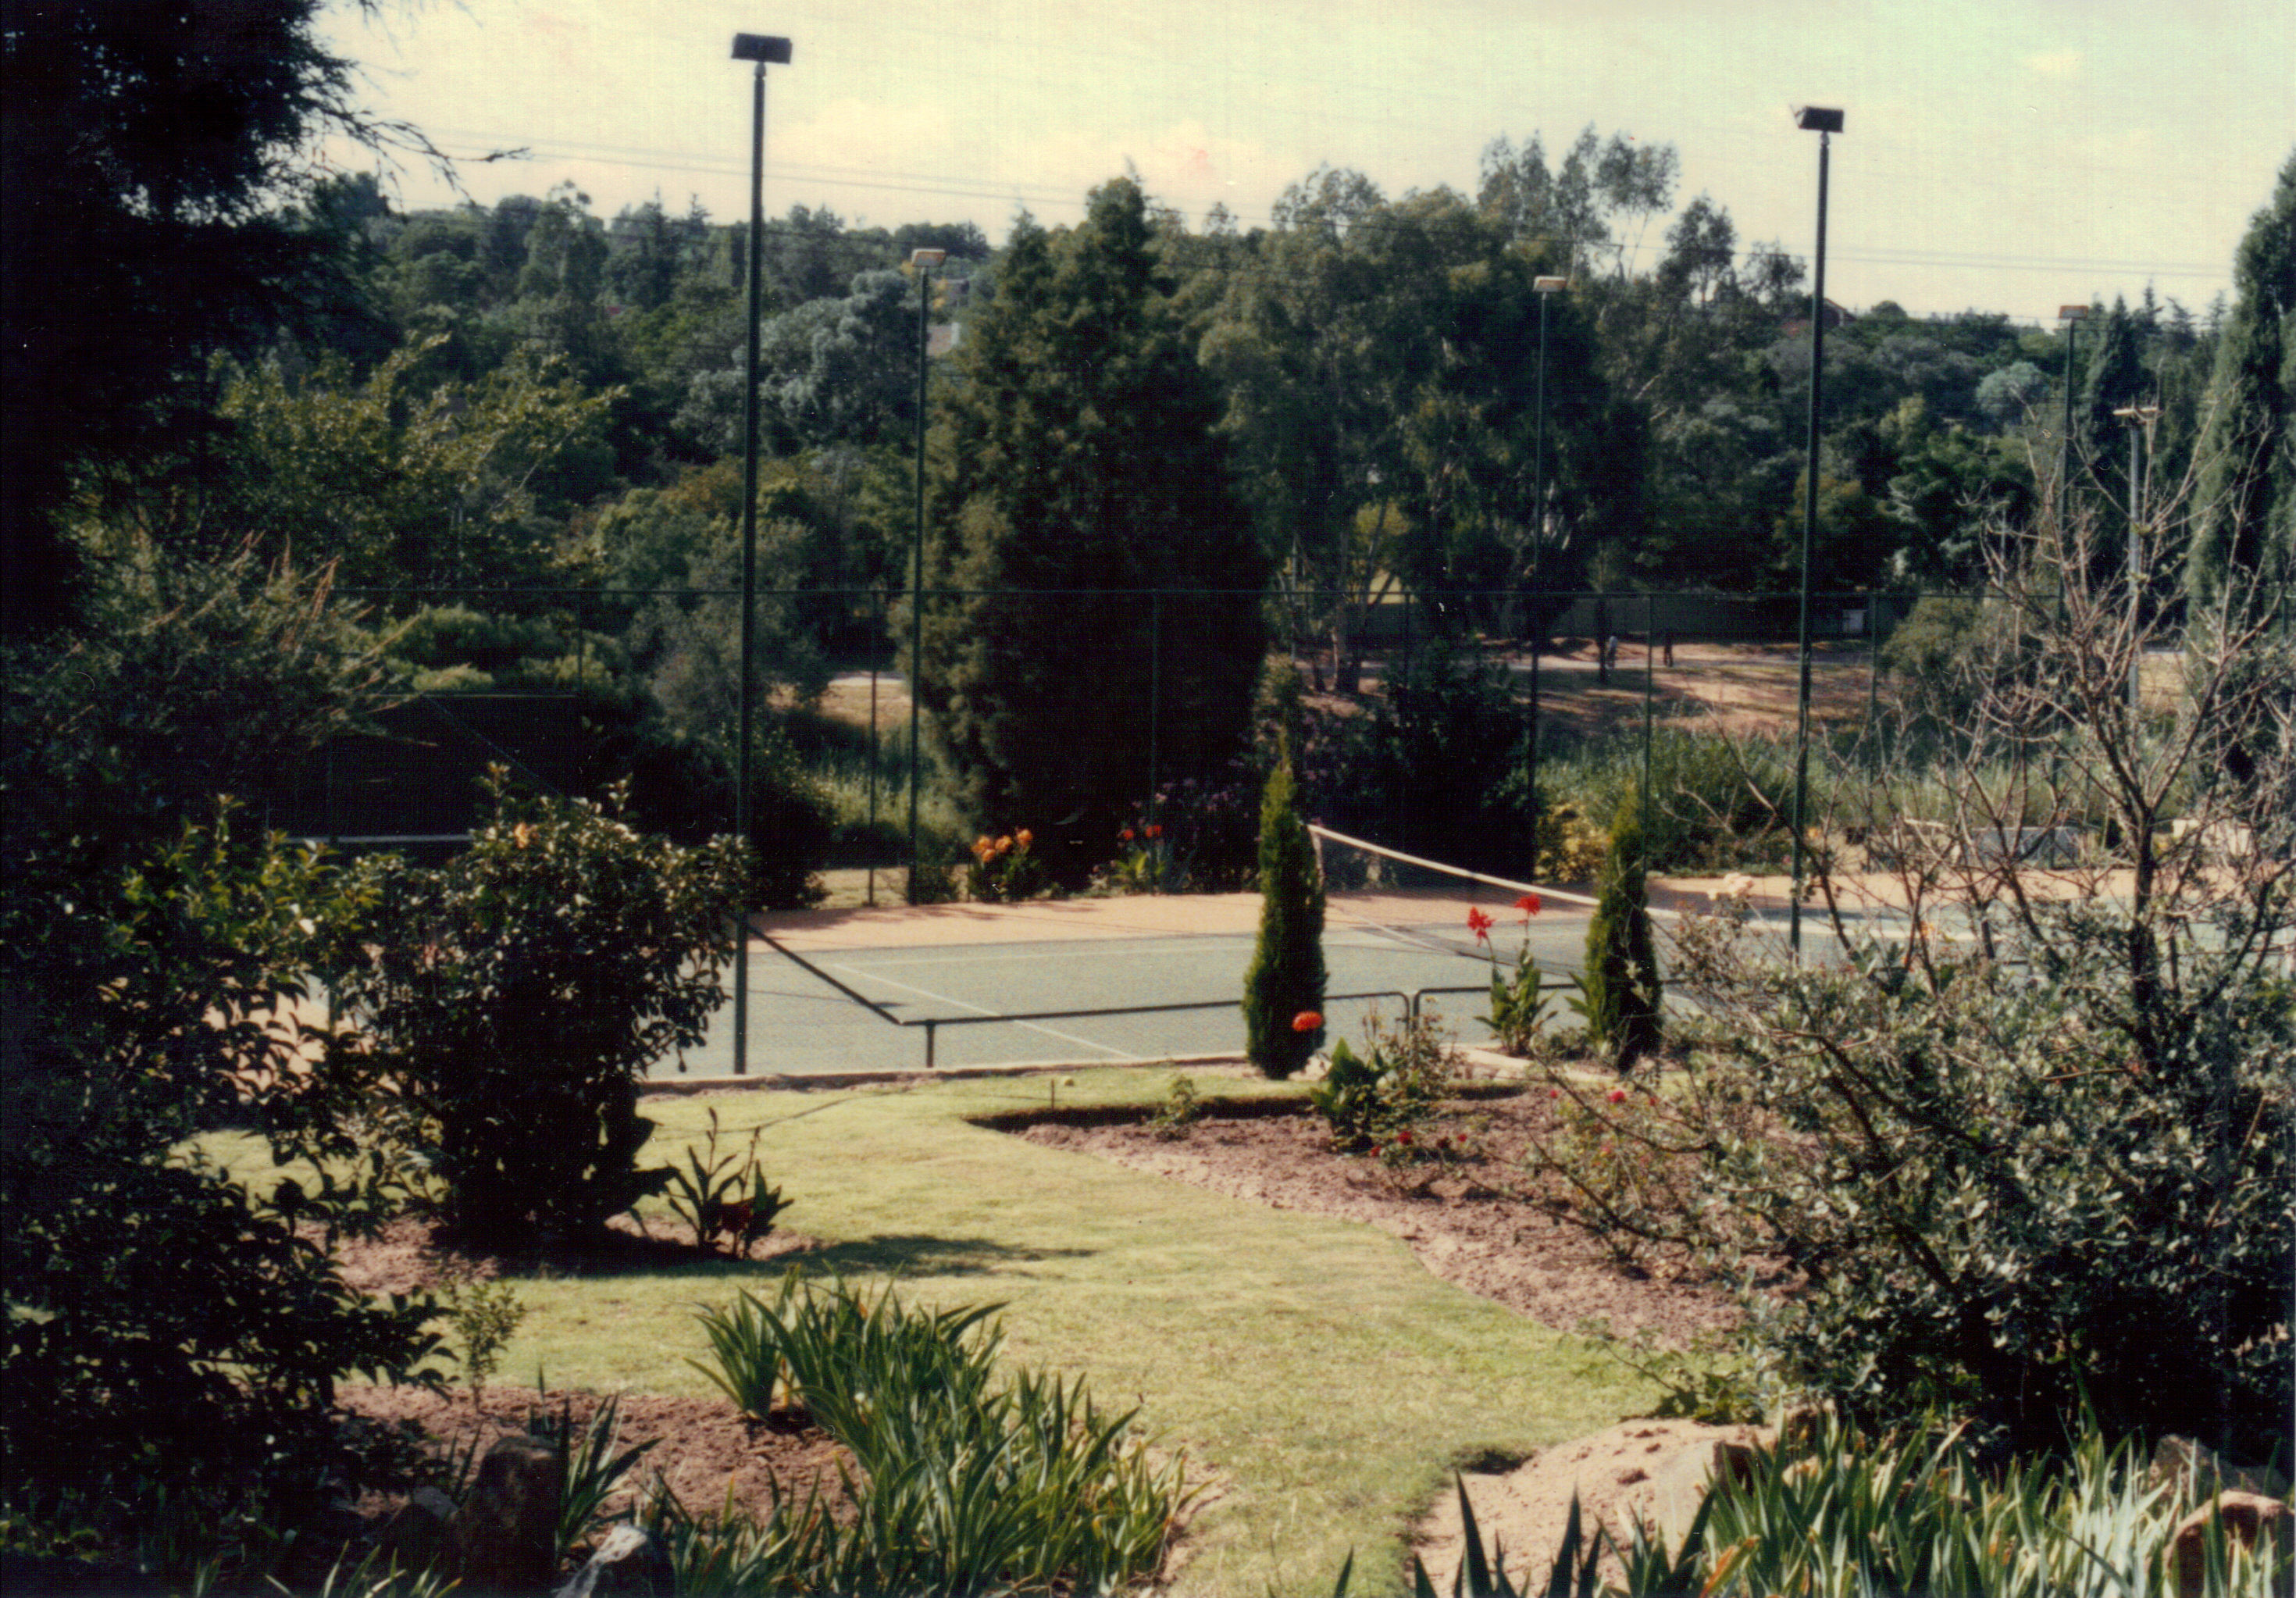
\includegraphics[width=\textwidth]{photos/tennis-court}
%   \caption{Madge's tennis court.}
%   \label{tennis-court}
% \end{figure}

At this time Elizabeth was at school at Roedean (we did not know then
that she was not happy there but she did very well anyway). Richard
went to St. John's college in Johannesburg and we had no idea that he
loved it! Being a weekly boarder, he had to be taken back to school on
Sunday evenings and got extremely upset about being left but,
apparently, pulled himself together very quickly. Little devil!

Sherman had a lovely nature -- but \textit{could} be nasty if
necessary and he became a wonderful friend and companion to us all --
particularly to me as I spent much of the day alone. He joined us when
he was two and lived to fourteen. Sadly arthritis and a growth on the
liver caught up with him and he had to be put down.

A cat also came into our lives and he and Sherman became good friends.
The cat (kitten then) was really Elizabeth's but it became impossible
(and not allowed) for her to keep him in the hospital where she was
training in nursing (and achieved her B.Sc.) So we took him on and
loved him. He adored Tony but did not like me. If I entered a room he
would even jump off Tony's lap and leave the room -- even though I was
the one to give him his meals and try to stroke him. Sadly in his old
age he became ill -- and very fat and incontinent -- and we had to say
``goodbye'' to him too.

We never wanted another animal to replace these two who were
outstanding.


\chapter{Israel}

Whilst working for the GEC in Nigeria, Tony had business dealings with
an Israeli company and, on one of his visits to Israel, he took me
along. Being in the Middle East, there were strong resemblances to
Turkey and I felt really at home.\footnote{This was a 12~day trip in
  1984. Elizabeth was married and had just had Andrew. Richard was 20
  and embarked on his hotel training.}

Tony hired a guide for us whose name was Teddy Vardi and we were so
lucky to be looked after by him. He seemed to know every inch of the
country and Israel came alive to me. It was magic to me to go to
places where Christ had walked; I was swept away by Jerusalem.
Learning what had happened there and the history etc. was
mind-blowing.

In Teddy's car we covered so much of the country and he described
everything so well. We saw many places: Tel Aviv, Tiberias, Hebron,
and etc. I had to write down all we had seen every evening; it would
have been impossible to remember it all.\footnote{I wrote a journal
  which accompanies these notes -- see Appendix~\ref{Israel}.} I
remember so well going to Masada, passing by Jericho and the Dead
Sea. Masada is the place where so many Jews were massacred under
Herod's instructions. There must have been survivors for the story has
been told.

Another story, of course, is the massacre of the 6 million Jews by the
Germans before the outbreak of the second world war. It was
heartbreaking to visit the Yad Vashem, which is a monument to the Jews
who perished in the holocaust. A flame is kept permanently burning in
memory of those who perished. My memories are so clear about his
country and certain occasions do stand out -- the Friday evening
dinner with Gurion and Sara Meltzer (in Tel Aviv) when we were the
only gentiles. It was such an honour to be there.

It is altogether different to read about a place and then to visit it
and try to absorb the religious and historical aspects of it. My walk
up the Via Dolorosa where Jesus had carried his cross to the place
where he was to be crucified was unforgettable.

Goodbye to Israel. What a host of memories.


\chapter{Retirement}

Tony enjoyed his managing directorship but arrived at the moment when
he decided, at age 63, that he would like to take early retirement.

He had been quietly studying his beloved physics and astronomy as he
had done for many years and decided that now was the time to buy a
telescope. This was done through the Johannesburg planetarium and with
the help of Tom Geary and Wim Ahlers we found such joy and pleasure
from that wonderful instrument and Tony taught me so much about the
``heavenly bodies''. Really mind-boggling bits of information like --
``planet Earth could fit into planet Jupiter 1,000 times'' will always
stay with me.

After fourteen years in Johannesburg, we decided to move to Durban --
not only because Elizabeth and Matthew lived there, but also because
Natal offered a quieter and slower way of life. And so we found a
beautiful house (much too big for a retired couple, but we loved it)
in Winston Park, Gillitts. We had a super life there with much
entertaining. And, of course, the beloved telescope occupied much of
Tony's time and he started to enjoy inviting school children to come
and observe the skies. Our neighbour was a teacher and her garden was
used for ``viewings'', being less full of trees to block the
views. Oh! How those children loved those evenings, and the teachers
and parents who also turned up were fascinated by listening to Tony
pointing out stars and planets etc.; what a wealth of knowledge he had
and how he was appreciated.

When the Preston family left South Africa to emigrate to New Zealand
we were devastated and missed them terribly. But the time and
opportunities came for us to visit them and altogether we made four
trips, using a different airline each time. We were able to enjoy the
sights and delights of the different places we stopped at -- Hong
Kong, San Francisco, Sydney, Singapore, etc. I remember well the
cleanliness of Singapore and the beauty of the gardens with their
profusion of orchids -- and even the airport (once the Changi prison)
was decorated with orchids from end to end. In Singapore, also, we
went across to Sentosa Island to the museum where there are horrible
images of the Japanese occupation but also the triumph of the
Singapore people to regain their country and to make it so lovely
again.

In Singapore we had a memorable anniversary dinner at ``Raffles''.

New Zealand is a beautiful country and, on our first visit, we took
two weeks to explore the South Island with its frozen lakes and
glaciers and mountains and, of course, Christchurch with its lovely
cathedral and other lovely sights to see.

Going on to the North Island to be with the family and how wonderful
to be with them again. They seemed to be happily settled. They took us
on some super trips in the large vehicle they had and we saw a lot of
the North Island -- the visit to Taupo was particularly
interesting. Tony and I were lent a car and we took ourselves off to
explore. I remember Mt. Cook and Sir Edmund Hillary's statue there. He
conquered Everest in 1953.

All of our trips hold many memories but the best, I think, was our
visit in 2003 -- our golden wedding year and Tony's 80th birthday. My!
What lovely parties and so many of their friends there too.

Each time we visited New Zealand we would take Elizabeth away with us
for four or so days for her to take a break and for us to have the joy
of her company (what's more, she did the driving!)

As a particular celebration, we and the whole family went to the South
Island -- by ferry from Wellington -- to view the whales at Kaikoura
(the Maori translation of this is ``eat crayfish'' and this we
certainly did with relish).

Watching the whales was fantastic. Our boat ``wallowed'' as we waited
for them to surface, proceeded to blow and then dive again. In my
charming way, I was seasick! Back on land, I was fine again. I could
go on and on about the beauty of New Zealand. Its scenery and the kind
and hospitable people. For now, they remain in my memory and, luckily,
I can recall them. They will never be forgotten.

After fourteen years in the house we decided to move to a complex in
Kloof. (After all we were ``getting on a bit''). But unfortunately a
built up area hinders telescope viewing and Tony satisfied his
enthusiasm with more study and talking to friends and also proof read
a book on astronomy with Hilton Ratcliffe, a very clever and
knowledgeable man, and a great friend of Patrick Moore, a well-known
astronomer and broadcaster in England. Hilton would come to us a
couple of mornings a week (for tea and scones!) and the two of them
had a wonderful time.\footnote{These discussions are referred to in
  The Virtue of Heresy, by Hilton Ratcliffe (self published).} Neither
of them had a formal university education but they had a mountain of
knowledge between them. And it was wonderful to hear them talking as I
went to collect the tea tray.  Tony would always acknowledge my
approach and would break off his conversation to say ``here she
comes''. He was such a character and I really believe I was the
``light of his life'' as he was of mine.

Tony's health due to a lung problem failed over a long period but he
never complained and continued to study and take an interest in every
day things. But, after losing so much weight, and being only 45 kg he
became very ill and went into the ICU of St. Augustines hospital. He
died there in 2009.


\chapter{Epilogue}

At 84 I am still in South Africa and still enjoying it after 40
years. Life has had its ups and downs but I have been lucky.

The good things in my life have far outweighed the bad and I look back
with contentment and gratitude to the privilege of being on this earth
and to have appreciated all that has made up my life.

Losing Tony in 2009 was not the best thing to have happened to me, but
life goes on and no-one can take away the lovely memories I have of my
life. I thank God for every good thing that has happened to me. In
2013 I am sure that for the time I have left, things will continue to
be good but ``No way, Jose'' am I writing them down.

And for the love and support of my family who never fail to keep in
touch and make me feel that I am important to them. I have no-one left
in England now and I would love to understand why I am the only
surviving member of a family of four (perhaps being the only female
has something to do with it!)

God bless my two caring and wonderful children, their partners, and my
eight grandchildren. You are all with me in thought and I love you all
to bits!

And so here I am at the age of 84, in the final phase of my life and
in ``the waiting room''. How lucky I am that the waiting room is so
comfortable and that I am surrounded by friends, old and new, and that
I have only a few of the inevitable aches and pains. I know I have
been fortunate to have had such an interesting life and the
opportunities to travel and see the world. With only a few hiccups
along the way. I had to lose the man I loved and who loved me -- we
were never ``out of love''. I knew he was dying from the hideous lung
disease he had -- he kept telling me so -- but I was in denial and
kept telling him he was OK. But of course the end came as we knew it
would.

I have to ask the question. As the only female of a family of four,
why do I remain when my three brothers have gone and who all succumbed
to serious illnesses? Could it be that the female is the tougher of
the human species?

How can I thank my children and grandchildren for keeping in touch and
making me feel wanted -- even coming to visit and with more promises
of visit -- perhaps to take leave of the old girl before she ``pops
her clogs?'' Travel is out of the question for me now.

Regular visits from Elizabeth and Richard keep me going and I cannot
thank them enough for their love and support and especially to
Elizabeth for choosing ``Rob Roy'' for me and arranging things so well
(in only a month) before having to depart for New Zealand once more.

Rob Roy was once a hotel but has been transformed into a collection of
apartments with easy access to the ``care-centre''. There are also
cottages within the grounds and promises of more apartments to be
built.

Everyone here is friendly and caring and there are many activities to
join in if one so wishes -- braais, brunches, tea parties, outings to
concerts, and stop-overs at nice hotels; there is a weekly ``quiz''
which I join in enthusiastically and sometimes with the right answer
which pleases me no end. For my brain has not yet ``gone to sleep''.

Inevitably, where there is a collection of people from different
backgrounds, there are sure to be certain complaints and irritations
but it would be wrong -- and how boring -- for us all to be the
same. But we are all in the same boat!

I have a nice one-bedroom flat which is perfectly adequate with all
amenities. I can cook and eat what I like and when I like. But
idleness does creep in with age; energy and confidence are flying
away.

The thoughts of the many parties Tony and I used to hold are a lovely
memory. But how did I ever find the time and energy to entertain like
that? Nowadays the joy of not having much to do besides getting into a
good book is tempting and worthwhile.

Well, that is the end of my tale but not the \textit{end} just yet.

There will still be many things to enjoy and I shall go on enjoying
them. But oh! Please not writing them down!

I am tired and this is closure.



\appendix
    \chapter{Eightieth Birthday Speech}
\label{birthday}

\begin{verse}
Eighty years my life has seen \\
And what a wonderful life it's been \\
With a happy childhood right from birth \\
My parents were known as the 'salt of the earth' \\
\end{verse}

\begin{verse}
My `growing up years' were spent with 3 brothers \\
We each took a turn at tormenting the others! \\
We had gas masks and rationing and bombs from the Hun \\
But we still managed to have lots of fun. \\
\end{verse}

\begin{verse}
Come the time to leave school and go to college \\
(something had to be done to broaden my knowledge) \\
From there I emerged with a lovely career \\
Which I pursued and enjoyed up to the sixth year \\
\end{verse}

\begin{verse}
In 1952 one day into my life came Mr Bray \\
I knew that he was here to stay \\
('E fairly took my breath away) \\
\end{verse}

\begin{verse}
For some strange reason he liked me too \\
And for 56 years our romance has stayed true \\
He is kind and generous, funny and wise \\
How could I have deserved such a prize? \\
\end{verse}

\begin{verse}
In 1953 we were wed \\
And then Tony up and took me to -- Turkey \\
Where he had to work but I had the time \\
To accustom myself to a different clime. \\
\end{verse}

\begin{verse}
We traveled around the great country a lot \\
For culture and history it's really a spot \\
But we always felt the magical pull \\
Of getting back to Istanbul! \\
\end{verse}

\begin{verse}
After three years we went back to UK \\
And of course life resumed in a different way \\
We were sad that our Turkish days were over \\
But all of a sudden we landed in clover! \\
\end{verse}

\begin{verse}
Because, after a 7-year wait came Elizabeth Ann \\
I couldn't believe what we'd got in the pram! \\
How loving and caring and clever she is \\
We are so lucky to have 'our Liz'. \\
\end{verse}

\begin{verse}
I do so wish she was here today \\
It breaks my heart that she is so far away. \\
\end{verse}

\begin{verse}
When she was two we moved once more \\
This time to the West African shore, \\
Nigeria gave us some panic and fears \\
But we managed to stay for 11 years! \\
\end{verse}

\begin{verse}
During which time arrived Richard our boy \\
He completed the family, that was a joy \\
We are proud of what he's achieved and done \\
He really is a remarkable son! \\
\end{verse}

\begin{verse}
I'm so glad he's here today \\
But it breaks my heart that they live far away. \\
\end{verse}

\begin{verse}
And then we came down to live in SA \\
At that stage we had no intention to stay \\
But we've been here now for 36 years \\
And we share in South Africa's hopes and fears. \\
\end{verse}

\begin{verse}
Our kids and their mates in the fullness of time \\
Gave us eight lovely grandchildren all healthy and fine \\
I think that by now, you have to agree \\
That Lady Luck has smiled on me. \\
\end{verse}

\begin{verse}
Friends are the fabric of everyday life \\
They support you in happiness, sickness and strife \\
And I look at you all here with us today \\
Bless you and thank you for sharing my day. \\
\end{verse}

\begin{verse}
Someone else has looked after me \\
And helped me to be the person you see \\
And standing here I am bound to recall \\
The love of God which surrounds us all. \\
\end{verse}

\clearpage
\thispagestyle{empty}

    \chapter{Our Trip to Israel, 1984}\label{Israel}


\section{June 4th}

Tony and I left Johannesburg at 9~pm on the long flight to Tel
Aviv. We flew South African Airways which involved flying the long way
round stopping at Lisbon and Rome \textit{en route}. I am delighted
that I have not only overcome my fear of flying but that I actually
enjoy it! I wonder why?

\section{June 5th}

We arrived in Tel Aviv at 2.30~pm and were met at the airport by Amir
Gidron and his small daughter.  He took us to the Sheraton Hotel, a
lovely hotel where we had a delightful room in the Gold Carpet
section, (1704) relaxed after the 20 hour flight and had a light
supper. testgsa

\section{June 6th}

We had quite a long walk in the morning and saw a little of our end of
Tel Aviv. It is a scruffy place with no attention being paid to
tidiness or the cultivation of small parks etc: and, if it were not
for the glorious 2i mile - long beach, it would have little to
offer. The Mediterranean Sea runs the entire coast of Israel. Had
lunch and watched a video in the afternoon. sdfasd

We took a taxi to Old Jaffa in the early evening. This is a
fascinating place, reminiscent of the narrow streets and the ``nooks
and crannies'' of places we have been to in Turkey. Full of atmosphere
with dark little streets and alleys where Art Galleries and
restaurants would have been doing a roaring trade if it had not been a
public holiday. Before Independence Old Jaffa was occupied by Arabs so
it was, naturally, allowed to become very run-down but the dilapidated
buildings are slowly being restored.

I would not have fancied any of the food being served in the
restaurants which were open because the meat etc, was displayed on
tables on the streets; perhaps I am more fastidious than I used to be
as we saw a lot of this sort of thing in Turkey. A really balmy night
with a light breeze -- how lovely to feel warm after the cold of
Johannesburg! -- The view back to Tel Aviv was enchanting. The taxi we
had booked was waiting for us and we went back to the hotel and had
dinner in the ``Twelve Tribes'' restaurant -- very restful and almost
sepulchral. We had a lovely meal; all the restaurant people were very
pleasant and remembered Tony who seems to be as much at home here as
he does everywhere else.

\section{June 7th}

Before getting up, we could hear the ``pit-pat'' of the bat and ball
game the Tel Avivians play on the beach. It is very popular and sounds
like thousands of horses hooves.

We took a taxi to Beth Hatefutsoth the Museum of the Jewish
Diaspora. This was an enlightening experience. We were there for
2~hours but understood why it is recommended that one should spend
6~hours there.

This is the story of the endless struggle for survival of the
Jews. Diaspora means scattering and the Jews have been scattered to
the corners of the earth. The story is told of the struggle to be
allowed to practice their own religious beliefs through the centuries
but, above all, to be allowed to return to the promised land. What a
story! A lesser nation would not have survived but, because of the
steadfast resolve and resilience of these people and the belief in
their own destiny, they have risen up again and again since the
beginning of time. Religion and belief are the basis of their lives
and history.

The torment, suffering and harassments are depicted by means of
visual and aural aids, the great achievements of the sons and
daughters of this fine nation. We saw many pictures and photographs of
those who have left an indelible mark upon the world -- Musicians,
Authors, Doctors, philosophers to name only a few professions and one
is made to realise once more, what remarkable people the Jews are;
surely they must be the chosen people by virtue of their supreme
talents in so many walks of life but then if so, why have they been
made to suffer so through the centuries? I expected to see more of the
terrible holocaust but that was to come later. It was a very moving
experience to visit this museum: everything is clearly and beautifully
presented in a magnificent building which is in the University
Grounds.

After lunch we rested and then took a walk along the promenade when it
was cooler. The weather was superb and the beach crowded.

In the evening Amir Gidron and his wife collected us and took us to Old
Jaffa where we had a delightful fish supper in their favourite
restaurant. We enjoyed their company and I was, once more, fascinated
by the atmosphere of Old Jaffa. Back in Tel Aviv we had another little
walk along the promenade before going to bed - another warm night, glad
of the hotels air-conditioning.

\section{June 8th}

Another lovely warm day and, once more, the beach is crowded from
early morning.

Today is auspicious!

We go ``unto Jerusalem''!

I feel I have been building up to this moment.  I have looked forward
to this and to seeing some of the countryside outside Tel Aviv.

We left Tel Aviv by taxi at 2.30~pm.

The ride was enjoyable and there was very attractive countryside on
each side of the highway. We passed the Monastery of Latrun to our
right where the Monks keep a vow of silence. Imagine never saying
anything!

I must admit to a tremendous sense of disappointment upon not seeing
the panoramic view of Jerusalem I expected as we approached;
apparently this is the wrong approach road for this. Coming into
Jerusalem we saw several burned out wrecks of army vehicles which have
been deliberately left by the roadside as reminders of the War of
Independence in 1948.

Jerusalem is a city of hills and these hills and the surrounding
countryside are just as I have always imagined. Our hotel is Laromme
-- a new, very comfortable one with welcome air-conditioning.

After unpacking, we took a little walk past the King David Hotel and
from there, we saw the view I have been waiting for -- the Old City. A
friend of mine thought Jerusalem to be the ugliest city she had ever
seen. To my mind, it is one of the most beautiful and memorable and I
do not believe I think in this way just because of the association of
ideas. I feel I have been here before!

We saw a small area dedicated to the memory of Sir Moses Montefiore --
we even saw the carriage he had used -- he was a great benefactor to
the Jewish nation.

Back at the hotel the arrangements were very much geared to the
Sabbath (Shabbat) dinner which takes place on Friday evenings. After
this the Orthodox Jews spend all day Saturday in peace and quiet and
reading the five books of Moses but the Friday evening meal is very
special to them and usually only includes members of the
family. Several people were celebrating Shabbat in the hotel dining
room including 2 large families. It did not seem to matter too much
that younger members of the families were not paying much attention to
the proceedings! One is supposed to use only one of the lifts on
Shabbat and this would have been acceptable if things had been a little
better organised but that lift did not seem to work half the time.

\section{Shabbat}

We had a typical Israeli breakfast -- more like lunch really but you
can manage to find the cornflakes and milk, glorious fruit
(strawberries!) bread rolls etc: amidst the tremendous array of fish,
eggs, cheese, pate, salads (spring onions for breakfast!!) yoghurt
etc. People complain about the Israeli breakfasts but I thought they
were fun.

Teddy Vardi picked us up at 8.30~am. He is to be our guide for the
next 2 or 3 days. Such an interesting personality, speaks several
languages and English with an American accent.

Since this would have been a quiet day in Jerusalem with many places
closed, we went to Masada and the Dead Sea on the first day.

Out of Jerusalem, we passed through Bethany where lived Mary, Martha
and Lazarus. We saw the Hills of Moab where Ruth came from (``Thy
people shall be my people...whither thou goest'') Approached then the
hills and desert of Judea and passed on our right the Inn of the Good
Samaritan - although Teddy said that a Samaritan would never have been
on the road in a million years. However, he said it was
``traditional'' as so many things seemed to be ``traditional'''. We
saw Jericho in the distance on the left. This is very cruel terrain
and must indeed look very much the same as it did in those far off
days but it does possess a majestic beauty.

Teddy pointed out a kibbutz as we approached the Dead Sea area. We had
dropped down 1300 feet below sea level and the soil is full of
minerals and salt which, of course, would make the growing of
vegetables etc. extremely difficult. Nevertheless, the young people on
this kibbutz have washed the soil 4 times to rid it of harmful
deposits and have successfully grown fields of grapes, olives, corn
etc.: splashes of welcome green in the middle of the arid desert. What
an achievement and what back-breaking-work must have gone into it but
these people have such an ideal. Who else would make a desert grow!
The Dead Sea, on our left looked tranquil and beautiful but of course,
there is nothing living in it. It is possible for anyone to float on
the water and never drown -- want a bet?

We drove alongside it for many miles and beyond saw the hills of
Jordan. The Dead Sea is 11 miles wide at its widest point. On our
right we saw Qumran and looked across at the caves where the Dead Sea
Scrolls were found. They had been preserved in jars and hidden there
by the Essenes (John the Baptist was an Essene) when they hid from the
Romans. David fled from Saul to a place nearby called Einged and hid
in the hills there.

We arrived in Masada -- this fortress built by Herod is awesome and
huge. We went to the top by cable car. Such intense heat but very,
very dry. It was fabulously interesting to see the ruins of this once
mighty fortress and palace -- built because Herod was afraid of
everyone and wanted somewhere safe to barricade himself in, in fact he
lived there for only 2 days. The genius and energy of the builders can
only be wondered at -- there were hanging gardens, a swimming pool, an
elaborate bath-house, vast stores, a synagogue and ritual baths,
everything being protected by sentry towers set at intervals along an
encircling wall. Approach was difficult. The only way seems to have
been by the ``Snake Path'' which winds up the eastern side of the
mountain. One can see the remains of Roman camps from the top of the
mountain. After the fall of Jerusalem in 70~CE, a group of 960 Jewish
Zealots (men, women and children) barricaded themselves in on Masada
and held it for 2-3~years (although Teddy told us it was only for 1
year). When conquest seemed imminent and the Romans were ready to
burst in -- having built a ramp -- Eleazar ben Yair spoke to the
Zealots and told each man to kill his wife and children then to choose
10 men to kill all the rest and, in that way, the Romans did not find
anyone alive. Teddy said that in fact there were 2 women and three
children who survived and in retrospect, someone must have told the
story. Ample food stores were left to prove to the Romans that it was
not because of lack of food and provisions that nobody was found
alive.

The atmosphere of this place was terrific, full of history and
interest, I longed for a curtain to be drawn back so that I could see
it exactly as it was, even if only for a few seconds. We explored for
$2 \frac{1}{2}$ hours with Teddy pointing out the places of
interest. I ruined a pair of shoes and had to buy some more in
Jerusalem but it was worth it.

Refer to more literature about Masada.

We took the road back to Jerusalem, this time with the Dead Sea on our
right and stopped for lunch at the Ein Gedi kibbutz which is on the
shores of the Sea. Afterwards we took a little walk down to the water
and put our hands into it. The water feels very oily and we were
advised to wash the water off. We were at the lowest point of the
earth.

Again we could see Jericho in the distance on our right as we started
to climb back up to Jerusalem.

Incidentally, Joshua is alleged to have knocked down the walls of
Jericho but no trace of any walls has ever been found.

Re-entering Jerusalem we saw Mount Scopus, the site of the University
and the Hadassah Medical Centre and the Mount of Olives. Contained in
the synagogue of the Hadassah Medical Centre are the Jerusalem windows
of Marc Chagall and we were later to see another superb example of his
work in the Knesset.

We saw so many interesting places on the way to Jerusalem --
everything looks and feels exactly the way I had imagined it would.

Teddy took us to see the Garden Tomb -- one of two supposed places
where the body of Jesus was laid after the Crucifixion. This one is in
a quiet and lovely garden and fits exactly the picture I have of the
place where Jesus was laid. From the garden one can look across to
``Gordon's Calvary'' where the crucifixion could have taken place
(rather than at the other traditional site in the Church of the Holy
Sepulchre) for it was General Gordon who fostered the idea that it was
here in this beautiful garden that He was laid.

I would like it to be here.

The feeling of its authenticity is so strong amongst the British that
British people come out from the U.K. to look after the shop and act
as guides in the garden.

Next we went to the Catholic Church of all Nations and saw the stone
of the agony where Jesus wept in agony before he was crucified. Next
door is the Church of the Assumption but it was closed and we could
not go in. Close by is the Garden of Gethsemane, so called because of
the words Get Shemen which mean Oil Press. An olive tree nevers dies
and there are trees here from the time of Jesus; He used to meet His
friends here and the olives must have been pressed in this garden for
the oil to be extracted. We could see across to ``St. Peter in
Gallicantu'' a church to the memory of Peter's denial of
Christ. ``Galli'' means ``cock'' and ``Cantu'' means ``sing''. We went
next to the place which used to be the centre of the City of David and
the famous spring which is there. Jerusalem is built on hills and we
could see this very well from this place. We paused to look down into
the Kidron valley which runs between the Mount of Olives and Mount
Ophel. In the valley are the ancient tombs of St James, Zachariah and
Absalom.

From the Kidron valley we looked across to the Golden Gate of the Old
City of Jerusalem through which the new Messiah must pass when he
comes. A huge graveyard covers a large area of the Kidron valley.

\section{June 10th}

Teddy picked us up at 8.30~am and we proceeded straight to the Old
City.

We had a long day ahead of us.  We walked through the Jewish and
Armenian quarters which were clean and lovely and built of the white
stone of Jerusalem.

It was with amazement that we saw the original columns of the (Roman)
Cadorna Maxima -- part of a street of Roman times -- and looked down
from the pavement to see several layers of civilization through
grilles. We seemed to arrive very quickly at the Western Wall
(sometimes referred to as the Wailing Wall), a scene of great activity
and prayer. The wall is the only remaining part of the original temple
and when Jerusalem was divided and the wall no longer belonged to the
Israelis, there was much distress amongst them.

The wall is a mighty symbol of their faith and destiny and much
significance is attached to being able to pray there.

There are small notes and messages by the thousand tucked into cracks
in the stones left there by people who believe fervently that their
prayers will be answered if they are offered up at the ``Wailing
Wall''.

I was not allowed to approach the wall with the men but went to
another place for women and I touched it. Some people were kissing it
-- all very dramatic to an English observer!

During the day Teddy pointed out to us the eight gates of the city:
Jaffa, Dung, Damascus, Lion, New, Golden, Zion and St. Stephen's.

On Mount Moriah (which used to be called Temple Mount) we visited the
exquisite El Aqsa Mosque. This is the site of the original temple of
Jerusalem which was destroyed twice. We had to remove our shoes to
enter the Mosque and the men had to cover their heads. The Mosque has
a beautiful ceiling and interior, quite lovely.

We walked across to the Dome of the Rock (sometimes wrongly called the
Mosque of Omar). The rock is the original one upon which Abraham bound
Isaac for sacrifice and the lovely building is built around it. The
rock is in the centre of the building and the building is said to be
in the centre of the earth.

From here we walked to the fortress of Antonia named after Anthony,
Herod's great friend. This is the first station of the cross and it is
where Jesus was tried by Pontius Pilate, ``Ecce Homo?'' - ``Is this
the man?''.

We walked up the Via Dolorosa - now an Arab market of great colour and
interest but moving to me all the same and full of atmosphere for this
is the way Jesus took carrying the cross upon which he was to be
crucified. The stations of the cross are indicated and two of them are
in the form of small chapels, one where He was scourged and the other
where he was committed. It was not difficult for me to imagine Him
picking up the cross and beginning His walk to Calvary (Golgotha). He
fell twice and at Station No.6, His face was wiped by a woman called
Veronica. Her names means ``True image'' and it came about because, as
she wiped His face, the image of it became imprinted on the cloth for
ever. At this 6th Station of the Cross, Teddy suddenly diverted our
attention to an interesting shop belonging to Khaidar Baidoun and
introduced us to the owner, a handsome and intelligent Arab, who was
extremely interested in South Africa. His shop is full of
archeological treasures, all of which are quite authentic. Customers
come from all over the world including Wilbur Smith from Cape Town. I
saw several relics I would like to possess but we did not know at that
stage, how the dollars would last; however, on the day before our
departure from the country, we again went back to this shop in the Old
City and Tony bought me an oil lamp and filler from the time of Jesus
(and therefore almost 2000 years old) and a Canaanite wine carafe 3000
years old - all in perfect condition and all amongst my proudest
possessions.

At the end of the Via Dolorosa is the Church of the Holy Sepulchre,
now a Catholic Church although it seemed to be generally used by many
denominations; there was a Greek Orthodox service being conducted
whilst we were there. It is extremely ornate and not characteristic of
the simplicity with which we associate Jesus and I did not like the
commercialism of the whole thing. We did not go to see the
(traditional) tomb, but it is possible to put one's hand into a hole
which is supposed to have been made by the Cross. I feel more strongly
than ever, that General Gordon was correct in his idea of where
Calvary was and that the Garden Tomb is more in keeping with our ideas
of quietness and dignity. I suppose we shall never really know.

Afterwards we visited the Church of the Dormition, where Mary who was
never known to sin, is lying in a state between Heaven and Earth -- a
beautiful tomb in a quiet and peaceful church. The contrast was even
more striking to us having been so recently to the garish Church of
the Holy Sepulchre.

We then went to Mount Zion and saw first the tomb of David, one of the
great kings of Israel -- perhaps the greatest -- which is beneath the
room where the Last Supper was held. I was not so much awed by this
room as I thought I would be, although there was a certain
atmosphere. Once more I wished I could see it all as it was then.

We left Jerusalem then with sadness on my part but I was not to know
that we would be returning to this fascinating Old City three more
times.

Teddy drove us to Bethlehem. Quite a large town. One's mind conjures
up a certain picture and, in my mind, I could only see a stable, but
of course, over the site of the stable a church has been built, the
Church of the Nativity, which again is quite ornate but beautiful in
its significance. Underneath the church is the site of the actual
birth and it was possible to picture the Holy Family with the
Shepherds and the three wise men, Caspar, Melchior and Balthazar,
worshipping the baby Jesus.

Teddy then took us to the Tomb of Rachel, wife of Jacob, who died
giving birth to Benjamin.

The entrance was guarded by 2 Israeli soldiers and, as we came out, I
was disconcerted to look upwards to a rooftop on the opposite side of
the street to see another soldier with his machine gun pointing
directly at me! Nobody was able to explain why this tomb is so heavily
guarded and we saw no other place, apart from the Knesset, with such
close military protection. The military preparedness of Israel is a
well-known situation but tension and incidents were not obvious to us
on this tour.

On the way back to Jerusalem we passed by the ``Fields of the
Shepherds'' on the right. This is where the shepherds saw the angels
who told them the news of Jesus' birth. Close by here, Ruth gleaned
corn in the fields of Boaz whom she later married.

It was lovely to go back into Jerusalem again and, once more, I had
the feeling of intimacy with the place. There are several new housing
developments on the hills of Jerusalem although ft is difficult to
imagine how anyone can afford a house in Israel with the cost of
living so high and ever climbing. Incidentally, one of the many hills
is called ``The Hill of Evil Counsel'' it could be a mere coincidence
that, upon this hill the United Nations have their headquarters!

Soon we passed by the Valley of the Cross from where the tree which
was to provide the wood for the cross was felled. There are a church
and a monastery there now.

Our next visit on this crowded day, was to the Israeli Museum and the
Shrine of the Book wherein some of the original Dead Sea Scrolls are
kept in the most perfect conditions and temperatures. It was
incredible to see these parchments as well as kitchen utensils and
woven baskets in such a wonderful state of preservation.

When the Essenes escaped from Jerusalem in the time of the Romans,
they took the Scrolls -- the original laws of Moses and the Old
Testament books of Moses from the Bible -- and in order to keep them
preserved they stored them in Jars. The shape of the lid of the Jar is
the shape of the roof of the Shrine of the Book, but until that is
explained to the visitor, the building does look to be a peculiar
shape. The Essenes went to live in the Judean desert at Qumran and
there they learned to exist away from the Roman tyranny.

Back in Jerusalem, Teddy took us to the Yad Vashem at Mount
Herzl. This is a necessary monument to the 6,000,000 Jews who perished
in the Holocaust. Astonishing works of art in stone welcome the
visitor at the entrance to the building and one must stop and admire
the depiction of the diaspora, Holocaust, the rising up again and the
return of the Jews to their very own land.

The pictures, photographs and movie and the entire atmosphere of the
Yad Vashem are heartbreaking in the extreme and one is brought to
tears by this terrible example of Man's inhumanity to Man not least
because it seems that the world stood by with full knowledge of it and
did nothing to help.

The story of the Jews of Warsaw who were kept in the Warsaw Ghetto
under appalling conditions of cold, starvation, torture and death, is
a terrible one and the pictures of the children are, as usual, the
most moving.

Thank goodness that most of the Gestapo and S.S. torturers have been
brought to trial and death because of their dreadful crimes.

We were horrified to see a guitar and a pair of shoes which a prisoner
had been forced to make from his copy of the sacred Torah. One can
only begin to imagine his feelings as he mutilated this most precious
book. I recalled seeing a Tunic made from the the Torah when we
visited the Beth Hatefutsoth museum in Tel Aviv. A prisoner had been
forced to make it by one of the S.S. guards.

In the Hall of Remembrance, the names of the many Concentration Camps
are carved into the floor. In this room a flame is always burning
above an urn of human ashes. This was a very moving visit and one to
be remembered for a very long time to come.

Out in the sunshine again, we drove to Mea - Shearim; I had requested
to be shown this area. Here the people devote their entire time to the
study of the Bible and the Torah; they are extremely orthodox and
dress in a distinctive way. The men are all in black except for a
white shirt -- the coats very long and the trousers very narrow and
the side locks of the hair are left unclipped. A black hat is worn at
all times. The women dress in very puritan style. I must say that
everyone appeared to be going about his business in a very ordinary
way. The streets were busy and the women were shopping and pushing
prams (so they do come down to earth sometimes!) I think I imagined
they would all be behind closed doors studying. We went and had a
drink at Teddy's house, just around the corner. Teddy felt there was
time for us to visit the model of Jerusalem as it was in the time of
the Second Temple. This is in the grounds of the Holy Land Hotel. One
is able to see a replica of Herodian Jerusalem and is able to compare
it with Jerusalem of today, which is, of course, several layers of
civilization higher.

\section{June 11th}

On Monday June 11th, Sara Meltzer picked us up from the hotel at
10~am. She had kindly offered to show us some parts of Jerusalem that
perhaps we had not been able to see with our guide. We drove first to
the Knesset -- The Parliament Building. We did not expect to be
privileged to do anything beyond looking at the building and the
gardens from the outside but with Sara's charm and influence, we were
allowed into the Council Chamber, a Hall of quiet elegance. In one of
the huge reception rooms, we came face to face with the work of Marc
Chagall in the form of floor mosaics and a huge tapestry of his design
which completely covers one wall. The work depicts the story of the
Old Testament and is breathtaking in its size, detail, beauty and
colour.

(We were sorry not to see the other famous work by this French --
Jewish artist, namely the stained glass windows at the Hadassah Hebrew
University Medical Centre. These windows represent the sons of Jacob
from whom descended the 12 tribes of Israel). In the Knesset offices
we met Mrs Mann; head of the Speakers office, who has been secretary
to numerous Speakers of the past. After walking through the gardens of
this beautiful and modern building, we crossed the road at the main
gate to examine, more closely, a huge model of the Menorah -- the 7 --
branched candelabra, the religious symbol of Israel, the symbol of
light and hope that Jews everywhere may be allowed to live peacefully
and practice their religious beliefs (The Star of David, the other
well-known symbol of Israel is the symbol of hope for the State of
Israel). This monument is very beautiful and very detailed depicting,
once more, the diaspora, exile, holocaust, re-rising and the return to
Israel.

Sara then took us to the Kohl rose garden and from there, on an
observation platform, we were able to look back across to the Knesset.

Sara then took us into one of the modern Bank buildings but, somehow,
our minds had become attuned to the ancient type of architecture and
the modern left little impression.

Sara thought we may like to see the Botanical Gardens and on the way
there, she pointed out to us the Prime Ministers office. The Botanical
Gardens were interesting not least because there were experiments
going on to grow some South African flowers and plants. The person in
charge was an Australian and one of the assistants came from Farnham
in Surrey England, where I went to school. It's a small world! Time
was running short as Sara had to return to Tel Aviv in the early
afternoon so we were unable to explore the Botanical Gardens any
further. We returned to the hotel and after a quick lunch, we said
``Goodbye'' to Sara.

It did not take long for us to decide that we had time for another
visit to the Old City. Tony and I found this place so fascinating and,
all the more so because, by this time, we were beginning to find our
way around more easily. I am sure we would never get tired of
absorbing this atmosphere. We were close enough to walk there and back
and once more, in the light of the late afternoon sun, we were able to
look back and marvel at the beauty and significance of this Old City.

We had had a day of much walking but, fortunately a hot bath always
sorts out tired and aching limbs and so, once revived, we looked
forward to our dinner engagement with Ami and Osnat Ere! who were
coming over from Tel Aviv to entertain us. This was my first meeting
with Osnat and I was impressed by her striking good looks and
vivacious personality.

Ami and Osnat took us to the ``Cow On The Roof'' -- a well-known
restaurant in Jerusalem -- where we had a wonderful dinner and a most
enjoyable evening.

\section{June 12th}

Teddy did not call for us until 11.30~am as he had to attend Court to
give evidence concerning an accident so we were able to enjoy a really
leisurely breakfast and a little time to relax before he came. I also
had the chance to write up some of my notes.

We drove out of Jerusalem past the Dung Gate and this would have been
our ``Farewell'' had we not sneaked another visit on our last day. To
my -- temporary -- horror, Teddy began to ``quiz'' us about the places
of interest we were passing. We had been called upon to absorb so much
that it was difficult to call answers to mind readily. I don't think
he was very pleased with us as pupils and, in retrospect, it must have
been a little soul-destroying for him to think that we had not, on the
face of it, absorbed the mountain of information he had fed us; of
course we had really but this spot test took us by
surprise. Fortunately, he only waited a short time and then supplied
the answers, himself! We were on our way to Jericho and we were able
to name the Inn of the Good Samaritan as we passed which redeemed us
somewhat. There are many Bedouin camps on the road and the way of life
is very much as it has always been although of course today there are
many more TV aerials to be seen above the tents!

Jericho, an Arab town, can be seen from many miles away and it really
is an oasis in the desert. It is blessed with a wonderful water supply
and adjoins the ruins of the most ancient city in the world.

There are luscious palms and vegetation and it seemed odd to be
amongst such abundant greenery after the barrenness of the desert
terrain we had passed through.

Following the road alongside the Jordan River, we came to the spring
of Elisha. Elisha is said to have thrown a handful of salt into the
river to purify it and it has remained pure ever since. The Jordan
River is Israel's main river often mentioned in the Bible and, in its
waters, John the Baptist performed the rite of Baptism.

We saw the Mount of Temptation, upon which is the Monastery of
Karantel, where Jesus fasted 40 days to resist the devil's offer to
him of all the Kingdoms of the World.

We followed the Rift valley for miles and saw astounding
development. Passing then through the valley of Beit Shean we looked
up to see Mount Gilboa where Saul and his three sons were killed by
the Philistines. Eventually we came to Bet Alpha. Here we stopped for
a drink at a little stall. We did not visit the kibbutz but went
through the small National Park to see the floor of a 6th century
synagogue -- remarkable -- a beautiful work of art. The floor is
divided into three horizontal panels, the first showing the Menorah
and other ritual objects, the middle panel shows the Zodiac wheel and
the remaining one tells the story of Abraham and Isaac. This mosaic
floor was accidentally discovered in 1928.

We drove on then through the most lovely scenery. Teddy pointed out to
us the National Water Carrier which goes to every part of the
country. The water comes from the Sea of Galilee which supplies the
whole of Israel. We were told that large sections of Israel were once
swamps but that, in their efficient way, the Israelis have drained
them and have proved to the sceptics that it could be done. Certainly
we saw miles and miles of land under cultivation.

It was a lovely change to escape from the historical and biblical for
a while and to drive through this lovely countryside but soon we
arrived at the Arab town of Nazareth and were once more back in the
Bible, for it was here that the Angel visited Mary and told her that
she was to be the Mother of Jesus.

It is reckoned to be the prerogative of the local guides to show
visitors around and so Teddy disappeared for a while and we agreed
that one Ahmet, a Christian Arab, should be our guide for the visit to
the Church of the Annunciation which is built over the site of the
place where Mary received the visitation from the Angel and also over
the house where Mary, Joseph and Jesus lived in the carpenters
shop. We looked down through a grille to see these places of great
interest which are nothing more than grottoes now.

The Church is cool and lovely and is built in a light sand-coloured
stone and, over the entrance is carved ``AND THE WORD BECAME
FLESH''. In the cool interior of the Church are displayed the most
lovely tapestries depicting the Holy Family and the Virgin-and Child
and these have been donated by many countries including Australia, USA
and British and surprisingly, Japan. It was most interesting to see
the various designs and to appreciate the ideas behind these lovely
tapestries, some much more ornate and colourful than others.  They
are, of course, draped around the walls.


Ahmet certainly knew his subject having been over it I suspect,
several hundreds of times. He spoke very quickly in excellent English
and was inclined to follow every piece of information with the phrase
``Ah well, that's life''. I was tempted to point out that it is
definitely not life to most of us to be visited by Angels and to
produce offspring by any method other than the more conventional one,
but that would have been unnecessarily facetious; we were just amused
by his repeated phrase. He was a very interesting and likeable
character.

Having seen all the interesting parts of this lovely Church and its
gardens we said our ``Farewells'' to Ahmet together with a handsome
dash and went to find Teddy who then took us for a walk through the
Arab market -- much much smaller than the Via Dolorosa and much less
wholesome. The Arabs do not attend to drainage very well...

We were on our way again and passing through the beautiful valley of
Jezreel. We saw Afula in the distance which was the site of some
biblical happenings concerning Gideon but my memory will not produce
any more information than that. We saw Mount Tabor (the Mount of the
Transfiguration) and the Horns of Hittim near to which is the grave of
Jethro, Moses's Father-in-law a Druze prophet; followers gather there
every year on April 25th.

We were now on our way to Tiberias on the shores of the Sea of Galilee
and upon seeing this sea or lake for the first time, we wondered if we
had ever been anywhere more beautiful. It was a beautiful day and of
course there was the association of ideas but it did look idyllic with
its water the most gorgeous blue and the Golan Heights reflected in it
on the opposite shore. The lake is in the shape of a harp and it is
sometimes called "Kinneret" which means Harp. As well as being one of
the Holy cities of Israel (Jerusalem, Hebron and Safed are the others)
Tiberias is a pleasant and restful holiday resort and also here are
famous health-giving spas, which were already famous in antiquity.

I do not think Tony and I will ever forget the two balmy evenings we
were there when we sat on the small quay at a table provided by local
restaurants nearby and partook of St. Peters fish, unleavened bread,
salads and cold drinks.

The exquisite taste and texture of the fish, the sound of the lapping
water, the sight of the small fishing boats out for the evening's
catch and the moon coming up behind the Golan Heights all combined to
make this a most romantic and unforgettable experience. As it became
darker the lights of the Kibbutzim at the foot of the Golan Heights
became more evident and their reflection in the water added to the
beauty of the scene before us. Galilee is 600~ft below sea level but,
as with the Dead Sea, we found no ill effects from being at a low
altitude.

We stayed at the Plaza Hotel and our room overlooked the lake. The
hotel was very modern and comfortable and did produce a mouth-watering
array of delicious cakes at tea time (in which we indulged).

Many scholars lived in Tiberias in far-off days and much work was done
by them on the Torah. Here is the tomb of Maimonides, the great Jewish
physician and the hillside grave of Rabbi Akiba but, to our shame, we
did not visit them or the remains of the ancient Hattat Synagogue but
rather concentrated on being near to the lake.

Weather conditions were ideal and one could easily imagine the
disciples out fishing. However, it was difficult to visualize the
sudden violent storms that whip up the water in winter and which are
mentioned in St. Matthew's Gospel.


\section{June 13th}

On the next day, Wednesday June 13th, we were collected at 8.30~am and
Teddy first took us to the church of the Multiplication built on the
site of ``the feeding of the 5000''. Jesus blessed the loaves and
fishes and so there became enough food for all the vast numbers of
people who had come to hear him preach. I doubt that one could expect
refreshments at one of today's religious rallies.

On the way to the Church we saw the signposts to Magdala where Mary
Magdalene came from and to Ginosar in the valley of
Geznazaret. Galilee is a very large province and we were to see much
of it on this day.

The Church of the Multiplication is again a cool and lovely building
in peaceful surroundings and it is well cared for. by monks of a
German brotherhood. The mosaics on the floor and ceiling are all most
beautifully done and all tell the story of the miracle of the loaves
and fishes. A lady was very quietly working on the restoration of some
of the floor mosaics.

From here we went to Capernaum which is now called Capernium. Here was
the centre of Christ's ministry in Galilee and the birthplace of
St. Peter which is where Jesus stayed. We saw Peter's house which has
been partially restored. Nearby at Tabgha, we saw the remains of a
large white limestone synagogue of the 2nd - 3rd Century and close by,
were huge columns and stones taken from the synagogue during
restoration. Carving on these pieces was intricate and amazing,
pomegranates, vines, \& grapes carved out of the stone which are
strong reminders of Byzantine times. The restoration work is being
done by Italians.

Leaving this historical area, we crossed the Jordan river and came to
Kunetra, the site of the United Nations border post between Israel and
Syria and we spoke to the Austrian guard (see Picture~\ref{israel1}).

\begin{figure}
  \centering
  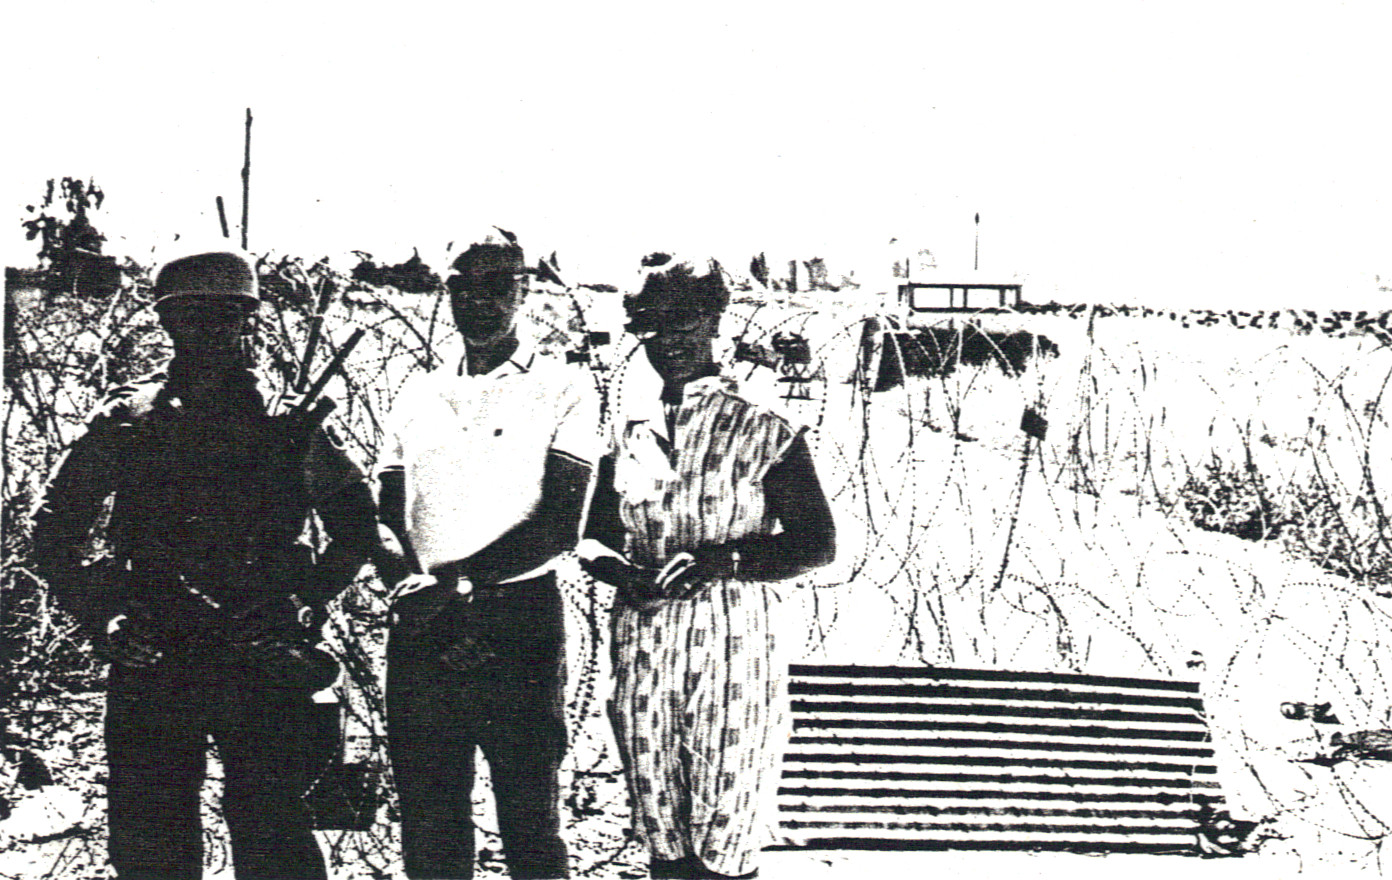
\includegraphics[width=0.9\textwidth]{photos/israel1}
  \caption{With Austrian guard at Israel-Syria border.}
  \label{israel1}
\end{figure}

All was very quiet and peaceful (apart from the strong wind which was
blowing that day) but this had been the scene of terrible battles
during the 6-day war when the Israelis were desperate to re-capture
the last area of the Golan Heights. Near here we saw the sad remains
of the Syrian Headquarters up whose steps the Israelis had driven
their huge tanks in a bid to storm and capture the Headquarters. They
succeeded.

From here there were extensive views all around but the air was quite
cold.

We proceeded to Masada, a rather different Masada from the place of
the same name on the Dead Sea and pronounced differently. This Masada
has the accent on the first ``A'' but the second ``A'' of the Masada
Fortress is accentuated.

We were to pass through lovely apple growing country and these apples
are among the nicest in the world. What a land of contrasts Israel is
-- from the point of view of cultivation alone. Obviously then, there
is a great variation of climate even in such a small country.

We came to the town of Majdal Shams which is in the centre of the
apple-growing industry and is really busy and thriving and occupied
largely, by the Druze people. The Druze are Arabs who have formed
their own sect. They are still Moslem but have differing beliefs --
for instance they believe that the next Messiah will be born of a man
and, with this in view, the men wear very baggy black trousers to make
room for the baby who might be born to the lucky one. When I said
something about the facts of life, Teddy turned the full impact of
these enormously blue eyes on me and asked if there was any more of a
``way out'' theory than the way in which our Messiah was
conceived. This was neither the time nor the place to enter into a
discussion of that nature but I could see his point of view.  Because
of the income derived from the apple industry the people here are very
rich and we saw lovely homes overlooking delightful scenery in this
high and healthy environment.  In the distance we could see Mount
Hermon (9200~ft high) whose snows help to swell the Jordan river.
This is the very high peak which is the cornerstone of Israel, Syria
and Lebanon.

We went on to Metulla and stood by the ``Good Fence'' the other side
of which is Lebanon. All was quiet and undisturbed. Teddy took a
photograph of us there (see Picture~\ref{israel2}).

\begin{figure}
  \centering
  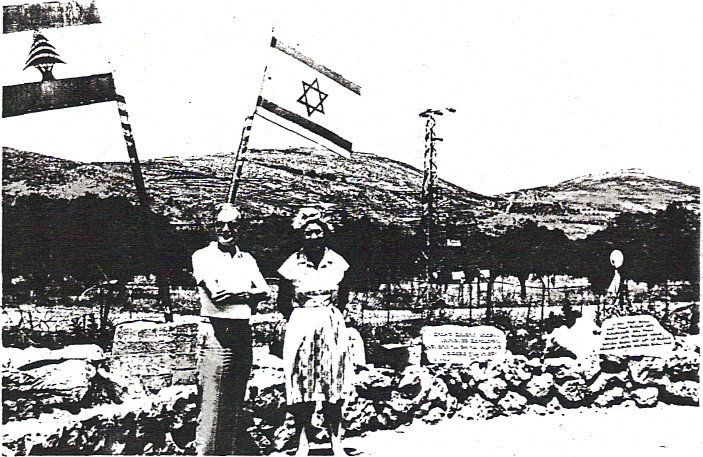
\includegraphics[width=0.9\textwidth]{photos/israel2}
  \caption{At the ``Good Fence'', bordering Lebanon.}
  \label{israel2}
\end{figure}

We were impressed by the leisurely atmosphere and old world charm of
Metullah but it must have been the centre of some very traumatic
incidents during recent wars.

On the way down from Metullah we passed Belinas, a Crusader Fort and
for quite a long time, we had lovely views of the Huleh Valley which
is extremely fertile and boasts many kibbuizim whose people look after
the crops.

We passed close by Kiryat Shmona named for the national hero, Joseph
Trumpeldor and his seven companions who, in 1920, died at the hands of
Arabs attacking the settlement of Tel Hai. The road passed very close
to the Lebanese border and we thought that Lebanon looked very
beautiful and certainly peaceful. We were now on the way to Rosh Pina
and from there to the Mount of the Beatitudes where Jesus preached the
sermon on the mount. As usual, on the site of a famous happening, a
church has been built and this again is a lovely one and in an
octagonal design; nearby is a rest house run by Franciscans. It was
amazing to hear Teddy talking to one of the Nuns in fluent Italian --
what a versatile man he is! Once more we saw beautiful and ancient
mosaics, this time mainly concentrated on the ceiling of the
church. Teddy persuaded one of the many tourists to take a photograph
of the three of us (see Picture~\ref{israel3}).

\begin{figure}
  \centering
  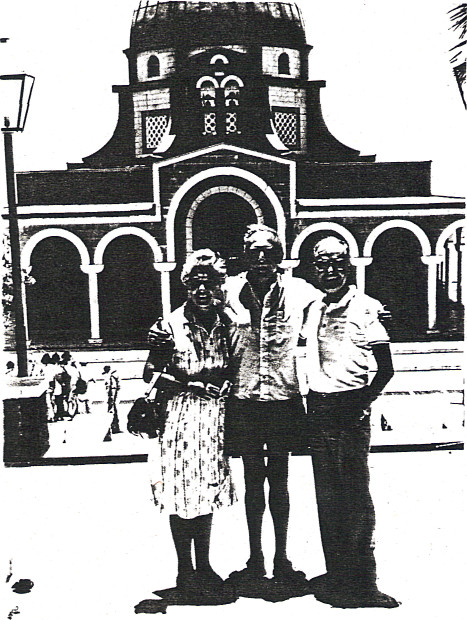
\includegraphics[width=0.9\textwidth]{photos/israel3}
  \caption{Madge, Teddy Vardi, and Tony at the church on the Mount of
    the Beatitudes.}
  \label{israel3}
\end{figure}

Soon we were on our way back to Tiberias - I think it was because we
had seen so much of interest that we seemed to have travelled further
than we did; in fact, we covered about 200~km that day and were to
travel approximately the same distance on the following day. We
stopped at a place called Banias which is one of the sources of the
River Jordan. Hillocks, rivulets and a lovely park create a beautiful
setting for the pagan temple of the God Pan whose image is carved in a
cave on the hill. We put our hands into the cool clear water.


\section{June 14th}

We got back to Tiberias tired but happy and on Thursday June 14th we
had to leave it -- Tiberias with its exquisite scenery, delicious
St. Peter's fish and unforgettable scenes of New Testament
reference. We promised to return some day!

We went on the road to Rosh Pina, the first of the Jewish settlements
in Galilee and, from there, to Safed. Teddy pronounced it Zfat and,
according to various signposts, it did seem to have several different
pronunciations to choose from.

Safed was entirely destroyed by an earthquake in 1836 but has been
charmingly rebuilt with colleges and art galleries etc.

The view from the car as we climbed up to Safed was breathtaking and
we felt the temperature falling which was welcome as the day was
already hot. The air was cool and invigorating and it is not
surprising that people visit this place to convalesce as there is a
Health giving spa as well as the superb climate. The wind sighing
through the pine trees was the sound of music.

Safed was once a fortress, not surprising in view of its high key
position, but now it is the home of students of the Cabbala a
mediaeval philosophy of direct communication between Man and God. We
visited two synagogues, one to the memory of Joseph Caro, a remowned
Rabbi and Scholar. Both the synagogues were small but quite exquisite.

Tony and I wandered through an Art Gallery but we were not inspired by
the Israeli style of Art either here or in any of the other galleries
we visited. Chagall is a different ``kettle of fish'' altogether.

It seemed a shame to have to leave the cool and invigorating
atmosphere of Safed and descend to the heat of the valley but we now
looked forward to our first visit to a Kibbutz -- Kibbutz Sasa --
which Teddy had helped to start and where he had lived for 8 years.

The kibbutz system is Communism with a small ``c'' and outside of
Israel, people seem to be very sceptical about it but it really does
seem to work with all the members, sometimes whole familes, of the
right mind to accept and contribute to the communal way of life. There
are strict rules of life and everything is well organised; if one
member shows any intellectual or any other kind of promise, funds are
used from the Kibbutz to further his education and some famous
Israelis started life in a kibbutz.

Teddy was thrilled to find that a new concert hall complete with
proper theatre type seats had been built since he was there. He was,
obviously, very proud of the place and it did look pretty and well
cared for. We got into chance conversation with a girl from Andover in
Hants -- once more a very small world!

Teddy promised to arrange for us to stay in a kibbutz next time; some
of them have well run guest houses which, of course, contribute to the
much needed income.

We proceeded on our way and saw signs to such places as Maalot, and
Nahariya but we were actually making for Acre which is Akko in the
Bible.

This interesting place attracted the first Canaanite settlers 4,000
years ago. It was fascinating to realise that there were several Acres
below the one upon which we walked and the history of it would take a
very long time to absorb -- it having passed through the rules of
Canaanites, Jews, Greeks, Romans, Crusaders, French, Turks etc., but
it would appear to the tourist that the Crusaders have left the
strongest mark although there is a very beautiful Turkish Mosque which
we did not have time to visit. It was with some awe that we were taken
to the subterranean Crypt of St. John and the Hospitaller, both of
which are absolutely huge and somehow, full of the atmosphere of
bygone days. We walked out on to the sea walk which of course provided
a grand view of the ancient Harbour (see Picture~\ref{israel4}).

\begin{figure}
  \centering
  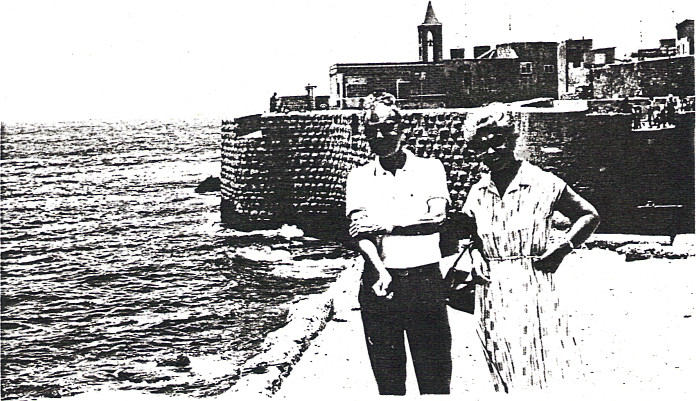
\includegraphics[width=0.9\textwidth]{photos/israel4}
  \caption{Tony and Madge beside the harbour at Acre.}
  \label{israel4}
\end{figure}

We would have enjoyed a much longer sojourn in Acre but time was
pressing. I felt that the volume of history was just crying out to be
absorbed but, unfortunately, we had to be on the move -- perhaps there
will be another occasion to visit Acre.

In the car again and on our way to Megiddo, we could see the Port of
Haifa on the opposite Point of the Bay as we passed below
Mt. Carmel. Megiddo is destined to be the site of the Final battle
between Good and Evil and Armageddon is the name given to this battle.

There has been expert and unbelievable excavation carried out by the
Oriental Institute of the University of Chicago and, at one place, it
is possible to look down a "Cut" and see 16 layers of civilization;
this was just too much to take in!

The energy and patience of archeologists are to be greatly admired and
it is not difficult to imagine the thrill and sense of achievement
asdf when some important discovery is made.

We found it paid dividends to examine the beautiful model of Megiddo,
ancient walled city of the 15th Century, BCE, before walking round the
site. This made the discovery of the partially restored walls, the
stepped water shaft leading to the water source, (unfortunately closed
on that day) the stables, palaces and storehouses much easier to
comprehend. It would have taken hours to explore the site for it is
huge. The heat was terrific in spite of the strong breeze. All around
us were extensive and lovely views and, Megiddo once having been a
hi11-Top Fortress, it was easy to see that it commanded a key position
and clear view of approaching enemies. On to Caesarea which boasts the
only Golf course in Israel! Caesarea was named for Augustus Caesar and
was under Roman rule for 600 years. From here St.~Paul set out for
some of his missions abroad. Once more, the Crusaders left a very
strong mark.

Teddy took us to a place where there are the remains of statues --
mostly headless and armless -- remains of the Roman era. They had been
beautifully carved, the folds of the garments looking very real. Teddy
took a photograph of us there and it is to be hoped that our friends
will be able to distinguish us from the statues (see
Picture~\ref{israel5})!

\begin{figure}
  \centering
  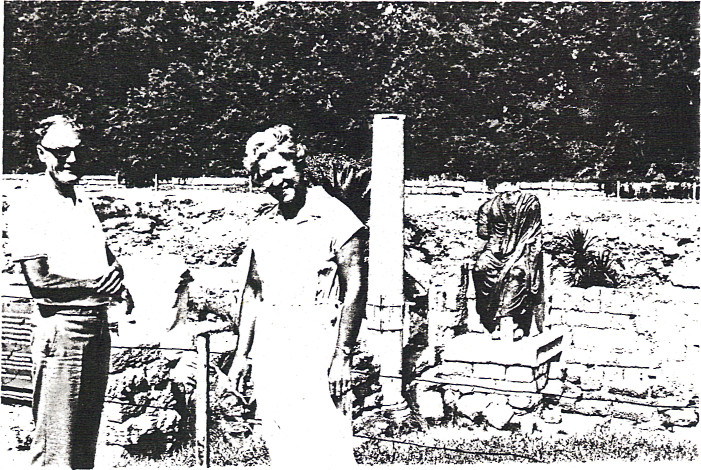
\includegraphics[width=0.9\textwidth]{photos/israel5}
  \caption{Tony and Madge beside statues at Caesarea.}
  \label{israel5}
\end{figure}

On to Natanya, the centre of Israel's diamond industry and the home of
the largest diamond exchange in the world. In this building we were
invited to watch a film about diamonds, which was very interesting,
and to observe some craftsmen filing those 58 facets on the precious
stones. Like a lot of very difficult crafts, it looked remarkably easy
and quick but it must take years of practice to develop such a skill.

It was interesting, and somewhat comforting -- to learn that it is
impossible for diamonds to lose their value; they can only appreciate
with time. We were taken to a lovely showroom where magnificent pieces
of finished jewellery were on display. One was now encouraged to buy
and some tourists were doing so but we were not certain of our dollars
even though we were coming to the end of our holiday. We had several
accounts still to settle and it would have been unwise to overspend at
this stage -- even so there were some ``mouth watering'' pieces to be
seen.

So firmly into the car and back ``home'' to Tel Aviv where we again
booked into the lovely ``Sheraton''. After some refreshments, we
regretfully had to say ``Goodbye'' to Teddy who had become a real
friend and companion during our travels together as well as being a
fantastic source of information. We felt sad at seeing him off but I
am sure this was not the end of our association. I do wonder what he
would think of what I have written...

I must admit to feeling a little lost back in Tel Aviv for we had
suddenly come to the end of culture and history and had absorbed a
surfeit of it but it was nice, after all, to look at the beautiful
Mediterranean from our balcony and to listen to the ever attractive
sounds of the sea. We had had a full day and had spent a lot of it in
the full blast of the sun which always induces tiredness, so after
baths and a customary stroll along the beach, we had a light supper
and went to bed quite early.


\section{June 15th}

Tony had business to do with the Telrad people on Friday morning, so I
used the time to catch up on my notes. I was going to wander to the
beach but it was suddenly lunchtime and Tony appeared to take me
downstairs to have something to eat.

We watched a video in the afternoon and then after the usual little
walk it was time to get ready for our Shabbat dinner invitation from
Gurion and Sara Meltzer.

As I have already written, this Friday night dinner is the highlight
of the week for Jewish families and it was therefore a great honour
for us, as Gentiles, to be invited.

Gurion and Sara are strict Orthodox Jews. Beno and Felya Ellman were
also invited and since they were coming to Johannesburg for a term of
duty shortly afterwards, it was pleasant to meet them beforehand, and
I suspect encouraging for them to know that there would be a least 2
familiar faces for them to see in an unfamiliar place. We liked them a
lot and, of course, Gurion and Sara are two of the most wonderful and
genuine people it is possible to meet.

We enjoyed Sara's delicious food and, throughout the meal, we were
fascinated by the rituals attached to it. Gurion explained each step
and ritual as we went along and the reasons why he blessed and
distributed the wine in a certain way and why a piece of bread was
cut for each member of the family whether they were present or
not. Prayers were said throughout the meal and with typical
thoughtfulness, Gurion provided us with prayer books in English so
that we would be able to follow the prayers which he was reciting oh!
so quickly.

This occasion was a memorable one for us; there was no restraint in
the conversation and the atmosphere was most friendly and
relaxed. Sara's mother, daughter and small grandson were present and
so it was a family occasion as well as being one to delight visitors.

The evening came to an end and we took our leave of them all with
thanks for allowing us to join them.


\section{June 16th}

Saturday was our last day in Israel and we had to decide what to do
with it but that did not take long. We would return to Jerusalem, a
distance of 50 km, and take a last fond look at the Old City. By this
time, it was evident that there would be dollars to spare for some
mementos of our visit so I decided that I would like to have the oil
lamp and filler I had seen in the Baidoun shop -- little did I know
that we would come away with a wine carafe as well.

The hotel doorman found us a very pleasant taxi driver who chatted to
us all the way to Jerusalem and promised to be waiting for us outside
the King David Hotel at a certain time -- and he was there on the dot.

Once more, Tony and I found great pleasure in walking though the Old
City, parts of which were by now, quite familiar to us. We found our
way to Mr Baidoun very easily and spent a pleasant hour chatting to
him and an American archeologist who assured us that anything we
bought in this shop was authentic -- indeed we were given certificates
of authenticity for our three purchases. How glad I am that we decided
to buy something worthwhile and valuable, there was so much ``junk''
there and I could not believe my eyes when I saw some Americans buying
``Crowns of Thorns''. Heaven knows how much they paid for them.

This had to be our final ``Farewell'' to the Old City and to
Jerusalem. I had so enjoyed my visits there and can still remember it
all vividly. Of the great number of impressions to be gained, I
believe that my chief one is amazement at the religious tolerance
which abounds. This, after all, is the home of the three great faiths,
all apparently living comfortably side by side... and Ireland cannot
cope with 2 offshoots of the same one!

The last evening in Tel Aviv was spent in the company of Gurion, Sara,
Ami and Osnat, for we had invited them to have dinner with us at our
hotel in the ``Twelve Tribes'' restaurant.

This was a lovely and enjoyable climax to our holiday and, of course,
they were all eager to learn of our impressions of their fabulous
country; naturally we were able to assure them that we were delighted
with everything we had seen and that we hoped, one. day, to return and
see those parts of Israel we had not had time to explore.

A lovely evening with good company, and good food in pleasant
surroundings is hard to beat.

Eventually we took our leave of them with promises to meet again
either in Israel or South Africa.

A lovely flight the next day by El Al to London and the start of
another glorious holiday but with so many memories of a happy time.

May we return one day.

    %\chapter{Pictures}

% \begin{figure}
%   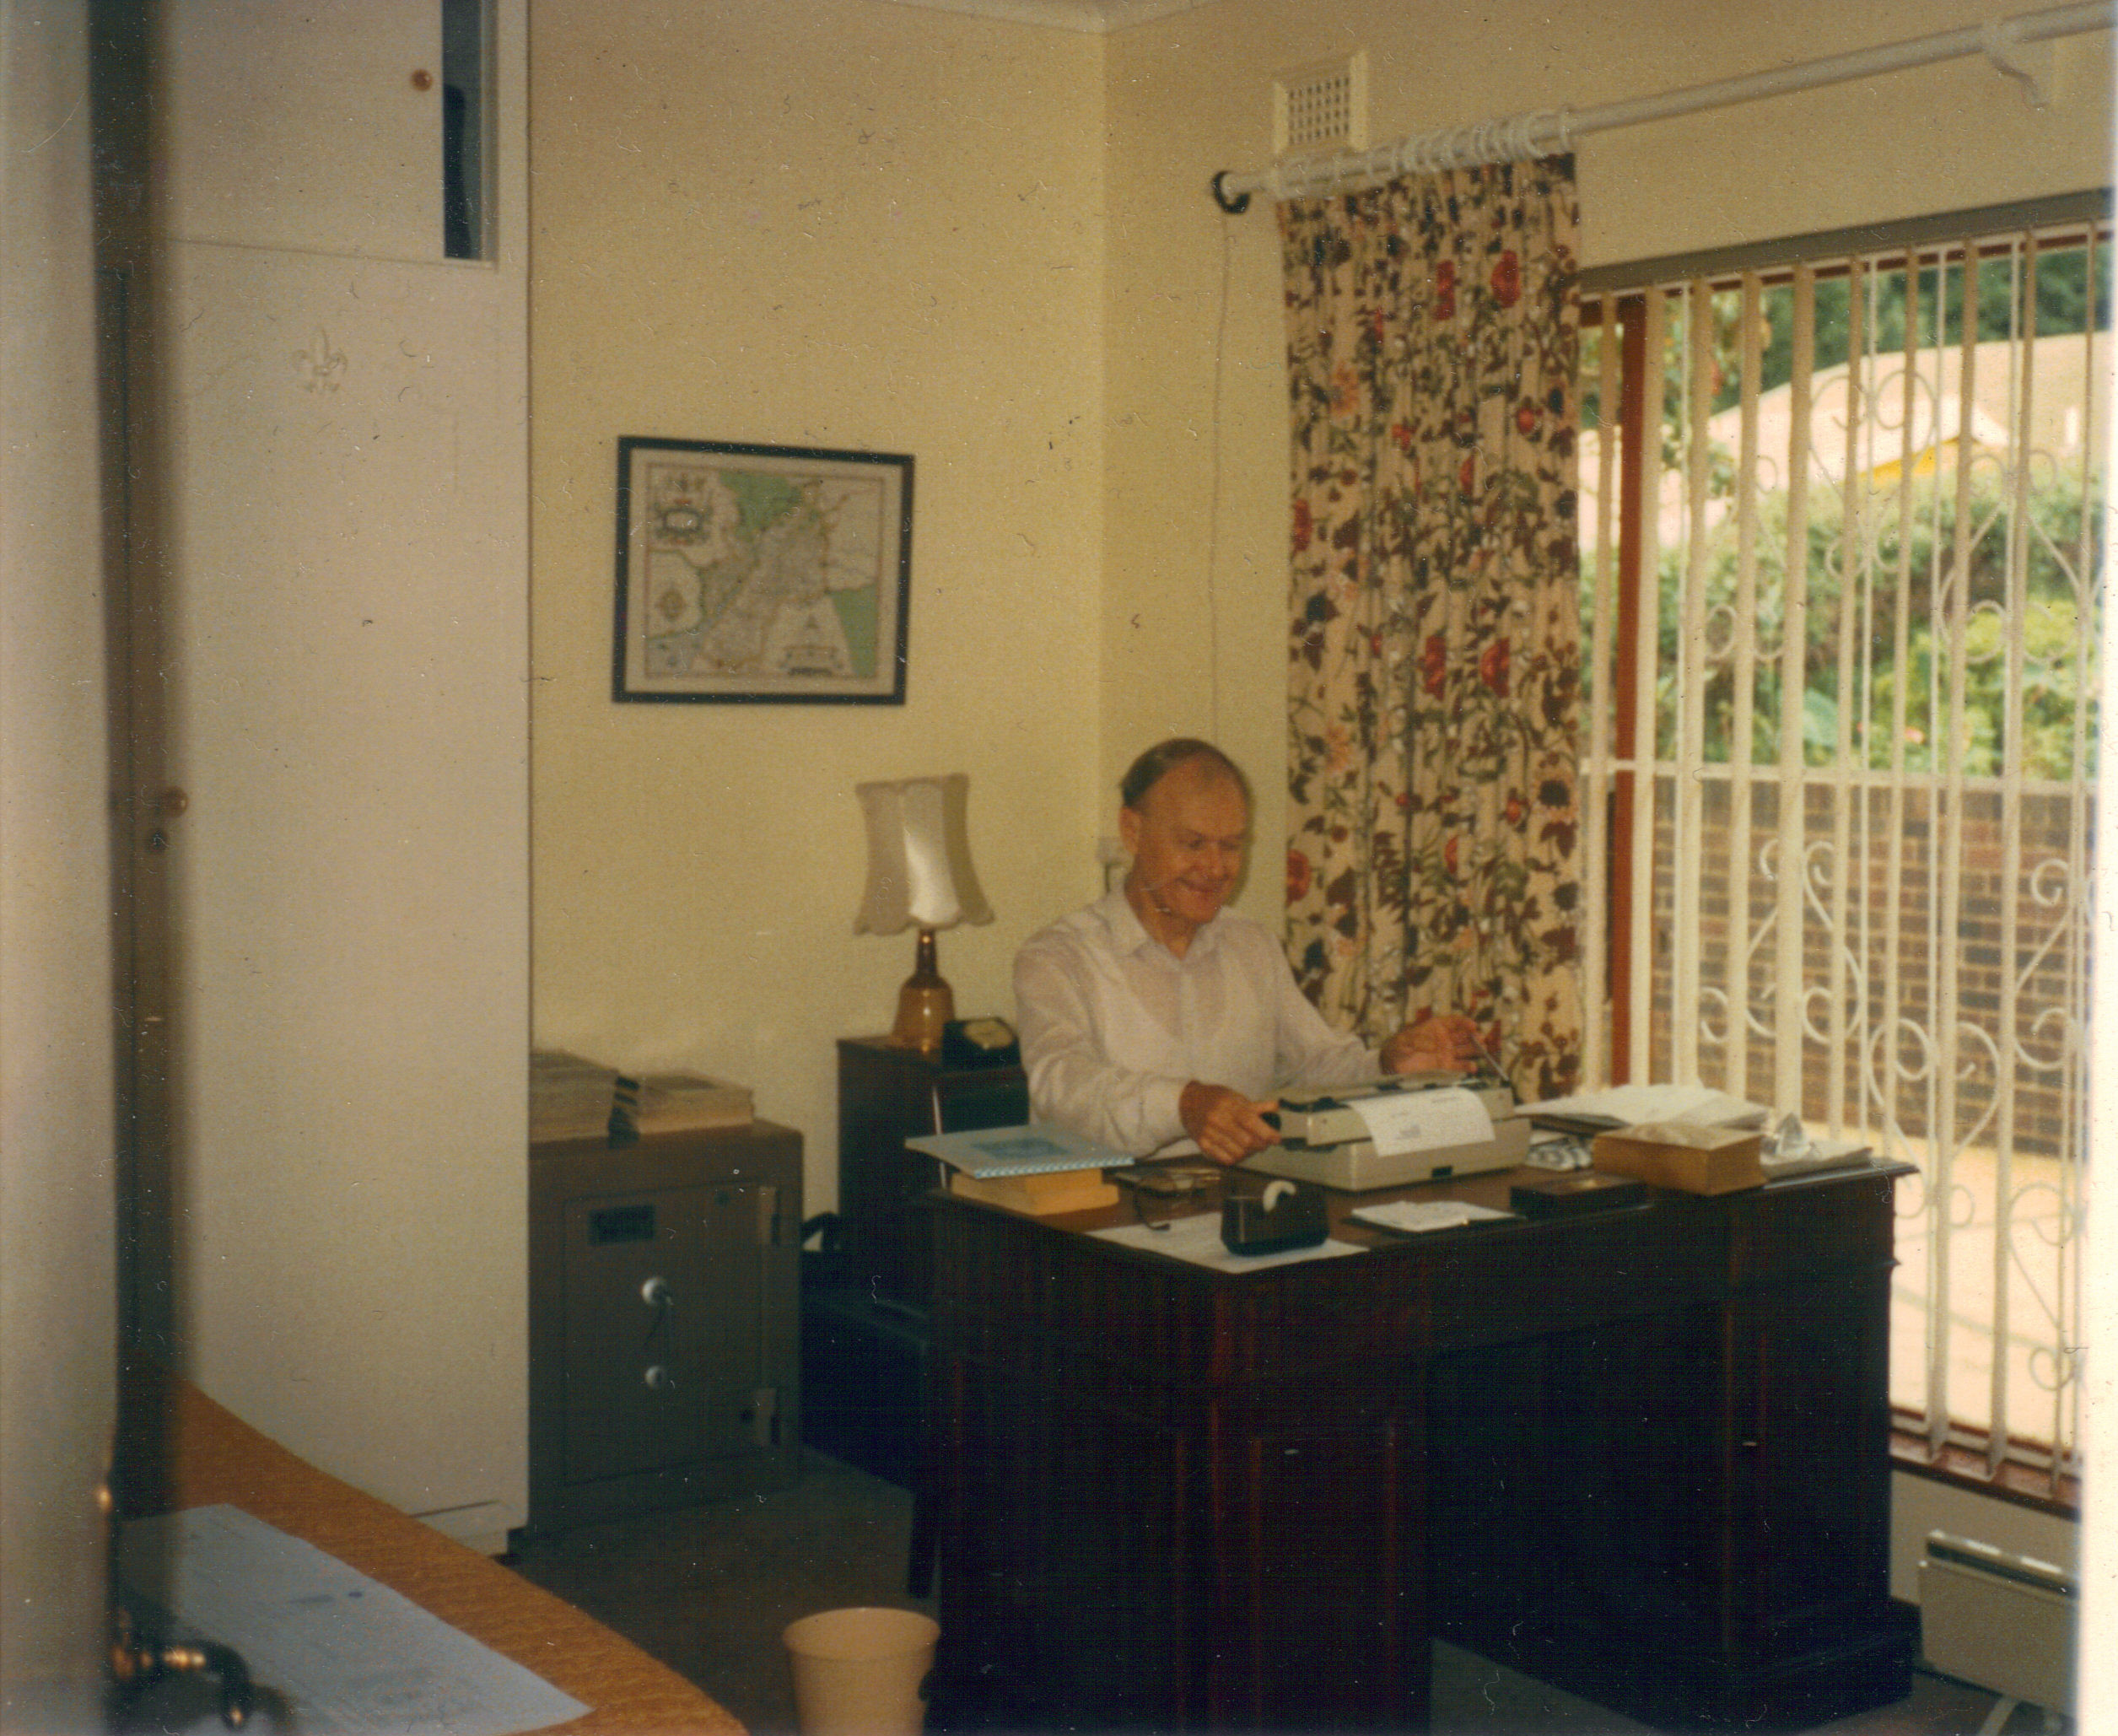
\includegraphics[width=\textwidth]{photos/tony-office}
%   \caption{Tony in his Hillcrest office.}
%   \label{tony-office}
% \end{figure}

% \begin{figure}
%   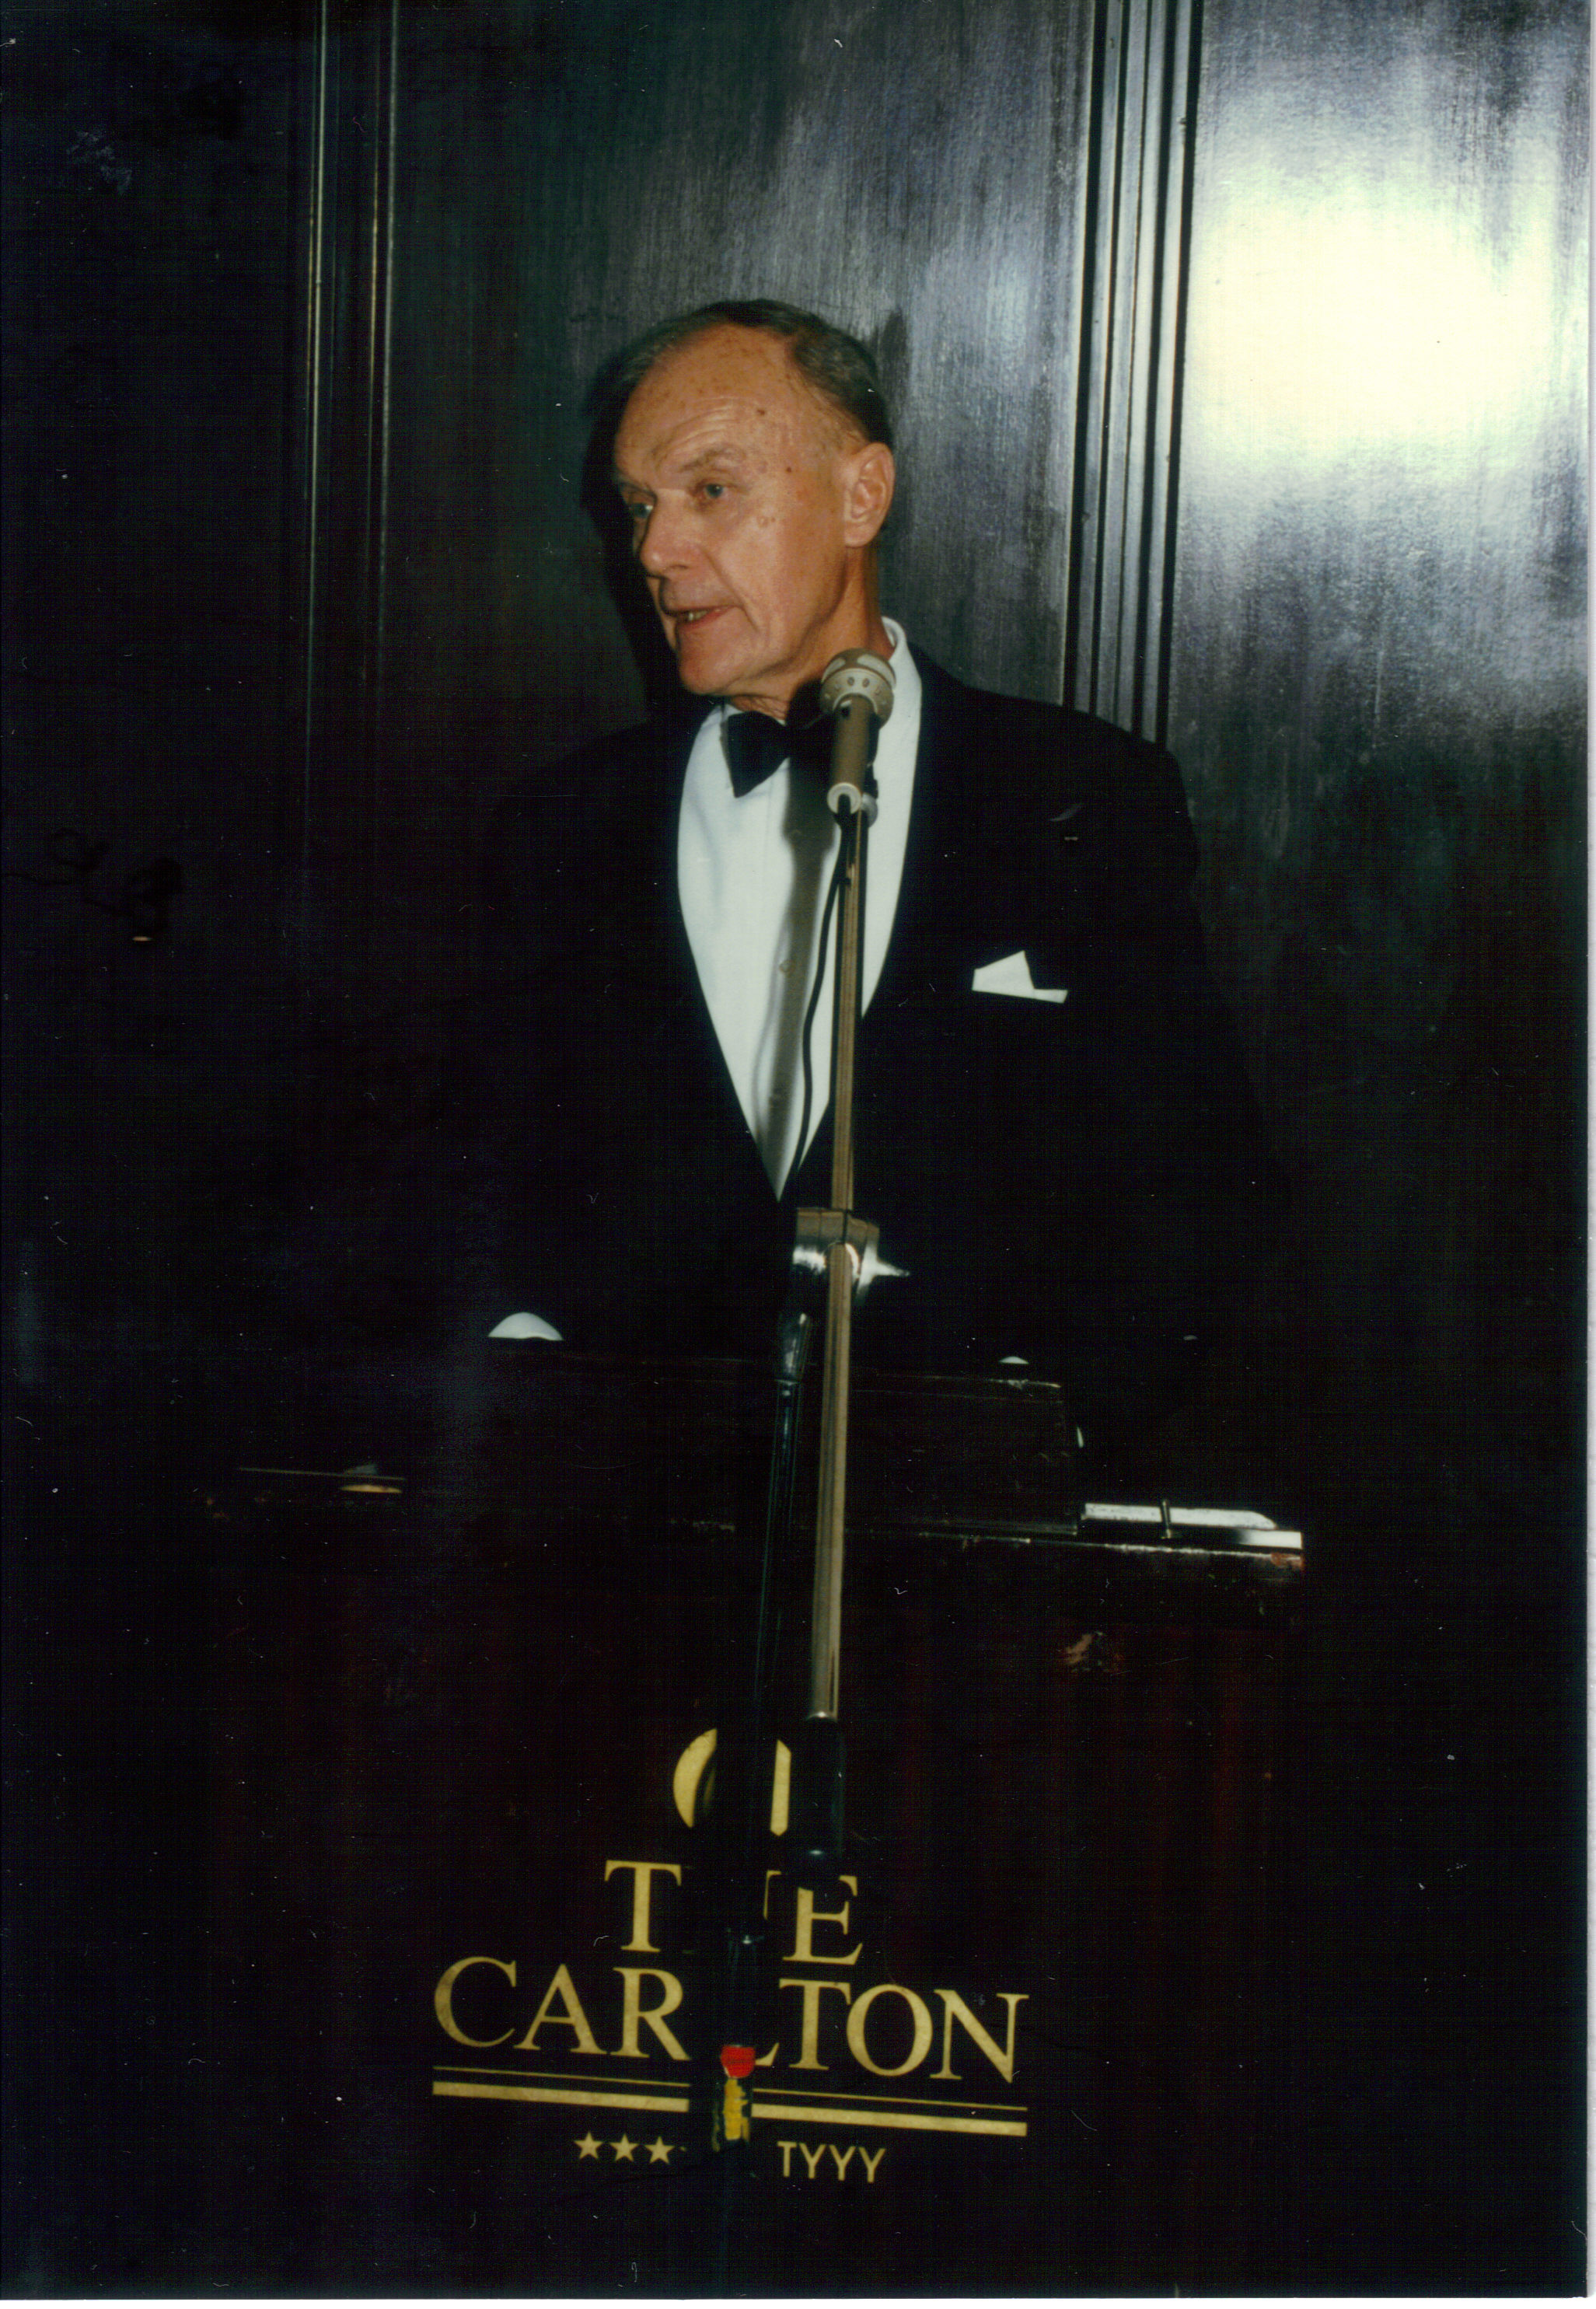
\includegraphics[width=\textwidth]{photos/tony-speaking}
%   \caption{Tony speaking at ???.}
%   \label{tony-speaking}
% \end{figure}

% \begin{figure}
%   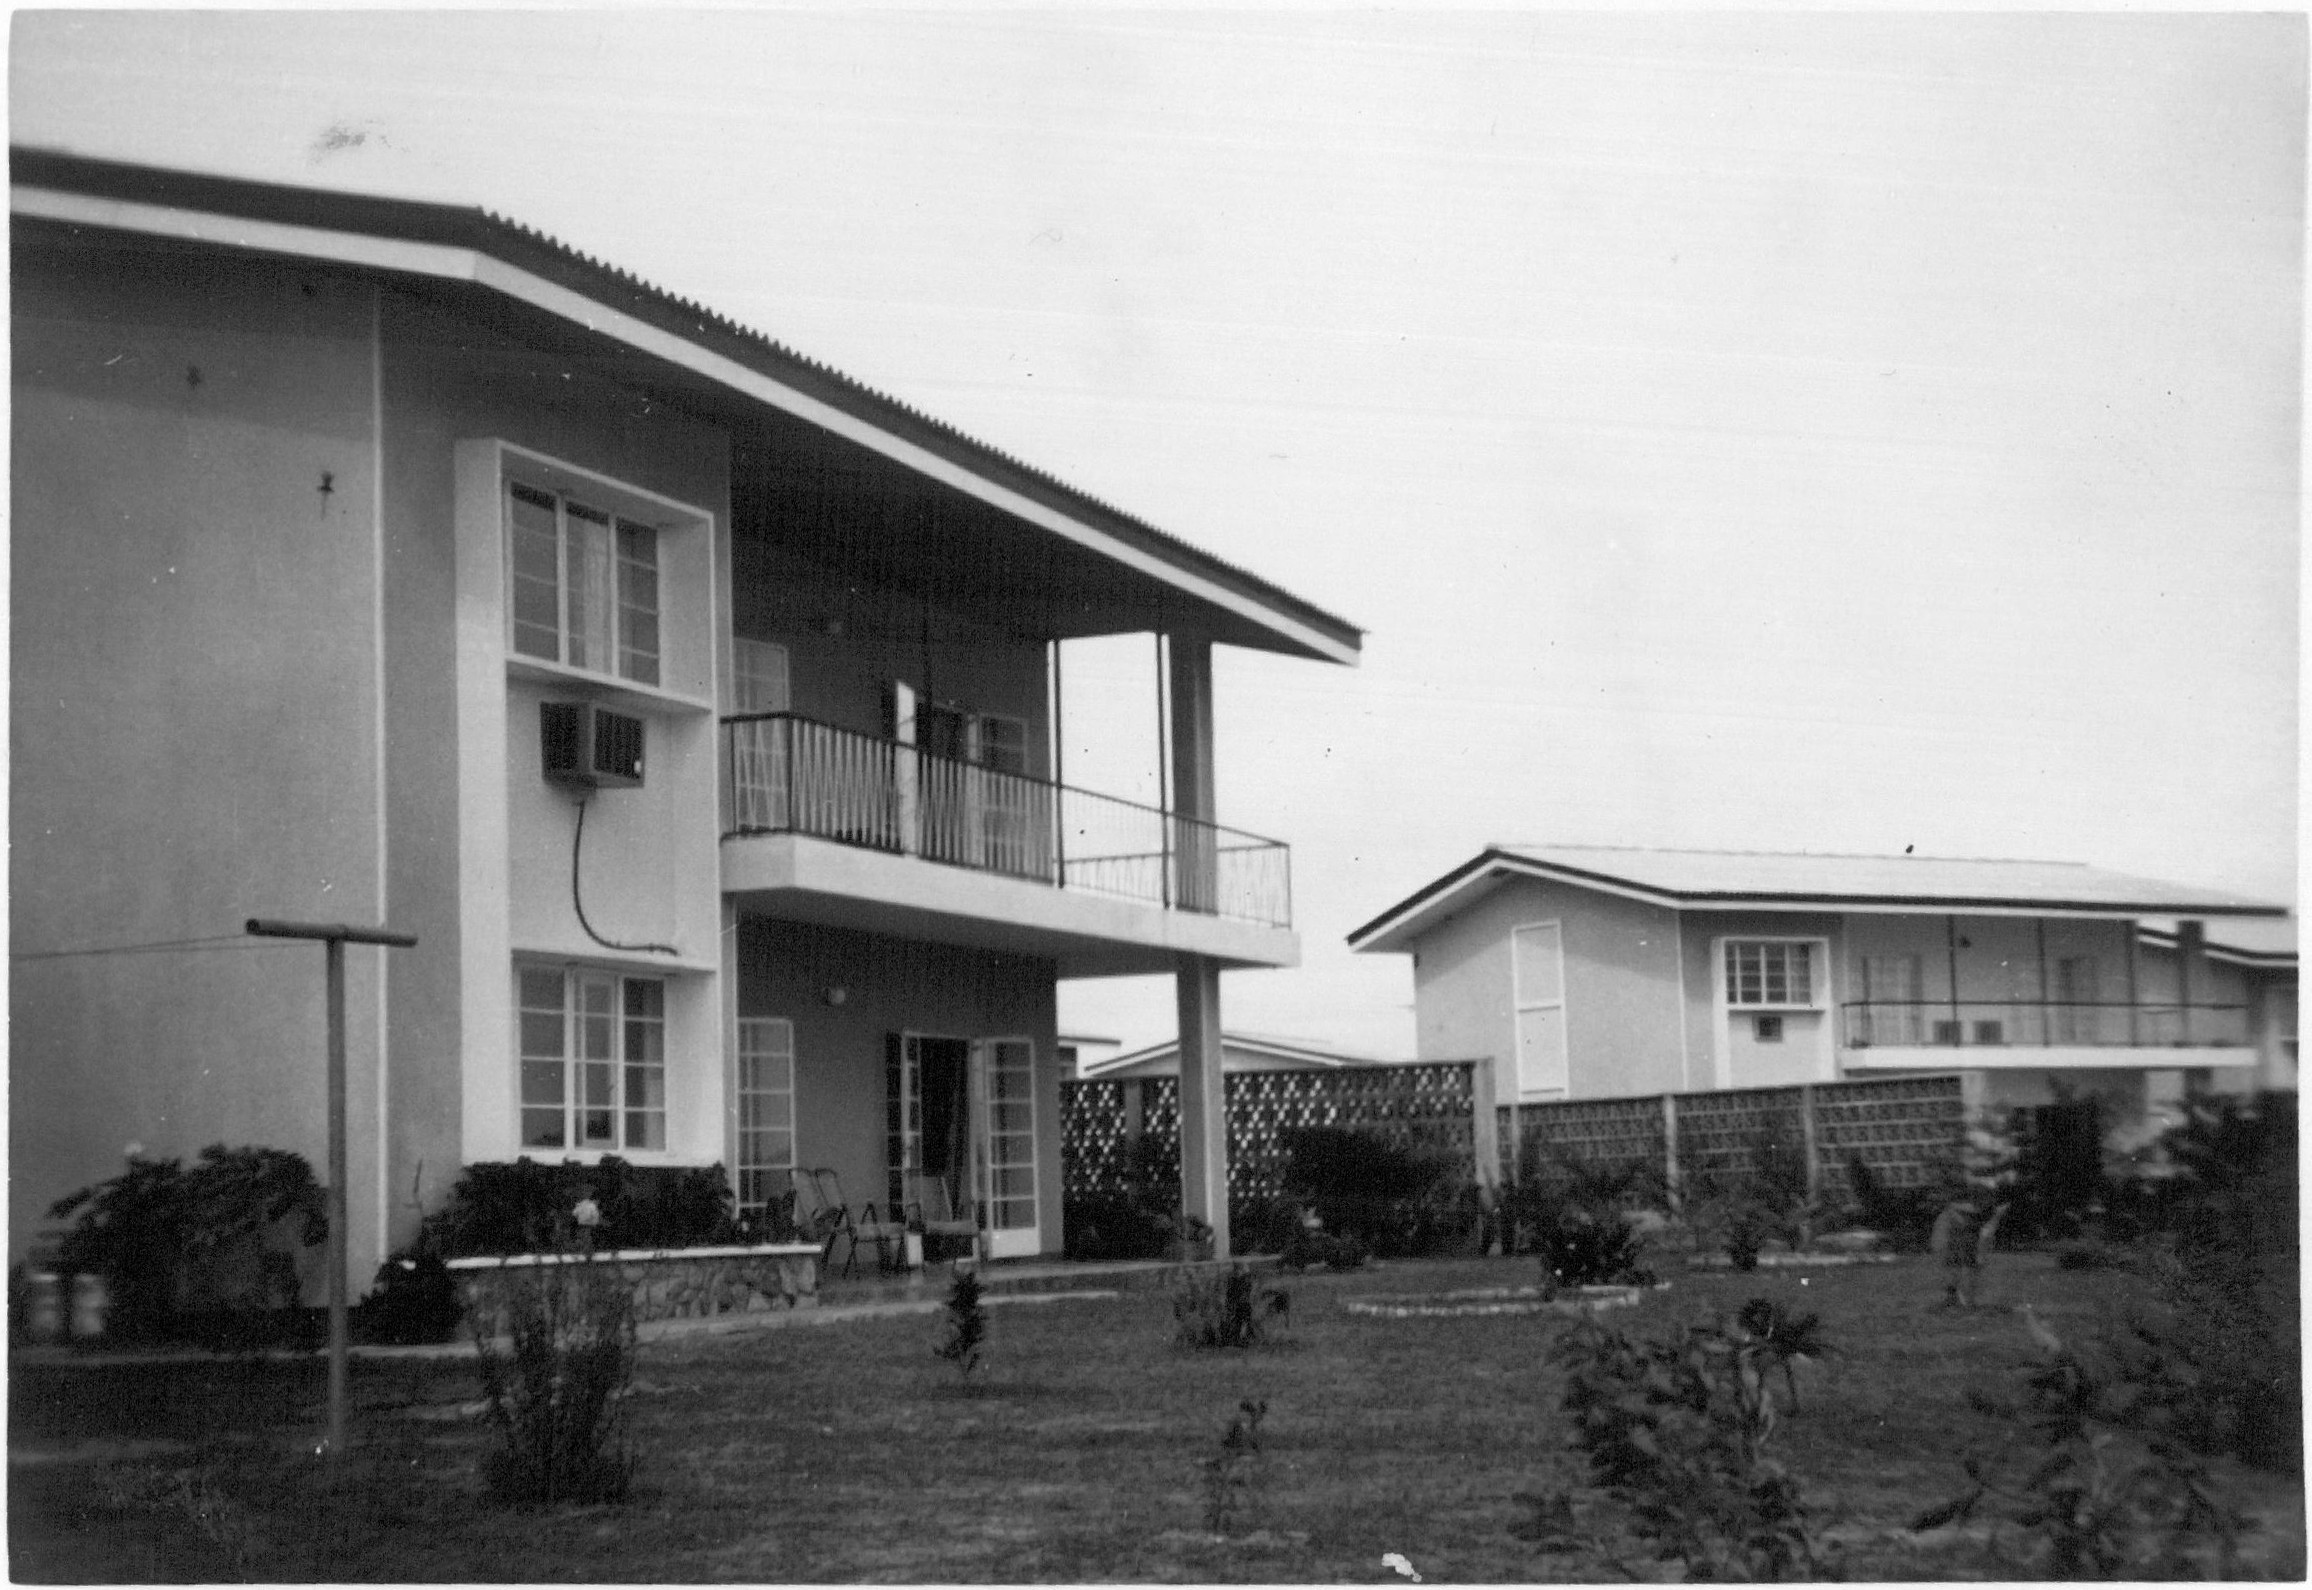
\includegraphics[width=\textwidth]{photos/house}
%   \caption{The Bray family house in Lagos.}
%   \label{house}
% \end{figure}


\backmatter

\end{document}
